%Thomas North University of Birmingham Thesis
%A thesis normally consists of the following elements:
%• Author’s Declaration Form (Library deposit copy only)
%• Preliminaries
%- title page
%- abstract
%- dedication
%- acknowledgements
%- contents listings
%- table of contents
%- list of illustrations
%- list of tables
%- list of definitions and/or
% abbreviations
%• Text
%• End Pages
%- appendices
%- list of references/bibliography

%%%%%%%%%PACKAGES%%%%%%%%%%%%%%
\documentclass[a4paper, 12pt, oneside]{report}
\usepackage[doublespacing]{setspace}

\usepackage[top=3cm, bottom=3cm,inner=3cm,outer=3cm]{geometry}
\usepackage{aas_macros}
\usepackage{amsmath,amssymb,graphicx,natbib}
\usepackage{enumerate,relsize,float}
\usepackage[compact]{titlesec}
\usepackage{comment}
\usepackage{threeparttable}
\usepackage[hidelinks]{hyperref}	% Hyperlinks
%\hypersetup{colorlinks=True,linkcolor=blue,citecolor=blue,filecolor=blue,urlcolor=blue}
\usepackage{xspace}
\usepackage{longtable}
\usepackage{bm}
\usepackage{subfig}


%%%%%%%%%%%%%%%%%%%%%%%%%%%%%%%%%%%%%%%%%5
\graphicspath{{Title/}{Chapters/Intro/}{Chapters/HiSPARC/}{Chapters/HS_14008/}}%Add more folders here for graphics for each chapter. 

%%%%%%%%%%%%%%COMMANDS%%%%%%%%%%%%
\newcommand{\Ms}{\ensuremath{\textrm{M}_{\odot}}\xspace}
\newcommand{\Me}{\ensuremath{\textrm{M}_{\oplus}}\xspace}
\newcommand{\Mj}{\ensuremath{\textrm{M}_{\textrm{J}}}\xspace}
\newcommand{\Rs}{\ensuremath{\textrm{R}_{\odot}}\xspace}
\renewcommand{\Re}{\ensuremath{\textrm{R}_{\oplus}}\xspace}
\newcommand{\Rj}{\ensuremath{\textrm{R}_{\textrm{J}}}\xspace}
\newcommand{\Ls}{\ensuremath{\textrm{L}_{\odot}}\xspace}
\newcommand{\e}[1]{\ensuremath{\times 10^{#1}}}
\newcommand{\numax}{\ensuremath{\nu_{\textrm{max}}}\xspace}
\newcommand{\delnu}{\ensuremath{\Delta\nu}\xspace}
\newcommand{\teff}{\ensuremath{T_{\textrm{eff}}}\xspace}
\newcommand{\logg}{\ensuremath{\log{g}}\xspace}
\newcommand{\feh}{\ensuremath{\textrm{[Fe/H]}}\xspace}
\newcommand{\mdash}{\xspace{---}\xspace}
\newcommand{\ndash}{\xspace{--}\xspace}
\newcommand{\Kepler}{\ensuremath{\emph{Kepler}}\xspace}
\newcommand{\tabgap}{\noalign{\vskip 1mm}}

\setcounter{secnumdepth}{3}
%\renewcommand{\thechapter}{\Roman{chapter}}
%%%%%%%%%%%%%TWEAKS%%%%%%%%%%%%%%%%%
% Tweak chapter headings
%\titleformat{\chapter}[display]{\Huge\center}{\chaptername\,\,\thechapter}{0pt}{}{}
\titleformat{\chapter}[hang]{\Huge\center}{\thechapter}{1em}{}{}
\titleformat*{\section}{\Large\bfseries}
\usepackage[font=small]{caption}
\setcounter{tocdepth}{1}


\begin{document}
\doublespacing
\pagenumbering{Roman} 

%TITLE PAGE
%Thesis Title Page
\begin{titlepage}
\vspace{6cm}
\begin{center}
\begin{doublespace}
{\Huge \bf Thesis Title}
\end{doublespace}
\vspace{1cm}
by\\
\vspace{1cm}
{\Large E. Ross}\\
\vspace{2.5cm}

\includegraphics[scale=0.35]{onlyunilogo.png}\\
\vspace{2.5cm}
A thesis submitted to the \\
University of Birmingham \\
for the degree of \\
DOCTOR OF PHILOSOPHY\\
\end{center}
\vfill
\begin{flushright}     
Solar and Stellar Physics Group (SASP)\\
School of Physics and Astronomy \\
University of Birmingham \\
Birmingham, B15 2TT\\
Month 20XX\\
\vfill
\end{flushright}
\end{titlepage}

%  Abstract 
\chapter*{Abstract}

The solar cycle gives rise to complex structures and dynamics in the outer layers of the Sun. As a result of magnetic disturbances on the Sun, large bursts of energy lead to space weather effects that can be potentially harmful to life on Earth. In this thesis, we present a series of projects exploring the themes of \gls{cr} space weather applications and understanding the solar interior-atmosphere linkage. 
%Solar activity varies periodically, which is known as t

A feasibility study was performed to determine whether the \gls{hisparc} network was suitable for detecting space weather events. Using simulations and \gls{hisparc} data, evidence suggested this was unfeasible. We introduced a new configuration of \gls{hisparc} station, which minimised \gls{cr} energy biases and noise. This configuration was demonstrated to improve the capabilities of \gls{hisparc} a space weather monitor.
%properties and data of five \gls{hisparc} stations were examined in detail, and we showed there were no clear observations of \glspl{gle} or \glspl{fd} in the data. \gls{as} simulations were performed to further explore the response of \gls{hisparc} and our predictions suggested that variations from \glspl{gle} would be minimal.
%demonstrated the performance of this station, including the mean count rate, noise, and response to \glspl{gle}, to demonstrate its capabilities as an improved space weather monitor.

Long-term variations of \glspl{gcr} versus \gls{ssn} during recent solar cycles explored the relationship between solar activity and \glspl{gcr}. Focussing on the most recent cycle---24---we showed it behaved in-accordance with previous even-numbered cycles.
%A study of the l


Finally, a frequency-domain analysis of over 20~years of high-cadence \gls{bison} observations of the \gls{smmf} was presented. This provided evidence to suggest the strongest component of the \gls{smmf} is connected to \glspl{ar}, based both on the inferred lifetime and location on the solar disc.
%Acknowledgements
\chapter*{Acknowledgements}
\thispagestyle{plain}

Firstly I would like to sincerely thank my supervisor, Professor Bill Chaplin. Thank you for inspiring me to enjoy solar and stellar physics as a undergraduate, for your advice and support throughout this Ph.D., and also for allowing me the freedom to explore other creative ventures during my studies.

I would also like to thank my secondary supervisor, Professor Cristina Lazzeroni, for expert support during my Ph.D. and offering me opportunities to get involved in outreach and engagement activities during my studies.

I would also like to thank Dr. Angela Romano and Dr. Francesco Gonnella for their incredible support. In addition, thank you to Dr. Steve Hale for advice and for allowing me on a trip to Carnarvon. My experience was made much easier with their guidance.

A special thank you to all colleagues within and connected to the Solar and Stellar Physics (SASP) group, or Sun, Stars, and Exoplanets (SSE) group, and in the Astrophysics and Space Research (ASR) group. I would particularly like to thank my incredible fellow Ph.D. students: Vedad, Tom, Ben, Mat, Oli, Alex D., Saniya, Matt, Walter, George, Emma, Alex L., Lindsey, and Emily, for some fantastic memories. The games, drinks, meals out, tea breaks, and friendship all made my experience absolutely delightful. Furthermore, thank you to the postdocs: Ted, Martin, Warrick, Matteo, Jake, and Elinore.

This Ph.D. would not have been possible without the work of the staff in the School of Physics and Astronomy and the wider support staff at the University of Birmingham. Thank you namely to Kat Grover, Lou Barden, Maria Pavlidou, and Holly Prescott; in addition to the staff in the Physics and Astronomy stores and the education support office.

Thank you to my family for supporting me through the Ph.D.: Mum, Dad, Hayley, Chris, and Connor. Thank you to all my friends, new and old, who have been a part of this with me. Finally, an enormous thank you to Dr. Hannah Serrage whose enthusiasm, kindness, and wisdom has helped me tremendously through this odyssey.

Finally, thank you to my reviewers and editors, and my thesis committee.
%  C O N T E N T S ,   T A B L E S  ,   F I G U R E S ,   N O T A T I O N
\newpage
\pagestyle{plain}
\begin{singlespace} %Optional singlespacing
\tableofcontents
\thispagestyle{plain}
\addtocontents{toc}{\protect\thispagestyle{plain}}
% Uncomment the following four lines to include a list of figures
\listoffigures
\thispagestyle{plain}
\addtocontents{lof}{\protect\thispagestyle{plain}}
\thispagestyle{plain}
%add tables too
\listoftables
\thispagestyle{plain}
\addtocontents{lot}{\protect\thispagestyle{plain}}
\thispagestyle{plain}

%  Abbreviations
\thispagestyle{plain}
%\addcontentsline{toc}{chapter}{List of Abbreviations}
\chapter*{Abbreviations}
\thispagestyle{plain}

\begin{tabular}{l l}
	{ADC} & {Analogue to Digital Converter} \\
	{AS}		&	{Air Shower}	\\	
	{AVD}  & {Asymptotic Viewing Direction} \\
%	{BDS}	&	{Bi-Directional Streaming}	\\	
	{BiSON}  & {Birmingham Solar Oscillations Network} \\
%	{CG}		&	{Compton Getting}	\\	
%	{CIR	}	&	{Corotating Interaction Region}	\\	
	{CMA} & {Central Moving Average} \\
	{CME}	&	{Coronal Mass Ejection}	\\
	{CR}	&	{Cosmic Ray}	\\		
	{EAS}  &  {Extensive Air Shower} \\
	{EV}		&	{Enhanced Variance}	\\
	{FD}		&	{Forbush Decrease}	\\
	{FE}		&	{Forbush Effect}	\\
	{FOV}	&	{Field Of View}	\\
	{GCR}	&	{Galactic Cosmic Ray}	\\
	{GIC}   &  {Ground Induced Current} \\ 
	{GLE}	&	{Ground Level Enhancement}	\\
	{GMDN}	&	{Global Muon Detector Network}	\\
	{GNSS} & {Global Navigation Satellite System} \\
	{GZK}  &  {Greisen-Zatsepin-Kuzmin} \\
	{HCS}	&	{Heliospheric Current Sheet}	\\
	{HiSPARC} & {High School Project on Astrophysics and Research with Cosmics} \\
	{ICME}	&	{Interplanetary Coronal Mass Ejection}	\\
	{IMF	}	&	{Interplanetary Magnetic Field}	\\
	{LC}		&	{Loss Cone}	\\		
	{MD}  & {Muon Detector} \\
	{MFP}	&	{Mean Free Path}	\\																
	{MIP} & {Minimum Ionising Particle} \\
	{MOSWOC}	&	{Met Office Space Weather Operations Centre}	\\		
	{MPV}  & {Most Probable Value} \\
	{NM}	&	{Neutron Monitor}	\\				
	{NMDB}	&	{Neutron Monitor Data Base}	\\				
	{NOAA} & {National Oceanic and Atmospheric Administration} \\
	{PCA}  & {Principal Component Analysis} 	\\
	{PCR}	&	{Primary Cosmic Ray}	\\		
	{PMT}	&	{Photo Multiplier Tube}	\\		
	{RSS}  &  {Resonant Scattering Spectrometer} \\
	{SCR}  & {Solar Cosmics Ray} \\
	{SEP}	&	{Solar Energetic Particle}	\\	
	{SMMF} & {Solar Mean Magnetic Field} \\
	{SSC}	&	{Storm Sudden Commencement}	\\		
	{SSN}	&	{Sun-Spot Number}	\\
	{SWPC} & {Space Weather Prediction Center} \\
	{WSO} & {Wilcox Solar Observatory} \\
\end{tabular}

\thispagestyle{plain}
\end{singlespace}

%Structure and collaboration
\chapter*{Structure of Thesis}\label{chap:struct}
\textit{Text on how thesis is structured. Also a statement of what work you did yourself.}%Delete this line

This thesis is comprised of four analysis chapters in addition to an introduction and conclusion. These chapters cover five separate projects I have completed during my PhD. At the start of each chapter a detailed statement is given explaining the contribution of work by myself or collaborators for each project. 

Chapters \ref{chap:reta} and \ref{chap:noise} have already been published (\citealt{2017North_reta} and \citealt{2017North} respectively), where I am first author on both works. These chapters are reproductions of the published works, aside from minor formatting changes to comply with thesis regulations. 

Chapter \ref{chap:evolvedhosts} is comprised of two separate works that share many analysis techniques. Both halves of the chapter are presented in a format commensurate with the structure of a paper. Two papers are in preparation and will be submitted soon. I shall be first and second author on these papers respectively.

Finally, Chapter \ref{chap:spec} is also presented in a format similar to a paper, and is essentially a draft near to submission, that again I shall be first author on. 

As some of the chapters are verbatim reproductions of published or works in preparation, there is a level of repetition between some of the introductory and analysis sections, in each chapter, and Chapter \ref{chap:intro}. 
 
\thispagestyle{plain}
\clearpage


\pagenumbering{arabic}
\setcounter{page}{1}

%  C H A P T E R S
% Each chapter is in its own file that starts
%\chapter{Introduction}\label{chap:intro}


%\textit{While the majority of this chapter was written for the thesis, parts of Sec \ref{sec:astero_intro} were written for \cite{2017North} and have been adapted from the introduction in that work to limit repetition. \textbf{YOU WANT SOMETHING LIKE THIS AT THE START OF EACH SCIENCE CHAPTER TOO, TO SHOW WHAT YOU DID AND ANY ACKNOWLEDGEMENTS OF OTHER PEOPLE}}

\glsresetall 
{}
%%%%%%%%%%%%%%%%%%%%%%%%%%%%%%%%%%%%%%%%%%%%%%%%%%%%%%%%%%%%%%%%%%%%%%%%
%%%%%%%%%%%%%%%%%%%%%%%%%%%%%%%%%%%%%%%%%%%%%%%%%%%%%%%%%%%%%%%%%%%%%%%%
%%%%%%%%%%%%%%%%%%%%%%%%%%%%%%%%%%%%%%%%%%%%%%%%%%%%%%%%%%%%%%%%%%%%%%%%
\section{Solar Activity}\label{sec:intro_activity}

%%%%%%%%%%%%%%%%%%%%%%%%%%%%%%%%%%%%%%%%%%%%%%%%%%%%%%%%%%%%%%%%%%%%%%%%
\subsection{Background}

Solar activity varies periodically, with a duration of approximately 11 years, known as the solar cycle \citep{hathaway_solar_2015}. The solar cycle is a magnetic effect and is driven by the Sun's dynamo processes. It is well known that the 11-year solar activity cycle is in fact a 22-year cycle -- the Hale cycle -- which describes the alternating polarity and the full regeneration of the large-scale solar magnetic field \citep{hathaway_solar_2015, charbonneau_dynamo_2020}. 
%Magnetic fields and the ionised plasma in the Sun's interior move together, as the magnetic field is `frozen' to the plasma; thermonuclear reactions and the inductive action of plasma occur in the Sun's core, giving rise to complex structures and dynamics in the outer layers of the Sun \citep{charbonneau_dynamo_2020}.


The Sun's large-scale magnetic field alternates between a poloidal field and a toroidal field \citep{charbonneau_dynamo_2020}, i.e. following the sequence:

\begin{equation}
P(+) \rightarrow T \rightarrow \, \textcolor{blue}{P(-) \rightarrow T \rightarrow \,} \, P(+) \rightarrow T \rightarrow ... \, ,
%P(+) \rightarrow T(-) \rightarrow P(-) \rightarrow T(+) \rightarrow P(+) \rightarrow ... \, ,
\label{eq:solar_cycle_dynamo}
\end{equation}
%
where the $P$ and $T$ refer to poloidal and toroidal fields, respectively, $(+)$ and $(-)$ refer to the signs of the poloidal field polarity, and the different colours denote the $\sim11$-year cycles.

Starting with a poloidal field with positive polarity, $P(+)$, differential rotation causes shearing of the magnetic field and it wraps around the Sun, as shown in Figure~\ref{fig:dynamo}. As a result the magnetic field becomes concentrated at certain latitudes above and below the equator. This is named the $\Omega$-effect and is responsible for the creation of a toroidal field, $T$ \citep{hathaway_solar_2015, charbonneau_dynamo_2020}.

\begin{figure}[ht!]
	\centering
	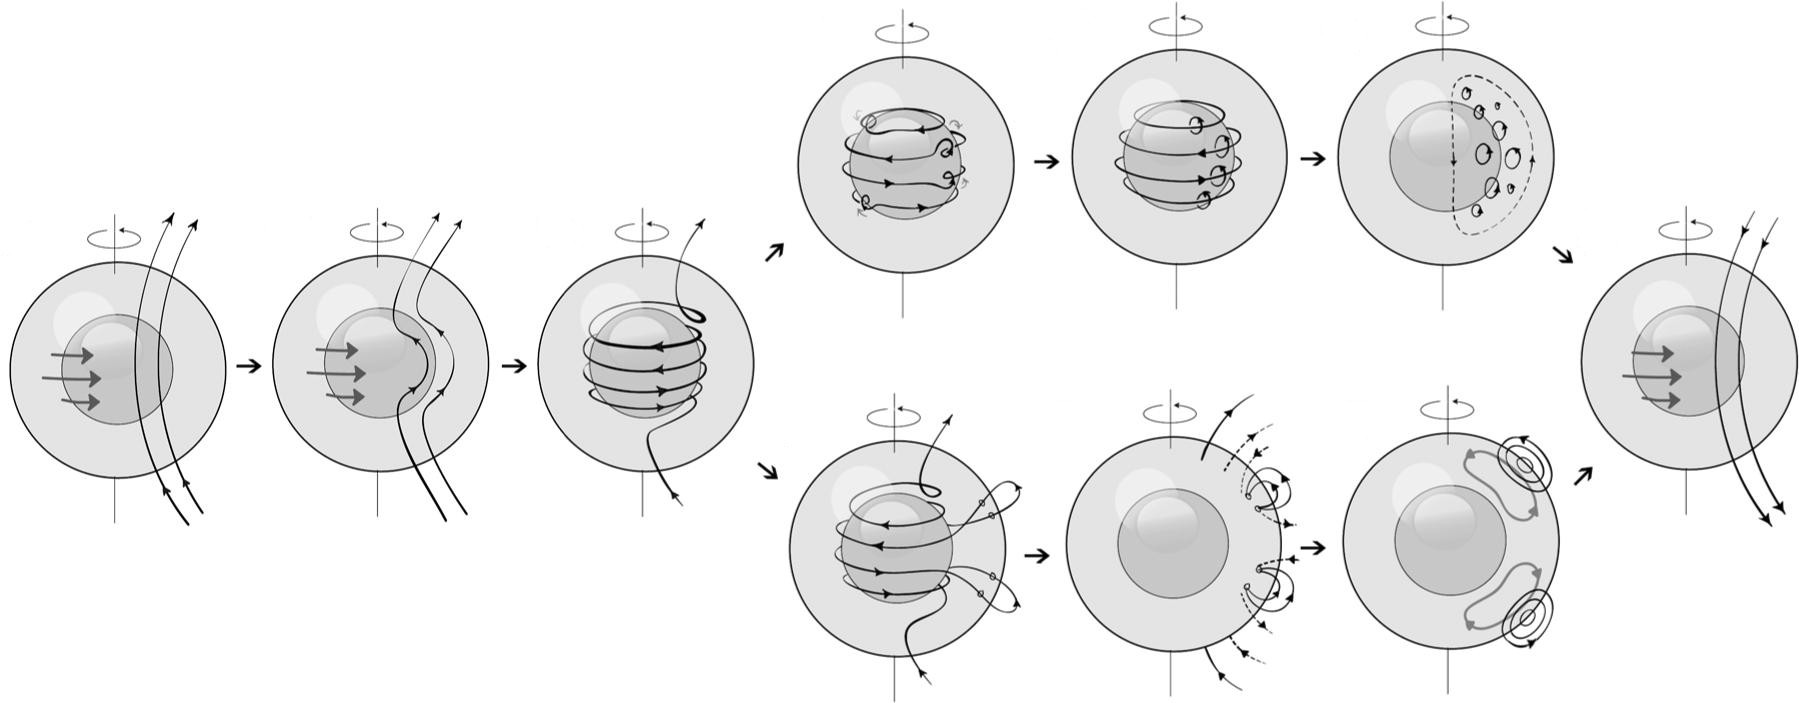
\includegraphics[width=0.95\columnwidth]{sun_dynamo.jpg}
	\caption{Schematic diagram of the main processes that drive the changes to the Sun's magnetic field. Staring from a poloidal field on the left, it is shown how the $\Omega$-effect generates a toroidal field. On the top we see a demonstration of the creation of small-scale poloidal magnetic fields, the $\alpha$-effect. On the bottom we see a demonstration of the Babcock-Leighton mechanism, diffusion and meridional flows. Finally, on the right we see the recovery of a poloidal field with opposite polarity. Adapted from \citet{sanchez_mean-field_2014}.}
	\label{fig:dynamo}
\end{figure}

The recovery of the poloidal field is not as straightforward. To recover a poloidal with opposite polarity, $P(-)$, there are two main schools of thought, as shown in Figure~\ref{fig:dynamo} \citep{sanchez_mean-field_2014}. One is based on the role of cyclonic turbulence and can be described by mean-field electrodynamics \citep{charbonneau_dynamo_2020}. Due to the influence of the Coriolis force, helical motions lift and twist the magnetic field, known as the $\alpha$-effect \citep{charbonneau_dynamo_2020}. The degree of twist can produce sources of poloidal field and through the combination of many small, accumulating elements, we get the generation of a new poloidal field with opposite polarity \citep{charbonneau_dynamo_2020}. Another mechanism is the Babcock-Leighton model \citep{babcock_topology_1961, leighton_transport_1964} whereby tilted bipolar regions of magnetic field undergo diffusion and cross-equatorial reconnection. Through the action of diffusion and meridional flows, poloidal flux is advected to the poles which creates a new poloidal field with opposite polarity \citep{sheeley_surface_2005, charbonneau_dynamo_2020}. There is debate in the literature about which mechanism dominates the recovery of the poloidal field.

%is a poleward transport of flux by diffusion and the meridional flow is responsible for the reversal of the polar field polarity after a toroidal field (see equation~\ref{eq:solar_cycle_dynamo}) \citep{sheeley_surface_2005, charbonneau_dynamo_2020}.
%helical twisting of toroidal fieldlines by the Coriolis force
%... ... ... is the $\alpha$-effect, but the details of how this effect works in the Sun is less well understood \citep{hathaway_solar_2015}. Helical motions that lift and twist the magnetic field which are important in the $\alpha$-effect \citep{babcock_topology_1961} and result from such processes as: (i) turbulence and mean-field electrodynamics; (ii) the Babcock-Leighton mechanism; (iii) hydrodynamical and magnetohydrodynamical instabilities (see \citet{charbonneau_dynamo_2020} for a complete review). This underpins the re-creation of a poloidal field with the same polarity as the toroidal field, $P(-)$. 
%"(d) and (e) show the effect of cyclonic turbulence on former toroidal fields, creating small-scale secondary poloidal magnetic fields - the α-effect. Averaged, they result in a net electromotive force generating a new large-scale poloidal field(f), closing the first half part of the magnetic cycle with a new poloidal field (g), with opposite polarity than the initial one. (h)represents the beginning of the Babcock-Leighton mechanism: toroidal flux tubes buoyantly rise to the surface forming sunspots, tilted bipolar regions. In (i), the fields from the bipolar regions diffuse and reconnect with each other and with the polar fields. The resulting poloidal flux is advected by meridional circulation to the poles (j), generating the final large-scale poloidal field in (g)." 
%"Turbulent motions associated with the Coriolis force, in turn, twist the toroidal field, generating a new component of the poloidal field and thus maintaining the solar cycle (Parker 1955). This latter process is known as the mean-fieldα-effect, and unlike the Ω-effect, is far from being totally understood, as well as the preferred place for its action. It is also known that the Lorentz force back-reaction of strong magnetic field inhibits turbulence, so the conventional α-effect would not lead to great effectiveness in regenerating the poloidal field in a dynamo within a strong magnetic field regime (Cattaneo and Hughes 1996). Other mechanisms, like interface dynamos, would overcome this problem, for the αΩ process would occur in the stably stratified layer comprising the tachocline (Parker 1993). Alternatively, the Babcock-Leighton mechanism may have an important role on the poloidal field regeneration. Differently from the meanα-effect, the Babcock-Leighton mechanism relies on the diffusion of the sunspots magnetic field, operating at the solar surface (Babcock 1961, Leighton 1969). However, the mechanism behind sunspot formation remains elusive (e.g. Guerrero and Käpylä (2011)), making it difficult to specify the exact nature of the Babcock-Leighton process in a model. In addition, magnetic pumping at the base of the convection zone provides an interesting complement to the Babcock-Leighton scenario (e.g. Guerrero and Gouveia Dal Pino (2008))."
%Bill's comments: "One explanation is offered by proponents of the flux-transport dynamo. But there is another explanation based on the role of cyclonic turbulence, and the so-called "alpha" effect (in which twists of magnetic field from the Coriolis effect combine in such a way as to give a large-scale change in field orientation)"
%my old polar drift comments: Poleward transport of following-polarity-flux by diffusion and the meridional flow is responsible for the reversal of the polar field polarity after a toroidal field (see equation~\ref{eq:solar_cycle_dynamo}) \citep{sheeley_surface_2005, charbonneau_dynamo_2020}.


These processes repeat with each cycle from poloidal-to-toroidal field and back to a poloidal field with opposite polarity (i.e. $P(+)\rightarrow T\rightarrow P(-)$), in $\sim11$~years. Therefore, it takes $\sim22$~years for the full magnetic cycle, the Hale cycle, to regenerate a poloidal field with the same polarity (i.e. $P(+)\rightarrow ...\rightarrow P(+)$).

The earliest observations of solar activity and the solar cycle were of sunspots, which date back to over 2000 years ago \citep{clark_interpretation_1978}. Sunspots are dark regions of concentrated, active magnetic flux which cross the photosphere. The earliest observation of solar-cycle variability associated with sunspots was by \citet{schwabe_sonnenbeobachtungen_1844}, who found that annual observations of sunspot groups, over a duration 18~years from 1826--1844, showed a cyclic behaviour, with a period of about 10 years.

Following this discovery \citet{wolf_mittheilungen_1856, wolf_extract_1859} acquired daily observations of \glspl{ssn} and extended the records as far back as 1749 \citep{hathaway_solar_2015}. This used a method of estimating the number of individual sunspots and sunspots groups; these \glspl{ssn} have since been used to monitor the solar activity cycle \citep{wolf_extract_1859, wolf_abstract_1861}. However, recently, a new, standard time-series of the \gls{ssn} has been generated to reconcile various discrepancies between different observers \citep{clette_preface_2016,clette_new_2016}: the \gls{issn}, which part of the \gls{silso} by the Royal Observatory of Belgium \citep{silso_world_data_center_international_2020}. These \glspl{ssn} are shown in Figure~\ref{fig:ssn}. Each activity cycle has unique characteristics and the \glspl{ssn} have been used to measure the properties of the cycles, for sunspot observations dating back to the year $\sim1750$.

\begin{figure}[ht!]
	\centering
	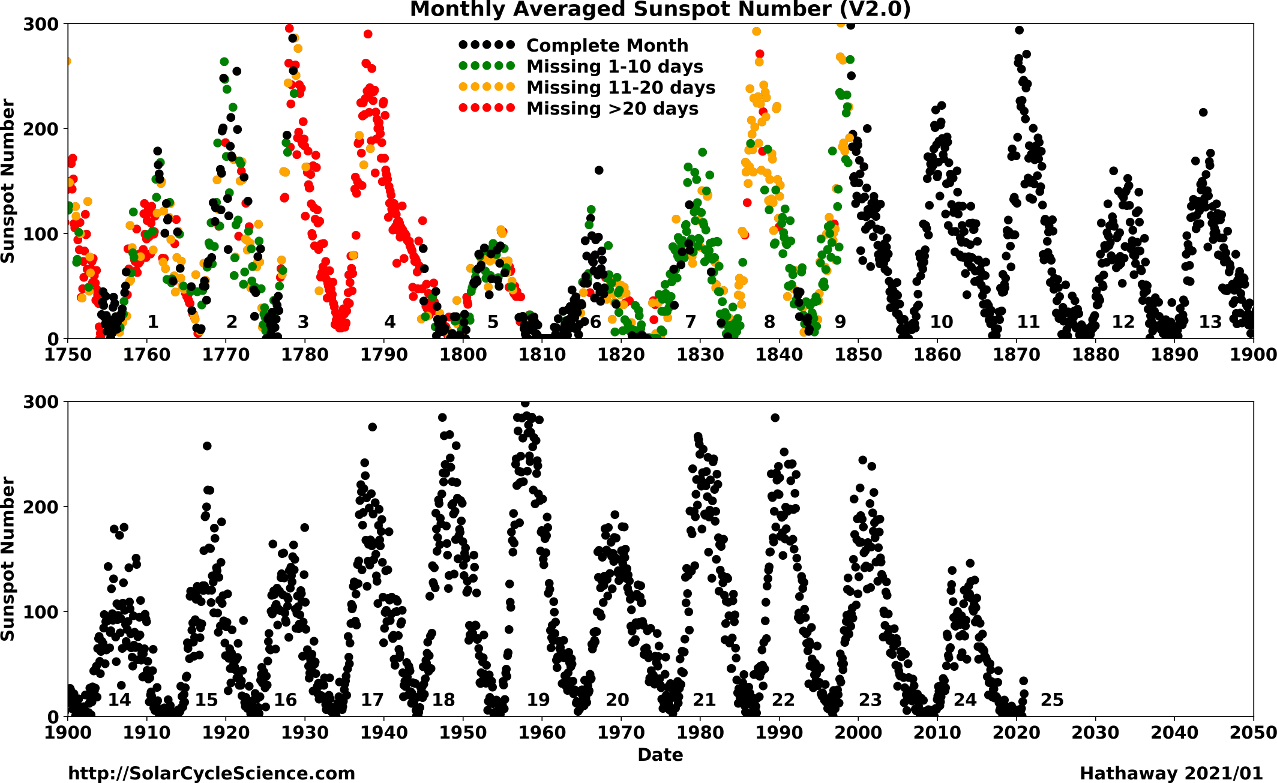
\includegraphics[width=\columnwidth]{SSN_monthly_landscape.png}
	\caption{Monthly averaged sunspot number since 1750 \citep{hathaway_solar_2017}. Black points indicate a full month of data, and then a traffic light system is in place to represent data quality, i.e. green for a near-complete month of data, amber for near 50\% duty cycle, and red for a very low data duty cycle.}
	\label{fig:ssn}
\end{figure}

Observations of sunspots in the 17th Century allowed astronomers to accurately measure the rotation of the Sun's surface, which they observed to be slightly under four weeks \citep{casanovas_early_1997, casas_solar_2006, luminet_reception_2017}. These early observations also showed that sunspots did not appear at latitudes higher than $\sim29^{\circ}/30^{\circ}$ \citep{casanovas_early_1997}. Later, it was confirmed that regions of strong surface magnetic activity were not distributed uniformly over the solar surface and also that the Sun exhibited a latitude-dependent differential surface rotation \citep{lee_cyril_1858}. %At the start of each cycle spots appear at latitudes above about $20^{\circ}-25^{\circ}$. 

As the solar cycle evolves the range of latitudes displaying sunspots decreases and the typical latitude of spots slowly drifts towards the equator, with a zone of avoidance near the equator \citep{hathaway_solar_2015}. This behaviour was first noticed by \citet{carrington_observations_1863} and is known as Sp\"{o}rer's Law of Zones, illustrated by the ``Butterfly Diagram" \citep{maunder_spoerers_1903, maunder_note_1904}, such as the one shown in Figure~\ref{fig:butterfly}.

\begin{figure}[ht!]
	\centering
	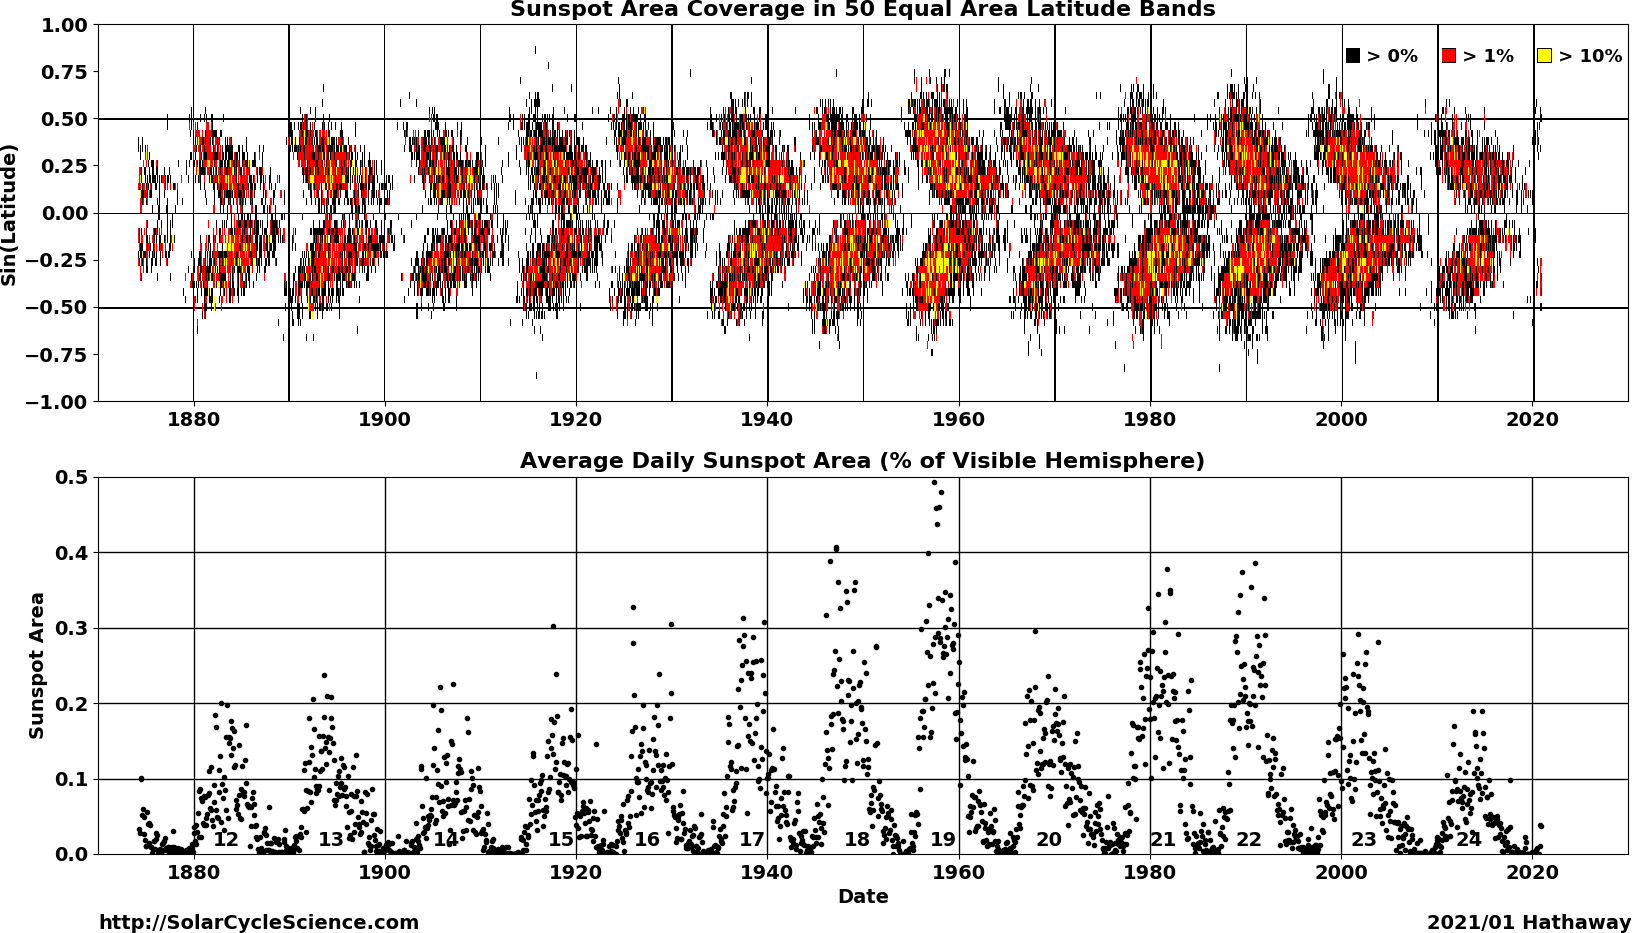
\includegraphics[width=\columnwidth]{ButterflyDiagram.png}
	\caption{Top panel: shows the latitudinal distribution of sunspots over time (also known as a ``Butterfly Diagram") and the colour of the points depict the area of the disc. Bottom panel: shows the average daily area of sunspots on the visible solar disc. Taken from \citet{hathaway_solar_2017}.}
	\label{fig:butterfly}
\end{figure}

In the first half of the 20th Century, it was discovered that sunspot groups in both hemispheres were tilted with respect to the Sun's equator, such that the leading spots (i.e. leading in the sense of the direction of rotation) exist closer to the equator than the following spots. This was first published by \citet{hale_magnetic_1919} but later defined as Joy's law. Furthermore, the degree of tilt varies with latitude, with a larger tilt at higher latitudes, and also with the solar cycle \citep{hathaway_solar_2015}. In addition, sunspots groups have opposite polarities in the Northern and Southern hemispheres, and the polarity changes from cycle-to-cycle. This effect is known as Hale's Polarity Law \citep{hale_law_1925}.

With the invention of the magnetograph \citep{babcock_solar_1953}, the Sun's magnetic field was probed further and it was found that sunspots were a characteristic of a larger phenomenon. It was discovered that sunspots are a small part of larger \glspl{ar} of magnetic field, which may be both \glspl{bmr} or \glspl{umr} \citep{babcock_suns_1955}.

Joy's law implies that the tilt of \glspl{bmr} systematically places the leading-polarity-flux at a lower latitude than the following-polarity-flux \citep{hathaway_solar_2015}. It is believed that there is a cancellation of leading-polarity flux on the opposite hemisphere near the equator \citep{dasi-espuig_sunspot_2010}. %Poleward transport of following-polarity-flux by diffusion and the meridional flow is responsible for the reversal of the polar field polarity after a toroidal field (see equation~\ref{eq:solar_cycle_dynamo}) \citep{sheeley_surface_2005, charbonneau_dynamo_2020}.

In very modern literature, the definition of the solar activity cycle has started to deviate away from counting sunspots and instead tracking the magnetic activity bands over the full, 22-year, Hale cycle \citep{leamon_termination_2018, leamon_timing_2020}. The existence of a ``Terminator" has been found, which marks the hand-over from one solar cycle to the next \citep{mcintosh_deciphering_2014, mcintosh_what_2019}. The terminator is defined as the abrupt annihilation or cancellation event of the oppositely polarized magnetic activity bands at the solar equator \citep{mcintosh_what_2019}. By employing the Hilbert transform on different proxies of the solar cycle, \citet{leamon_timing_2020} demonstrated a robust method to identify and predict the signature of terminators. The method has since been used to map severe space weather events to a ``solar cycle phase clock" \citep{chapman_quantifying_2020} and forecast the properties of Solar Cycle 25 \citep{mcintosh_overlapping_2020}. There exists some uncertainty about terminators in the solar physics community; the evidence presented so far suggests this method is robust, but will ultimately be tested with the evolution of Solar Cycle 25.


As discussed, the solar activity cycle exhibits a clear periodicty of approximately 11~years; however, there exist other, short-term periodicities in the solar activity cycle (see \citet{hathaway_solar_2015} for a review). The most prominent other feature in the solar activity cycle is an $\sim2$-year periodicity which manifests as a double peak in the maximum of \gls{ssn}, known as the Gnevyshev gap \citep{gnevyshev_corona_1963, gnevyshev_11-years_1967}. It was thought that this phenomenon was due to a superposition of sunspots from both hemispheres, slightly out of phase, but it was later confirmed that the Gnevyshev gap occurs in each hemisphere separately \citep{norton_solar-cycle_2009}. The cause of the Gnevyshev effect remains an open question \citep{hathaway_solar_2015}.

Finally, it has been suggested that long-term variations exist in the solar activity cycle, which consist of grand maxima and grand minima, which have led to the events such as the Maunder minimum (circa 1650--1700) and the Dalton minimum (circa 1790--1820). However, there is little evidence to support this long-term, cyclic variation \citep{hathaway_solar_2015}.

%[any discussion on peculiarities, such as large minima, i.e. maunder minimum, and recent extended deep minimum of cycle 23/24...?]


%%%%%%%%%%%%%%%%%%%%%%%%%%%%%%%%%%%%%%%%%%%%%%%%%%%%%%%%%%%%%%%%%%%%%%%%
\subsection{Features of Solar Activity}

There are many features that can be observed across the electromagnetic spectrum as a result of solar activity. In addition, with the advent of the magnetograph, solar activity can also be observed with direct measurements of the Sun's magnetic field, at different spatial scales. Many of these features are used widely in the literature as proxies of the solar activity cycle. Here we discuss these features and their properties.

\glsresetall 
{}
\subsubsection*{Active Regions}

An \gls{ar} has been defined as all \textit{observable} magnetic phenomena that appear preceding, during, and following the birth of sunspots, including electromagnetic and \gls{sep} emission \citep{kiepenheuer_structure_1968}. However, more generally, they appear when strands of magnetic flux emerge into the visible atmosphere from the solar interior.% and through the surface of the Sun. 

\citet{van_driel-gesztelyi_evolution_2015} recently proposed a new and more accurate definition of \glspl{ar}:

\begin{quote}
	\textit{the totality of observable phenomena in a 3D volume represented by the extension of the magnetic field from the photosphere to the corona, revealed by emissions over a wide range of wavelengths accompanying and following the emergence of strong twisted magnetic flux (i.e. kG).}% The simplest \glspl{ar} have bipolar magnetic field configurations, but \glspl{ar} may be built-up by several bipoles emerging in close succession.}
\end{quote}

This definition does not hinge on the appearance of a sunspot, which is important as not all \glspl{ar} produce spots \citep{van_driel-gesztelyi_evolution_2015}, and clearly defines their conditions and features. \glspl{ar} comprise of features in the photosphere, chromosphere, and corona; they typically appear as bipolar regions, obeying Hale's law, Joy's law, and Sp\"{o}rer's Law, and display a wide range of sizes and lifetimes. In addition, \glspl{ar} are typically confined to the specific `active' bands of latitude, between $\pm40^{\circ}$ \citep{harvey_solar_2001}.

The \glspl{ar} which produce sunspots are typically 10--100~Mm in size and have lifetimes on the order of several months \citep{zwaan_solar_1981, schrijver_photospheric_1994, canfield_solar_2001, van_driel-gesztelyi_evolution_2015}. However, it has been observed that \glspl{ar} exist with lifetimes in the range of days--months \citep{schrijver_solar_2008}. It is generally accepted that the lifetimes of \glspl{ar} depend approximately linearly on their size and strength \citep{canfield_solar_2001, schrijver_solar_2008}. The end of an \gls{ar} is determined by the dispersal of the magnetic flux by convective motion, differential rotation, meridional flows, and magnetic reconnection \citep{canfield_solar_2001}.


There are several other features that arise out of \glspl{ar}, such as: faculae, plages, and networks. Faculae are bright spots visible in the photosphere that appear bright at the limb but are nearly invisible at disc centre. They arise due to small magnetic flux tubes creating pores in the photosphere \citep{solovev_structure_2019}. If the flux tubes are small enough, they are heated by horizontal radiation transfer and the walls appear brighter than the surrounding area, which is known as the `hot-wall' model \citep{spruit_pressure_1976, keller_origin_2004}. Plages are bright regions in the solar chromosphere and are the chromospheric counterparts of faculae \citep{pillet_active_1997}. Networks are a product of the decaying remnants of \glspl{ar}, the merging and cancelling of mixed polarity fields in and around \glspl{ar}, and ephemeral regions -- often referred to as the `salt and pepper' field \citep{martin_identification_1988}.


\glsresetall 
{}
\subsubsection*{Ephemeral Regions}

A short-lived class of \glspl{ar} exists, known as \glspl{er} due to their short lifetimes.  \glspl{er} have sizes typically less than 20~Mm, lifetimes of a few hours, and produce no sunspots \citep{harvey_solar_2001}.

\glspl{er} emerge rapidly and it is possible that thousands of \glspl{er} emerge over the entire solar surface within a 24-hour period \citep{harvey_solar_2001}. There has been some disagreement in the literature on the temporal evolution of \glspl{er} with contradictory statements regarding whether the occurrence of \glspl{er} follows the activity cycle \citep[see][]{harvey_properties_1993, hagenaar_ephemeral_2001, vieira_evolution_2010}. However, some studies show compelling evidence that \glspl{er} are correlated with the solar activity cycle \citep[see e.g.][and references therein]{vieira_evolution_2010,chaplin_sensitivity_2019}. It was also shown that \glspl{er} follow the solar activity cycle but with a slight shift in phase compared to the sunspot minimum \citep{harvey_ephemeral_1973, martin_ephemeral_1979}.

Unlike \glspl{ar}, \glspl{er} are spatially located all over the solar disc \citep{harvey_solar_2001}. Furthermore \glspl{er} at high latitudes have been interpreted to be the first emergence of bipolar regions associated with the onset of a new solar cycle. Despite these differences, it has been reported that it is difficult to differentiate between large \glspl{er} and small \glspl{ar} \citep{harvey_solar_2001}.



\glsresetall 
{}
\subsubsection*{Sunspots}

As discussed above, sunspots have been used for centuries as a proxy for solar activity. Sunspots are dark regions on the disc of concentrated magnetic field. The convective heat flow is disrupted due to the magnetic field, therefore leaving the spots cooler than the surrounding photosphere \citep{solanki_sunspots_2003, hathaway_solar_2015}. Sunspots can sometimes appear in isolation; however, sunspots are generally found in groups, obeying Hale's law, Joy's law, and Sp\"{o}rer's Law. Each sunspot
is characterised by a dark, central core, called the \textit{umbra}, and a halo, called the \textit{penumbra} \citep{howard_sunspot_2001, solanki_sunspots_2003}. Sunspot groups are an important photometric counterpart of \glspl{ar} as the locations of extreme solar activity such as flares and \glspl{cme}.

The sizes of sunspots can vary substantially from diameters of around 2000~km, for the smallest sunspots, up to 60~Mm or more \citep{howard_sunspot_2001,solanki_sunspots_2003}. The lifetimes of sunspots range from minutes to months \citep{howard_sunspot_2001, solanki_sunspots_2003} and \citet{howard_sunspot_2001} states that more than half of sunspots have lifetimes $<2$~days, $90\%$ of sunspots have lifetimes $<11$~days, and it is rare for sunspots to have lifetimes of more than a few months. The lifetime increases linearly with maximum size, following the Gnevyshev-Waldmeier rule \citep{gnevyshev_notitle_1938, waldmeier_ergebnisse_1955}. The largest spots are generally the survivors of large sunspot groups, appearing as a single spot at least in the later stage of their lifetime \citep{howard_sunspot_2001}.

The equatorward drift of sunspots is a well-known characteristic of their evolution during the solar cycle. Sunspots emerge in active latitudes at around $\sim25-30^{\circ}$, and as the cycle progresses the mean latitude of the spots in each hemisphere steadily decreases. The number of sunspots varies with time with more spots observed during solar maximum and fewer observed at solar minimum (see Fig.~\ref{fig:ssn}). As such, the sunspot number is the most commonly used proxy for solar activity \citep{hathaway_solar_2015} and the \gls{issn} is the most widely used data set due to the length of the available record \citep{hathaway_solar_2015}. 

\glspl{ssn} are preserved and disseminated by the \gls{wdc} \gls{silso} of the Royal Observatory of Belgium \citep{silso_world_data_center_international_2020} and are provided as the daily \gls{ssn}, monthly averages, yearly averages, and the box-car smoothed \gls{ssn}. The standard smoothing is a 13-month \gls{cma} and the solar cycle maxima and minima are usually defined in terms of the smoothed \gls{ssn} \citep{hathaway_solar_2015}.


%\glsresetall 
%{}
\subsubsection*{10.7 cm Flux}

The 10.7~cm solar flux (F$_{10.7}$) is the disc-integrated radio emission from the Sun at a wavelength of 10.7~cm (in a 100~MHz-wide band centred on 2800~MHz) \citep{tapping_limits_1994,tapping_107_2013}. It is one of the most widely used indices of solar activity, alongside the \gls{ssn}, and the F$_{10.7}$ measure of solar activity has advantages over the \gls{ssn} in that it is completely objective \citep{hathaway_solar_2015}.

The F$_{10.7}$ comprises of Bremsstrahlung emission from the chromosphere and corona as well as over sunspots, where the magnetic fields are sufficiently strong to produce bright, compact sources from thermal, free–free electron gyroresonances \citep{tapping_origin_1990, tapping_107_2013}. However, the dominant component of the F$_{10.7}$ originates in the low corona \citep{tapping_origin_1990}.

The first observations were made in 1946 and have been recorded consistently since 1947 \citep{covington_solar_1969, tapping_107_2013}. The data can be acquired from the Laboratory for Atmospheric and Space Physics at University of Colorado \citep{lisird_solar_2019}.



\glsresetall 
{}
\subsubsection*{Solar Eruptions}
Solar flares are energetic, eruptive events which occur in the region of \glspl{ar} and complex sunspot groups \citep{hathaway_solar_2015}. The first reported solar flare was in 1859, the largest known flare to-date, the Carrington event \citep{carrington_description_1859}.

Solar flares follow the solar activity cycle, with more flares occurring at solar maximum, which is likely because during these times there are more \glspl{ar} on the Sun which tend to be flare-producing \citep{gopalswamy_corona_2010, hathaway_solar_2015}. However, there is a general propensity for more flares to occur during the declining phase of a sunspot cycle \citep{hathaway_solar_2015}.

\glspl{cme} are manifestations of concentrated solar activity and are associated with the significant release of plasma and accompanying magnetic field ejected from the corona. \glspl{cme} are often associated with solar flares but can also occur in isolation, in the absence of a flare \citep{hathaway_solar_2015}.

\glspl{cme} were first discovered in the early 1970s via spacecraft observations and have since routinely been observed \citep{hathaway_solar_2015}. A database of the properties of all \glspl{cme} observed since 1996 by the \gls{soho/lasco} instrument exists in the \gls{soho/lasco} catalogue\footnote{\url{https://cdaw.gsfc.nasa.gov/CME_list/}} \citep{yashiro_catalog_2004, gopalswamy_soholasco_2009}. 

Similarly to flares, the frequency of \glspl{cme} follow the solar activity cycle, with more \glspl{cme} occurring at solar maximum \citep{gopalswamy_corona_2010} and is therefore correlated with the \gls{ssn} \citep{webb_solar_1994}. In addition, physical properties of \glspl{cme} such as average speed, size, and the location of ejection from the Sun, etc. also vary with the solar activity cycle \citep{yashiro_catalog_2004}.



\subsubsection*{Total Magnetic Flux}

Individual elements of the magnetic field contribute to the large-scale field and determine the Sun's global magnetic dipole moment and the strength of the field in interplanetary space  \citep{lockwood_doubling_1999, solanki_evolution_2000}. The total, unsigned, magnetic flux is the amount of flux leaving the Sun and entering the heliosphere, i.e. the combination of \gls{ar}, \gls{er}, and open magnetic flux \citep{lockwood_doubling_1999}. The strength of the total magnetic flux and its main components has been shown to vary with the solar activity cycle \citep{solanki_secular_2002, vieira_evolution_2010, chaplin_sensitivity_2019}. \citet{vieira_evolution_2010} showed that the respective contributions to the total flux during maximum activity are approximately in the ratio 0.1:0.8:0.1, for \glspl{ar}, \glspl{er}, and open flux, while the ratios during minimum activity are approximately 0.5:0.4:0.1, for \glspl{ar}, \glspl{er}, and open flux. %The total magnetic flux is a useful indicator of solar activity and allows for the estimation of the magnetic conditions of the quiet Sun \citep{vieira_evolution_2010, chaplin_sensitivity_2019}.



\glsresetall 
{}
\subsubsection*{The Solar Mean Magnetic Field}

The \gls{smmf} is the mean \gls{los}, signed magnetic field when observing the Sun-as-a-star \citep{scherrer_mean_1977, scherrer_mean_1977-1, garcia_integrated_1999}. The \gls{smmf} is surprisingly a non-zero measurement of the imbalance of opposite magnetic flux polarities observed on the full, visible disc of the Sun \citep{svalgaard_suns_1975}, and its amplitude is observed to vary with the solar activity cycle.

The literature on \gls{smmf} observations spans several decades; however, the origin of the \gls{smmf} remains an open question in solar physics. We give a comprehensive review of the morphology of the \gls{smmf} in Section~\ref{sec:SMMF_intro}, since the analysis and interpretation of \gls{smmf} data collected by the \gls{bison} is presented in detail in that chapter.




\glsresetall 
{}
%%%%%%%%%%%%%%%%%%%%%%%%%%%%%%%%%%%%%%%%%%%%%%%%%%%%%%%%%%%%%%%%%%%%%%%%
%%%%%%%%%%%%%%%%%%%%%%%%%%%%%%%%%%%%%%%%%%%%%%%%%%%%%%%%%%%%%%%%%%%%%%%%
%%%%%%%%%%%%%%%%%%%%%%%%%%%%%%%%%%%%%%%%%%%%%%%%%%%%%%%%%%%%%%%%%%%%%%%%
\section{Space Weather}\label{sec:intro_SW}

\subsection{Background}
Space weather is defined as \citep{cannon_extreme_2013}:

\begin{quote}
	\textit{variations in the Sun, solar wind, magnetosphere, ionosphere, and thermosphere, which can influence the performance and reliability of a variety of space-borne and ground-based technological systems and can also endanger human health and safety.}
\end{quote}

Space weather phenomena have been observed over hundreds of years, mainly through observations of the aurorae, but its impacts are slowly becoming more tangible in modern civilisation, as we grow reliant on electronics \citep{beggan_ground_2018}. 

%Within the heliosphere t
There are two main sources of space weather: (i) those that are solar in nature and (ii) those whose origins are external to the solar system but penetrate into the heliosphere. Space weather manifests itself broadly in three ways:

\begin{enumerate}
	\item{Electromagnetic radiation, which is generally linked with an enhancement in the output of the Sun's spectrum.}
	
	\item{Magnetic fields/plasma, which can cause disturbances in the \gls{imf} and solar wind, and the Earth's magnetosphere.}
	
	\item{Energetic charged particles, which refer to ionising charged particles and ions.}
\end{enumerate}

The nature of their arrival and the resulting impact of these space weather phenomena at Earth depends on their type and energy. Space weather is the resultant product from solar storms -- magnetic disturbances on the Sun leading to large bursts of energy release and short-term heliospheric effects -- and the general chronology of events was outlined by \citet{cannon_extreme_2013}:

\begin{enumerate}
	\item{Storms begin with the evolution of one or more complex sunspot groups and \glspl{ar} on the solar surface.}
	
	\item{Within \glspl{ar}, one or more solar flares occur and the electromagnetic radiation is detected on Earth within approximately 8~minutes.}
	
	\item{\glspl{sep} are released and are measured at Earth, both using satellites and ground-based detectors, within approximately 15~minutes. \glspl{sep} continue to arrive over a period of several hours--days.}
	
	\item{A \gls{cme} occurs and propagates outwards, arriving at a distance of 1~AU within $\sim$15--72~hours. The impact on Earth depends on the \gls{cme} speed, how close it passes to Earth, and the orientation of the magnetic fields, with southward magnetic field generating the most severe geomagnetic storms because of its interference with Earth's northward magnetic field resulting in reconnection at the magnetopause.}
	
\end{enumerate}

The largest documented space weather event since modern records began occurred in 1859, the solar super storm known as the ``Carrington event" \citep{carrington_description_1859}. The available measurements of this event are limited to geomagnetic field perturbations, as well as eye witness accounts of solar brightening and aurorae \citep{cannon_extreme_2013}. However, recently cosmonuclide measurements from ice cores have been used to learn about the properties of the Carrington event \citep{riley_probability_2012}.%and it is believed that the large solar flare around this period exceeded class X10 \citep{riley_probability_2012}.

Since the beginning of the space age there have been no other super storms, however there have been large storms that have affected the infrastructure and caused a significant economic impact. The consensus is that another storm of the Carrington event level is inevitable and could significantly impact society. There is a view that a Carrington-like event may occur again in a period of 250 years with a confidence of $\sim$95\% and within a period of 50 years with a confidence of $\sim$50\% \citep{cannon_extreme_2013}; however, it is stressed that these figures should be interpreted with care. It was suggested by \cite{riley_probability_2012} that a Carrington-like event may occur with $\sim$ 12\% probability between 2012--2022 and later in 2012 a large storm occurred, missing Earth, but it strongly interacted with the STEREO-A satellite \citep{russell_very_2013}. This near miss highlights that Carrington-level events are a real threat to society and that we need a method of predicting their occurrence, arrival, and impact.



\subsection{Impacts of Space Weather}
\label{sw_impacts}
Space weather is an increasingly tangible threat to modern infrastructure and society, due to the increasing reliance on electronic technology. In 2011 space weather was added to the UK National Risk Assessment for the first time, and the subsequent National Risk Register in 2012 \citep{bis_space_2015} where it has remained to-date \citep{hm_government_national_2020}. At the time of writing this thesis, space weather risk was rated as a medium severity/high likelihood risk, at the same level as emerging infectious diseases, poor air quality, and heatwaves (see Figure~\ref{fig:UK_Risk_reg}) \citep{cabinet_office_national_2017}.

\begin{figure}[ht!]
	\centering
	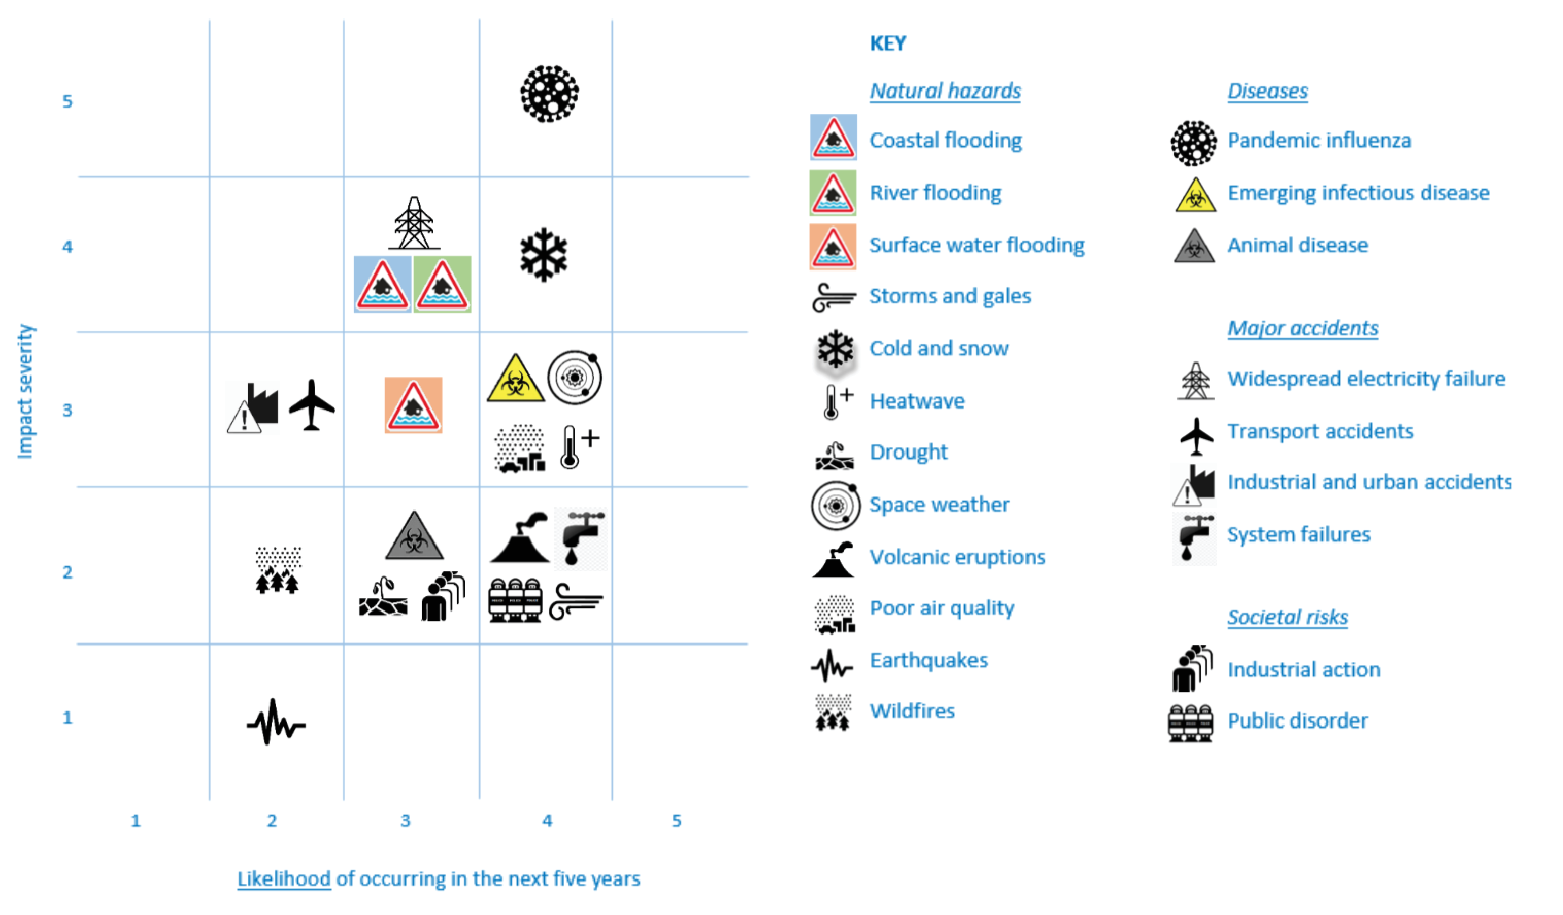
\includegraphics[width=\columnwidth]{UK_risk_register.eps}
	\caption{UK National Risk Register for hazards, diseases, accidents, and societal risks showing space weather as a medium-high risk \citep{cabinet_office_national_2017}}
	\label{fig:UK_Risk_reg}
\end{figure}

\vspace{1em}

An alarming aspect of Figure~\ref{fig:UK_Risk_reg} is that the likelihood of space weather events occurring in 5 years from 2017 was rated the same as pandemic influenza. Finishing this Ph.D. during a global pandemic highlights the importance of taking this risk register very seriously. We should learn from the global response to the COVID-19 pandemic and ensure that the world has a resolute plan to deal with the occurrence of a severe space weather event.

There are many ways that technological systems are impacted by space weather, both on or above ground, and Figure \ref{fig:space_weather_impacts} displays many of the key impacts that we know of \citep{beggan_ground_2018}. 


\begin{figure}[ht!]
	\centering
	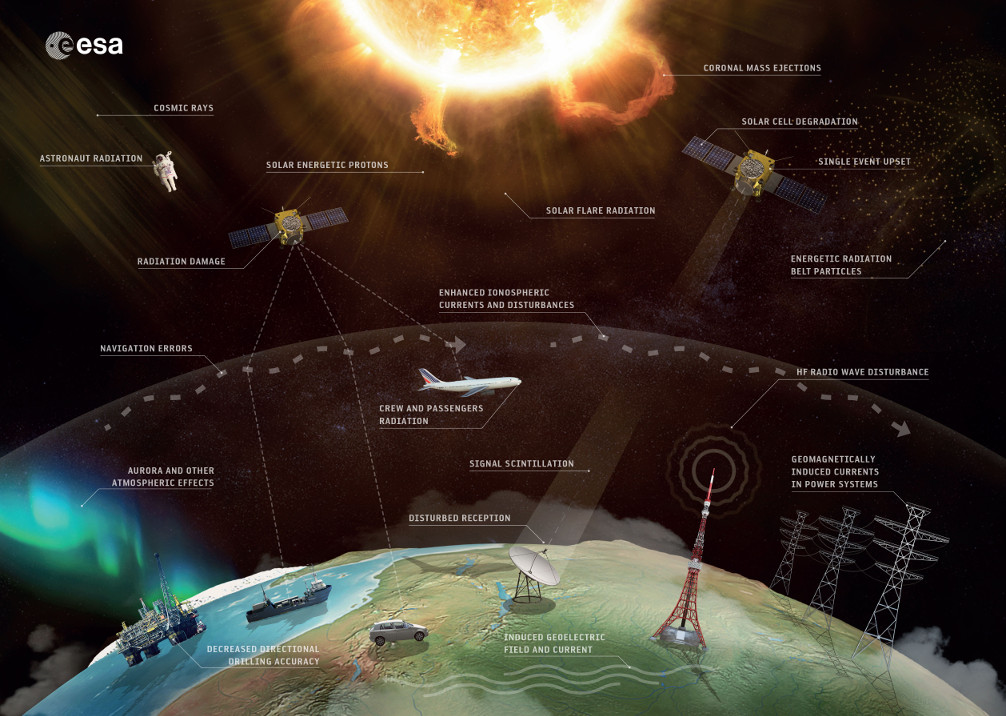
\includegraphics[width=\columnwidth]{Space_weather_effects_rescaled.jpg}
	\caption{The sources and effects of space weather. Impacts are shown including loss of telecommunications and GNSS, increased radiation levels, and ground induced currents (ESA/Science Office, \href{http://www.esa.int/spaceinimages/ESA_Multimedia/Copyright_Notice_Images}{CC BY-SA 3.0 IGO})}
	\label{fig:space_weather_impacts}
\end{figure}

\vspace{1em}

As far back as October 1841, it was reported that a solar storm was responsible for railway disruptions around Exeter, due to magnetic disturbances making it impossible to ascertain whether the onward line was clear, leading to delays \citep{nature_observations_1871}. 

It is possible for space weather events to induce geomagnetic storms that can cause damaging \glspl{gic} within large power grids, causing them to fail. Two such famous cases of \gls{gic} grid failures were in Quebec, Canada in 1989 which resulted in the failure of the Quebec-Hydro grid for 9 hours, and the city-wide black-out in Malm{\"o}, Sweden, during the Halloween storm in 2003 \citep{viljanen_european_2011, beggan_ground_2018}.

It was documented that in May 1967, the U.S. Air Force was close to engaging in conflict with its enemies -- during those politically tense times -- due to the misinterpretation of the effects of space weather \citep{knipp_may_2016}. \gls{srb} induced radio frequency interference was initially interpreted as surveillance jamming, an act of war. Fortunately, the U.S. had begun monitoring the space environment and were able determine that space weather was really the cause of the disruption, hence avoiding further conflict \citep{knipp_may_2016}. Furthermore, in more modern times, scintillation effects induced in the ionosphere affect \gls{gnss} communications which has a large societal effect due to our reliance on \gls{gnss} \citep{cannon_extreme_2013} as shown in Figure \ref{fig:space_weather_impacts}.

Solar storms are also responsible for creating sudden increases in ionising radiation which at typical flight altitudes can lead to the risk of malfunctions in aircraft microelectronic systems and unquantified radiation doses to passengers and crew \citep{cannon_extreme_2013}. In orbit, these conditions threaten the operation of satellites and the safety of manned space endeavours which is of particular concern with the current ambitions to return to the Moon and venture to Mars. 

There are even concerns that major storms could cause radiation increases at the Earth's surface, \glspl{gle}, which may cause malfunctions in microelectronics that are likely to be of increasing concern in the design of safety-critical systems \citep{cannon_extreme_2013}. 

Finally, a cost analysis estimated a present-day total U.S. economic cost for a super storm on the scale of the 1859 Carrington event \citep{homeier_solar_2013}. The cost estimated is heavily dependent on the duration of outages, the damages caused, and the availability of spare parts for repair; however they estimated the impact on the U.S. economy to be at around \$0.6--2.6 trillion \citep{homeier_solar_2013}. These figures show the large scale impact that space weather can have on the economy and that mitigation techniques to reduce this cost are of imperative necessity.

Due to the many ways that space weather can impact civilisation, and that it is predicted that there is a significant probably of the re-occurrence of large solar storms, it is easy to understand why space weather forecasting is becoming increasingly more necessary as a mitigation technique. 

The U.S. \gls{noaa} is the leading global space weather forecasting agency. The \gls{noaa} \gls{swpc} gathers data in real-time to describe the conditions of the Sun, heliosphere, magnetosphere, and ionosphere to understand the environment within the heliosphere and on Earth. With these data, the \gls{swpc} produces forecasts, warnings, and alerts available to inform anyone concerned and affected by space weather \citep{noaa_noaa_2018}. 

Following the addition of space weather to the UK risk register, the UK \gls{moswoc} opened in 2014 \citep{bis_space_2015}. \gls{moswoc} is mandated to produce daily space weather forecasts and is therefore developing a forecasting infrastructure using ground-based and satellite instrumentation to monitor space weather events. In addition, scientific research at \gls{moswoc} is carried out to better understand the physical processes involved in space weather phenomena to improve forecasting accuracy and lead-times; current forecasting enables prediction of \glspl{cme} impacting Earth to within only plus or minus six hours at best \citep{metoffice_space_2013}.

Forecasting and prediction is one aspect of the response to severe space weather events. We must also learn from the global response to the COVID-19 pandemic and ensure that upon the occurrence of a severe space weather event, suitable preplanning has been performed and a sufficient contingent action is planned.





\glsresetall 
{}
%%%%%%%%%%%%%%%%%%%%%%%%%%%%%%%%%%%%%%%%%%%%%%%%%%%%%%%%%%%%%%%%%%%%%%%%
%%%%%%%%%%%%%%%%%%%%%%%%%%%%%%%%%%%%%%%%%%%%%%%%%%%%%%%%%%%%%%%%%%%%%%%%
%%%%%%%%%%%%%%%%%%%%%%%%%%%%%%%%%%%%%%%%%%%%%%%%%%%%%%%%%%%%%%%%%%%%%%%%
\section{Cosmic Rays}\label{sec:intro_CRs}

\subsection{Background}
%The first accounts of measurement of \glspl{cr} date back to the 18th century, when scientists reported observations of spontaneous ionisation; however generally they were initially disregarded as they were believed to be due to imperfect experimental conditions \citep{montanus_observability_2017}. It was not until the late 19th and early 20th century that the nature of this spontaneous ionisation was understood to be caused by \glspl{cr}. 

\glspl{cr} are charged particles and atomic nuclei with energies spanning from 1~keV up to around $10^{21}$~eV, that encroach upon the Earth from all directions \citep{giacalone_energetic_2010}. It is understood that \glspl{cr} are composed of $\sim99\%$ of atomic nuclei and $\sim1\%$ electrons \citep{gaisser_cosmic_2016}; of the atomic nuclei $\sim87\%$ are protons, $\sim12\%$ are $\alpha$-particles, and a smaller contribution of $\sim1\%$ are heavier nuclei of around $\sim1\%$ \citep{grupen_astroparticle_2005, dunai_cosmic_2010, particle_data_group_review_2020}. \glspl{cr} mainly originate from outside the solar system, known as \glspl{gcr} \citep{particle_data_group_review_2020}. These \glspl{gcr} mostly come from within the Milky Way, although they are also expected to emanate from extra-galactic sources, in particular for \glspl{cr} with energies above $10^{18}$~eV \citep{aab_observation_2017}. Incoming low-energy \glspl{cr} ($\lesssim1$~GeV/nucleon) are modulated by the solar wind, which decelerates \glspl{gcr} and can even forbid lower-energy \glspl{gcr} from the inner solar system \citep{grupen_astroparticle_2005}. Consequently, there exists a strong anti-correlation between solar activity and the \glspl{gcr} flux \citep{particle_data_group_review_2020}.

Cosmic rays produced within the heliosphere are mostly of solar origin, known as \glspl{scr} or \glspl{sep}. These \glspl{scr} are generally of a lower energy than \glspl{gcr} and may be accelerated in the solar wind, by interplanetary shocks, or in solar eruptions (e.g. solar flares) \citep{giacalone_energetic_2010}. \glspl{scr} have typical energies on the order of magnitude of $\sim10^{1}$~keV--$1$~GeV \citep{chilingarian_galactic_2003, bruno_solar_2018}. Therefore, \glspl{pcr} associated with space weather events are generally of much lower energy than the background of \glspl{gcr}.

The intensity spectrum of \glspl{pcr} in the energy range from $10^9$~eV to $\sim10^{14}$~eV is given approximately by:

\begin{equation}
\label{eq:CR_flux}
I_N(E) = \frac{dN}{dE} \approx 1.8 \, \mathsf{x} \, 10^4 (E/1 \, \mathrm{GeV})^{-\alpha} \frac{\mathrm{nucleons}}{{\mathrm{m^2 \, s  \, sr \, GeV}}} \, ,
\end{equation}
%
where $E$ is the energy per nucleon (including rest mass energy) in GeV and $\alpha=2.7$ is the differential spectral index of the cosmic-ray flux \citep{particle_data_group_review_2020}. 

Figure~\ref{fig:CR_spec} shows a graphical representation of the \gls{cr} energy spectrum described by equation~(\ref{eq:CR_flux}). It shows the flux for a number of \gls{cr} species, over the energy range $10^{-1}$--$10^{6}$~GeV/nucleus, measured by several different experiments.

\begin{figure}[ht!]
	\centering
	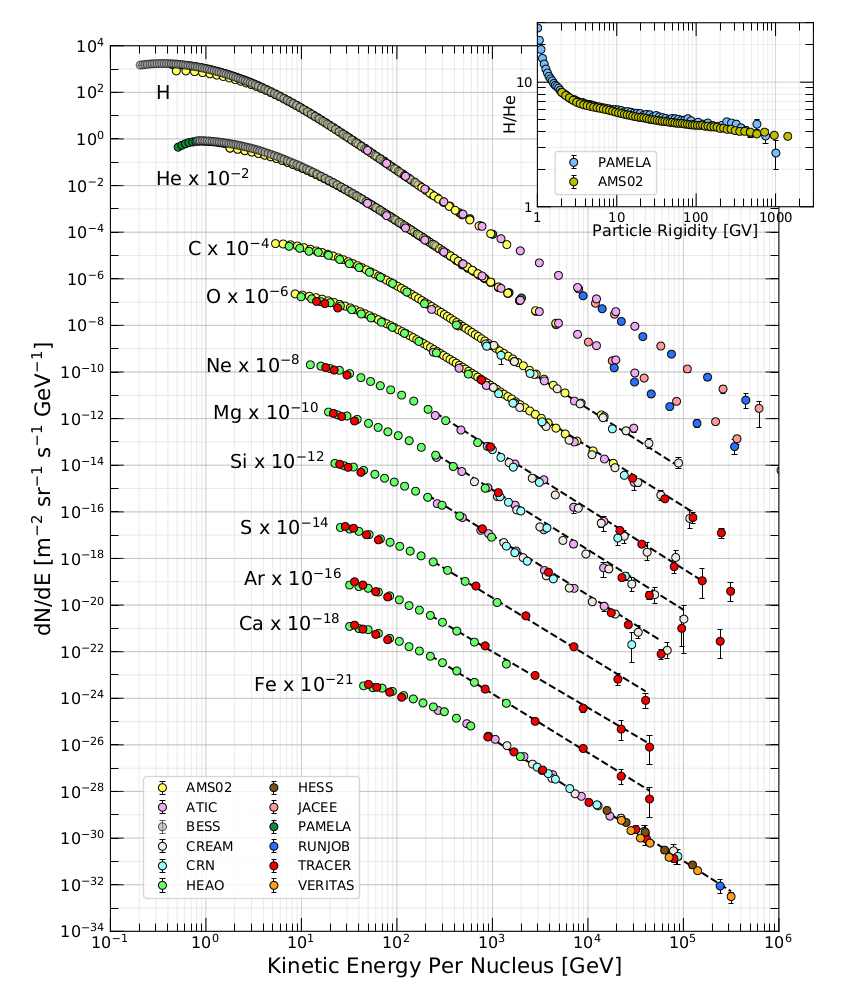
\includegraphics[width=0.8\columnwidth]{CR_spectrum.png}
	\caption{ Cosmic ray differential energy spectrum using data measured by several experiments. The inset shows the H/He ratio at constant rigidity \citep{particle_data_group_review_2020} }
	\label{fig:CR_spec}
\end{figure}

Beyond the x-axis range in Figure~\ref{fig:CR_spec}, the spectrum `knee' occurs (i.e. in the range $\sim10^{15}$--$10^{16}$~eV) where the spectral index is thought to increase to $\sim3$ \citep{particle_data_group_review_2020}. At even higher energies, in the region of the spectrum `ankle' ($\sim10^{18.5}$~eV) the spectral index reduces and the spectrum becomes less steep. This is in the regime of \glspl{uhecr} and the interaction between \glspl{gcr} and photons of the \gls{cmb} sets an upper limit on their energy, the \gls{gzk} limit \citep{particle_data_group_review_2020}. The \gls{gzk} limit implies that \glspl{cr} with energies exceeding $\sim5\times10^{19}$~eV must have originated from distances within a horizon of $\sim50$~Mpc, as otherwise their energy would have been reduced by the \gls{gzk} effect \citep{particle_data_group_review_2020}. 


Propagation of \glspl{cr} through magnetic fields depends on their gyroradius or Larmor radius \citep{particle_data_group_review_2020}. Therefore, a common description of \glspl{cr} uses a property called the {\textit{magnetic rigidity}} which is defined by:

\begin{equation}
\label{eq:rigidity}
R = r_L \, B \, c = \frac{p \, c}{Z \, e}
\end{equation}
%
where $r_L$ is the Larmor radius, $B$ is the magnetic field strength, $c$ is the speed of light, $p$ is the particle's momentum, $Z$ is the atomic number, and $e$ is the electron charge. The magnetic rigidity has units of Volts (V), or usually due to a large magnitude, Gigavolts (GV). The rigidity is used to describe \glspl{cr} as particles with different charges and masses have the same dynamics in a magnetic field if they have the same rigidity \citep{particle_data_group_review_2020}.



\subsection{Cosmic Rays in the Atmosphere}
\label{sec:air_shower}

\glspl{cr} in the interstellar medium traverse a very low-density medium, but experience a much denser environment when they reach the atmosphere. The typical nucleon mean free path (measured in units of $\mathrm{g}\,\mathrm{cm}^{-2}$) of protons in the atmosphere is approximately $90~\mathrm{g}\,\mathrm{cm}^{-2}$, which means the first interactions of \glspl{cr} occur in the upper layers of the atmosphere, at a height of $\sim15$--$20$~km \citep{grupen_astroparticle_2005}. %scale height used to calculate this, i.e. if X = X_0 exp(-h/H), where X is the atmospheric depth (g/cm2), X_0 is sea level atmospheric depth (1030 g/cm2), H is scale height (~8.5km), then rearranging finds h ~ 20km.

The \glspl{pcr} will predominantly interact with the atmospheric nuclei via strong interactions \citep{grupen_astroparticle_2005}. When \glspl{pcr} interact with atmospheric nuclei, the interaction leads to the production of a cascade of secondary particles. The secondary particles can also undergo interaction or decay, producing tertiary particles, and the process continues until the energies of all particles are insufficient to create new particles. If a concentrated, large number of secondary particles reach ground-level, the cascade of particles is called an \gls{as}, or an \gls{eas} for extremely high numbers of secondary particles, which can have a footprint area of several~km$^2$ \cite{fokkema_hisparc_2012, van_dam_hisparc_2020}]. The \gls{as} is often described as being a cone, with the base being the shower front and the apex being the primary \gls{cr}.

Hadronic cascade components (or the ``hard component" of \glspl{as}) are produced by \gls{cr} protons and nuclei interacting with atmospheric nuclei. This process typically produces lower energy protons, neutrons, pions, and kaons. In this thesis we are mostly interested in the muonic air shower development (see Section~\ref{sec:intro_HiSPARC}), so here we will focus on the development of the mesons in the \glspl{as}, as they predominantly produce muons. In Table~\ref{tab:meson_decay}, the most likely modes of decay for air shower mesons are shown with the branching ratio for each mode. In addition, the table shows the most likely decay modes of muons.


\begin{table}[ht!]
	\begin{center}
		\caption{ Most prominent decay modes of the mesonic components of CR air showers and of muons. Note: $K^-$ modes are charge conjugates of the decay modes below \citep{particle_data_group_review_2020}}
		\label{tab:meson_decay}
		\begin{tabular}{lc}
			\hline
			Decay mode & Branching ratio  \\
			\hline
			{$ \pi^{+} \, \rightarrow \, \mu^{+} \, + \, \nu_{\mu} $}	 &  $99.98770 \pm 0.00004 \%$ \\
			{$ \pi^{-} \, \rightarrow \, \mu^{-} \, + \, \overline{\nu_{\mu}} $}  &  $99.98770 \pm 0.00004 \% $ \\
			{$ \pi^{0} \, \rightarrow \, \gamma \, + \, \gamma $} &  $98.823 \pm 0.034 \% $ \\
			{$ \pi^{0} \, \rightarrow \, e^+ \, + \, e^-  \, + \, \gamma $} &  $1.174 \pm 0.035 \% $ \\
			{}  & {} \\
			{$K^+ \, \rightarrow \, \mu^{+} \, + \, \nu_{\mu}$}  &  $63.56 \pm 0.11 \% $ \\
			{$K^+ \, \rightarrow \, \pi^{+} \, + \pi^{0} $}  &  $20.67 \pm 0.08 \% $ \\
			{$K^+ \, \rightarrow \, \pi^{+} \, + \pi^{+} \, + \pi^{-}$}  &  $5.583 \pm 0.024 \% $ \\
			{$K^+ \, \rightarrow \, \pi^{0} \, + e^{+} \, + \nu_{e}$}  & $5.07 \pm 0.04 \% $ \\ 		 		 		 		
			{$K^+ \, \rightarrow \, \pi^{0} \, + \mu^{+} \, + \nu_{\mu}$}  &  $3.352 \pm 0.033 \% $\\ 		 		 		 		
			{$K^+ \, \rightarrow \, \pi^{+} \, + \pi^{0} \, + \pi^{0}$}  &  $1.760 \pm 0.023 \% $\\
			{}  & {} \\
			{$ \mu^{+} \, \rightarrow \, e^{+} \, + \, \nu_e \, + \, \overline{\nu_{\mu}} $}  &  $\sim 100\%$\\	
			{$ \mu^{-} \, \rightarrow \, e^{-} \, + \, \overline{\nu_e} \, + \, \nu_{\mu} $}  &  $\sim 100\%$\\	
			\hline
		\end{tabular}
	\end{center}
\end{table}


Due to the short lifetimes of pions and kaons, $\sim26$~ns and $\sim12$~ns, respectively \citep{particle_data_group_review_2020}, and depending on energy, they decay during their journey to ground-level. It is shown in Table~\ref{tab:meson_decay} that the most probable decay modes involve the production of muons. Muons are the most abundant charged particles at ground level \citep{particle_data_group_review_2020}; on average, the ground level muon flux is on the order of $\sim 70 \, \mathrm{m}^{-2}\,\mathrm{s}^{-1}\,\mathrm{sr}^{-1}$ \citep{cecchini_cosmic_2000, blackmore_terrestrial_2015, pereira_ground_2020, particle_data_group_review_2020}. Most muons are produced high in the atmosphere ($\sim15$~km) and lose about 2~GeV to ionization before reaching the ground and the mean energy of muons at the ground is $\sim4$~GeV \citep{particle_data_group_review_2020}.

%; hence when produced at low enough altitudes allowing enough time for these muons to reach ground, there is a large muon contingent at the ground level. At sea level the average kinetic energy of muons is approximately 4 GeV \citep{bartels_hisparc_2012}.

In addition to the hadronic component of an air shower, electron and photon constituents of cascades are called the electromagnetic component (or ``soft component"). These are typically initiated by electrons and photons under the processes of Bremsstrahlung \citep{grupen_astroparticle_2005},

\begin{equation}
\label{eq:bremss}
e \, \rightarrow \, e \, + \, \gamma \, ,
\end{equation}
%
or pair production \citep{grupen_astroparticle_2005},
%
\begin{equation}
\label{eq:pair_prod}
\gamma \, \rightarrow \, e^- \, + \, e^+ \, .
\end{equation}

Ionisation losses mean that electrons and positrons lose energy rapidly until they either annihilate or recombine with nuclei, and photons lose their energy by being either absorbed in scattering and/or the photoelectric effect. Therefore, most of the electrons, positrons,
and photons observed at ground level are produced from the decaying hadronic \gls{as} component and muon decay is the dominant source of low-energy electrons at ground level \citep{particle_data_group_review_2020}.

Finally, there is a minimum rigidity cut-off which implies that the energy of any \gls{pcr} must exceed a minimum energy to be able to initiate an \gls{as} or particle cascade and be measured at ground-level. This limit is dependent on the depth of the atmosphere above the detector, but is greatest at sea-level and decreases with increasing altitude. The minimum energy to be measured at sea-level is approx. $430$~MeV/nucleon \citep{dorman_theory_2004, dorman_experimental_2004, poluianov_gle_2017}.



\subsection{Cosmic Ray Detectors}

To observe \glspl{cr} there are many types of usable detectors, both ground-based and space-based \citep{schrijver_heliophysics_2010}; in this thesis we are mostly concerned with ground-based detectors of the \gls{as} hadronic component. The most common type of ground-based \gls{cr} detectors are \glspl{nm} and \glspl{md} which indirectly measure \gls{cr} particles through the secondary particles produced in \gls{cr} cascades. These two types of detector probe different energy ranges; \glspl{nm} generally observe \glspl{pcr} with energies $\sim$1--10~GeV and above, while \glspl{md} typically observe higher energy \glspl{pcr} with energies on the order of $\gtrsim10$~GeV \citep{kuwabara_real-time_2006, rockenbach_global_2014}.

\subsubsection*{Neutron Monitors}
The neutron monitor, invented by \cite{simpson_latitude_1948}, has been extensively used for \gls{cr} observations of the space environment \citep{clem_neutron_2000}. The \gls{nm} is an example of an ionisation detector whereby energetic neutrons encounter a nucleus within a gas, producing charged, secondary particles which in turn ionise the surrounding gas \citep{gloeckler_-situ_2010}.

The original ``IGY" \gls{nm} design made use of a paraffin reflector to trap slow neutrons within the detector, a producer material (typically lead) which multiplied the number of slow neutrons registered by the detector in order to amplify the signal, a moderator to further slow neutrons, and cylindrical proportional counters utilising BF\textsubscript{3} gas \citep{simpson_latitude_1948, simpson_cosmic_1953}. A schematic diagram of the detector is shown in Figure~\ref{fig:NMIGY}. %The proportional counter is essentially a gas-filled chamber with two electrodes; a potential difference between the electrodes attracts the ionised gas collecting positive and negative charge which results in charge appearing across a coupling capacitor \citep{schrijver_heliophysics_2010}. Following the discharge of the capacitor, the signal is then amplified and recorded through the back-end electronics \citep{simpson_latitude_1948, simpson_cosmic_1953}.

\begin{figure}[ht!]
	\centering
	\subfloat[Standard IGY]{{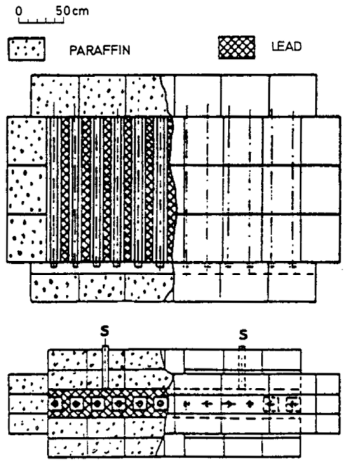
\includegraphics[width=0.36\columnwidth]{NM_IGY_rescaled.png} } \label{fig:NMIGY}}%
	\qquad
	\subfloat[6-tube NM64]{{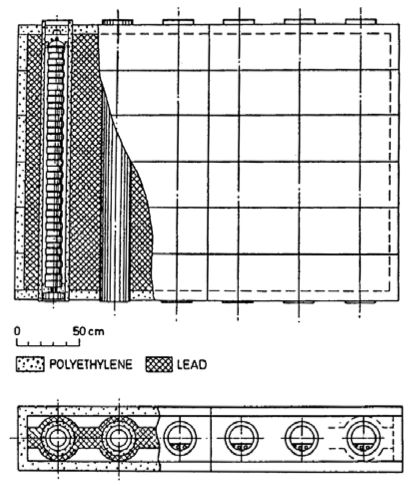
\includegraphics[width=0.36\columnwidth]{NM_64_rescaled.png} } \label{fig:NM64}}%
	\caption{Schematic diagrams of two NM configurations: (a) the original Simpson's 12-tube IGY NM is shown where the paraffin reflector is represented by the outer dotted blocks; the lead producer is represented by the cross-hatched section; the paraffin moderator is represented by the inner dotted blocks; finally the gas-filled proportional counters are denoted by the black circles/tubes. (b) the modern NM64 is shown on the right in its 6-tube configuration where the polyethylene reflector is represented by the outer dotted section; the lead producer is represented by the cross-hatched area; within the producer is a cylindrical polyethylene moderator denoted by the dotted ring; finally in the centre of each tube is a gas-filled proportional counter. In each figure the top schematic is a top-down drawing and the bottom is an end-on drawing. Taken from \citet{kang_characteristics_2012}.}
	\label{fig:NM}
\end{figure}

An improved ``NM64" \gls{nm} design is now the preferred detector type, which makes use of a polyethylene reflector, lead producer, polyethylene moderator, and \textsuperscript{10}BF\textsubscript{3} or \textsuperscript{3}He gas-filled cylindrical proportional counters \citep{kang_characteristics_2012}. A schematic diagram of the detector is shown in Figure~\ref{fig:NM64}. The new design provided an improvement over the IGY design by a factor of about 3.3 in the count rate per unit area of producer \citep{stoker_neutron_2000}; the choice of \textsuperscript{10}BF\textsubscript{3} gas or \textsuperscript{3}He gas does not significantly affect the detector performance \citep{kang_characteristics_2012}.



\subsubsection*{Muon Detectors}

Muon detectors are an example of a scintillation detector, whereby light emitted by atoms excited in a medium is collected and converted into an electrical signal. The scintillation medium can be solid, liquid, or gas; however solid scintillation detectors are attractive as they have a higher electron density \citep{gloeckler_-situ_2010}.

The general configuration of a \gls{md} is shown in Figure~\ref{fig:MD}. When an energetic particle passes through a scintillator material, some of the particle's energy is lost in ionising the scintillator material and the scintillator material releases photons. The light pipe directs the photons towards a \gls{pmt} where a cascade of electrons are produced and the resulting electrical signal is amplified and recorded through the back-end electronics.

\begin{figure}[ht]
	\centering
	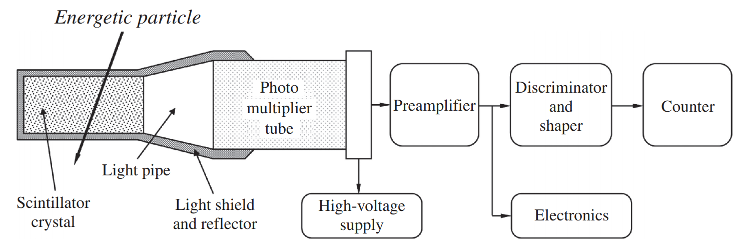
\includegraphics[width=0.7\columnwidth]{scintillator_rescaled.png}
	\caption{Schematic design of a typical scintillation muon detector with back-end electronics \citep{gloeckler_-situ_2010}}
	\label{fig:MD}
\end{figure}

Desirable properties of scintillator materials are a high conversion efficiency, transparency to the light that they emit, short fluorescent decay times, and spectral distributions suitable for photosensitive devices \citep{gloeckler_-situ_2010}. 

A range of different material types are used in scintillator detectors however the most common scintillator materials for \glspl{md} are organic scintillators consisting of aromatic hydrocarbons (the fluors) in a solid plastic solvent (the base) \citep{gloeckler_-situ_2010, fokkema_hisparc_2012}. Energetic particles traversing the scintillator excite the base rather than the fluor due to the low fluor density. The plastic base however has a low yield and is not transparent to its own scintillation light; thus the fluor is added to therefore increase the yield of this popular type of scintillator \citep{fokkema_hisparc_2012}.





\subsection{Cosmic Ray Observations of Solar Activity and Space Weather}

It has long been established that there exists an anti-correlation between \gls{gcr} intensity and the level of solar activity, over the $\sim11$-year period \citep{forbush_cosmic-ray_1958, parker_passage_1965, usoskin_correlative_1998, van_allen_modulation_2000}. We also see the 22-year Hale cycle manifesting in the \gls{gcr} intensity, as interchanging peaked and flat-topped cycles of \gls{gcr} intensity due to combination of solar activity and \gls{cr} transport processes \citep{aslam_solar_2012, thomas_22-year_2014}, as seen in Figure~\ref{fig:gcr_plot}. The effects of solar activity on \glspl{cr} observations are discussed in more details in the introduction to Chapter~\ref{chap:GCR_SSN_24}, since the analysis and interpretation of \gls{gcr} data is presented in detail in that chapter.
%The positively charged cosmic rays drift in from the heliospheric polar regions when the Sun's north polar field is directed outward (positive). When the Sun's north polar field is directed inward (negative) the positively charged cosmic rays drift inward along the heliospheric current sheet where they are scattered by corrugations in the current sheet and by magnetic clouds from CMEs. The negatively charged cosmic rays (electrons) drift inward from directions (polar or equatorial) opposite to the positively charged cosmic rays that are detected by neutron monitors.

\begin{figure}[ht!]
	\centering
	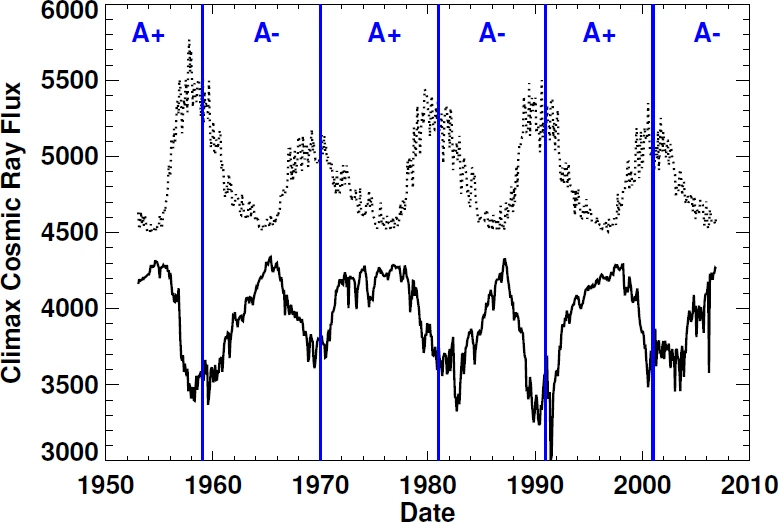
\includegraphics[width=0.95\columnwidth]{gcr.png}
	\caption{Cosmic ray flux measured at the Climax NM (solid line) and rescaled SSN (dotted line) taken from \citet{hathaway_solar_2015}. The vertical lines denote changes in the Sun's global magnetic field polarity, where: A$+$ indicates positive polarity at the North Pole; A$-$ indicates negative polarity at the North Pole.}
	\label{fig:gcr_plot}
\end{figure}

There have been many documented observations of space weather events using \gls{cr} detectors. The most notable types of \gls{cr} space weather effects are \glspl{fd} and \glspl{gle}; here we discuss the properties of each.

\subsubsection*{Forbush Decreases}\label{sec:intro_FDs}

Short-term decreases in the \gls{gcr} flux were first observed by  \citet{forbush_effects_1937} and therefore were later coined as \glspl{fd} or \glspl{fe}. \glspl{fd} are characterised by a sharp decrease in \gls{gcr} intensity over a period of several hours--days, followed by a gradual recovery taking place over several days--a week \citep{cane_coronal_2000, belov_forbush_2008, wawrzynczak_modeling_2010}, as shown in Figure~\ref{fig:FD_plot}.

\begin{figure}[htb!]
	\centering
	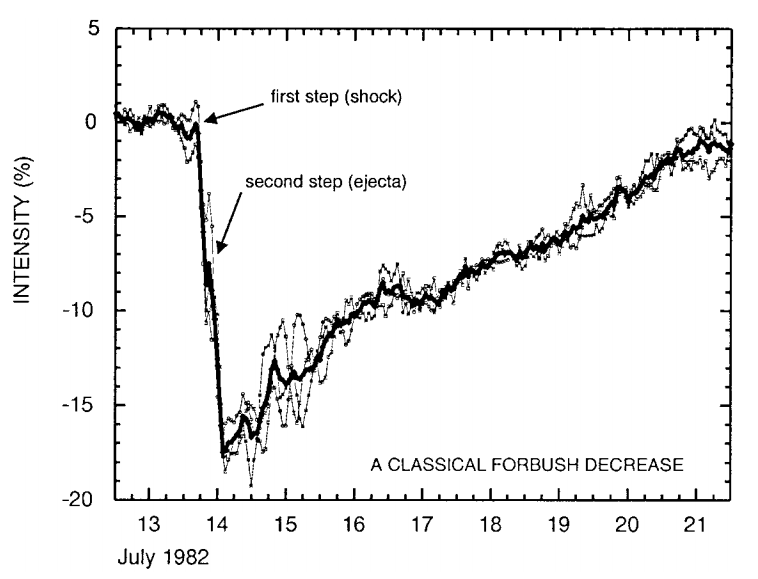
\includegraphics[width=0.75\columnwidth]{FD_plot.png}
	\caption{A two-step Forbush decrease measured at three NM stations, Deep River, Mt.Wellington, Kerguelen, in July 1982 \citep{cane_coronal_2000}. The thicker black line indicates the average of the count rates from the three stations. Arrows show the start of the two decreases caused by the shock and the ICME ejecta.}
	\label{fig:FD_plot}
\end{figure}

There are two \gls{fd} origins: one caused by \glspl{cir} \citep{dumbovic_forbush_2016}, and one caused by \glspl{icme} and the shocks they drive \citep{belov_forbush_2008}. The biggest \glspl{fd} (magnitudes $> 5\%$) are strictly associated with \glspl{icme} \citep{belov_what_2001}. Of the kind caused by \glspl{icme}, the majority are produced by \glspl{icme} with speeds in the range 400--1200~km~s$^{-1}$ \citep{lingri_forbush_2016}; the typical speed of the solar wind is, for slow solar wind, in the range 300--400~km~s$^{-1}$, and for fast solar wind, $\sim 750$~km~s$^{-1}$ \citep{owens_heliospheric_2013}. Previous literature has also shown that the type caused by \glspl{cir} produce recurrent, more symmetric, and lower-amplitude decreases \citep{dumbovic_cosmic_2012}, while the type caused by \glspl{icme} result in the more strongly asymmetric decreases as shown in Figure~\ref{fig:FD_plot} \citep{lockwood_forbush_1971, cane_coronal_2000, dumbovic_cosmic_2012}. In addition the \gls{icme}-driven \glspl{fd} typically result in a two-step \gls{fd}, where the first step of the decrease is due to the passage of the leading shock and the second step is due to the \gls{icme} itself, as shown in Figure~\ref{fig:FD_CME} \citep{cane_coronal_2000}.

\begin{figure}[ht!]
	\centering
	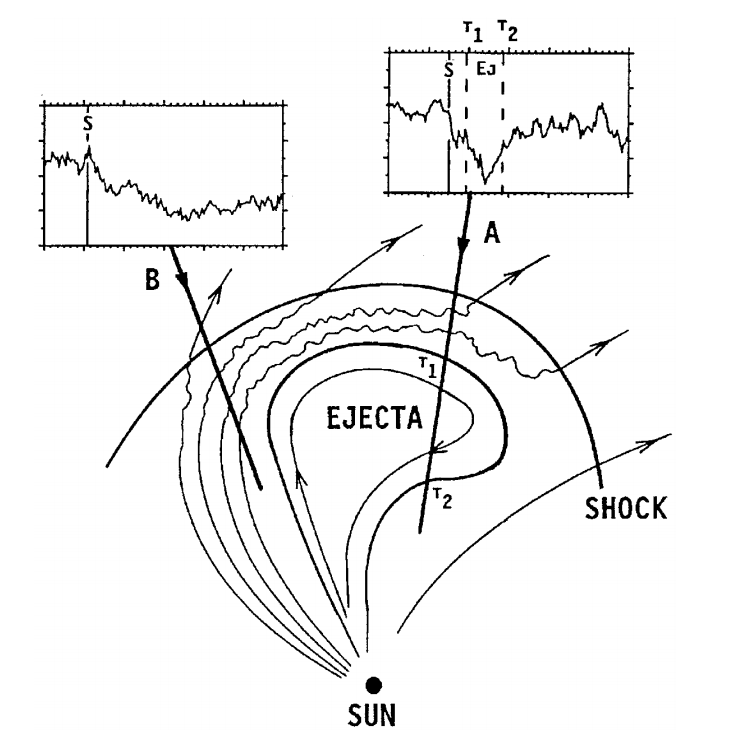
\includegraphics[width=0.75\columnwidth]{FD_CME.png}
	\caption{A schematic diagram of an ICME-driven FD taken from \citet{cane_coronal_2000}. It shows the different cosmic ray responses from two paths, indicated by A and B. A experiences the shock and ejecta, therefore experiencing a two-step FD; B only experiences the shock, therefore experiencing a single decrease. The time of shock passage is indicated by a solid, vertical line marked, S; the start and end times of ejecta passage are indicated by vertical, dashed lines marked T1 and T2, respectively.}
	\label{fig:FD_CME}
\end{figure}

\citet{lockwood_forbush_1971} showed that there is a rigidity dependence on the amplitudes of \glspl{fd}, which is approximately related to $R^{-\gamma}$, where the exponent ranges from $0.4\lesssim\gamma\lesssim1.2$. In addition, \citet{belov_what_2001, belov_coronal_2014} showed the magnitude of the \gls{fd} is proportional to the speed, mass, and width of the \gls{cme}. 


The \gls{feid}\footnote{\url{http://spaceweather.izmiran.ru/eng/dbs.html}} is a record of all the \glspl{fd} observed since the beginning of the \gls{gnmn} \citep{mishev_current_2020}. The total number of events is $\sim 7630$ during the epoch 1957--2020. Many studies have analysed observations of \glspl{fd} using these data and investigated their features, driving factors, and precursors; for an overview see: \citet{belov_what_2001, usoskin_forbush_2008, wawrzynczak_modeling_2010, rockenbach_global_2014, arunbabu_how_2015}.



\subsubsection*{Ground Level Enhancements}\label{sec:intro_GLEs}

Short-term increases in the \gls{gcr} flux were first observed in the 1940s and early 1950s, but it was not until after the largest recorded event, in September 1956, that these increases were defined as \glspl{gle} \citep{cramp_modelling_1996}. \glspl{gle} are the detection of an increased number of the highest-energy portion \cite[$> 500$~MeV,][]{kuwabara_development_2006} of \glspl{sep} arriving at Earth along lines of \gls{imf} that are accelerated following a solar eruptive event \citep{mccracken_high-energy_2012, poluianov_revisited_2017}. The \glspl{sep}, which cause \glspl{gle}, can cause serious damage to satellite electronics and are a hazard to air crew and astronauts; hence, the monitoring of these events are of importance for space weather forecasting. \glspl{gle} are characterised by a sharp rise in \gls{cr} intensity over a period of several minutes--hours, followed by a gradual decay taking place over several hours, as shown in Figure~\ref{fig:GLE_plot}. 

\begin{figure}[ht!]
	\centering
	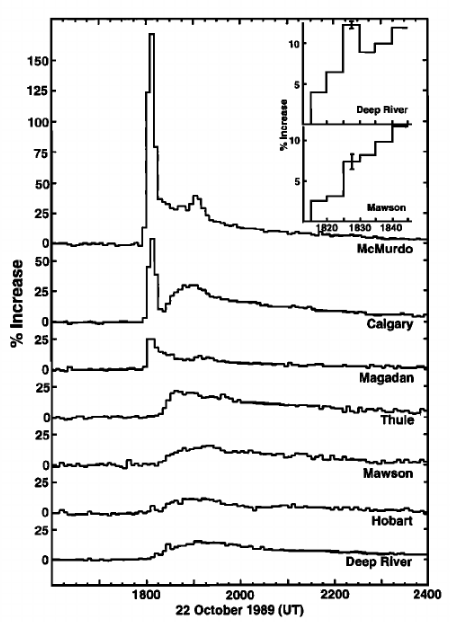
\includegraphics[width=0.75\columnwidth]{GLE_plot.png}
	\caption{A GLE measured at nine NM stations in October 1989, taken from \citet{cramp_j._l._october_1997}.}
	\label{fig:GLE_plot}
\end{figure}


\glspl{gle} result from energetic solar eruptions such as flares and \glspl{cme} \citep{mccracken_high-energy_2012}. The total number of \glspl{gle} observed to-date is low: there have been only 72. The \gls{gle} database\footnote{\url{https://gle.oulu.fi}} is a record of events, starting from \gls{gle} 5 (February 1956), since the beginning of the \gls{gnmn} \citep{usoskin_database_2016}. Many studies have discussed the observations of \glspl{gle}, investigating their features as well as the spectra and anisotropy of \glspl{pcr} that produce the \glspl{gle}; for an overview see: \citet{,shea_possible_1982, cramp_modelling_1996, belov_ground_2010, mccracken_high-energy_2012, strauss_pulse_2017,  mishev_first_2018}. \citet{strauss_pulse_2017} analysed the shapes of fourteen \glspl{gle} and showed the existence of a linear dependence between the rise ($\tau_r$) and decay ($\tau_d$) times which they empirically determined to be $\tau_d\approx3.5\tau_r$. In addition, the average decay time of \glspl{gle} as measured by \citet{strauss_pulse_2017} was $1.8^{+1.9}_{-1.3}$~hours.

The solar magnetic field is `frozen' into the solar wind plasma. As the Sun rotates, so do the \gls{imf} lines which forms an Archimedean spiral, the Parker spiral \citep{parker_dynamics_1958, parker_spiral_1976}. A curved field line connecting the Sun to the Earth stems from the western limb of the Sun, at a longitude of about $60^{\circ}$, which is known as the `garden hose' field line (see Fig.~\ref{fig:garden_hose}) \citep{duldig_ground_1993, hathaway_solar_2015}. Charged particles follow magnetic field lines and therefore \glspl{sep} that are accelerated in flares located near to the solar end of the `garden hose' field line usually arrive at Earth rapidly and have very sharp onsets \citep{duldig_ground_1993, andriopoulou_intense_2011}. This causes a strong anisotropy in the arrival directions of the early \glspl{sep} inducing \glspl{gle}, as shown in Figure~\ref{fig:GLE_plot}. The McMurdo, Calgary, and Magaden \gls{nm} stations observed an earlier \gls{gle} onset, with a high magnitude, than the other stations \citep{duldig_ground_1993, cramp_j._l._october_1997}. This shows that for a sufficiently anisotropic event, i.e. a \gls{gle} where \glspl{sep} are predominantly directed towards Earth, different stations at the same cut-off rigidity, but located at different longitudes, may respond differently.

\begin{figure}[ht!]
	\centering
	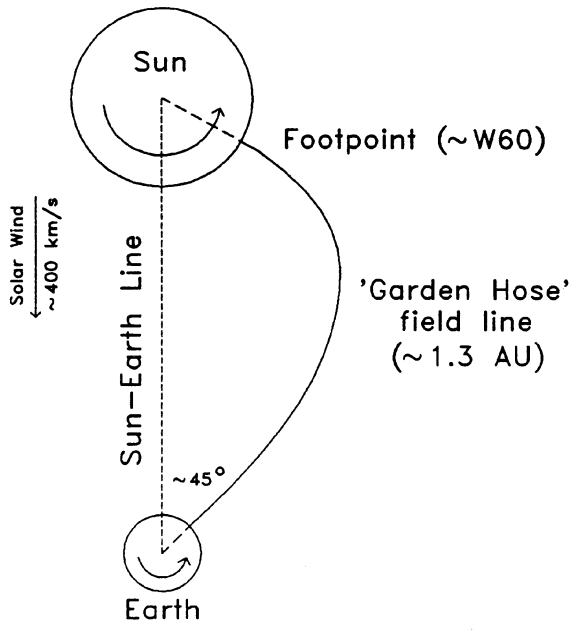
\includegraphics[width=0.75\columnwidth]{garden_hose.png}
	\caption{A schematic diagram of the `garden hose' field line taken from \cite{duldig_ground_1993}.}
	\label{fig:garden_hose}
\end{figure}

Conversely, \glspl{gle} associated with flares far from the `garden hose' field line are usually delayed in their arrival at Earth, due to having to cross magnetic field lines, and have more gradual increases to maximum intensity \citep{duldig_ground_1993}. Very few \glspl{gle} have originated far away from the base of the `garden hose' at the solar surface \citep{duldig_ground_1993, andriopoulou_intense_2011}.

Most \glspl{gle} are detected by multiple stations because of a low enough anisotropy \citep{strauss_pulse_2017,belov_global_2018} and in part due to their definition. The accepted definition of a \gls{gle} since the 1970s has been \citep{poluianov_gle_2017}: 

\begin{quote}
	\textit{a GLE event is registered when there are near-time coincident and statistically significant enhancements of the count rates of at least two differently located NMs.}
\end{quote}

However, recently a newer \gls{gle} definition has been adopted due to the increase in the number of \gls{nm} stations that are more sensitive to lower energy \glspl{cr} due to their high latitudes (i.e. in near-polar regions) or higher altitudes. It is a concern that these new \gls{nm} stations will classify many more \glspl{gle} than their near-sea-level counterparts, thus affecting the homogeneity of the current list of \glspl{gle} \citep{poluianov_gle_2017}. Therefore, the new \gls{gle} definition is as follows \citep{poluianov_gle_2017}: 

\begin{quote}
	\textit{a GLE event is registered when there are near-time coincident and statistically significant enhancements of the count rates of at least two differently located neutron monitors, including at least one neutron monitor near sea-level and a corresponding enhancement in the proton flux measured by a space-borne instrument(s).}
\end{quote}

The new definition also invoked the introduction of a sub-\gls{gle} class, defined as \citep{poluianov_gle_2017}:

\begin{quote}
	\textit{a sub-GLE event is registered when there are near-time coincident and statistically significant enhancements of the count rates of at least two differently located high-elevation neutron monitors and a corresponding enhancement in the proton flux measured by a space-borne instrument(s), but no statistically significant enhancement in the count rates of neutron monitors near sea level.}
\end{quote}


Finally, a \gls{gle} real-time alarm system was developed by \citet{kuwabara_real-time_2006, kuwabara_development_2006}, using data from \glspl{nm} and \glspl{md}, which has been shown to provide the earliest alert for the onset of \gls{sep}-driven space weather events. They showed their alerts provide a warning up to an hour earlier than the storm onset. Furthermore, they also show that through utilising the \gls{gnmn}, monitoring precursory anisotropy, they can also issue warnings several hours ahead of near-Earth, in-situ satellite observations. They state that using both \glspl{nm} and \glspl{md} provides a dual energy range for observations, providing a more effective system.


\glsresetall 
{}
%%%%%%%%%%%%%%%%%%%%%%%%%%%%%%%%%%%%%%%%%%%%%%%%%%%%%%%%%%%%%%%%%%%%%%%%
%%%%%%%%%%%%%%%%%%%%%%%%%%%%%%%%%%%%%%%%%%%%%%%%%%%%%%%%%%%%%%%%%%%%%%%%
%%%%%%%%%%%%%%%%%%%%%%%%%%%%%%%%%%%%%%%%%%%%%%%%%%%%%%%%%%%%%%%%%%%%%%%%
\section{The HiSPARC Experiment}\label{sec:intro_HiSPARC}

%%%%%%%%%%%%%%%%%%%%%%%%%%%%%%%%%%%%%%%%%%%%%%%%%%%%%%%%%%%%%%%%%%%%%%%%
\subsection{Background}

The \gls{hisparc} is a scientific outreach project that was initiated in the Netherlands in 2002 \citep{bartels_hisparc_2012}. The \gls{hisparc} experiment has two main goals: the study of \gls{uhecr} for astroparticle physics research, and to serve as a resource to expose high school students to scientific research \citep{bartels_hisparc_2012}.

\gls{hisparc} is a global network of muon detectors spread across the Netherlands, Denmark, the UK, and Namibia. There are $\sim140$ stations in the \gls{hisparc} network \citep{van_dam_hisparc_2020} which have been uploading data for varying durations since 2005. The detection philosophy of \gls{hisparc} is to sample the footprints of \glspl{eas} using coincident triggers between scintillation detectors. The detectors at each station record muon counts and may be used for many scientific experiments, such as: reconstruction of the direction of a cosmic ray induced air shower, reconstruction of the energy of the air shower's primary particle, investigation between the atmospheric conditions and the number of cosmic rays observed, etc. A comprehensive review of the \gls{hisparc} experiment is provided by \citet{fokkema_hisparc_2012} and \citet{van_dam_hisparc_2020}.

The \gls{hisparc} network has predominantly been used to study \glspl{uhecr}, i.e. \glspl{pcr} with energies in excess of $\sim10^{14}$~eV. However, \citet{van_dam_probing_2020} used the \gls{hisparc} data to derive the \gls{cr} flux at sea level for \glspl{pcr} with energies between $10^{12}$--$10^{16}$~eV. Furthermore, \citet{fan_analysis_2018} provided a study into the anti-correlation between atmospheric pressure and the \gls{hisparc} data, as well as claiming to demonstrate the correlation between the daily-average of \gls{cr} events and solar activity proxies.



%%%%%%%%%%%%%%%%%%%%%%%%%%%%%%%%%%%%%%%%%%%%%%%%%%%%%%%%%%%%%%%%%%%%%
\subsection{HiSPARC Detector and Station Configuration}

As \gls{hisparc} was set up as an outreach programme for high schools, this impacted detector design \citep{fokkema_hisparc_2012, van_dam_hisparc_2020}. Resources are limited in schools and the detectors are usually financed by the participating high schools, colleges, and universities. In addition, students (accompanied by their teachers and local node support staff) are responsible for assembly and installation of their detectors, which are typically installed on the roofs of schools. Due to this, the detectors needed to be cheap, robust, and easily maintainable, therefore the scintillation detector was selected for the \gls{hisparc} network.

Scintillators consist of materials that emit light when charged particles pass through them with sufficient energy to ionise the scintillator material. The total light produced is proportional to the number of charged particles, and can be collected by a \gls{pmt}. Each \gls{hisparc} detector utilises a plastic scintillator of dimensions $1000$~mm~$\times~500$~mm~$\times~20$~mm, providing a detection area of 0.5~$\mathrm{m}^2$. A vertically incident \gls{mip} has a most probable energy loss in 2~cm of the scintillation material of 3.51~MeV ($\equiv 1$ \gls{mip}) \citep{van_dam_hisparc_2020}.

The scintillator is glued to a triangular/`fish-tailed' light-guide (dimensions, base: 500~mm; top: 25~mm; height: 675~mm), and a light-guide adapter provides the optical interface between the square end of the light-guide and the cylindrical aperture of the \gls{pmt}. The configuration of a single \gls{hisparc} detector is shown in Figure~\ref{fig:HS_scintillator}. 

\begin{figure}[ht!]
	\centering
	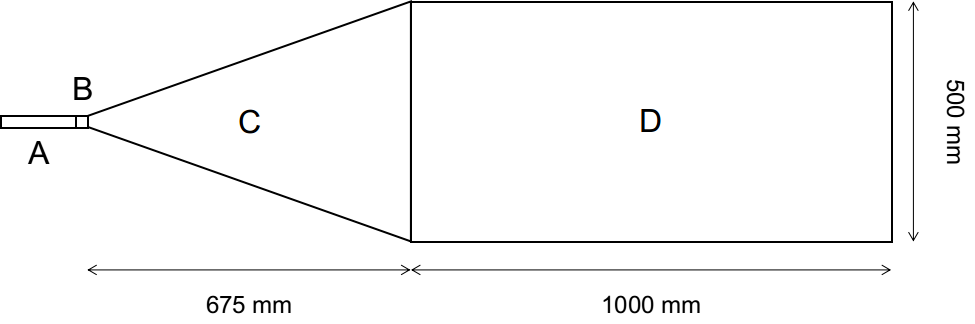
\includegraphics[width=0.75\columnwidth]{config.png}
	\caption{Schematic diagram of the HiSPARC scintillation detector. (A): PMT; (B): light-guide adaptor; (C): light-guide; (D): scintillator.}
	\label{fig:HS_scintillator}
\end{figure}

The scintillator is made of a material consisting of polyvinyltoluene as the base, with anthracene as the fluor, and the emission spectrum peaks at a wavelength of 425~nm \citep{fokkema_hisparc_2012, bartels_hisparc_2012}. The light-guide is made from \gls{pmma} and has a comparable refractive index to the scintillator (1.58 and 1.49, respectively), reducing refraction effects between the two materials \citep{van_dam_hisparc_2020}.

The \gls{pmt} used is an ETEnterprises 9125B model, with a 25~mm aperture,  blue-green sensitive bialkali photocathode, and 11 high-gain dynodes \citep{bartels_hisparc_2012,et_enterprises_data_2020}. The quantum efficiency of the \gls{pmt} used in the \gls{hisparc} detectors peaks at around 375~nm at 28\%, and at 425~nm the quantum efficiency is 25\% \citep{fokkema_hisparc_2012}. 

Each detector is wrapped in aluminium foil (thickness 30~$\upmu$m) and a black, vinyl material (thickness 0.45~mm), which is usually used as a pond liner, to ensure light-tight detectors and to reduce the noise level from stray photons \citep{van_dam_hisparc_2020}. In addition, each detector is placed inside its own a plastic roof box to again ensure that it is light-tight, and to also ensure that it is weather-proof, as the detectors are usually located on the roofs of schools, colleges, and universities.

The \gls{hisparc} detectors have, individually, a high muon-detection
efficiency close to $100\%$ \citep{fokkema_hisparc_2012, van_dam_hisparc_2020}, therefore they are capable of observing any muons that traverse them. A \gls{hisparc} station combines either 2 or 4 detectors, to observe coincident muons (`events'), and typical configurations of each are shown in Figure~\ref{fig:HS_station_layouts}. The separation between detectors varies from station-to-station and this influences the measurable footprint and hence the observable \glspl{pcr}.


\begin{figure}[htbp!]
	\centering
	\subfloat[Two-detector station configuration]{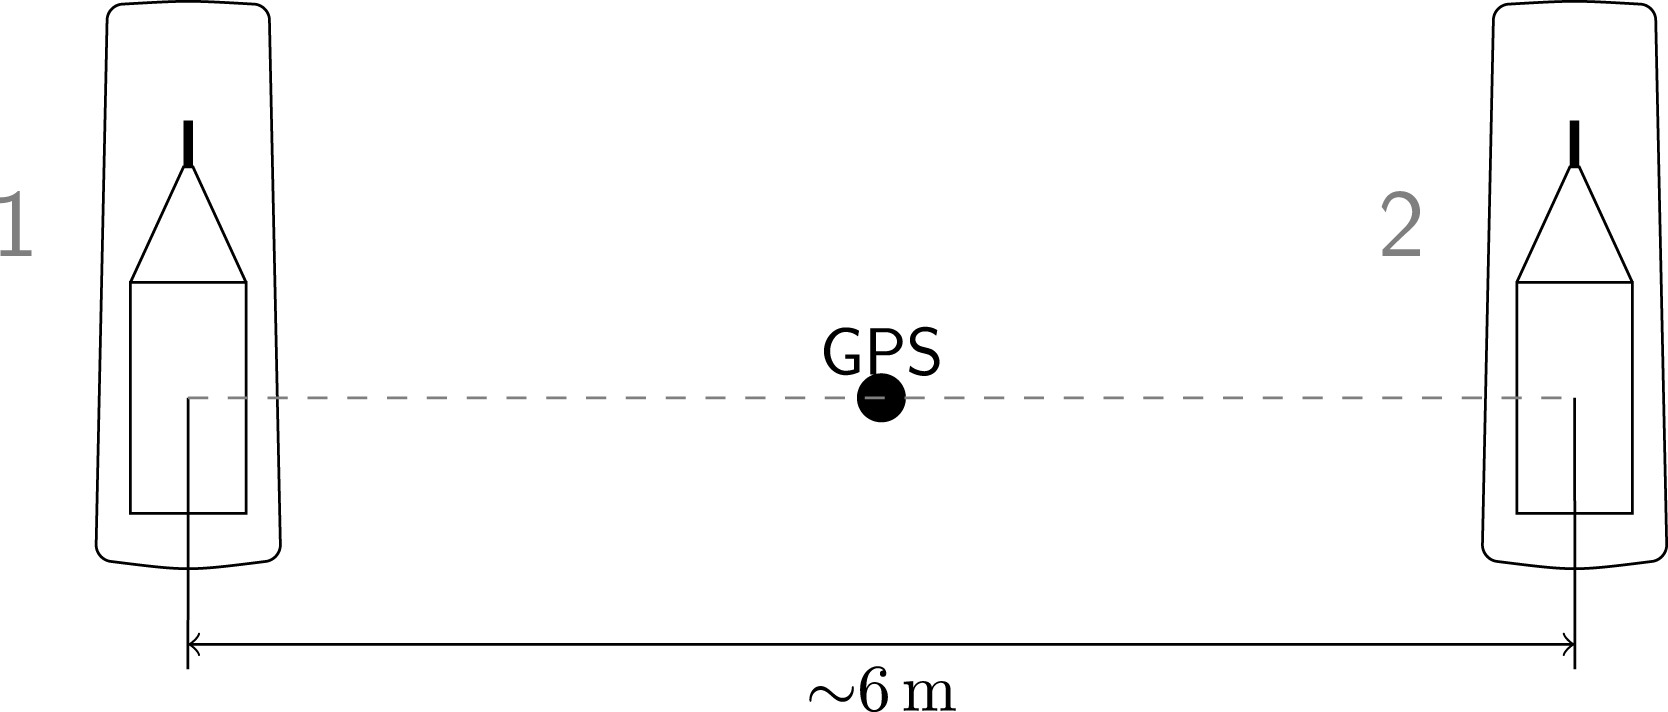
\includegraphics[width=0.5\columnwidth]{HS_2det.jpg}} 
	\qquad
	\subfloat[Four-detector station configuration (triangle arrangement)]{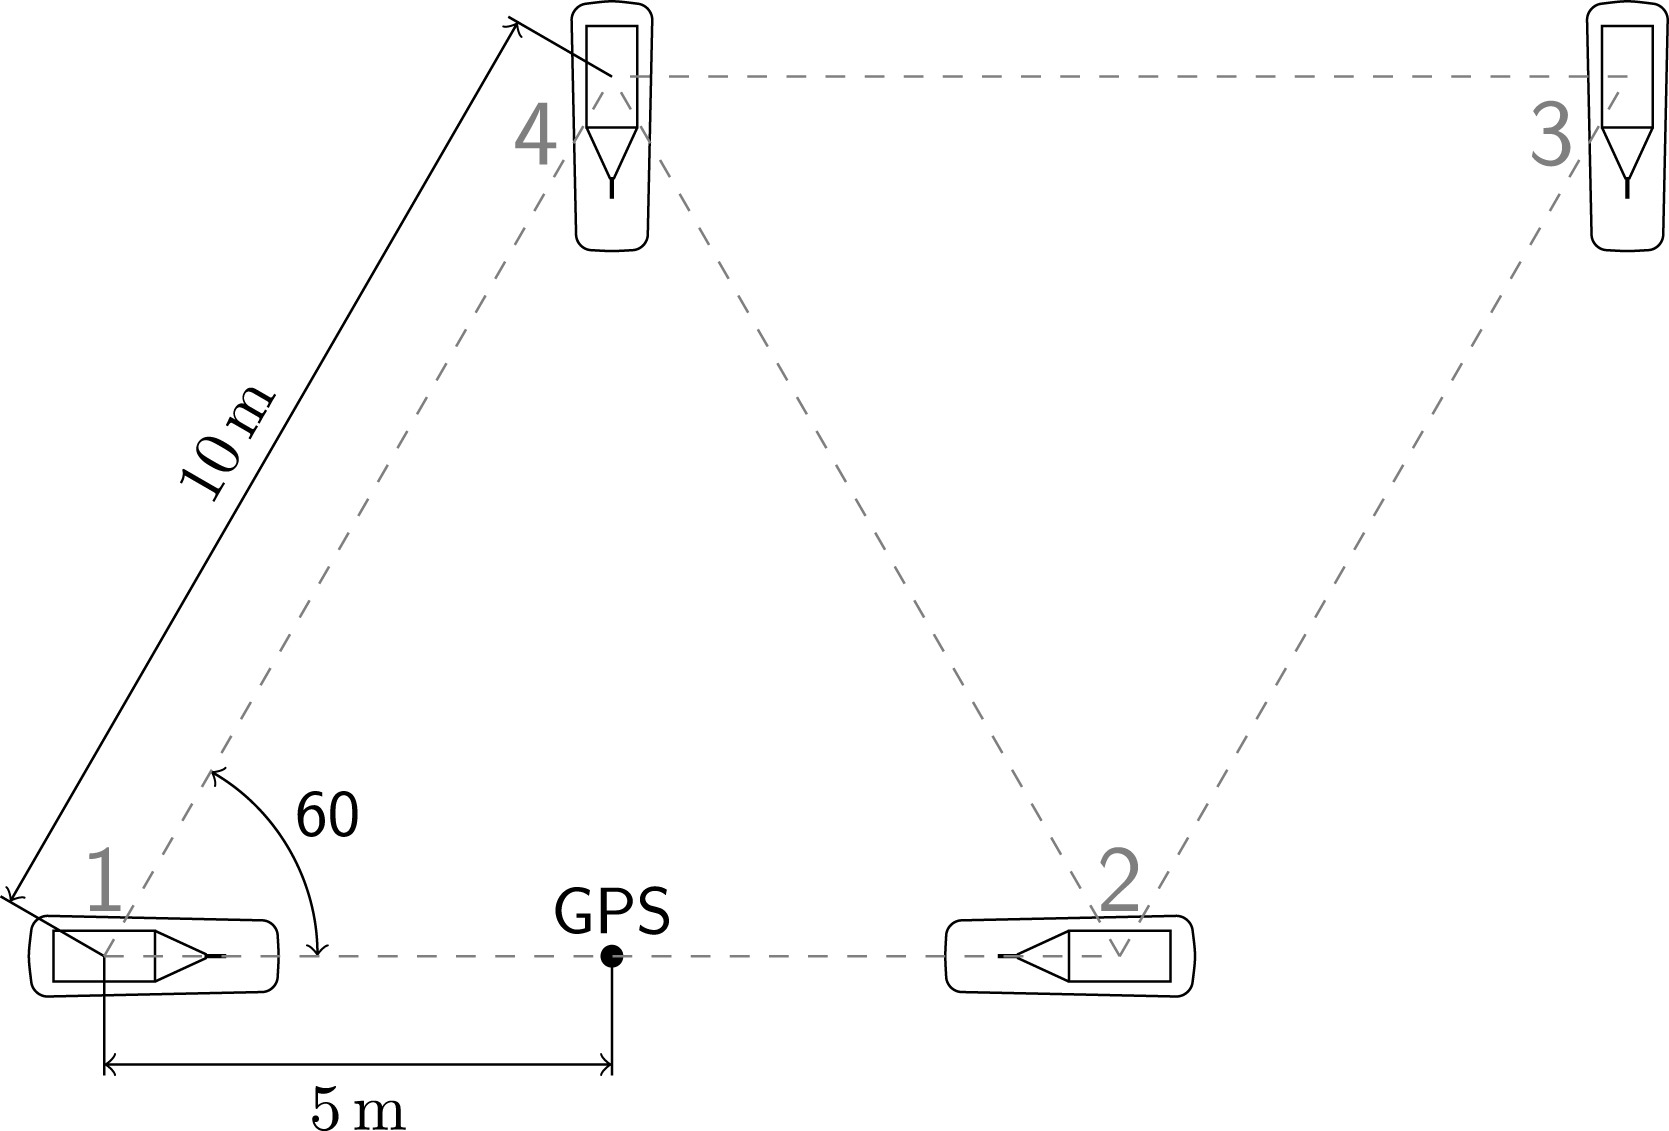
\includegraphics[width=0.5\columnwidth]{HS_4det-r.jpg}}
	\qquad
	\subfloat[Four-detector station configuration (diamond arrangement)]{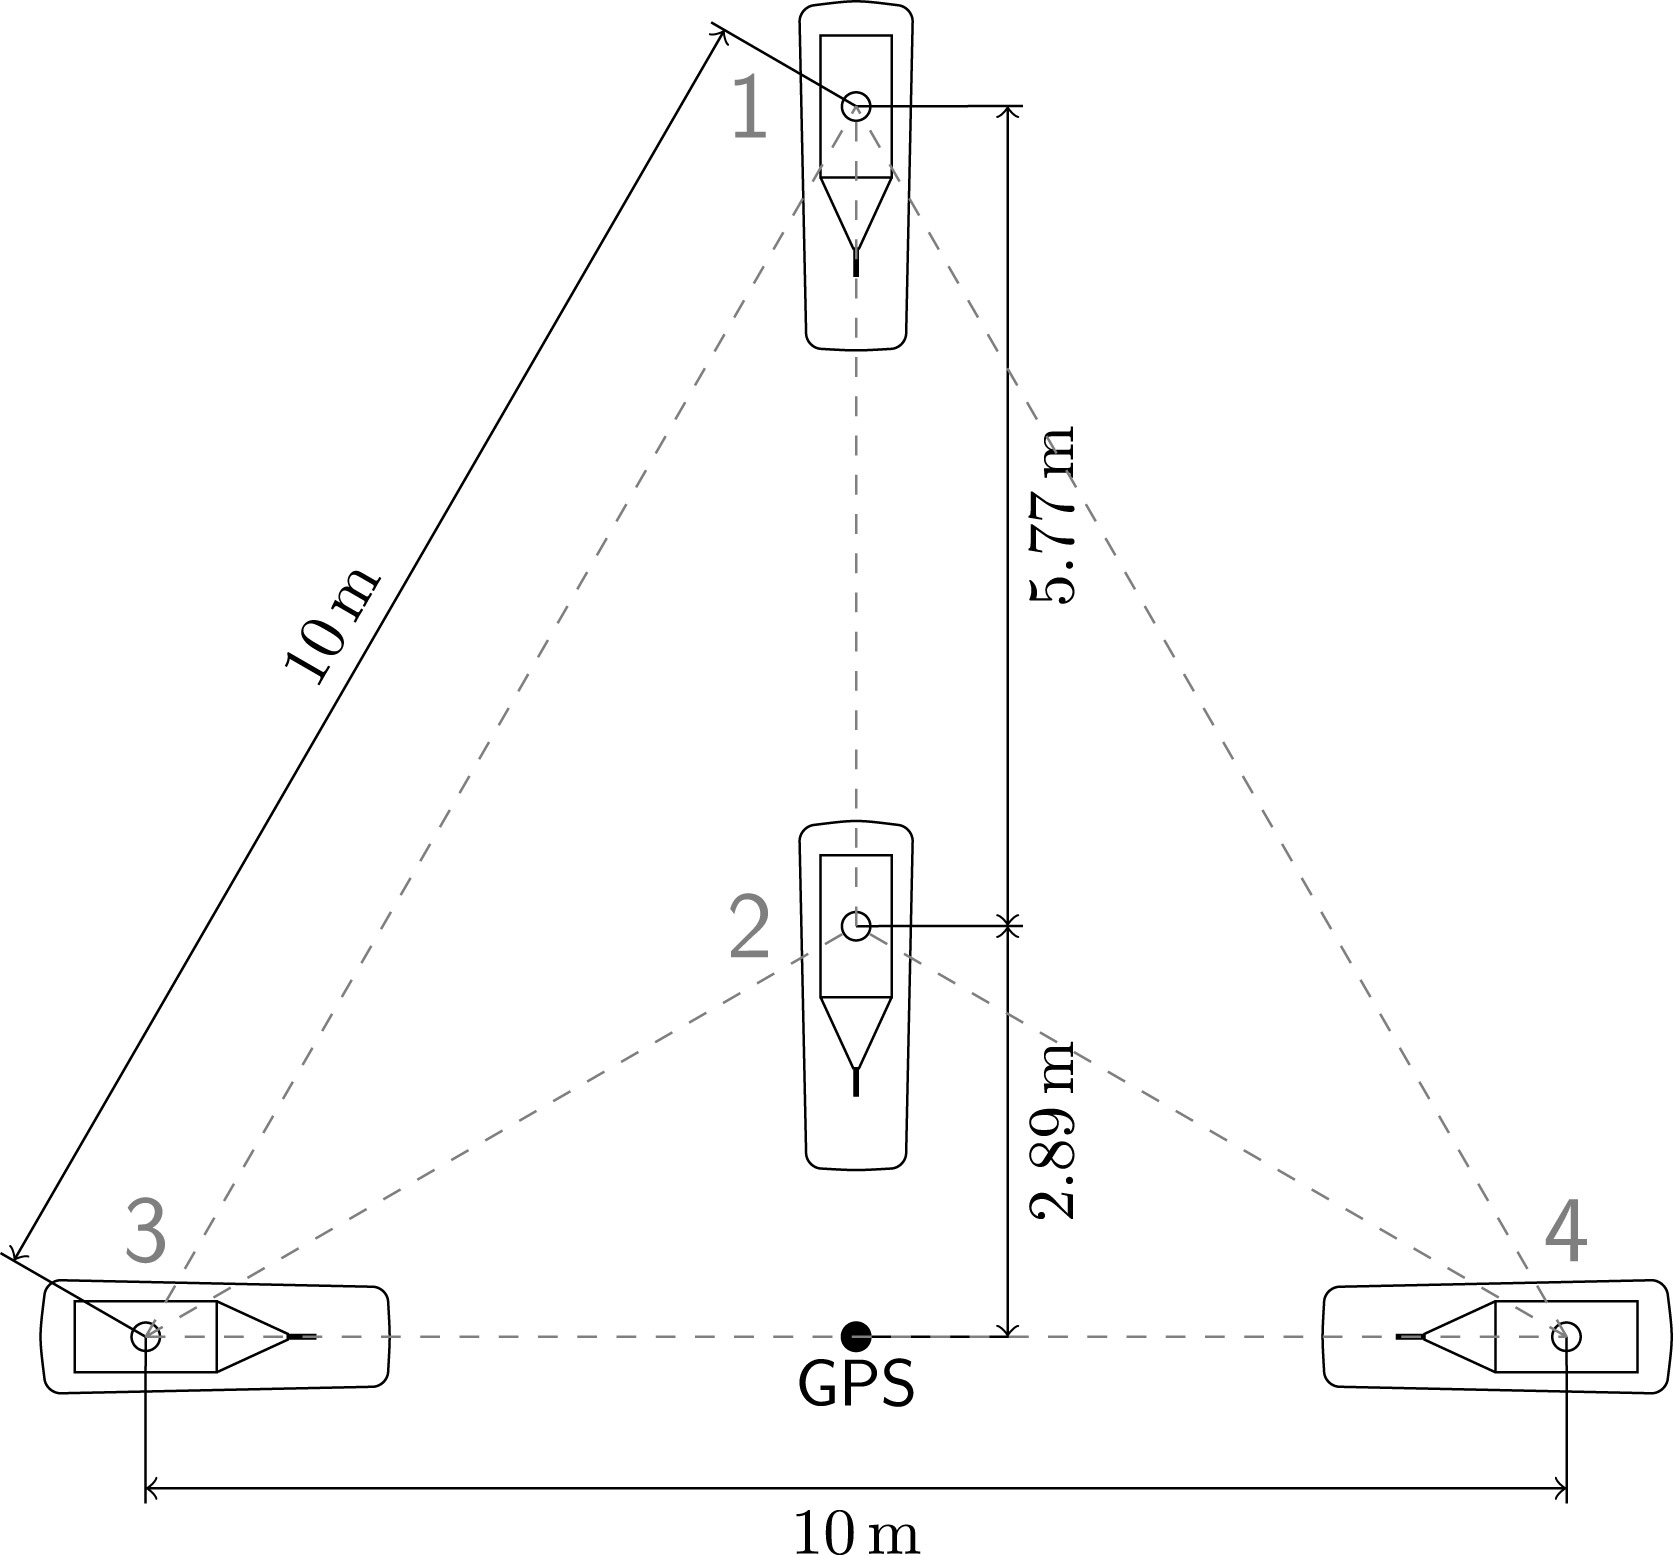
\includegraphics[width=0.5\columnwidth]{HS_4det-d.jpg}}
	\caption{Typical formations of two-detector and four-detector stations \citep{fokkema_hisparc_2012, van_dam_hisparc_2020}. In each, the black circle denotes a GPS antenna which is located in between the detectors to provide a precise timestamp for each signal.}
	\label{fig:HS_station_layouts}
\end{figure}


Furthermore some stations have the capability to measure the local atmospheric properties, such as temperature, pressure, relative humidity etc. Moreover, some stations also record the `singles' rates, i.e. the frequency at which an individual detector is triggered, independently of the other detectors in the station. The singles rates are important when investigating non-\gls{eas} events.

The scientific goals that can be achieved also vary between the two- and four-detector stations. When at least three detectors in a four-detector station observe particles of an \gls{eas}, the direction of the \gls{eas} (and thus the direction of the \gls{pcr}) can be acquired using triangulation calculations. When only two detectors in a station observe particles of an \gls{eas} it is only possible to reconstruct the arrival direction along the axis that connects the centres of those two detectors (thus it is not possible to reconstruct the direction of the \gls{pcr}).

The \glspl{pmt} of the detector in a station are connected to a \gls{hisparc} electronics box, which samples and digitises the signal at a rate of 400~MHz, and each \glspl{pmt} is connected to the electronics box using cables of a standard length of 30~m, to minimise any timing offsets between detectors \citep{fokkema_hisparc_2012, van_dam_hisparc_2020}. A schematic diagram showing the configuration of, and interfaces between, the \gls{hisparc} hardware is shown in Figure~\ref{fig:HS_hardware_config}. The electronics boxes are capable of controlling and reading two \glspl{pmt} (see Fig.~\ref{fig:HS_hardware_config}), therefore a four-detector station requires two electronics boxes: a primary and a secondary.


\begin{figure}[ht!]
	\centering
	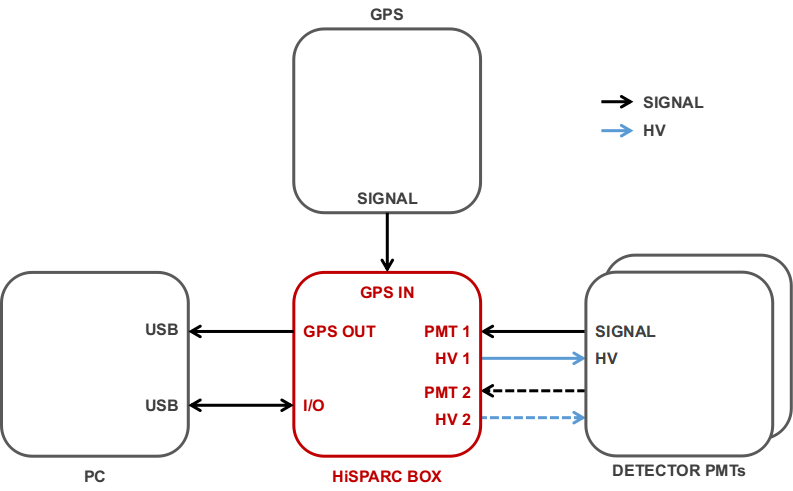
\includegraphics[width=\columnwidth]{HS_hardware_config.png}
	\caption{A schematic diagram showing the configuration and interfaces between the HiSPARC hardware for a two-detector station.}
	\label{fig:HS_hardware_config}
\end{figure}

Figure~\ref{fig:HS_hardware_config} shows all the hardware interfaces with the \gls{hisparc} electronics box, which communicates with the PC via USB. There are two connections for each \gls{pmt}, one for the control (i.e. \gls{hv}) and another for the signal. In addition, a \gls{gps} antenna is located in between the detectors in the station (shown in Fig.~\ref{fig:HS_station_layouts}). The \gls{hisparc} electronics box contains a \gls{gps} board, which provides an accurate timestamp for the data \citep{fokkema_hisparc_2012}.



%%%%%%%%%%%%%%%%%%%%%%%%%%%%%%%%%%%%%%%%%%%%%%%%%%%%%%%%%%%%%%%%%%%%%
\subsection{HiSPARC Data Acquisition}

\gls{hisparc} \gls{daq} software is used to control and read-out from the \gls{hisparc} electronics box. The \gls{daq} software was developed using LabVIEW, to be executed on a Windows PC \citep{van_dam_hisparc_2020}. Figure~\ref{fig:HiSPARC_trace} shows the typical output signal from one of the \glspl{pmt}, recorded by the \gls{daq} software. The depth of the trace is called the \textit{pulse height} and the area under the curve, the \textit{pulse integral}. The pulse integral is a measure of the number of scintillation photons that have arrived at the \gls{pmt}, exceeding the noise threshold ($-10$~mV) \citep{van_dam_hisparc_2020}. The \gls{hisparc} \gls{daq} software determines a signal baseline of the \gls{pmt} (i.e. the background signal without an incident muon), the pulse height, and pulse integral.

\begin{figure}[ht!]
	\centering
	\subfloat[Trigger pulse]{
		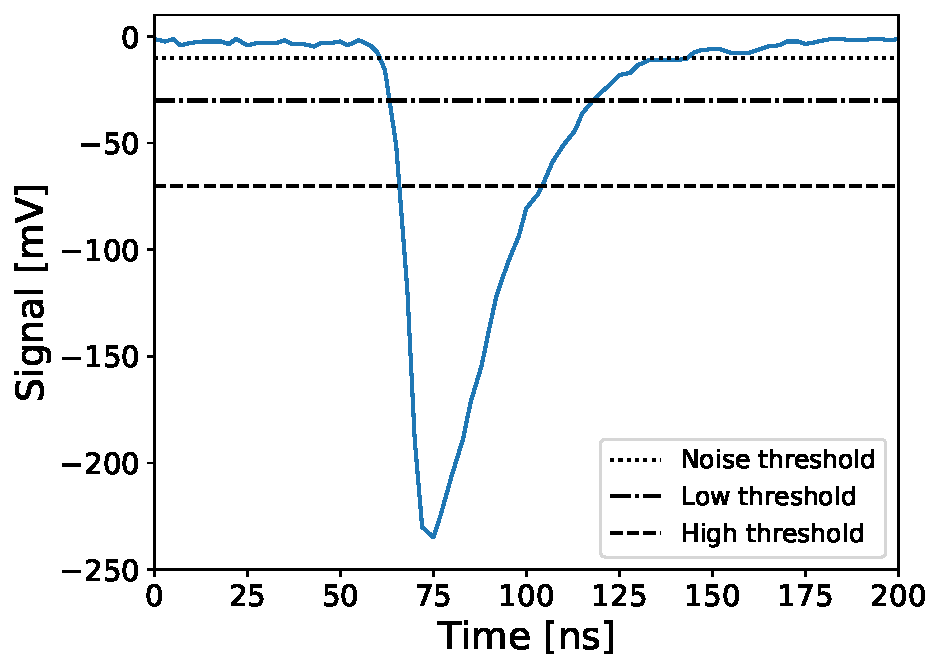
\includegraphics[width=0.48\columnwidth]{trace_plot.pdf}
		\label{fig:HiSPARC_trace}}
	%\qquad
	\subfloat[Pulse height spectrum]{
		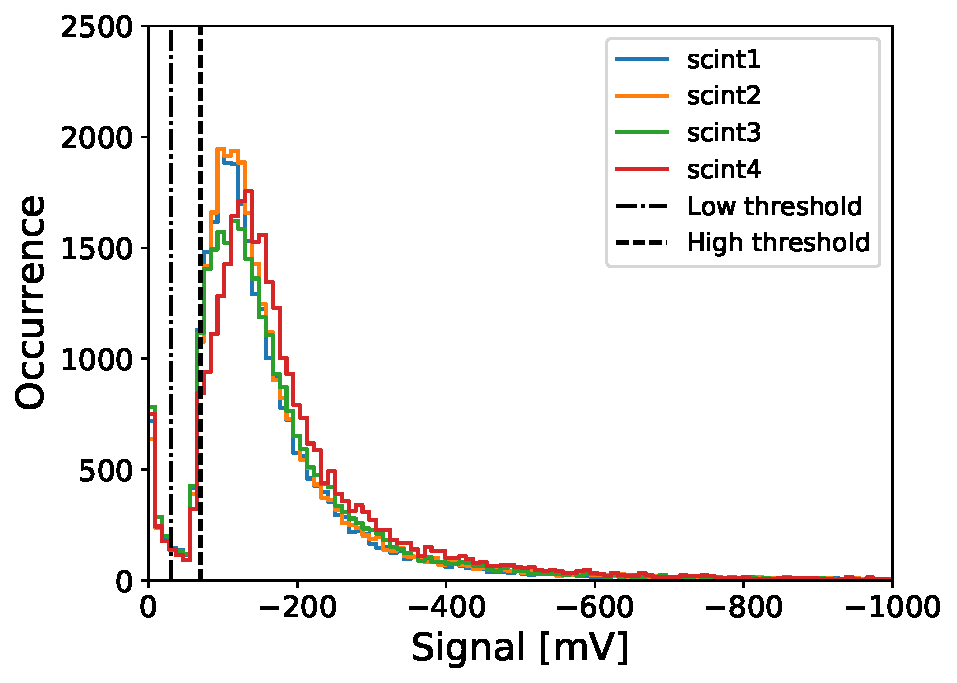
\includegraphics[width=0.48\columnwidth]{pulseheights.pdf}
		\label{fig:HiSPARC_pulseheight}}
	
	\caption{(a): An example PMT signal after digital conversion by the HiSPARC electronics box. The horizontal lines denote: the noise cut-off (dotted line), which is used for setting a limit when integrating the pulse height, to give the pulse integral; the low-voltage threshold (dash-dot); the high-voltage threshold (dashed). The role of the high- and low-voltage thresholds are described in the text below. (b) The pulse height distribution over the course of a single day from HiSPARC station 501. The vertical lines show the low-voltage threshold (dash-dot) and the high-voltage threshold (dashed).}
	\label{fig:pulses}
\end{figure}

The pulse height spectrum (see Fig.~\ref{fig:HiSPARC_pulseheight}) is a histogram of all the pulses recorded by a detector. It is composed of two main regions: the left side which falls off rather steeply, and the main, asymmetric part of the spectrum which features a peak and a long tail. The left side of the spectrum is understood to be from high-energy photons (gamma rays) produced in air showers \citep{fokkema_hisparc_2012}. These high-energy photons may undergo pair production when interacting with the scintillator which may produce ionising electron and positron pairs.

The main, asymmetric distribution, which features a peak and a tail, is from charged particles (i.e. muons and electrons) \citep{van_dam_hisparc_2020}. The mean energy loss of particles in a material is described by the Bethe-Bloch formula; however, this does not account for fluctuations in energy loss and a Landau distribution describes the fluctuations in energy loss of particles \citep{fokkema_hisparc_2012}. Due to the resolution of the \gls{hisparc} detectors the distribution in Figure~\ref{fig:HiSPARC_pulseheight} is best described by the convolution of the Landau distribution and a normal distribution which describes the resolution of the detector \citep{fokkema_hisparc_2012}. The peak of the distribution, the \gls{mpv}, is the most likely energy lost by a particle in the detector, i.e. the 3.51~MeV \citep{van_dam_hisparc_2020}. It has been shown that the location of the \gls{mpv} can vary due to the effects of atmospheric temperature \citep{bartels_hisparc_2012, van_dam_hisparc_2020}.

For each \gls{pmt}-channel, two discriminator thresholds can be defined: low- and high-voltage, as shown in Figure~\ref{fig:HiSPARC_pulseheight}, as vertical dash-dot and dashed lines, respectively.  The trigger thresholds are placed to reject the noise signals from the data, i.e. the left side of the pulse height spectrum. If a signal exceeds the high threshold, there is a high probability that the signal was generated by a particle in the detector. The `singles' data counts any time that the signal measured from a \gls{pmt} exceeds the low- or high-threshold.

The \gls{hisparc} experiment is configured in such a way as to ensure that each station across the \gls{hisparc} network measures a similar count rate of muons, in order to aid the direct comparison between the different stations in the network. When configuring the station, a trigger threshold must be applied for the \gls{pmt} signals. This is standardised across the \gls{hisparc} network and can be seen in relation to a detector trigger pulse in Figure~\ref{fig:HiSPARC_trace}. There are two thresholds, low: $-30$~mV, which represents $\sim0.2$ of a \gls{mip}; high: $-70$~mV, which represents $\sim0.5$ of a \gls{mip} \citep{fokkema_hisparc_2012, van_dam_hisparc_2020}. \citet{van_dam_hisparc_2020} states the thresholds were chosen to increase the sensitivity for observing gamma rays and low-energy electrons; the sensitivity is lower than for muons. However, as the detectors can measure gamma rays and electrons, it can be difficult to determine whether an individual detection was a muon, or another \gls{mip}, which is why the \gls{hisparc} network usually relies on detecting `events', from coincident muons.

To register an `event', the detectors must measure signals which exceed the low threshold, within a limited time window. The time-line of the data acquisition during an event is given in Figure~\ref{fig:HS_windows}.

\begin{figure}[ht!]
	\centering
	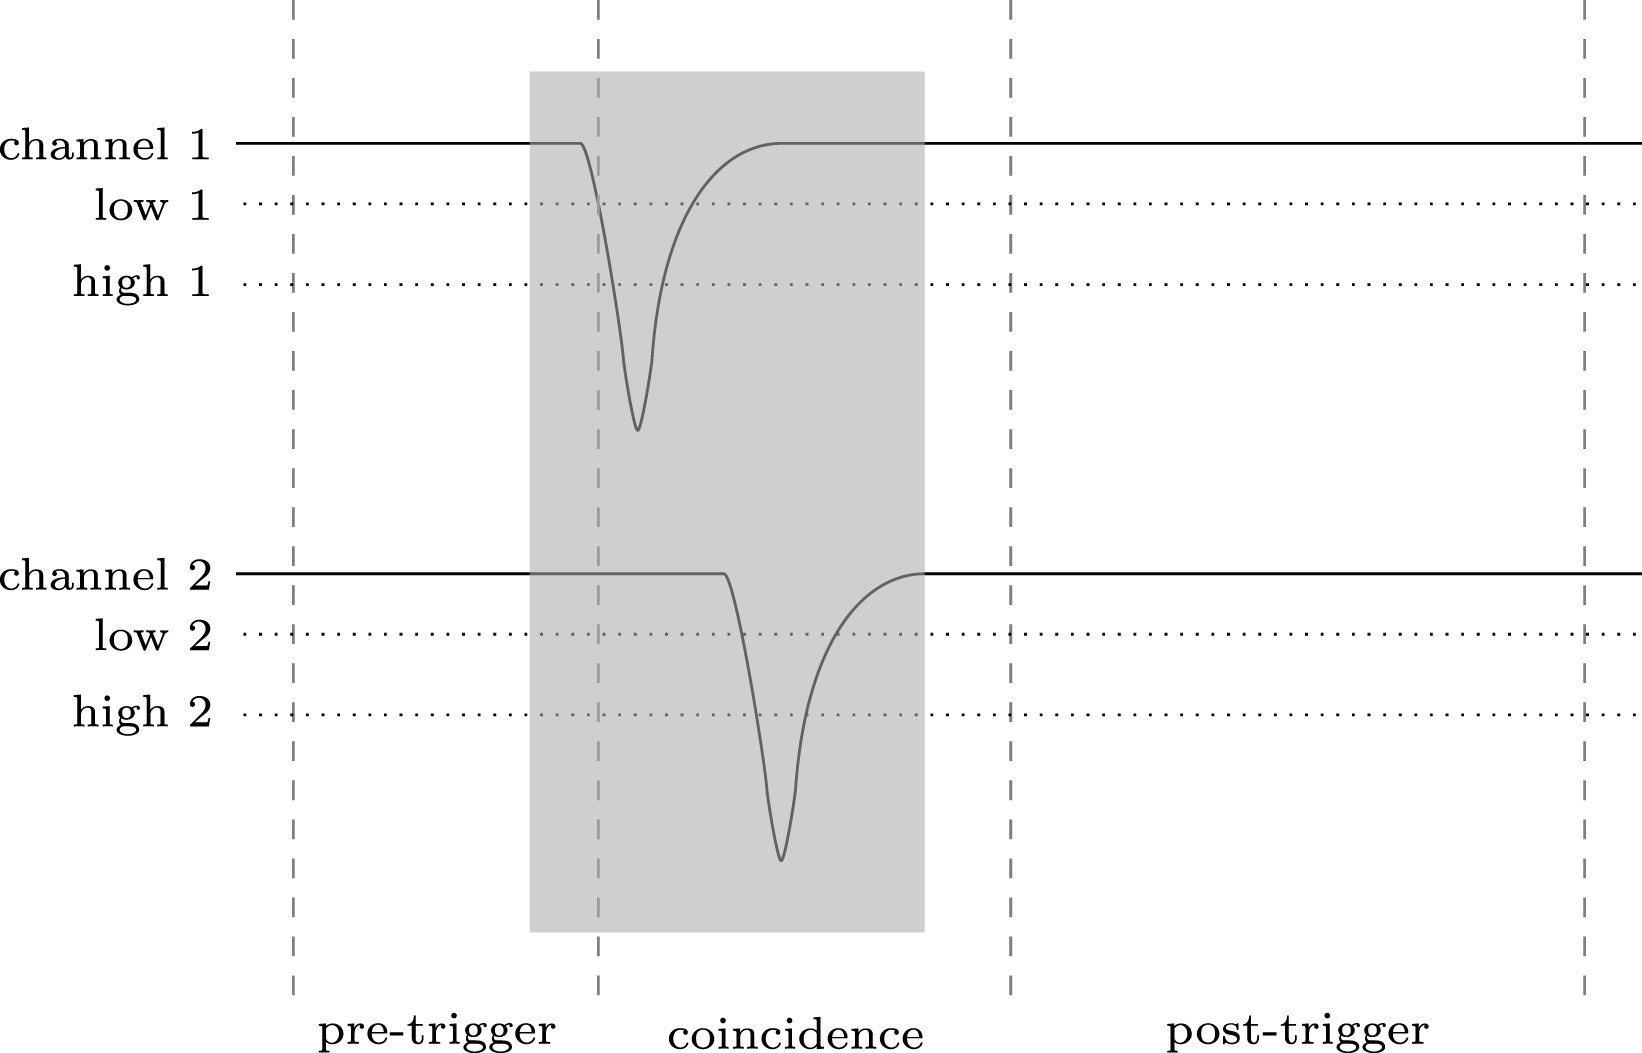
\includegraphics[width=0.9\columnwidth]{HS_pulses.jpg}
	\caption{Schematic data acquisition of an event \citep{fokkema_hisparc_2012}. The dashed vertical lines denote the epochs of the pre-trigger, coincidence, and post-trigger windows. The grey, shaded region shows the data reduction window and data outside this window are not stored. The dotted, horizontal lines denote the low- and high-voltage thresholds.}
	\label{fig:HS_windows}
\end{figure}

When channel~1 (i.e. \gls{pmt}~1) exceeds the low-threshold a coincidence window is opened. The length of the coincidence window is $\sim1.5~\upmu\mathrm{s}$. If, within this window, channel~2 (i.e. \gls{pmt}~2) also measures a signal that exceeds the low threshold, the trigger condition is met and an event is generated. When a trigger is issued, the output is stored in the buffer of the \gls{fpga} in the \gls{hisparc} electronics box \citep{fokkema_hisparc_2012}. The data acquisition software reads the data from the buffer and the full event data consist of: (i) data measured before the coincidence window was opened (the pre-trigger window, typical length $\sim1~\upmu\mathrm{s}$); (ii) data measured within the coincidence window; (iii) data measured after the trigger period (the post-trigger window, typical length $\sim3.5~\upmu\mathrm{s}$). Therefore, the event window lasts for $\sim6~\upmu\mathrm{s}$ in total, with the maximum length of an event window of $10~\upmu\mathrm{s}$ \citep{van_dam_hisparc_2020}. Finally, a data reduction algorithm is applied on the full event window which determines the part of the signal containing the muon pulses---compared to the baseline---and removes the rest, thus greatly reducing the size of the event data \citep{fokkema_hisparc_2012}.
%algorithm determines the part of the signal containing the PMT pulses and removes the res


The default trigger condition for detecting an air shower event between multiple \glspl{pmt} within a station differs for a two- and four-detector station. In a two-detector station, an event is recorded if the \gls{pmt} signals from both detectors exceed the low threshold within the coincidence time window ($1.5~\upmu\mathrm{s}$). In a four-detector station, the default trigger condition is either: (i) at least two detectors exceed the high threshold within the coincidence time window; (ii) at least three detectors exceed the low threshold within the coincidence time window. These are the default conditions, but there are other, user configurable ways of triggering the station. Under these nominal conditions, each \gls{hisparc} station triggers events at a rate of $\sim1$~Hz, i.e. substantially lower than the flux stated in Section~\ref{sec:air_shower}.


%Each detector in the network is set up such that the pulse height spectrum peaks at a \gls{mpv} of $\sim 150$~mV (see Figure~\ref{fig:pulses}), and such that the high threshold allows a mean count rate on the order 100 counts per second and the low threshold allows a mean count rate of the order 400 counts per second; these can by tuned by adjusting the \gls{pmt} voltage. It could be argued that in setting up the detectors in this way, there is an immediate bias in the data to reject lower energy \glspl{cr}.


Data recorded by the \gls{hisparc} stations are stored and are available on the \gls{hisparc} Public Database\footnote{\url{https://data.hisparc.nl/}}, where each station is listed, grouped by local nodes. For every station one can see its ID, name, and a coloured square and circle displaying its current data delivery and \gls{daq} status, respectively. Clicking on any station takes you to a dedicated page which displays its data on a user-selected day. Where data are available, it is possible to download: %The data are stored in {\verb HDF5 } format but are downloaded in {\verb .tsv } format.
%
\begin{itemize}
	\item{events rate data: where multiple detectors in a station are triggered to satisfy that station's trigger condition;}
	\item{singles rate data: the count rates of the individual detectors within a station;}
	\item{weather data: meteorological data, including pressure and temperature;}
	\item{coincidences data: the counts where different stations measure the same event (to within $1.36 \, \upmu$s); it is possible to determine if stations measured the same event by comparing the \gls{gps} timestamps of events.}
\end{itemize}

To support the \gls{hisparc} project, the \gls{sapphire} Python package \citep{fokkema_hisparc_2012,fokkema_sapphire_2012} was written. This Python package provide a framework to analyse the \gls{hisparc} data, but also an alternative way to acquire the data.



%To discriminate against single particle sources, \gls{hisparc} applies the ’coincidence method’. By using two (or four) detectors and selecting coincident PMT pulses (i.e. with a time difference smaller than 1.5 µs) the majority of random coincidences are rejected. If two or more PMT pulses exceed the threshold within the trigger window, the pulses are stored




\glsresetall 
{}
%%%%%%%%%%%%%%%%%%%%%%%%%%%%%%%%%%%%%%%%%%%%%%%%%%%%%%%%%%%%%%%%%%%%%%%%
%%%%%%%%%%%%%%%%%%%%%%%%%%%%%%%%%%%%%%%%%%%%%%%%%%%%%%%%%%%%%%%%%%%%%%%%
%%%%%%%%%%%%%%%%%%%%%%%%%%%%%%%%%%%%%%%%%%%%%%%%%%%%%%%%%%%%%%%%%%%%%%%%
\section{Thesis Structure}

In this thesis, a number of projects are presented which explore the themes of understanding the solar interior-atmosphere linkage and space weather applications. This is broken down into three major projects: a feasibility study on \gls{cr} space weather applications, an investigation into the effects of solar activity on \gls{cr} observations, and a study of the \gls{smmf}. The thesis is structured as follows:
%To clarify the structure of this thesis, the contents of each chapter and the main themes within are given in outline, before I present the work in each.

In Chapter~\ref{chap:HiSPARC} we perform a feasibility study to determine whether the \gls{hisparc} network is suitable for monitoring space weather events. This was achieved using historic data from the \gls{hisparc} network to search for the signature of space weather events. In addition we performed simulations of \glspl{as} to determine the expected variation in muon counts during space weather events. %At the time of writing, the work in this chapter had not been published in any journals.

Following the results of Chapter~\ref{chap:HiSPARC}, Chapter~\ref{chap:HiSPARC_14008} outlines the design and implementation on the University of Birmingham campus of an alternative \gls{hisparc} station, with a novel arrangement of detectors that removes thermally induced, diurnal variations in the data, and reduces the existing energy bias of observable \glspl{pcr} using the \gls{hisparc} network. In this chapter we discuss the set-up of the station, review the data and its noise properties, and finally also perform simulations using artificial data to investigate the capabilities of this new configuration. %At the time of writing, the work in this chapter had not been published in any journals.

In Chapter~\ref{chap:GCR_SSN_24} we studied long-term variations of \gls{gcr} intensity in relation to the \gls{ssn} during the most recent solar cycles. This study, which was published in the journal Solar Physics \citep{ross_behaviour_2019}, analysed the time lag between the \gls{gcr} intensity and the \gls{ssn}, and the hysteresis effect of the \gls{gcr} count rate against \gls{ssn} for Solar Cycles 20--24.

Chapter~\ref{chap:SMMF} presents a frequency-domain analysis of over 20~years of high-cadence \gls{bison} observations of the \gls{smmf}. We modelled the power spectrum of the \gls{bison} \gls{smmf} data to draw conclusions about the morphology of the \gls{smmf}, particularly focusing on the source of the rotationally modulated component in the signal. A significant portion of the work presented in this chapter was published in the journal Monthly Notices of the Royal Astronomical Society \citep{ross_lifetimes_2021}.

In Chapter~\ref{chap:rmode} we further investigated the \gls{bison} \gls{smmf} data. Here we examined the residual spectrum, after removing our best-fitting model, to search for evidence of a magnetic signature of global Rossby modes ($r$ modes). %At the time of writing, the work in this chapter had not been published in any journals.

We finish with concluding remarks in Chapter~\ref{chap:conc}.

All of the work and results presented in this thesis are my own and all the data analysis was performed by me. Input from others came in the form of advice and consultation, in addition to the supply of raw data.


%\chapter{Conclusions and Future Prospects}\label{chap:conc}

In this thesis, three studies have been presented, which investigated: using \gls{cr} detectors for space weather applications, the impact of solar activity of \glspl{gcr}, and solar interior-atmosphere linkages using observations the \gls{smmf}. %This work explores the interplay between the magnetic activity cycle and its effects as observed on the Earth.

In Chapter~\ref{chap:HiSPARC} we explored the properties and observations of the \gls{hisparc} experiment, to determine the feasibility of its use for monitoring space weather events. Using simulations of the interactions between \glspl{cr} and the Earth's magnetosphere, we were able to calculate the rigidity cut-off and \glspl{avd} of the \gls{hisparc} stations. We showed that the rigidity cut-off limits the observable \glspl{pcr} to those with energies on the order of and above $\sim 10^9$~eV. This highlighted that \gls{hisparc} stations would not observe the particles most susceptible to space weather events, i.e. those with energies $\sim 10^7-10^9$~eV.

We showed that we were unable to clearly detect signatures, in the raw \gls{hisparc} data, of the \glspl{fd} or \glspl{gle} that occurred over the lifetime of the \gls{hisparc} network. In addition, we showed that the effects of meteorological conditions caused variations in the data, which limited our ability to determine whether the events were observed in the raw data. A method to correct for the effects of atmospheric pressure and temperature was successfully demonstrated and applied to the \gls{hisparc} data. Following the correction of the atmospheric effects, the search for evidence of \glspl{gle} was repeated with the corrected \gls{hisparc} data. However, we concluded that we were also unable to clearly claim any observations of space weather events in the corrected \gls{hisparc} data.

\gls{as} simulations were employed to calculate the flux of muons at ground level. For low-energy \glspl{cr} ($\sim 10^9$~eV), we found the flux was small, producing very diffuse air showers of only a few muons, instead of the \glspl{eas} that \gls{hisparc} intends to observe. We showed the configuration of the \gls{hisparc} stations, which strongly relies on the triggering of multiple detectors within a station, biased observations to higher energy \glspl{pcr}, hence limiting the capabilities of using \gls{hisparc} network for space weather observations. This provided some explanation of why we were unable to detect the space weather events in the \gls{hisparc} data.

Furthermore, we ran simulations to predict the increase in the \gls{hisparc} count rate for some of the largest \glspl{gle} to-date. This showed, on average, we expect an increase in the muon count rate using the \gls{hisparc} detectors of $<1\%$, for a `typical' \gls{gle}. It was shown that only the most energetic events, with a lower occurrence rate, would induce an increase in the \gls{hisparc} counts by $\gtrsim5\%$. This provided further evidence to explain why we were unable to observe the \glspl{gle} and \glspl{fd} in the \gls{hisparc} data. Therefore we concluded that the \gls{hisparc} network is generally incompatible with monitoring the lower limits of space weather activity, and only suitable as a monitor of the rarer and more extreme events.


Leading on from these results, in Chapter~\ref{chap:HiSPARC_14008} we presented an alternative \gls{hisparc} station configuration, with a novel arrangement of the detectors, and investigated its performance for use monitoring space weather events. Firstly, we outlined the configuration and technical set-up of the station; secondly, we performed the relevant atmospheric corrections, where we showed that the new station provides an accurate measure of the temperature inside the roof boxes for station 14008, but also for the detectors of station 14001, which are located on the same building, on the University of Birmingham campus.

Using a Bayesian method to sample from the posterior distribution, we found the mean count rate of the new station configuration was $\sim80~\upmu/\mathrm{s}$, which was in good agreement with the predicted values from the air shower simulations in Chapter~\ref{chap:HiSPARC}. Furthermore, we determined the noise from spurious counts is of about $0.0043\pm0.0002~\upmu/\mathrm{s}$, which is negligible compared to the Poisson noise representing $\sim11~\%$ of the signal. Comparing the data to that collected by a nearby \gls{nm} station, Dourbes---in Belgium, we showed that there was a good visual agreement between the two data sets. This relationship should be continually monitored, as it will be instrumental in the verification of the new station configuration when/if a space weather event occurs in the next Solar Cycle.

Simulations of artificial data were performed to assess the likelihood of observing \glspl{gle} in the new station configuration. We demonstrated that with 10-s cadence observations we expect to be able to detect \glspl{gle} with a magnitude of $\gtrsim3~\%$. Furthermore, through averaging the data into 1- or 5-minute bins, we showed this improved the sensitivity, to observe \glspl{gle} with magnitudes $\gtrsim1.5~\%$. These values are in line with some of the predicted \gls{gle} magnitudes from Chapter~\ref{chap:HiSPARC}, providing compelling evidence to suggest that we should be capable of observing \glspl{gle} in this configuration.

We also simulated the performance of a network of detectors in this configuration and showed that we can improve the sensitivity to observe \glspl{gle} on the order of $\sim 1 \%$, through analysing the cross-correlation of nearby stations. However, we note that there is a strong dependence on decay time of the \glspl{gle}. We concluded that any upgrades to form a network of stations in this configuration should ideally use at least 5 stations, and 10 stations would be more beneficial.


\vspace{2em}


In Chapter~\ref{chap:GCR_SSN_24} we studied long-term variations of \gls{gcr} intensity in relation to the \gls{ssn} during the most recent solar cycles. We investigated the time lag between the \gls{gcr} intensity and the \gls{ssn}, and the hysteresis effect of the \gls{gcr} count rate against \gls{ssn} for Solar Cycles 20--24.

We showed that in cycle 24, the \gls{gcr} intensity lagged behind the \gls{ssn} by 2--4~months, which was slightly longer than the preceding even-numbered solar activity cycles (approx. 0--1~months). We showed the lag was not as large as the preceding odd-numbered cycles, and cycle 24 followed the trend of a short or near-zero lag for even-numbered cycles. We concluded that the cause of the extended lag in cycle 24 compared to previous even-numbered cycles was due to the deep, extended minimum between cycle 23 and 24, and the low maximum activity of cycle 24.

In addition, we showed the difference in the shapes of the hysteresis plots for odd-numbered and even-numbered cycles. The hysteresis plots were modelled using both a simple linear model and an ellipse model; the results showed that cycle 24 followed the same trend as preceding even-numbered cycles and was best represented by a straight line rather than an ellipse.

The time lag analysis was repeated using data from \gls{hisparc} station 501 (Nikhef). However, it was quantitatively concluded that there exists no correlation between the \gls{ssn} and the muon count rate measured by \gls{hisparc} station 501. The limiting factor to observe the effect was changes in set-up of the \gls{hisparc} station over time, which counteracted the expected variation due to solar activity.


\vspace{2em}


Chapter~\ref{chap:SMMF} presented a frequency-domain analysis of over 20~years of high-cadence \gls{bison} observations of the \gls{smmf}. If we convert a time series of the \gls{smmf} to the frequency-domain, a strong \gls{rm} signal appears as a series of peaks. This characteristic demonstrates that the source of the \gls{smmf} is long-lived, over several rotations. The power spectrum of the \gls{bison} \gls{smmf} data was modelled to draw conclusions about the morphology of the \gls{smmf}, particularly focusing on the source of the rotationally modulated component in the signal.

The duty cycle for the 40-second cadence observations was very low, hence the effect of the low fill on the power spectrum of the \gls{smmf} was investigated to inform how to best model the complete power spectrum. This highlighted that although there appeared to exist a red-noise-like, stochastic background component in the power spectrum, this was a feature originating from power aliasing, due to the low duty cycle of the observations. We had to be very cautious in our approach for modelling the power spectrum to ensure that Parseval's theorem was obeyed and that the effects of the window function were robustly accounted for.

Using a Bayesian approach, a model was fitted to the power spectrum. We found that the \gls{rm} component had a frequency of $0.4270\pm0.0018\,\upmu\mathrm{Hz}$. This frequency allowed us to infer the sidereal period of the \gls{rm} signal to be $25.23\pm0.11$~days which suggested cycle-averaged latitude of $\sim 12^{\circ}$, thus linking the source to active bands of latitude on the Sun. From the width of the \gls{rm} component peak, we were able to determine the lifetime of its source. We measured the lifetime to be $139.6\pm18.5$~days, which is in the region of $\sim20\pm3$~weeks.

The measured properties of the \gls{rm} component of the \gls{smmf} were consistent with \glspl{ar}. The literature provided compelling arguments to suggest that sunspots were not the origin of the \gls{smmf}, therefore we concluded that, more generally, \glspl{ar} and \glspl{mfc} are the source of the dominant, rotation signal in the \gls{smmf}, that are long-lived on the solar disc and exist in active latitudes. In addition, we demonstrated, numerically and analytically, that our ability to determine the linewidth and hence lifetime of the \gls{rm} modes was unaffected by \gls{ar} migration and differential rotation.


In Chapter~\ref{chap:rmode} we further investigated the \gls{bison} \gls{smmf} data to search for evidence of a magnetic signature of global Rossby modes ($r$ modes) in the residual power spectrum. A well-resolved peak was identified near the predicted $l=2=m$ $r$ mode frequency. Using a Bayesian modelling technique we found the peak was centred of frequency of $550\pm19$~nHz (i.e. $\sim9.2$~nHz from the predicted frequency, but within measured uncertainty). In addition we measured the width of the peak to be $5.2^{+4.9}_{-2.8}$~nHz, and amplitude to be $\sim 27.1^{+7.9}_{-5.9}$~mG. The properties of the measured peak were in agreement with observations of other sectoral $r$ modes and in-line with the predictions for the $l=2=m$ $r$ mode.

To understand the way the $r$ mode would manifest in the power spectrum, due to the variation in the B$_0$ angle we generated simulated data and acquired additional  hemispheric observations of the \gls{smmf} using full-disc magnetograms. Through the analysis of these data, we showed that we expected to see a prominent mode at the theoretical frequency, and not a split mode due to the effect of the B$_0$ variation. This further supported the hypothesis that the peak may have been the $l=2=m$ $r$ mode, assuming the magnetic $r$ mode signal had similar characteristics to the observed \gls{smmf} signal.

Finally, we investigated the power spectra of the \gls{smmf} observed with the \gls{wso} and \gls{sdo/hmi}, to verify if the peak was consistent across all observations. However, these observations showed no statistically significant peak in the location of the predicted $l=2=m$ $r$ mode frequency. It therefore ruled it highly unlikely that the candidate peak in the \gls{bison} spectrum was the $l=2=m$ $r$ mode. Because this peak was only observed in one of three data sets, and particularly not in the \gls{sdo/hmi} data which recent observations of sectoral Rossby waves in the Sun all used, we could not conclude that the candidate peak in the \gls{bison} spectrum was the $l=2=m$ $r$ mode. 


%%%%%%%%%%%%%%%%%%%%%%%%%%%%%%%%%%%%%%%%%%%%%%%%%%%%%%%%%%%%%%%%%%%%%
\subsection*{Future Prospects}

The first studies, presented in Chapter~\ref{chap:hisparc} and Chapter~\ref{chap:HiSPARC_14008}, of this thesis represented the beginning of exploring how the \gls{hisparc} network can be used to monitor space weather. The results from the first chapter showed that the \gls{hisparc} stations, in their original configurations, are not suitable for observing the effects of space weather; however, unfortunately, there have been few space weather events that have occurred over the lifetime of the \gls{hisparc} experiment and it is possible with more observations that we will observe the first space weather event with the existing \gls{hisparc} network. Continued monitoring of the data is imperative to check whether future space weather events are measured. This should be further supported by the observations from the \gls{gnmn} \citep{mishev_current_2020}, as they are proven to observe these events.

The air shower analysis to predict the variation in the muon count rate during space weather events was far from complete. We predicted the increase in muon intensity for only 6 of the 72 \glspl{gle} to-date. This was the limit of the analysis using the \gls{maire} tool used in this work. A more comprehensive analysis could be performed, using other sources of \gls{cr} spectra during space weather events, to predict the effect on the muon flux of the other \glspl{gle} and also \glspl{fd}.

The new station configuration shows promise to improve the space weather capabilities of the \gls{hisparc} network, and could be the beginning of a network-wide reconfiguration. The data collected by \gls{hisparc} station 14008 should be maintained until at least 2026, to ensure a complete study is performed up to the maximum of Solar Cycle 25 \citep{mcintosh_overlapping_2020, pesnell_lessons_2020}, when it is more probable that space weather events will occur. However, it would be of significant benefit to support this configuration for as long as possible, to compare the performance against the original \gls{hisparc} configuration for detecting space weather events.

The work presented in this chapter also investigated the effects of building a network of stations using this new configuration. It would be timely to create this network in the near-term, before cycle 25 maximum, such to benefit from the improved sensitivity at the time when more space weather events are expected.


\vspace{2em}


It is also of interest to revisit \citet{ross_behaviour_2019} (i.e. the work presented in Chapter~\ref{chap:GCR_SSN_24}) to: (i) confirm the conclusions are the same up to the end of cycle 24/start of cycle 25; (ii) investigate the properties of cycle 25; (iii) analyse consistent, good-quality data from the \gls{hisparc} network, in both the original configuration and station 14008 configuration, to observe the solar cycle modulation of \glspl{gcr}.


\vspace{2em}


Plans are in place to re-acquire observations of the \gls{smmf} using the Sutherland node of \gls{bison} and elsewhere. With more observations, the frequency resolution will improve, allowing for more accurate inferences on the \gls{smmf} morphology. Further to this, it would be interesting to investigate whether there exists a solar cycle dependence on the properties of the fitted peak. To do this, one could combine the data into separate maximum and minimum activity data sets, and re-run the analysis to determine if there are any differences. It would also be useful to do the same for rising and falling activity, to investigate the differences in the \gls{smmf} properties.

In addition, it would be beneficial to revisit some of the magnetogram thresholding techniques that are used in the literature, to pin-point which specific phenomena associated with \glspl{ar} cause the \gls{smmf}. We have shown that the source is manifested in long-lived \glspl{ar}, in active latitudes; probing this further would allow us to infer more information on morphology of the \gls{smmf}.

Finally, on the future prospects of the suspected Rossby mode in the \gls{bison} data. Again, as we collect more observations of the \gls{smmf} using \gls{bison}, the frequency resolution of the power spectrum improves. An obvious next step in this work is to collect more observations of the \gls{smmf} with \gls{bison}, to further investigate if this suspected mode remains resolved, or whether it diminishes into the noise. If still resolved, the investigation should be repeated, to determine the source of the signal.
%Blow this joint...

%HiSPARC
\chapter{HiSPARC as a Space Weather Detector}\label{chap:HiSPARC}

%%%%%%%%%%%%%%%%%%%%%%%%%%%%%%%%%%%%%%%%%%%%%%%%%%%%%%%%%%%%%%%%%%%%%
%%%%%%%%%%%%%%%%%%%%%%%%%%%%%%%%%%%%%%%%%%%%%%%%%%%%%%%%%%%%%%%%%%%%%
\section{Introduction}\label{sec:HS_intro}

... [on daily variations (DV)] Dr. Rolf Butikofer (in a reply from Danislav Sapundjiev, dasapund@meteo.be) said:

\textit{"The daily cosmic ray variation near Earth is caused by the anisotropy of the cosmic ray intensity in the interplanetary space. Cosmic ray particles follow the field lines of the interplanetary magnetic field when they travel towards the interior of the heliosphere. Because of the rotation of the Earth, the angle between the asymptotic cone of acceptance of various energies at the location of ground-based cosmic ray detectors (neutron monitors) and the direction of the interplanetary magnetic field varies with a time period of 24 hours. As a consequence cosmic ray detectors look in different directions in the course of a day and observe therefore a diurnal variation. The daily variations of neutron monitors is mainly seen by high latitude stations which have asymptotic directions at low energies (rigidities) near the equator."}


%%%%%%%%%%%%%%%%%%%%%%%%%%%%%%%%%%%%%%%%%%%%%%%%%%%%%%%%%%%%%%%%%%%%%
\subsection{HiSPARC Project}

%%%%%%%%%%%%%%%%%%%%%%%%%%%%%%%%%%%%%%%%%%%%%%%%%%%%%%%%%%%%%%%%%%%%%
\subsection{HiSPARC Detector}
 - design
 
 - scintillators
 
 - typical layouts (i.e. 2d or 4d)
 
 - trigger conditions


%%%%%%%%%%%%%%%%%%%%%%%%%%%%%%%%%%%%%%%%%%%%%%%%%%%%%%%%%%%%%%%%%%%%%
%%%%%%%%%%%%%%%%%%%%%%%%%%%%%%%%%%%%%%%%%%%%%%%%%%%%%%%%%%%%%%%%%%%%%
\section{Aims}\label{sec:HS_aims}
The HiSPARC project was set up with the detection philosophy of observing extended air showers (EAS), which are typically associated with PCRs with energy of $\sim10^{14}$~eV and above, that produce large footprints observable with many HiSPARC stations simultaneously. For PCRs with energy below $\sim10^{14}$~eV the air shower is small, with almost no observable footprint, and for PCRs with energy below $\sim10^{11}$~eV, there are typically less than one or two muons that reach the ground, making their observation difficult. 

The HiSPARC detectors are capable of observing any muons that reach them, therefore the project was motivated by the existing network of muon detectors which may have the capability of observing the cosmic rays associated with space weather events.

The principle aim of the project was to determine whether the existing HiSPARC network is capable of observing space weather events. This was initially achieved by investigating the data during periods of space weather activity to search for the associated signatures. In addition, simulations of air showers initiated by CRs were conducted to understand the expected muon flux at ground level.


%%%%%%%%%%%%%%%%%%%%%%%%%%%%%%%%%%%%%%%%%%%%%%%%%%%%%%%%%%%%%%%%%%%%%
%%%%%%%%%%%%%%%%%%%%%%%%%%%%%%%%%%%%%%%%%%%%%%%%%%%%%%%%%%%%%%%%%%%%%
\section{HiSPARC Properties}\label{sec:HS_properties}
 - Selected HS stations
 - Locations of stations
 - PLANETOCOSMICS simulations (explain)
 - Rigidities
 - Asymptotic viewing directions
 

To understand the PCR spectrum that the HiSPARC stations are capable of observing, PCR transport simulations were performed using the PLANETOCOSMICS software. PLANETOCOSMICS performs Geant4 Monte Carlo simulations of charged particle transport through Earth's magnetosphere based on St\o rmers transport equation for charged particles \citep{desorgher_planetocosmics_2006}. PLANETOCOSMICS simulates backward trajectories of charged particles from a given location (latitude, longitude, and altitude) out to the magnetopause for a set of PCR rigidites. 

For each trajectory there are two possible outcomes: (i) the particles trace out to the magnetopause where they escape Earth's magnetosphere, an allowed trajectory; (ii) the particles are sufficiently bent by the effect of the Earth's magnetosphere that they do not reach the magnetopause and cannot escape the Earth's magnetosphere, a forbidden trajectory \citep{desorgher_planetocosmics_2006}. The coordinates of the asymptotic direction at the magnetosphere are provided as an output to the simluations projected back down to the Earth's surface. In this work PLANETOCOSMICS was configured with the Tsyganenko-89 model for the external magnetospheric magnetic field and the IGRF internal field model.

For each rigidity simulated, whether it was an allowed or forbidden trajectory was stored, which was used to provide an insight into the rigidity spectrum for a given station. From the allowed trajectories the effective cut-off rigidity ($R_C$) for the stations was computed using equation~(\ref{eq:cut_off}), where $R_U$ is the upper rigidity (the last allowed trajectory before the first forbidden trajectory); $R_L$ is the lower rigidity (the last allowed trajectory before which all other trajectories with a lower rigidity are forbidden); $\Delta R$ is the rigidity step size in the simulation \citep{desorgher_planetocosmics_2006, herbst_influence_2013}.

\begin{equation}
\label{eq:cut_off}
R_C = R_U - \sum_{i = R_L}^{R_U} \Delta R_i
\end{equation}

The rigidity spectrum for each of the HiSPARC stations were investigated to determine $R_C$ for each station. The cut-off rigidity calculated for the six HiSPARC stations for a vertical incidence upon the atmosphere (i.e. $0^\circ$ zenith angle) are shown in Table~\ref{tab:HS_stns} which show that there is little variation in $R_C$ between the HiSPARC stations and that they observe protons with rigidities in excess of $\sim 3$ GV. This analysis was initially carried out for the vertical direction (i.e. azimuth = $0^\circ$, zenith = $0^\circ$); however further trajectories were simulated for different azimuth and zenith angles to determine the dependence of the rigidity spectrum on the detector acceptance angle. The analysis for the azimuthal dependence was carried out at a zenith angle of $20^\circ$ as this is around the most probably angle for HiSPARC events, and the analysis of the zenith dependence was carried out at an azimuth angle of $0^\circ$.


\begin{table}
	\begin{center}
		\caption{Properties of some of the HiSPARC stations: geographic longitude ($\lambda$), geographic latitude ($\phi$), altitude ($h$), and the geomagnetic vertical cut-off rigidity ($R_C$) calculated from the PLANETOCOSMICS simulations.}
		\label{tab:HS_stns}
		\begin{tabular}{l c c c c c}
			\hline
			& $R_C$  & $\lambda$ & $\phi$  & $h$  & No. Detectors\\
			Station Name/ID & [GV] & [deg] & [deg] & [m]  & \\
			\hline
			Nikhef/501 & 3.19 & 4.95 E & 52.36 N & 56.18 & 4 \\
			College Hageveld/203 & 3.18 & 4.63 E  & 52.35 N & 53.71  & 2 \\
			Leiden/3001 & 3.23 & 4.45 E & 52.17 N & 54.08 & 2 \\
			Eindhoven/8001  & 3.44 & 5.49 E & 51.45 N & 70.12 & 2 \\
			Birmingham University/14001  & 3.06 & 1.93 W & 52.45 N & 204.14 & 4  \\
			%20003 & 2.30 & 10.20 E & 56.17 N & 84.38 & 2 \\
			\hline
		\end{tabular}
	\end{center}
\end{table}

\begin{figure}[h]
	\centering
	\subfloat[Azimuth variation (fixed zenith = $20^\circ$)]{
		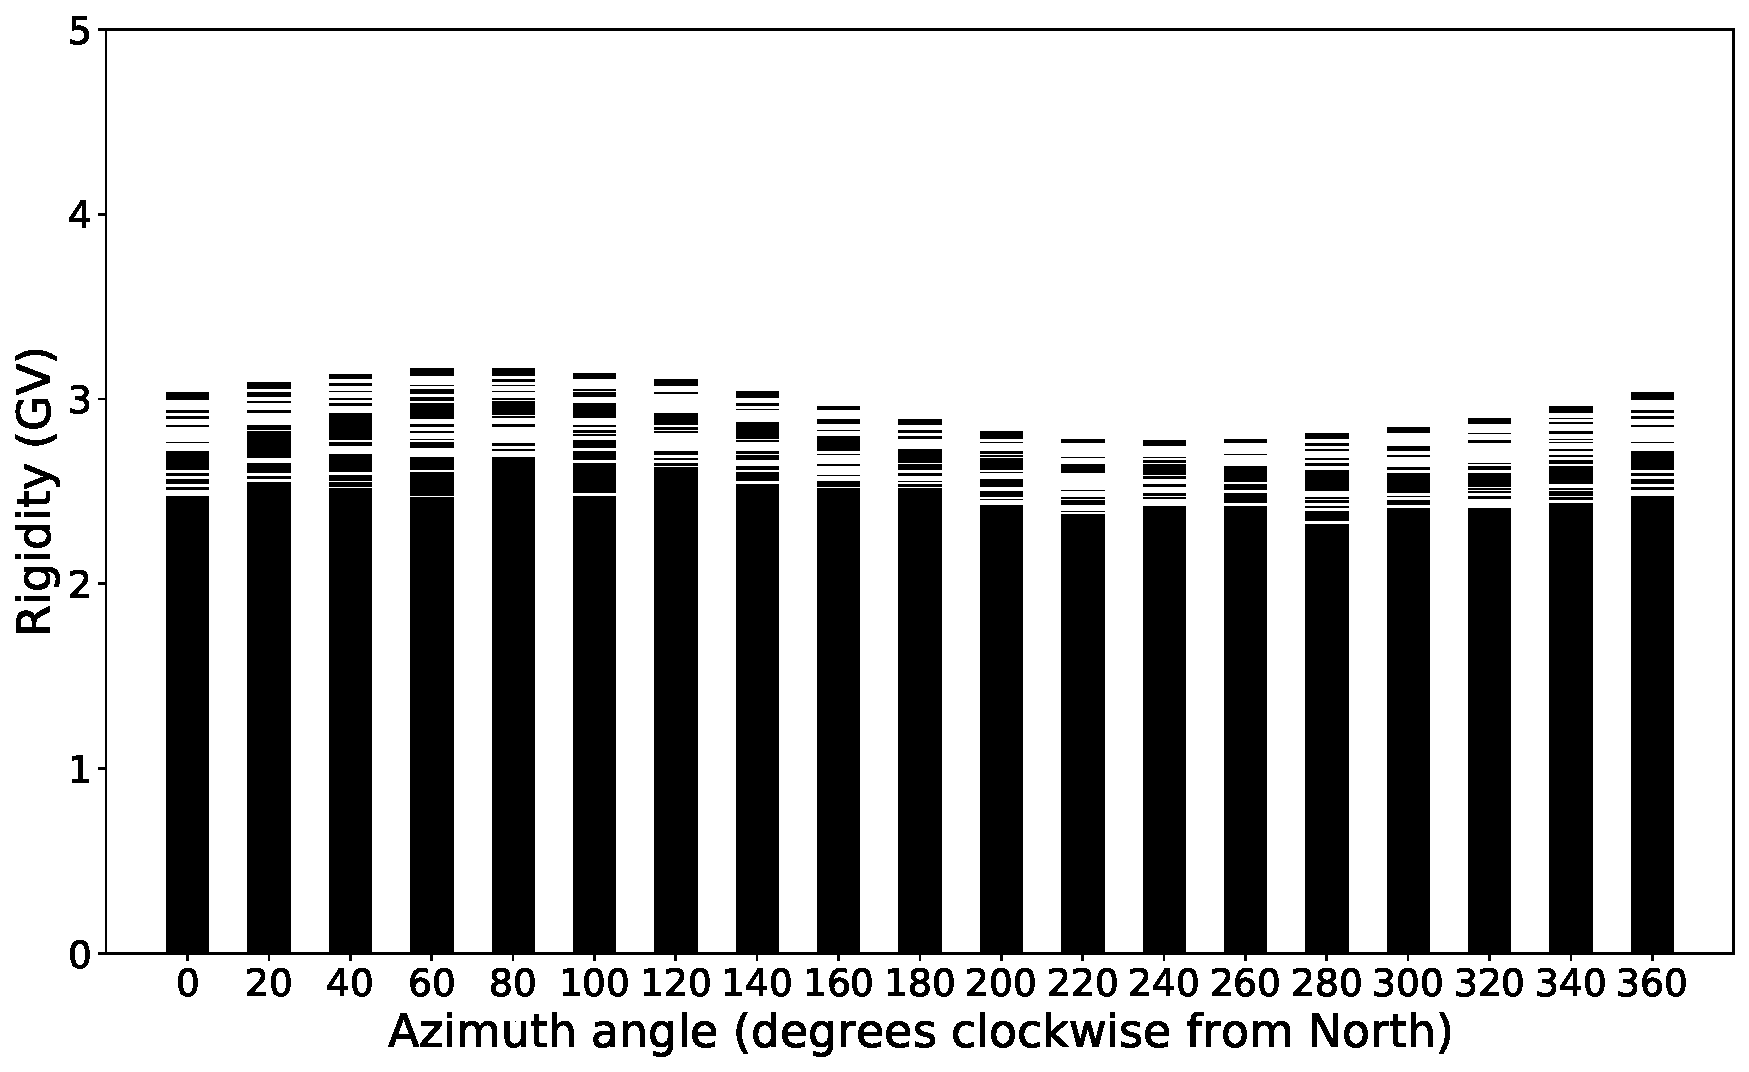
\includegraphics[width=0.48\columnwidth]{azm.pdf}
		\label{fig:azm1}}
	%\qquad
	\subfloat[Zenith variation (fixed azimuth = $0^\circ$)]{
		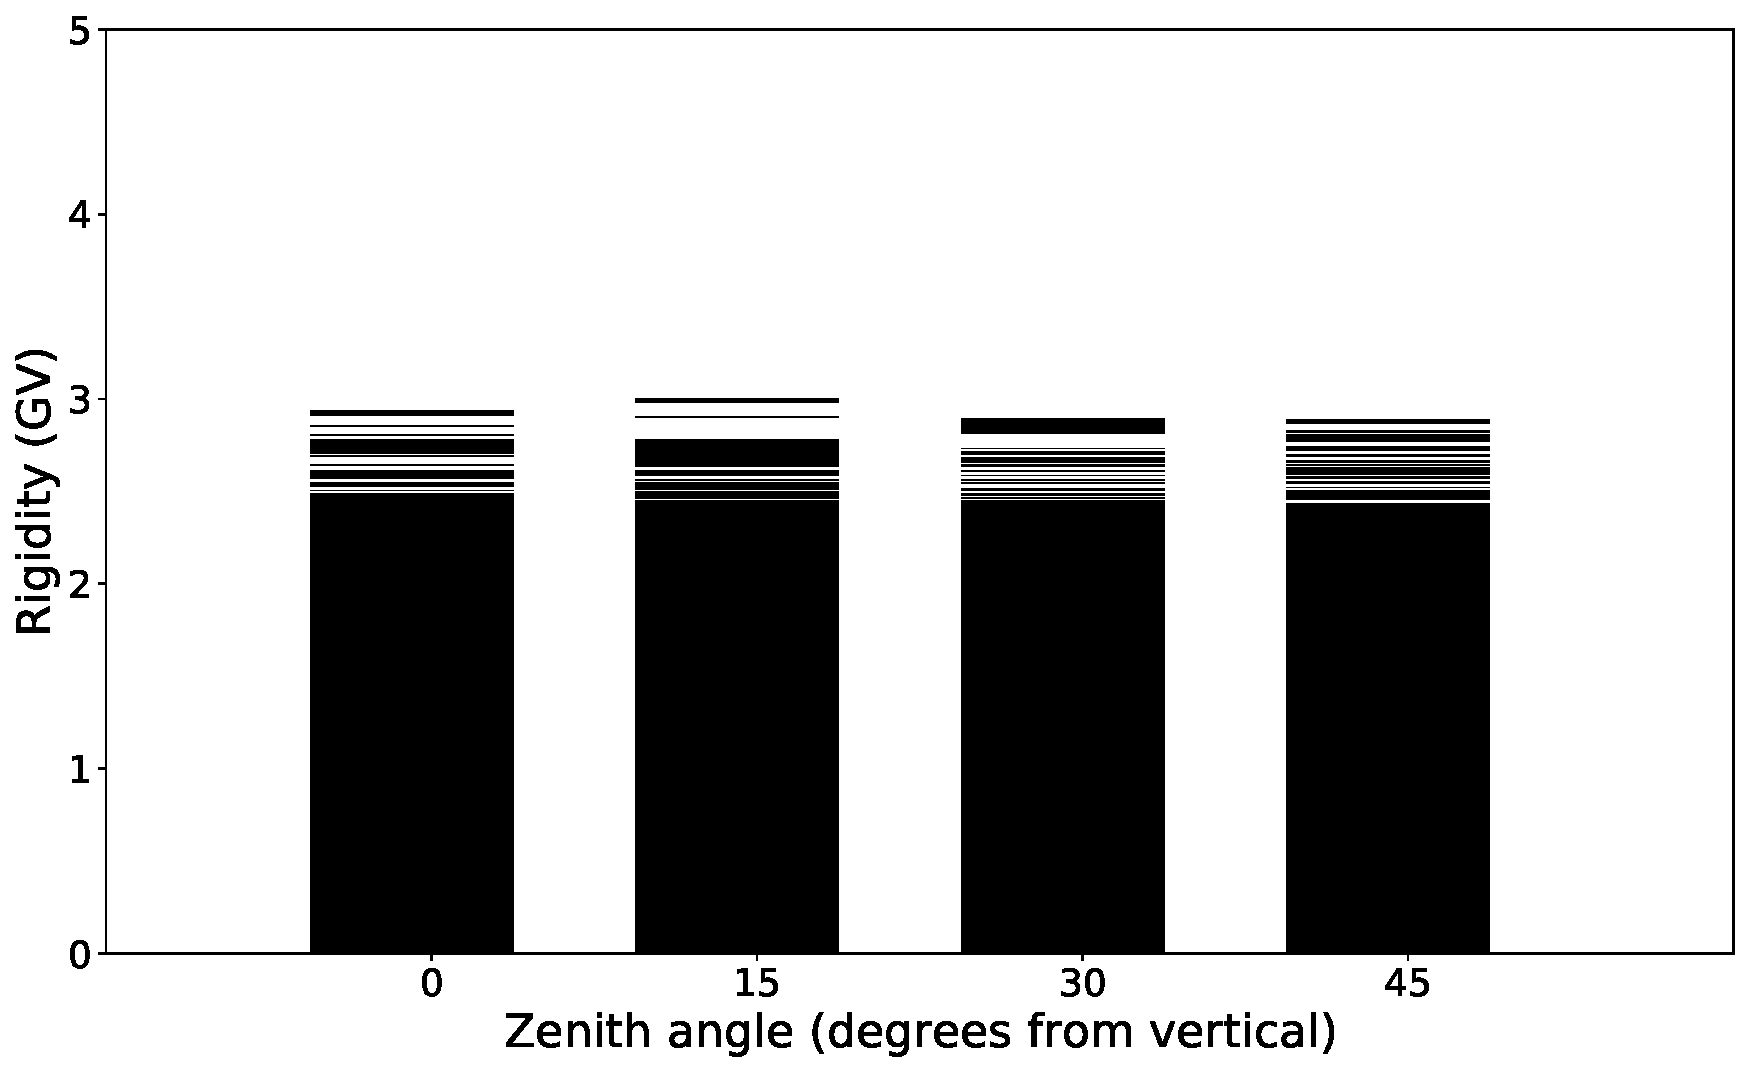
\includegraphics[width=0.48\columnwidth]{zen.pdf}
		\label{fig:zen1}}
	
	\caption{Azimuthal and zenith angle variations in the allowed and forbidden rigidity trajectories for HiSPARC station 501.}
	\label{fig:R_C2}
\end{figure}

The small variation between HiSPARC stations is due to their close proximity in geographic latitude and longitude. The values of $R_C$ calculated for the HiSPARC stations suggest that they should be able to observe higher energy SCRs, but may not be as susceptible as the higher latitude NMs where the effects of GLEs are highly observable.

As a results of the PLANETOCOSMICS simulations it is possible to understand the trajectories of particles that enter the Earth's magnetosphere prior to arrival at the muon detector.

Figre~\ref{fig:HS_AVD}...

\begin{figure}[ht]
	\centering
	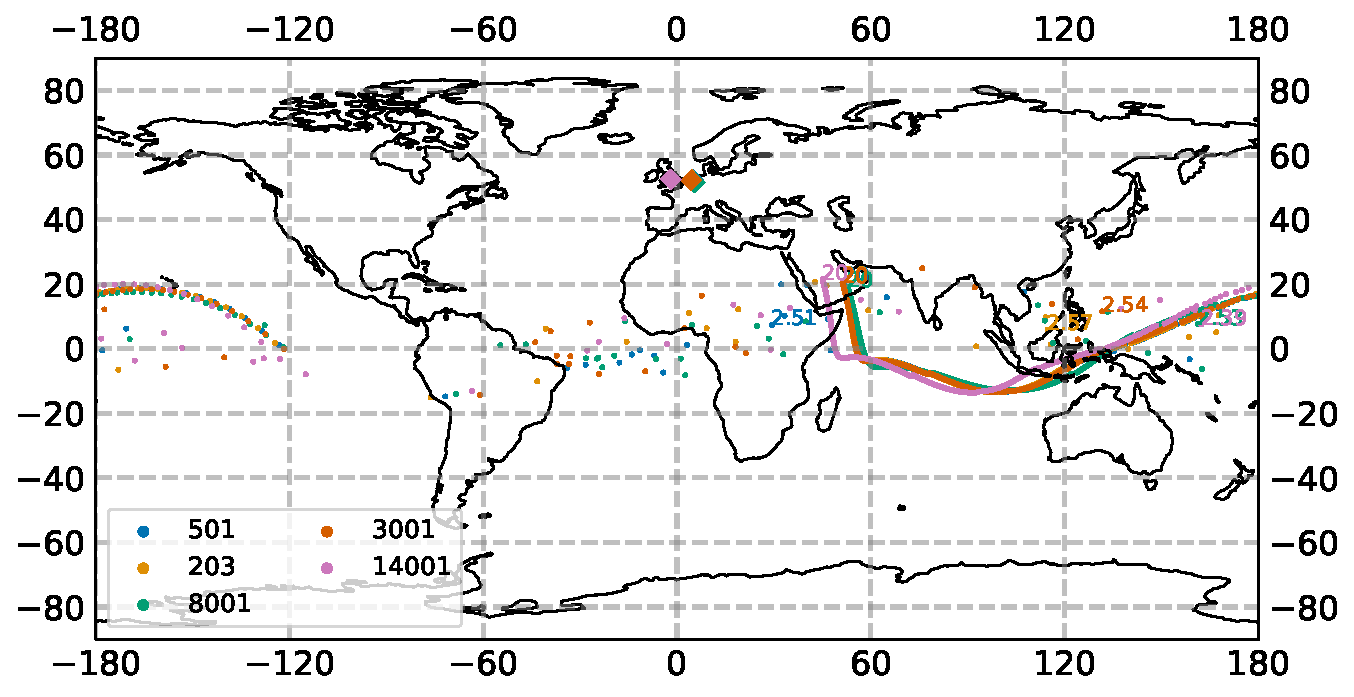
\includegraphics[scale=0.6]{HS_AVDs.pdf}
	\caption{The vertical asymptotic viewing directions of 5 HiSPARC stations. The rigidity range of the simulations were from $1.0$~GV $<$ R $<20.0$~GV, and the results are plotted in geographic coordinates on January 20th 2005. The diamonds correspond to the HS ground location and the circles correspond to the AVD for a specific rigidity value.}
	\label{fig:HS_AVD}
\end{figure}


 

%%%%%%%%%%%%%%%%%%%%%%%%%%%%%%%%%%%%%%%%%%%%%%%%%%%%%%%%%%%%%%%%%%%%%
%%%%%%%%%%%%%%%%%%%%%%%%%%%%%%%%%%%%%%%%%%%%%%%%%%%%%%%%%%%%%%%%%%%%%
\section{HiSPARC Observations}\label{sec:HS_obs}


[discuss preliminary observation of space weather FDs and GLEs for the events and singles data...]

[end with discussion on unknown PCRs observable and the effect of atmospheric weather conditions that need to be accounted for]

The effects of space weather on CRs has been outlined in [REF intro]. It was highlighted during communication with the UK Met Office that observations of GLEs are of more interest and importance to space weather forecasts and nowcasts. FDs are of lower interest and importance, however they were still searched for within the HiSPARC data. The events that were looked for within the HiSPARC data are outlined in Table~\ref{tab:space_weather_events}.

\begin{table}
	\begin{center}
		\caption{Space weather events investigated within the HiSPARC data. The percentage change column provides a reference of how much the CR counts observed by the NM station at Oulu (R$_c$=0.81~GV) increased of decreased by, due to the space weather event.}
		\label{tab:space_weather_events}
		\begin{tabular}{c c c | c c}
		\hline
		{\bf GLE Onset} & {\bf GLE} & {\bf \% Change (Oulu)} & {\bf FD Onset} & {\bf \% Change (Oulu)}\\
		\hline
		{13/12/2006} & {70} & {$\sim 100\%$} & {08/03/2012} & {$\sim 5\%$}  \\
		{17/05/2012} & {71} & {$\sim 15\%$} & {14/07/2012} & {$\sim 3\%$} \\
		{10/09/2017} & {72} & {$\sim 5\%$} & {21/12/2014} & {$\sim 5\%$} \\
		{} & {} & {} & {06/09/2017} & {$\sim 2\%$} \\
		{} & {} & {} & {07/09/2017} & {$\sim 8\%$} \\
		\hline
		\end{tabular}
	\end{center}
\end{table}



%%%%%%%%%%%%%%%%%%%%%%%%%%%%%%%%%%%%%%%%%%%%%%%%%%%%%%%%%%%%%%%%%%%%%
\subsection{HiSPARC Observations of Ground Level Enhancements}

Initial searches for evidence of GLEs within the HiSPARC data were conducted for GLE 70, 71, and 72, as they arethe only GLEs that span the operational epoch of the HiSPARC network.

Figure~\ref{fig:GLE_70}...

\begin{figure}[h]
	\centering
	\subfloat[HS 501 (Nikhef)]{
		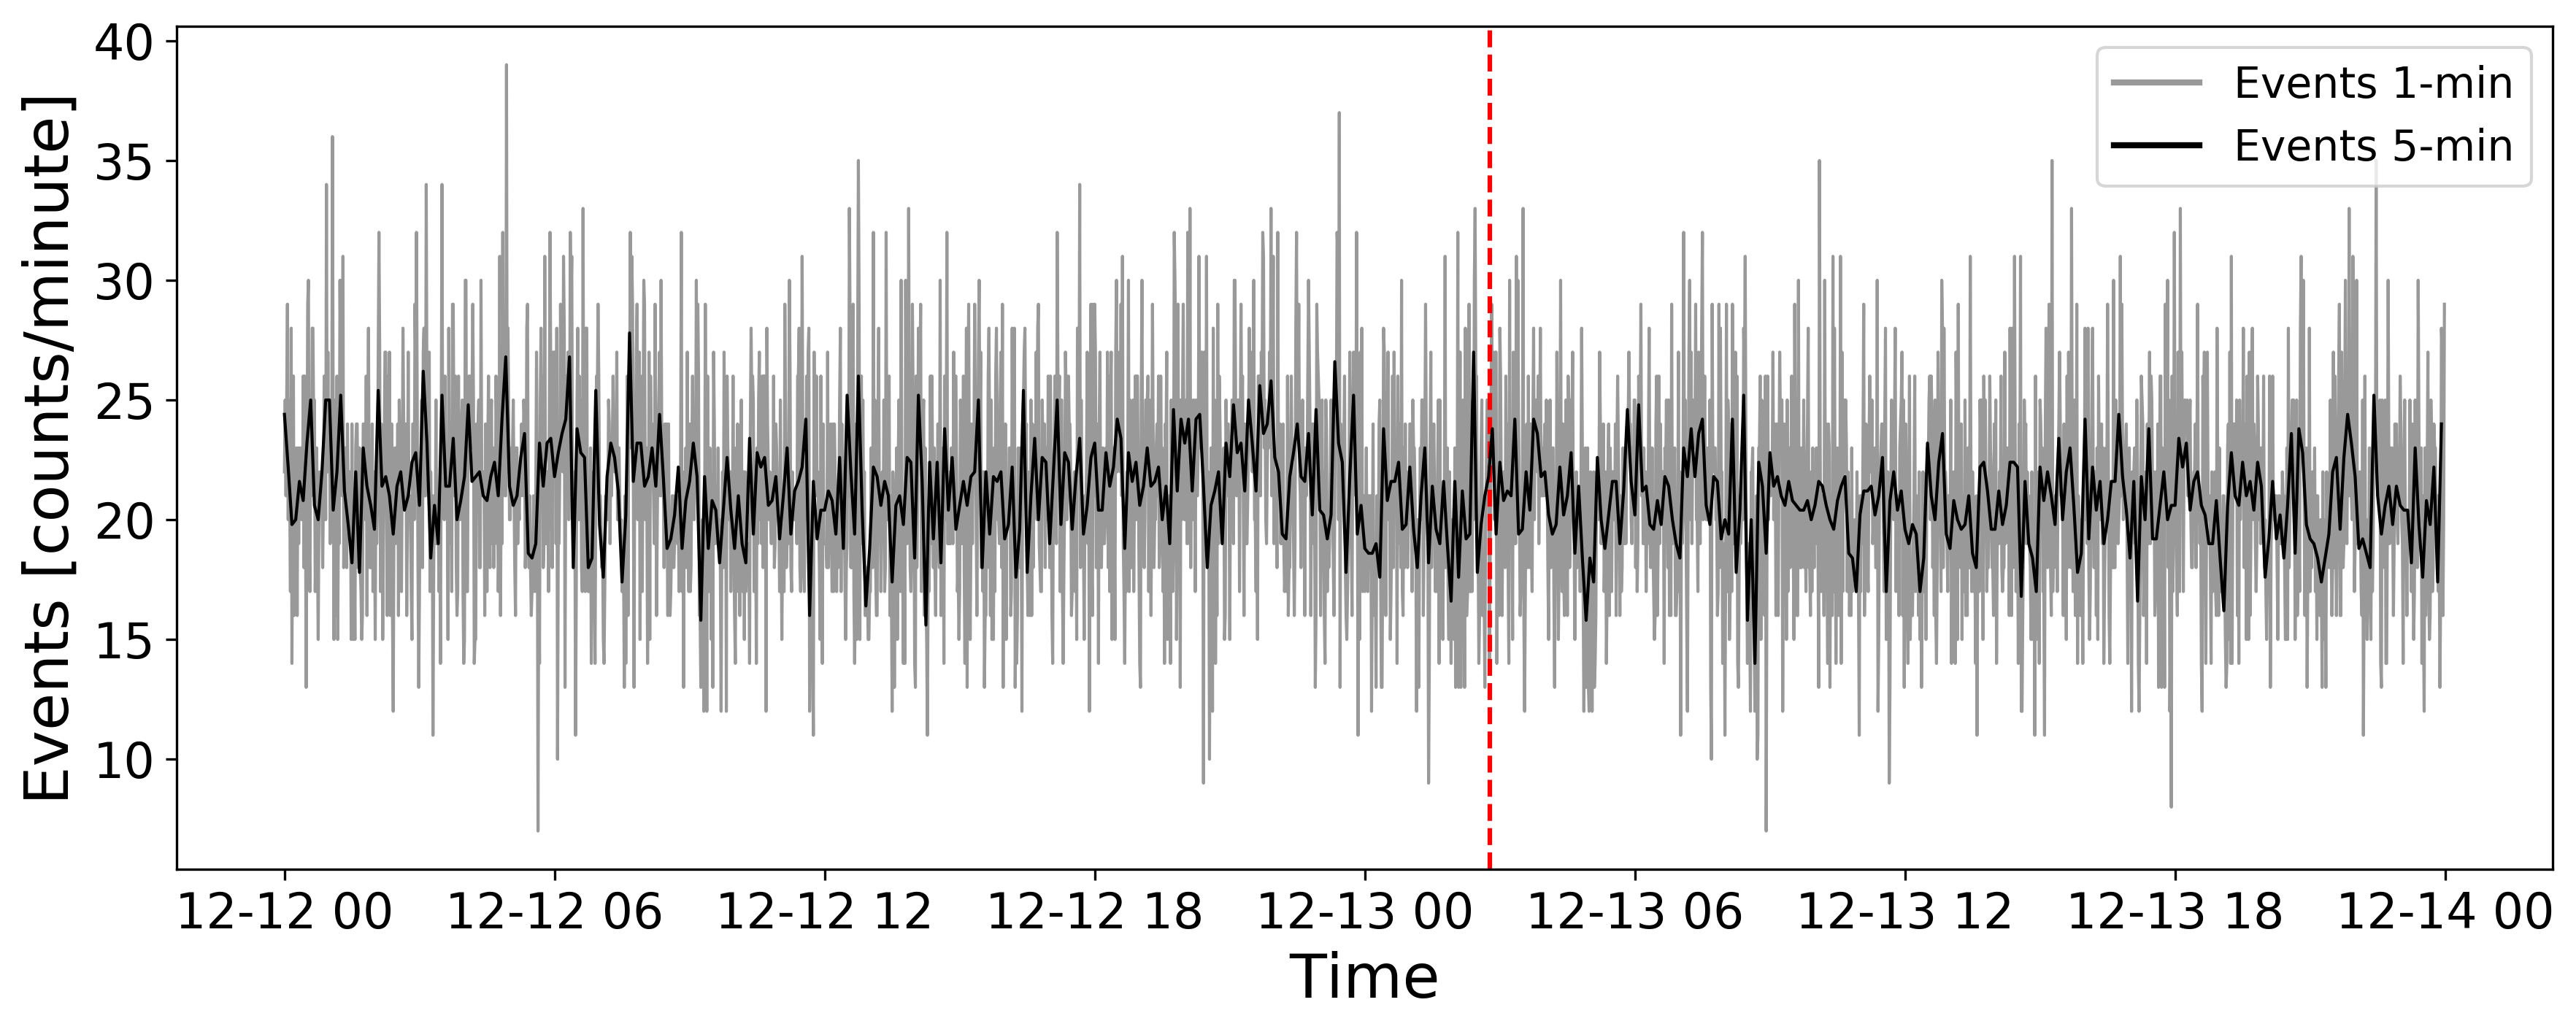
\includegraphics[width=0.48\columnwidth]{GLE70_501.png}
		\label{fig:GLE70_501}}
	%\qquad
	\subfloat[HS 3001 (Universiteit Leiden)]{
		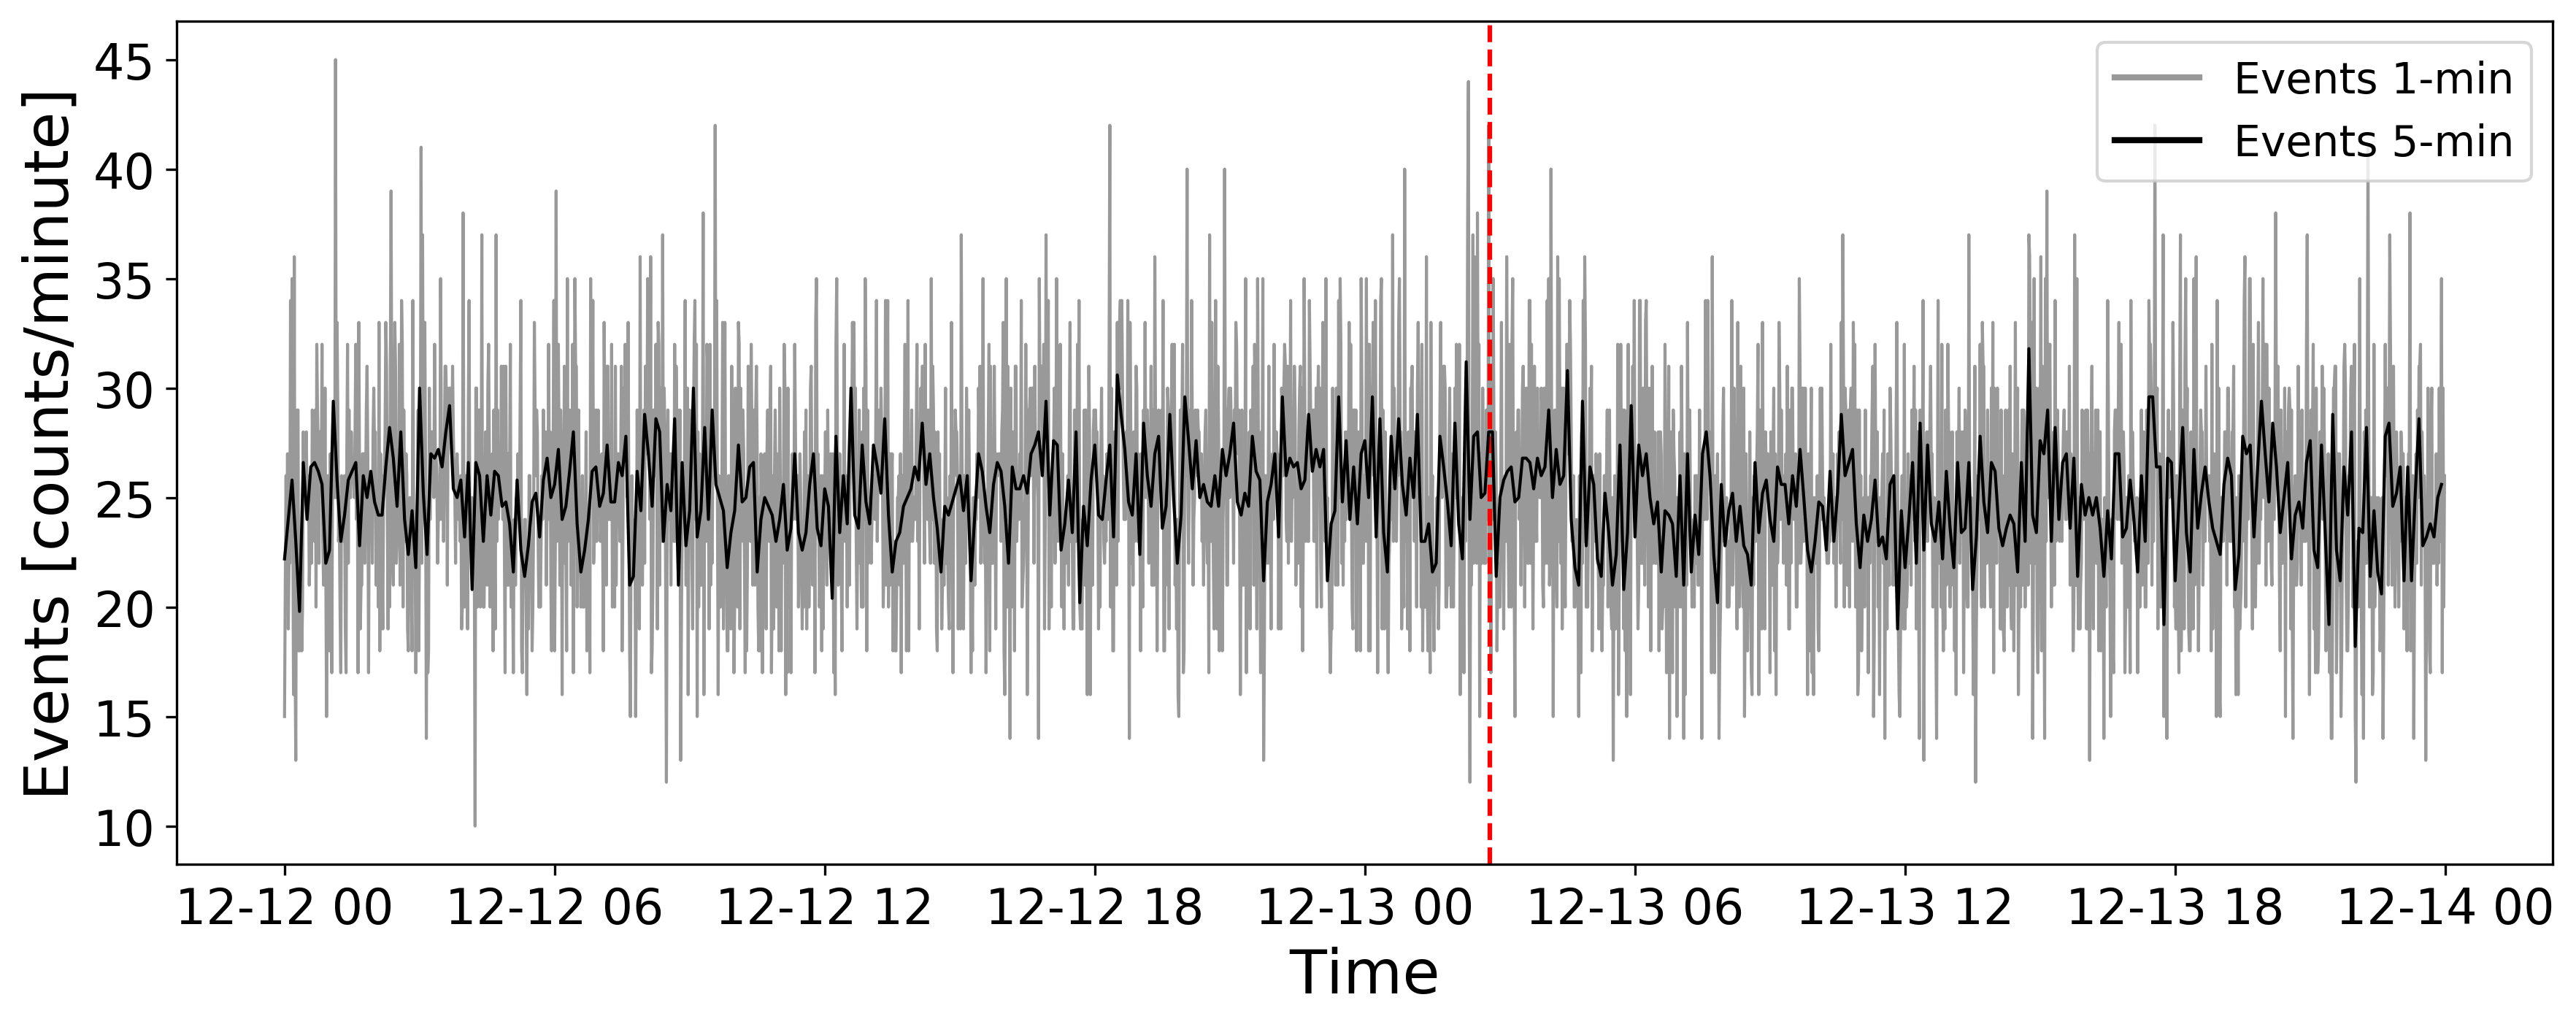
\includegraphics[width=0.48\columnwidth]{GLE70_3001.png}
		\label{fig:GLE70_3001}}
	
	\caption{HiSPARC data for stations 501 and 3001 around the epoch of GLE 70. The plot shows the minute-averaged and 5-minute-averaged trigger events between detectors within the station. The vertical red, dashed line depicts the approximate onset time of the GLE.}
	\label{fig:GLE_70}
\end{figure}


Figure~\ref{fig:GLE_71}...

\begin{figure}[h]
	\centering
	\subfloat[HS 8001 (Eindhoven)]{
		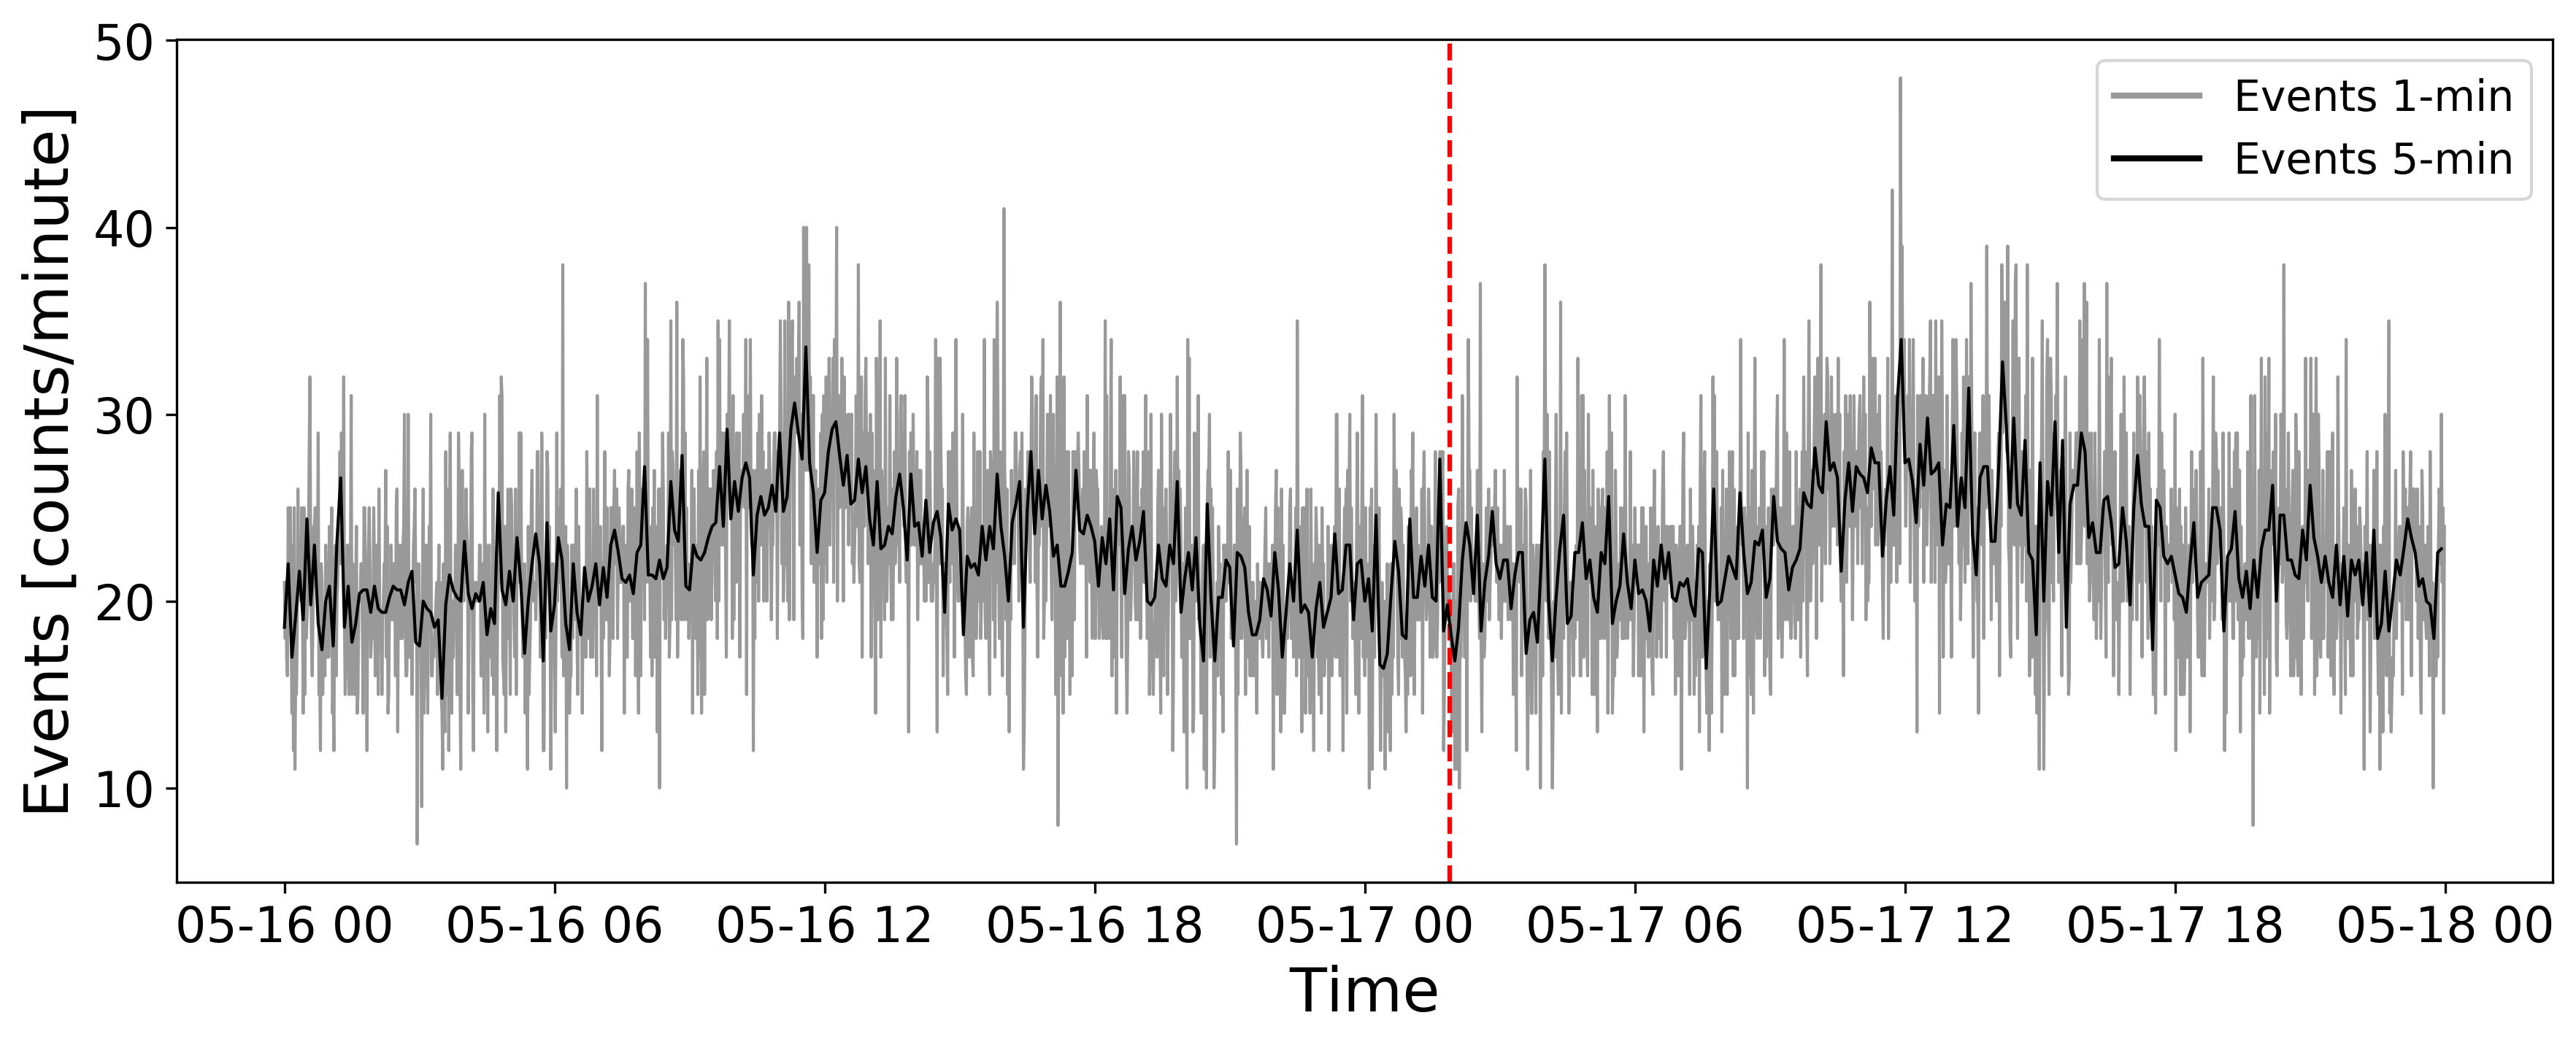
\includegraphics[width=0.48\columnwidth]{GLE71_8001.png}
		\label{fig:GLE71_8001}}
	%\qquad
	\subfloat[HS 3001 (Universiteit Leiden)]{
		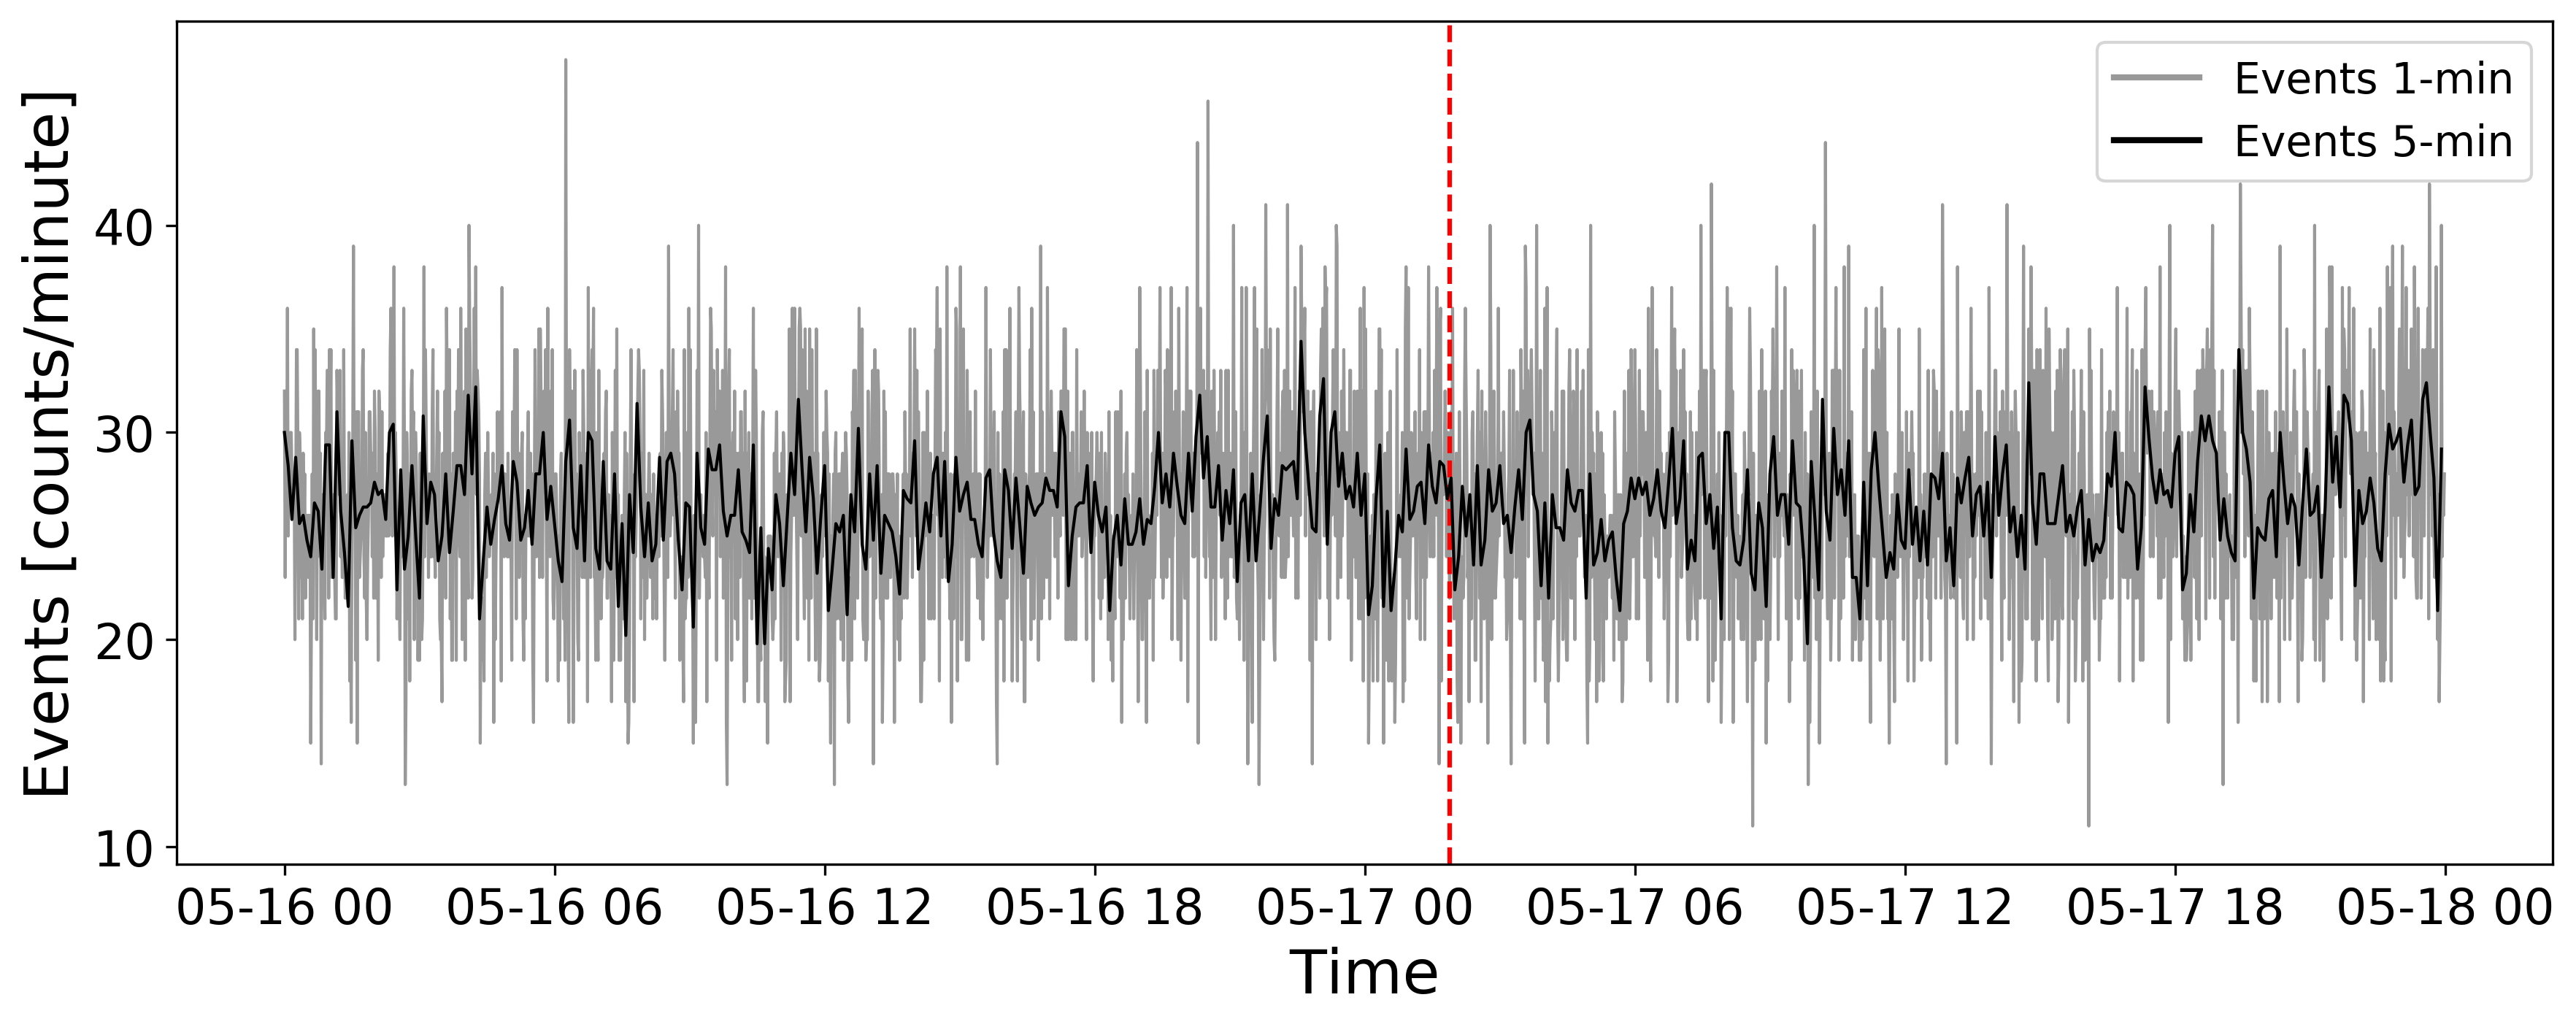
\includegraphics[width=0.48\columnwidth]{GLE71_3001.png}
		\label{fig:GLE71_3001}}
	
	\caption{HiSPARC data for stations 8001 and 3001 around the epoch of GLE 71. The plot shows the minute-averaged and 5-minute-averaged trigger events between detectors within the station. The vertical red, dashed line depicts the approximate onset time of the GLE.}
	\label{fig:GLE_71}
\end{figure}


Figure~\ref{fig:GLE_72}...

\begin{figure}[ht]
	\centering
	\subfloat[HS 501 (Nikhef)]{
		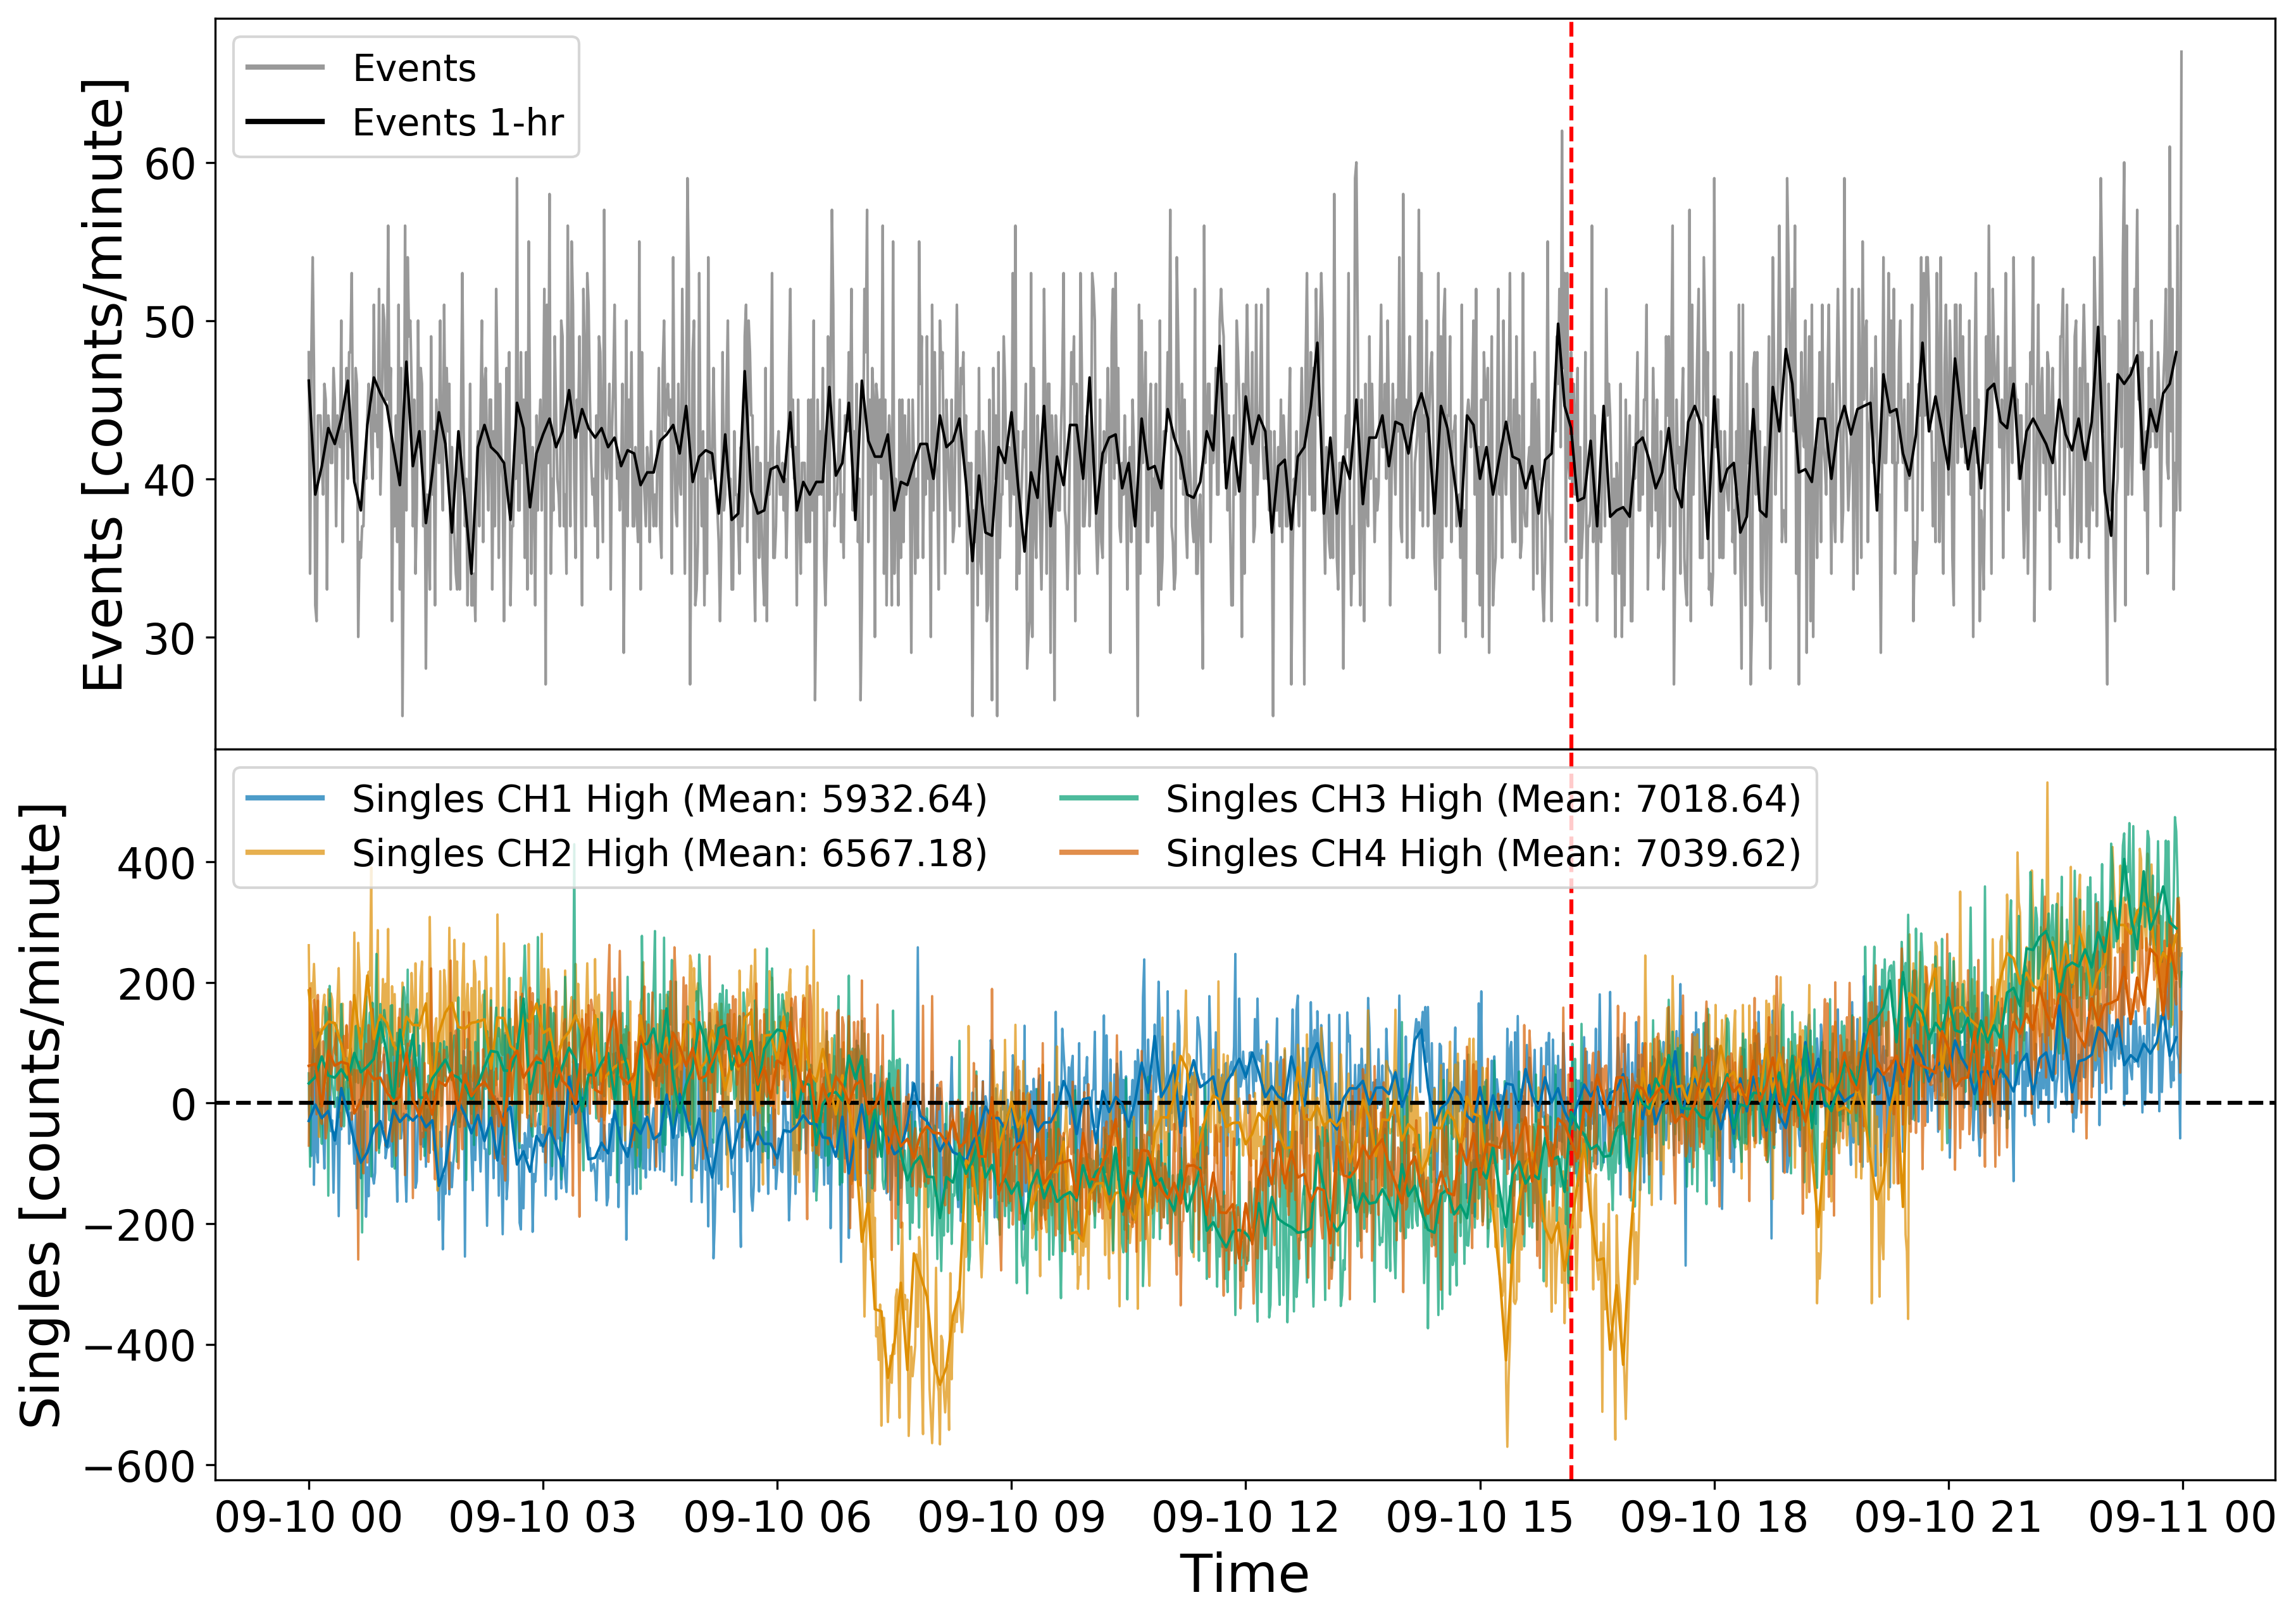
\includegraphics[width=0.48\columnwidth]{GLE72_501.png}
		\label{fig:GLE72_501}}
	%\qquad
	\subfloat[HS 203 (College Hageveld)]{
		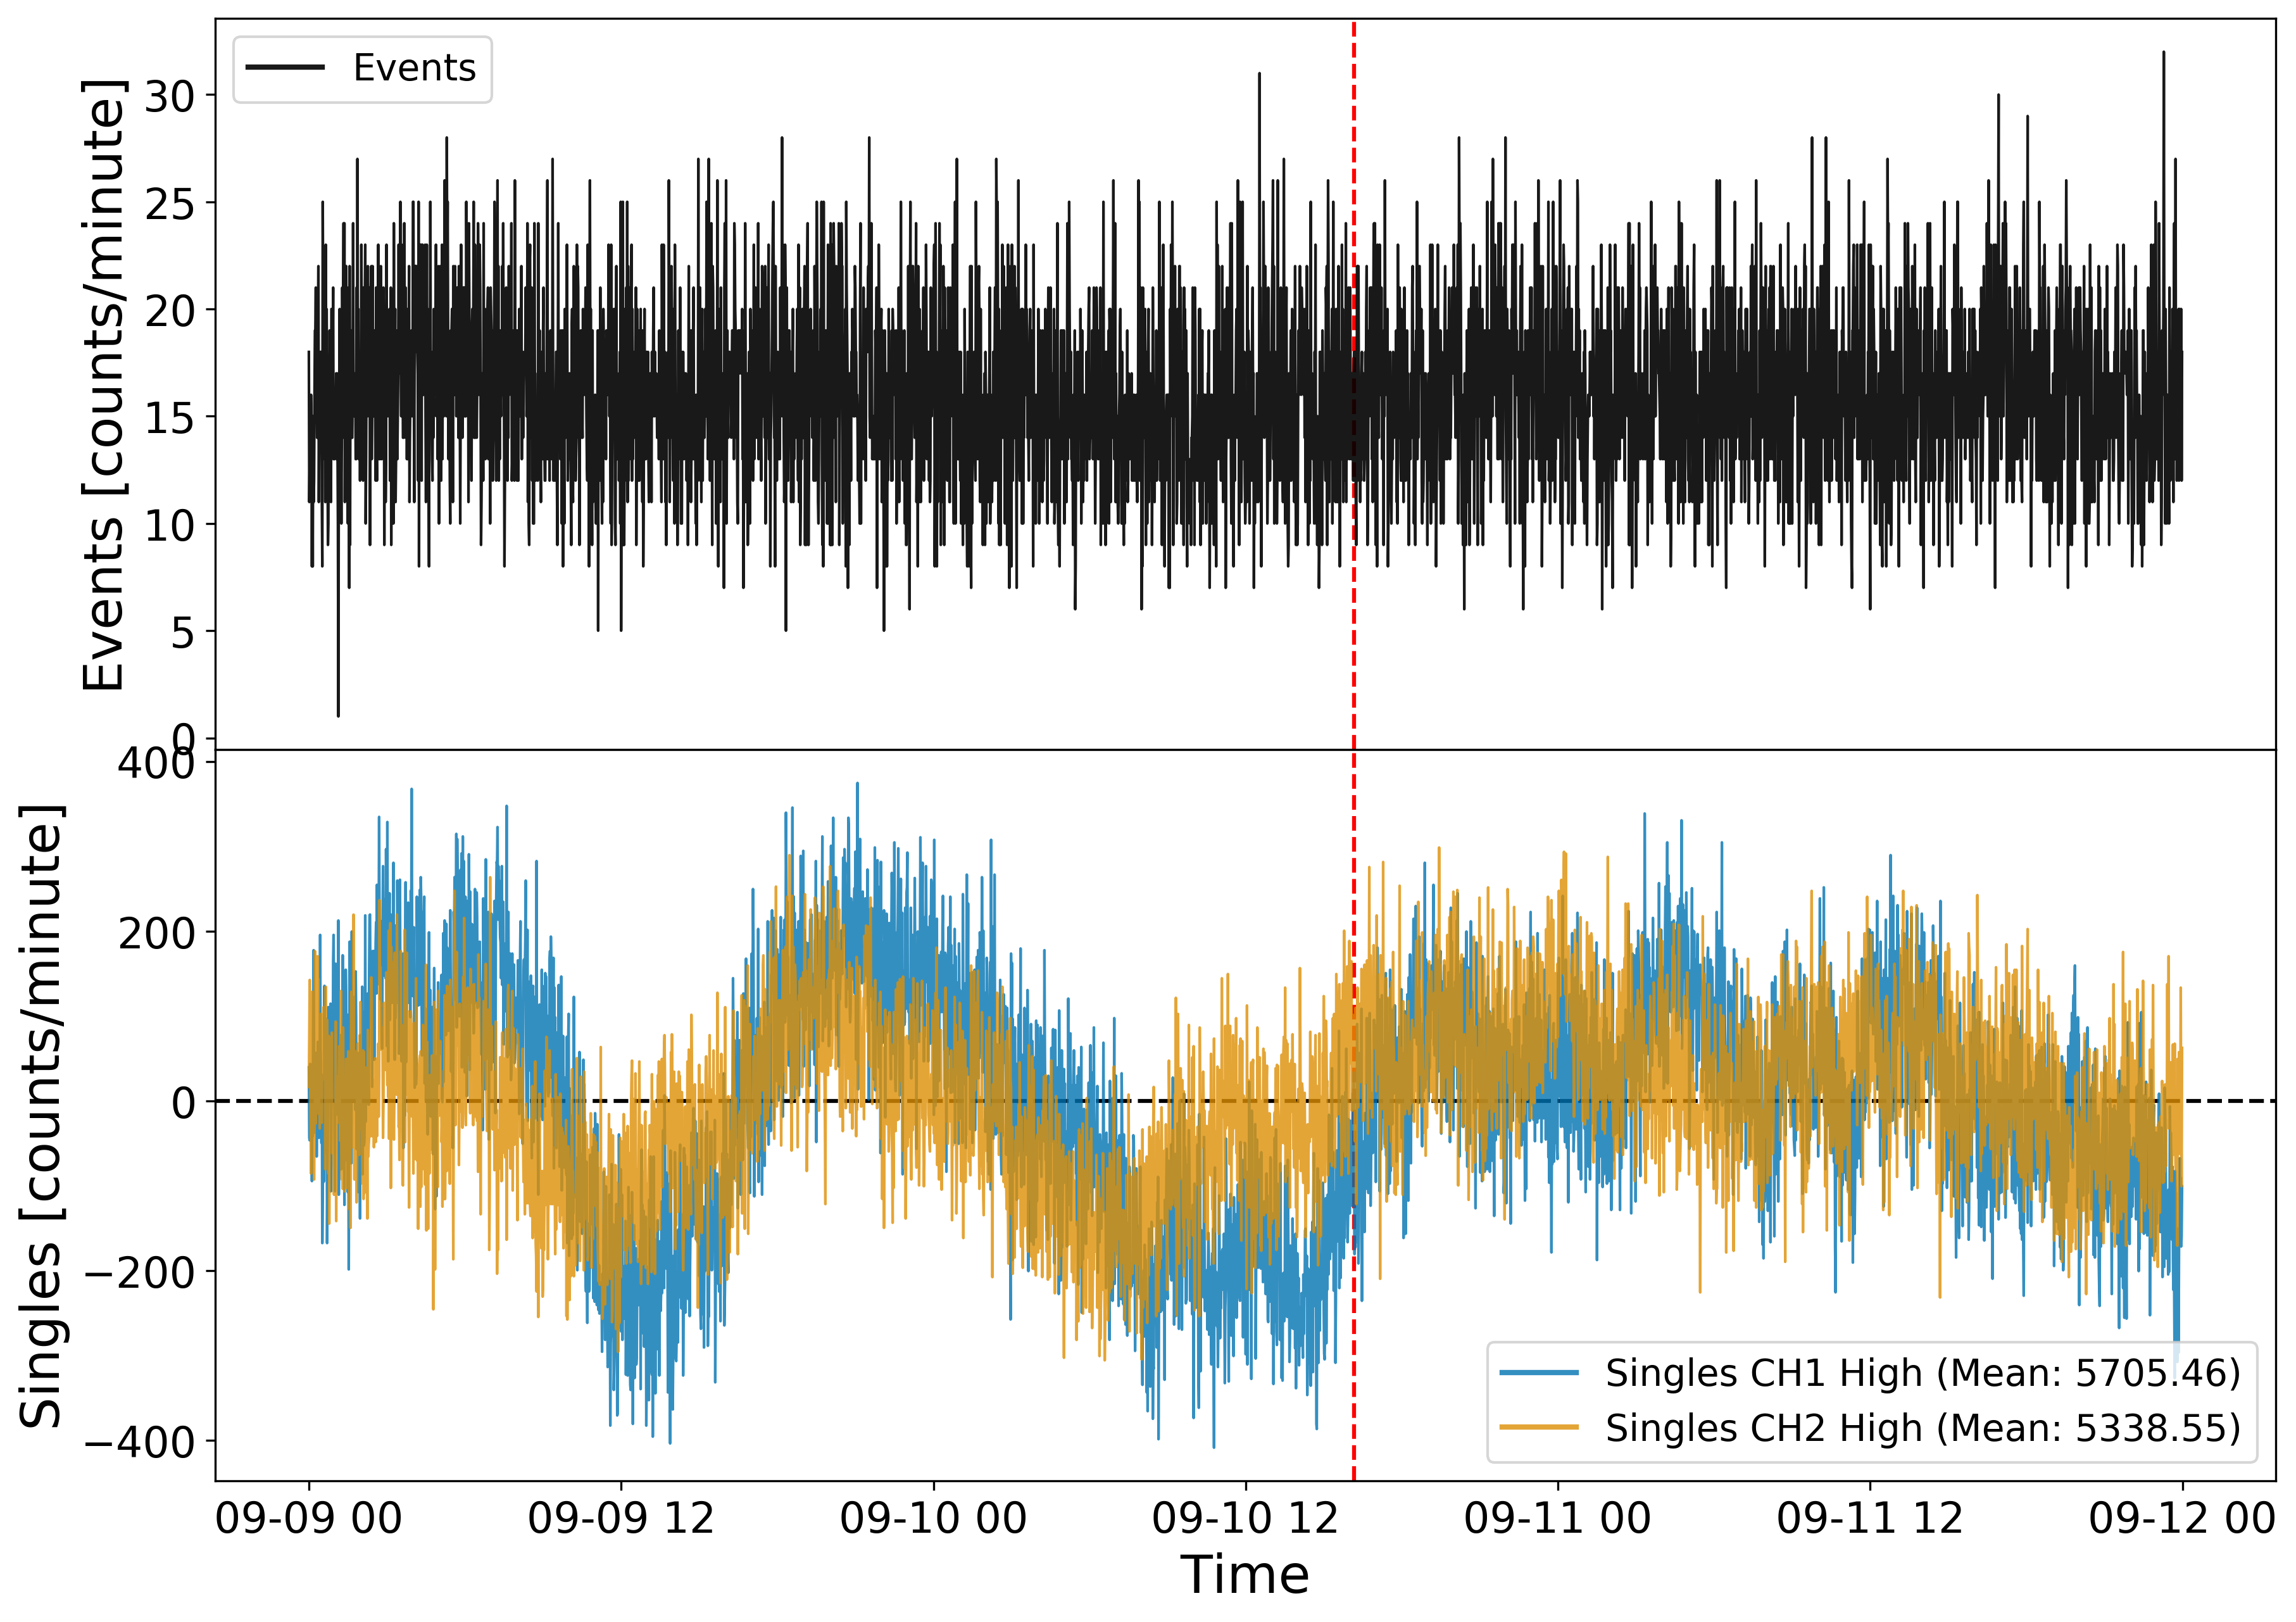
\includegraphics[width=0.48\columnwidth]{GLE72_203.png}
		\label{fig:GLE72_203}} \\
	
	\qquad
	
	\subfloat[HS 8001 (Eindhoven)]{
		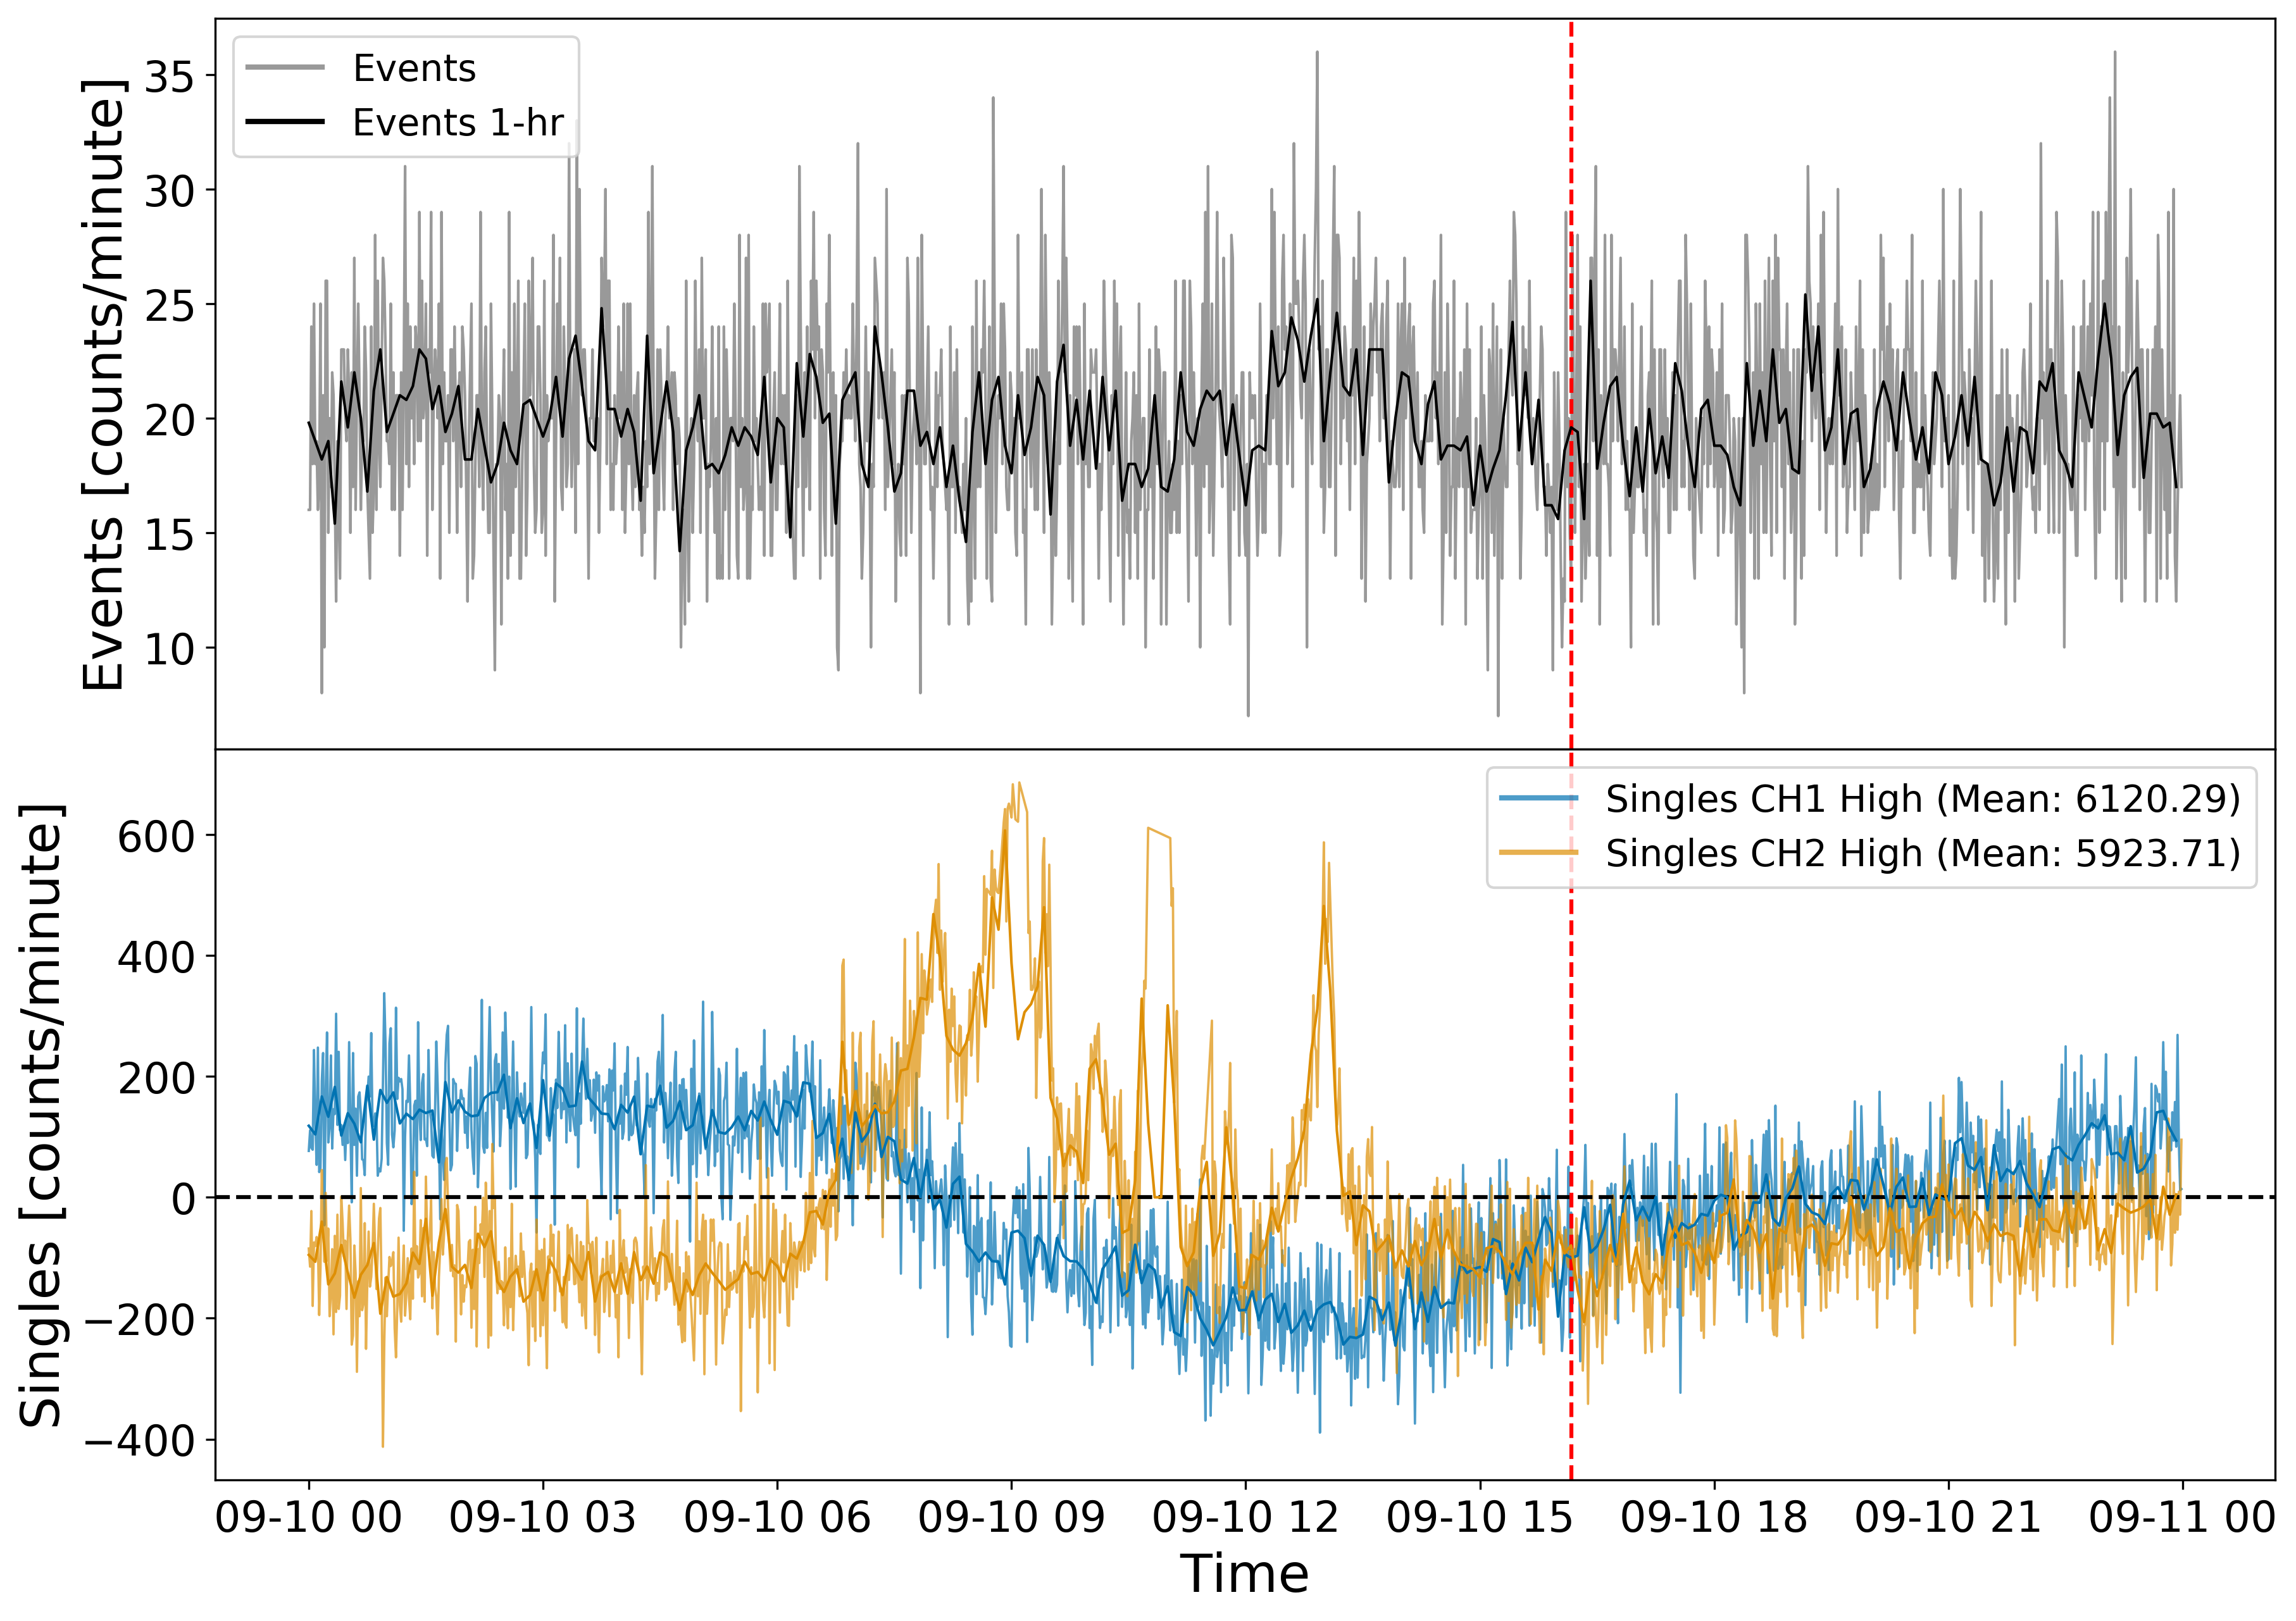
\includegraphics[width=0.48\columnwidth]{GLE72_8001.png}
		\label{fig:GLE72_8001}}
	%\qquad
	\subfloat[HS 14001 (Birmingham University)]{
		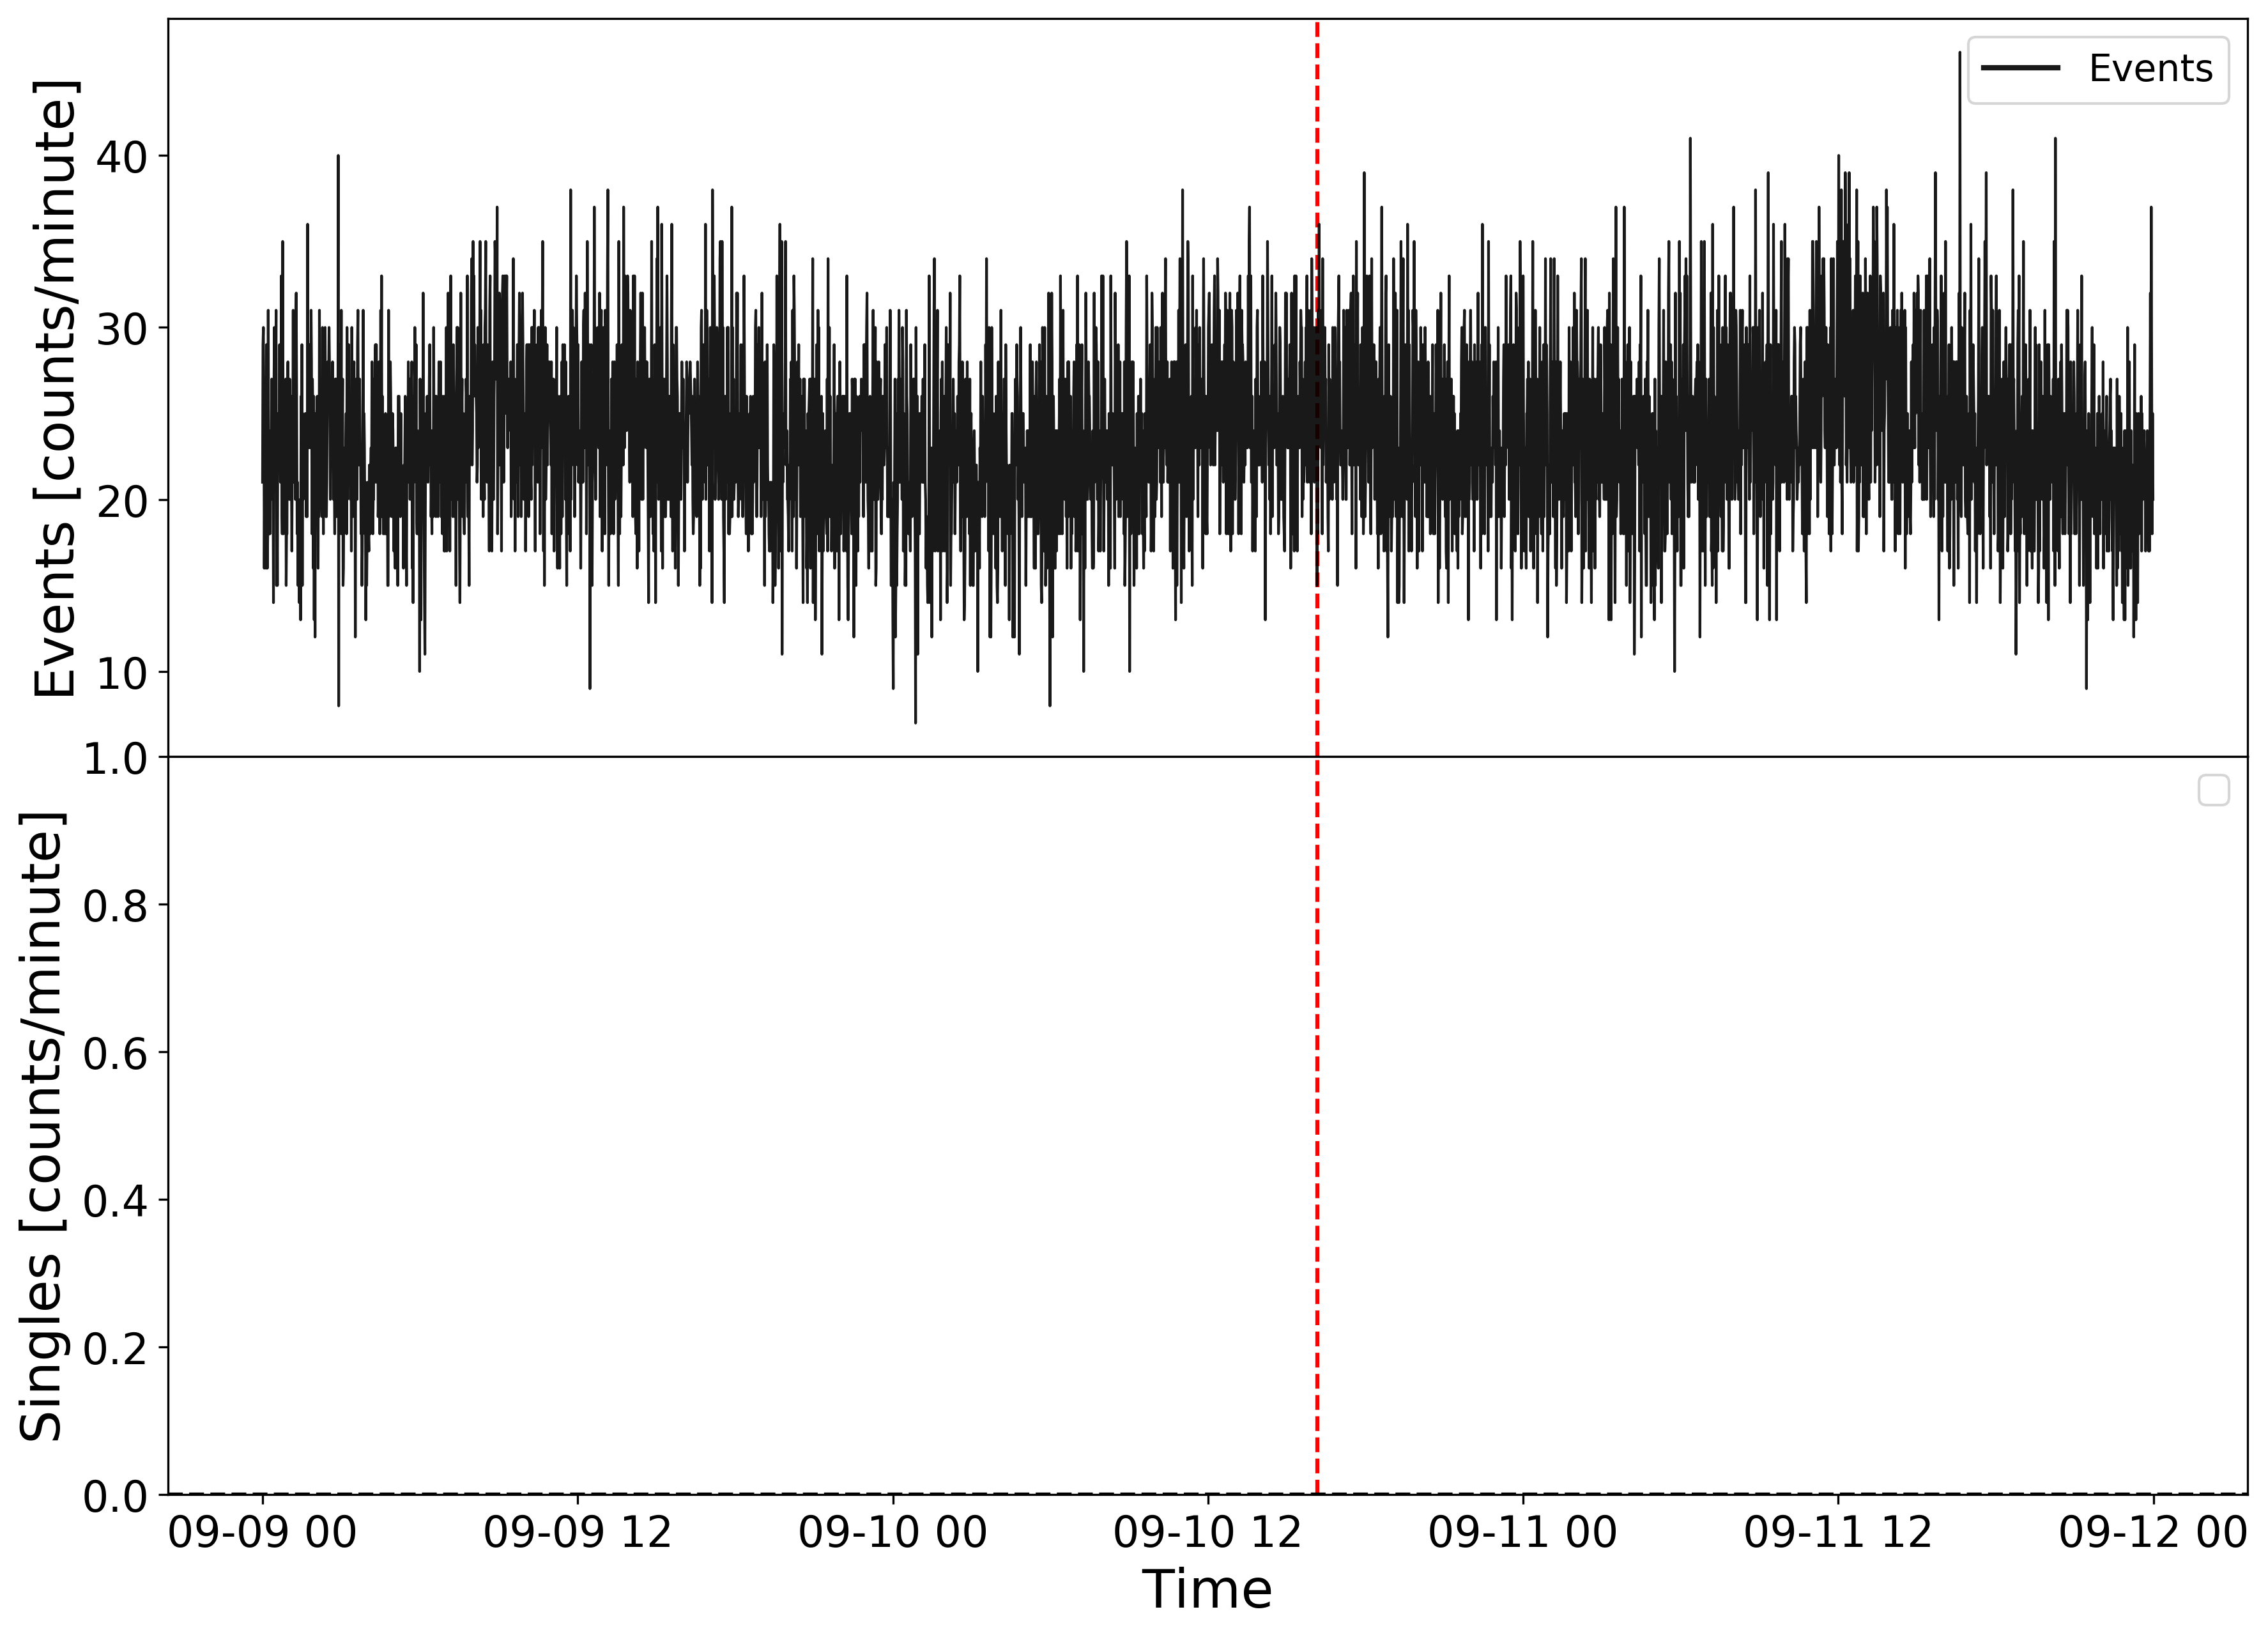
\includegraphics[width=0.48\columnwidth]{GLE72_14001.png}
		\label{fig:GLE72_14001}}
	
	\caption{HiSPARC data for 4 stations around the epoch of GLE 72. The top panel of each subplot shows the minute-averaged trigger events between detectors within the station, while the bottom panel shows the mean-shifted, minute-averaged counts by each individual detector in the station. The vertical red, dashed line depicts the approximate onset time of the GLE.}
	\label{fig:GLE_72}
\end{figure}

... no clear GLE seen...

%%%%%%%%%%%%%%%%%%%%%%%%%%%%%%%%%%%%%%%%%%%%%%%%%%%%%%%%%%%%%%%%%%%%%
\subsection{HiSPARC Observations of Forbush Decreases}

Figure~\ref{fig:FD_201203}...

\begin{figure}[ht]
	\centering
	\subfloat[HS 501 (Nikhef)]{
		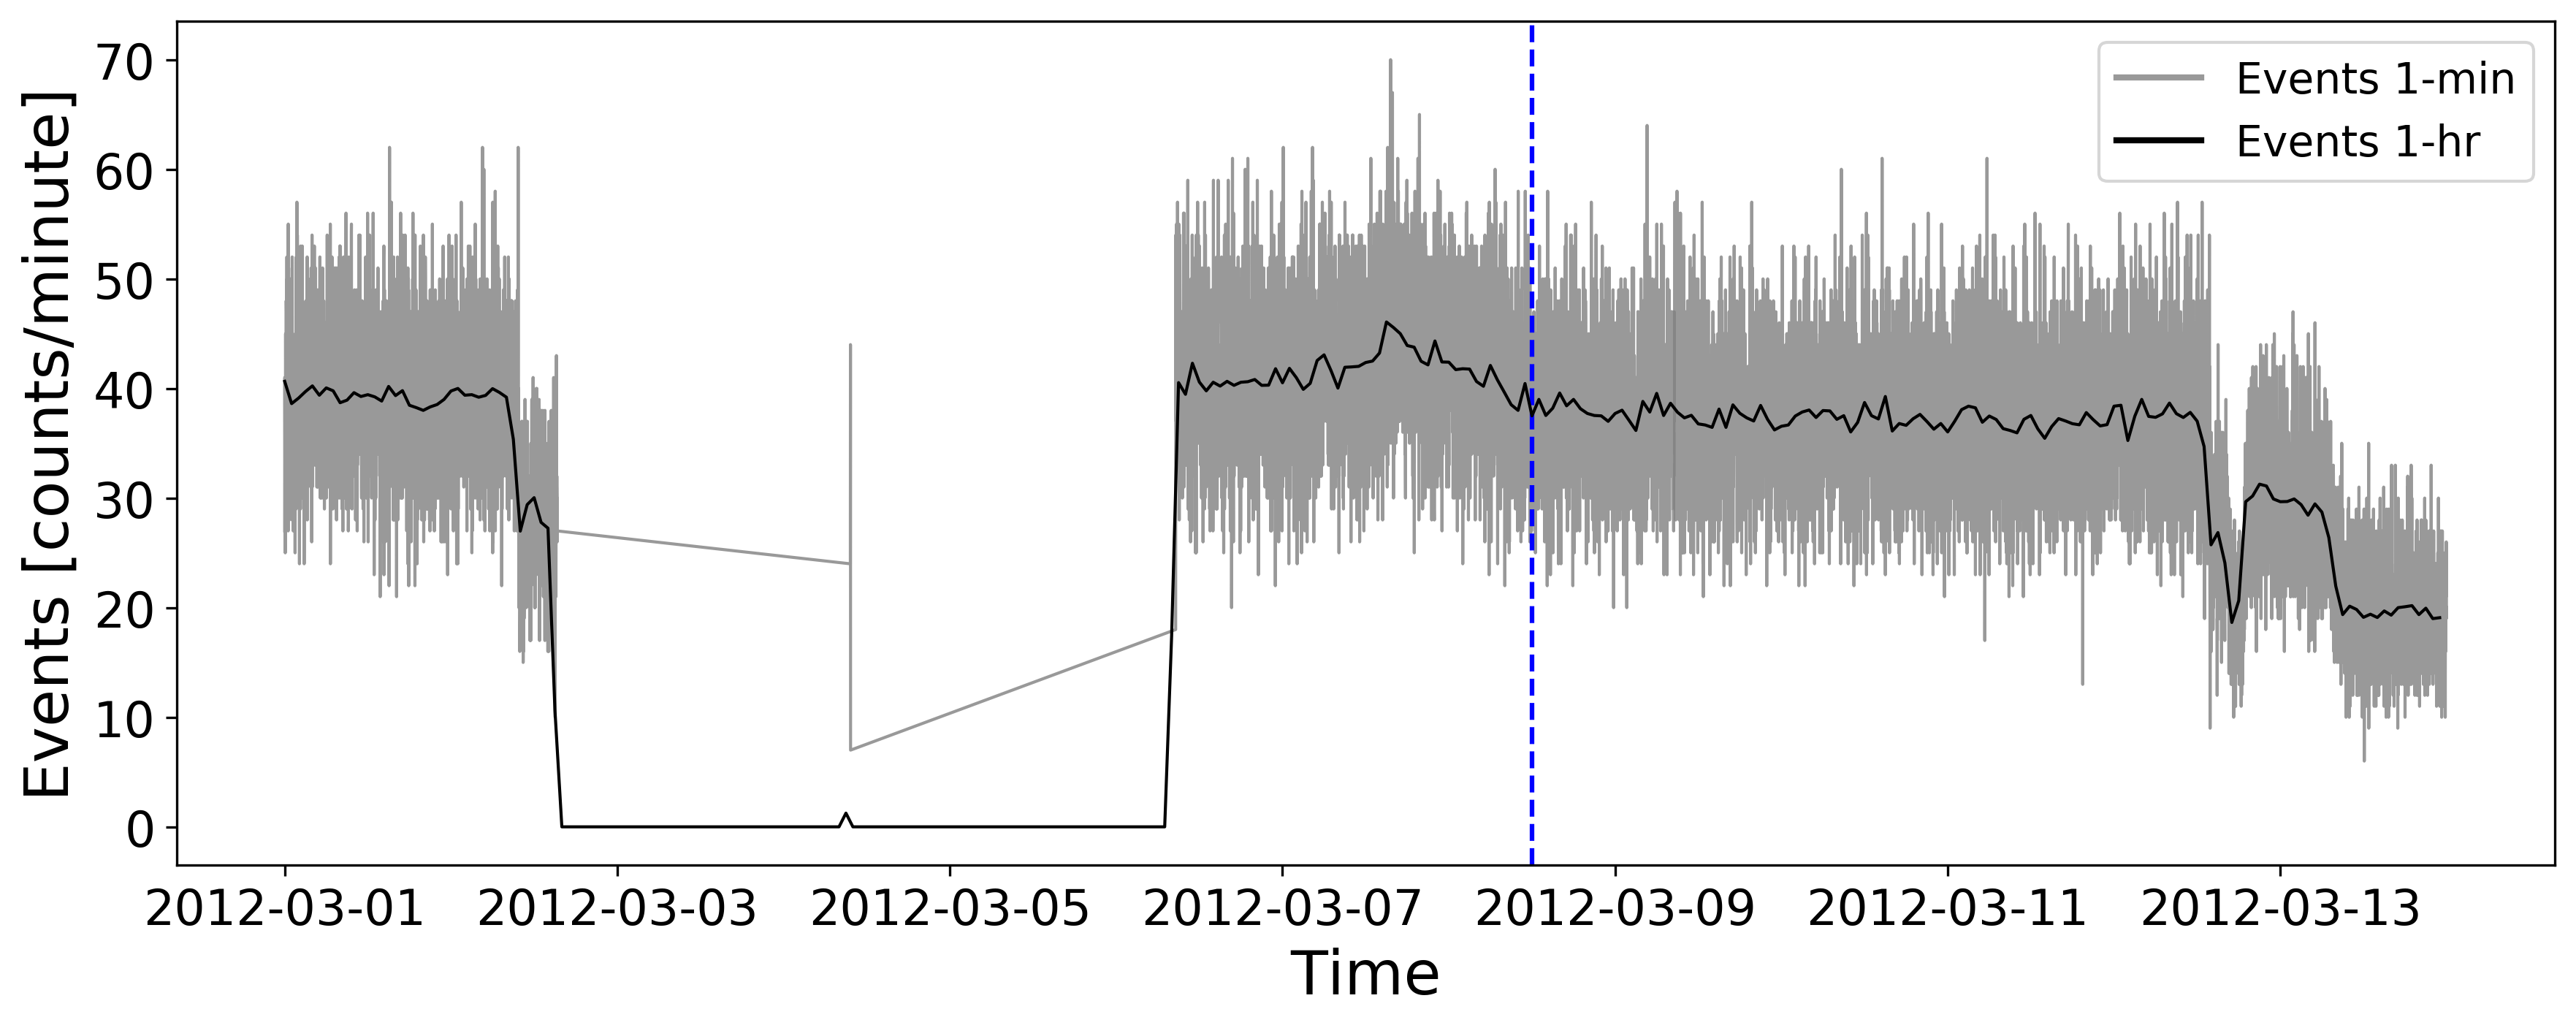
\includegraphics[width=0.48\columnwidth]{FD_201203_501.png}
		\label{fig:FD_201203_501}}
	%\qquad
	\subfloat[HS 8001 (Eindhoven)]{
		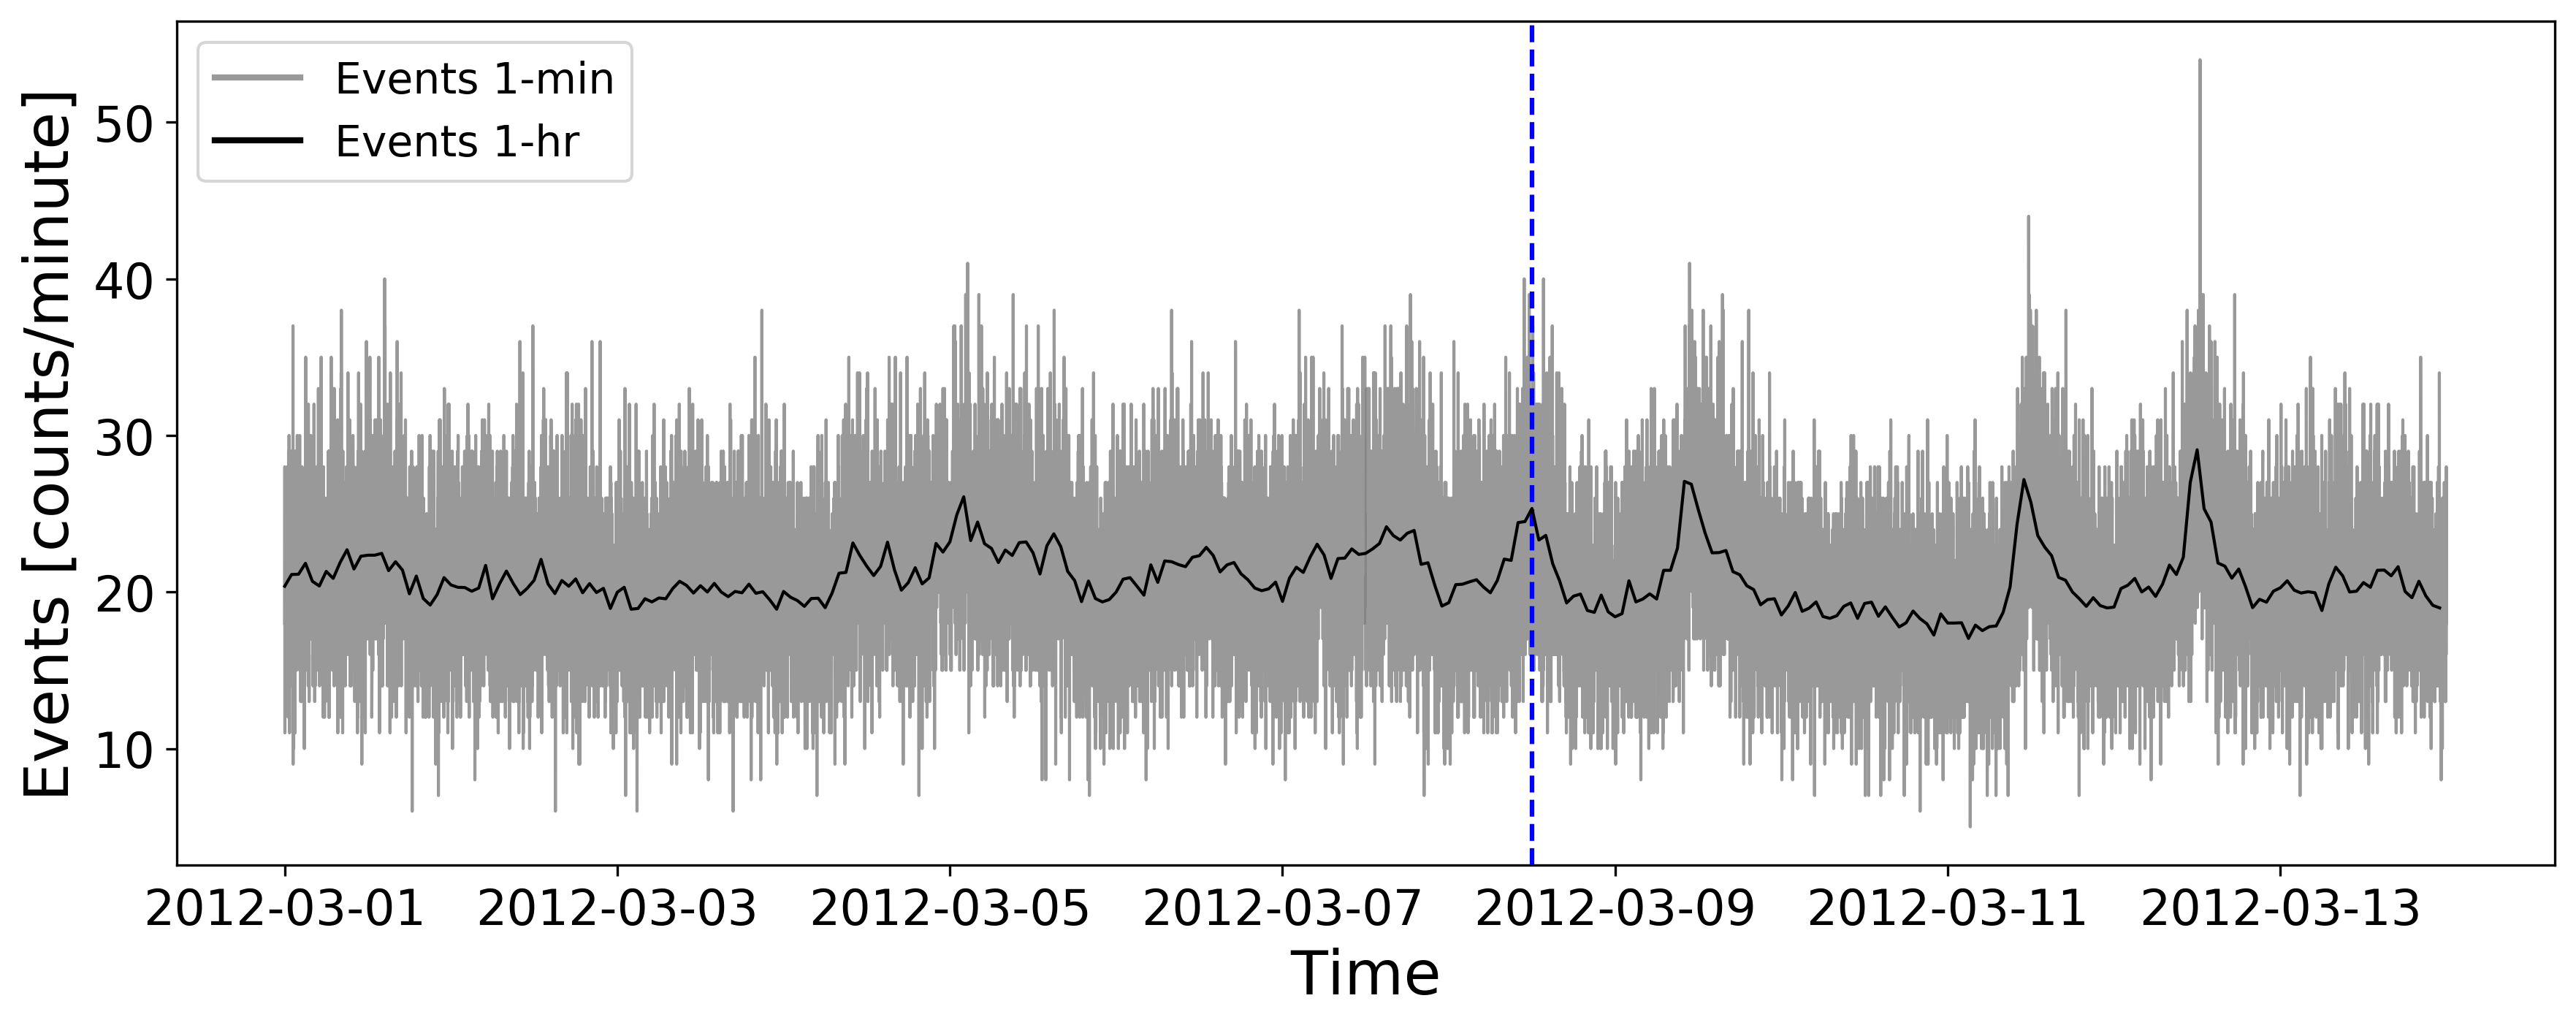
\includegraphics[width=0.48\columnwidth]{FD_201203_8001.png}
		\label{fig:FD_201203_8001}}
	
	\caption{HiSPARC data for stations 501 and 8001 around the epoch of the FD in March 2012. The plot shows the minute-averaged and hourly-averaged trigger events between detectors within the station. The vertical blue-dashed line shows the approximate onset-time of the FD.}
	\label{fig:FD_201203}
\end{figure}


Figure~\ref{fig:FD_201207}...

\begin{figure}[ht]
	\centering
	\subfloat[HS 501 (Nikhef)]{
		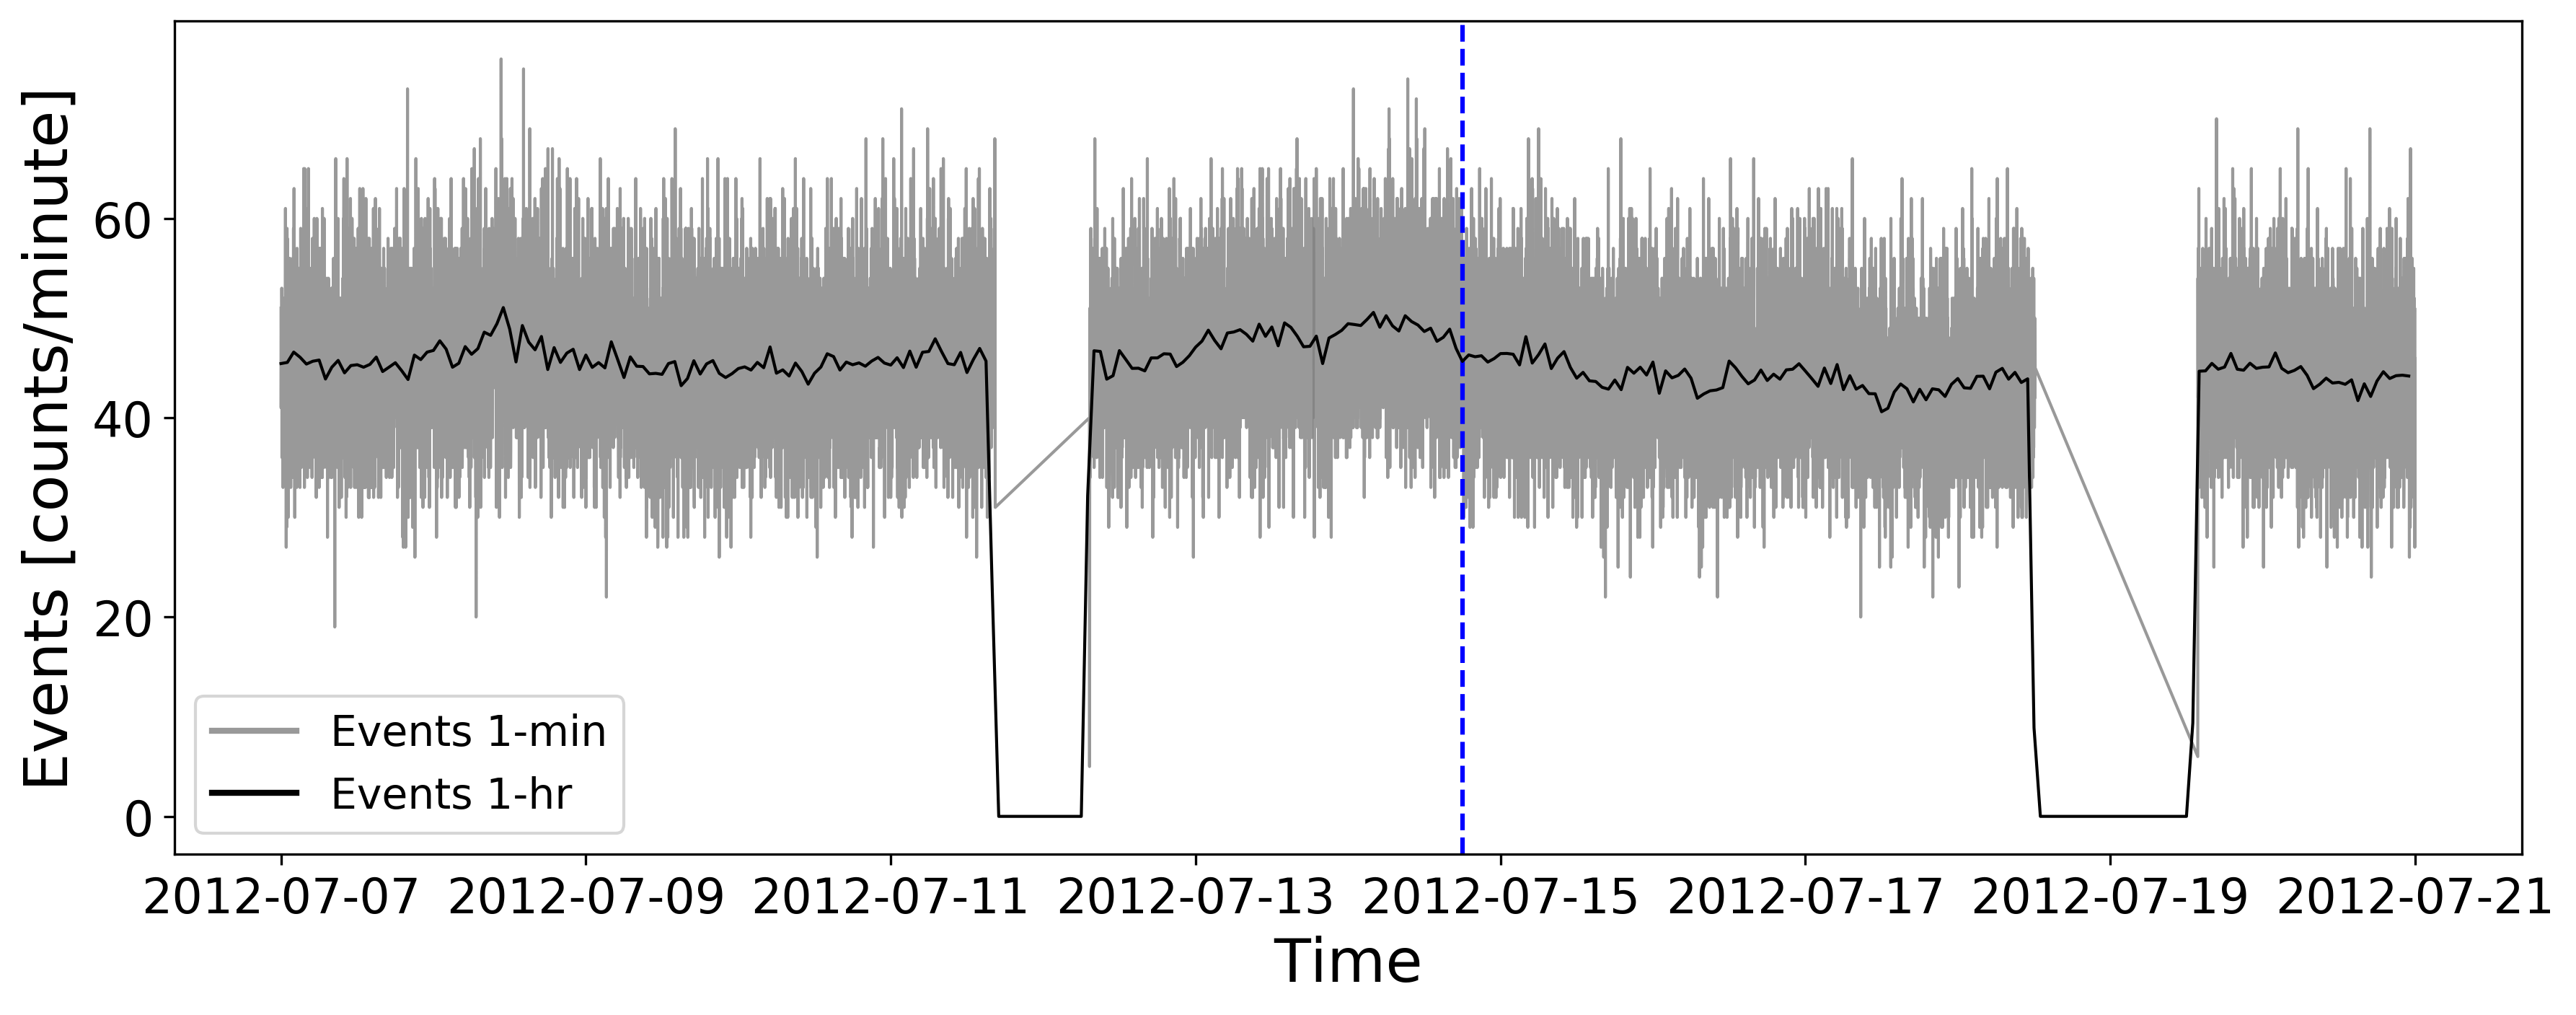
\includegraphics[width=0.48\columnwidth]{FD_201207_501.png}
		\label{fig:FD_201207_501}}
	%\qquad
	\subfloat[HS 8001 (Eindhoven)]{
		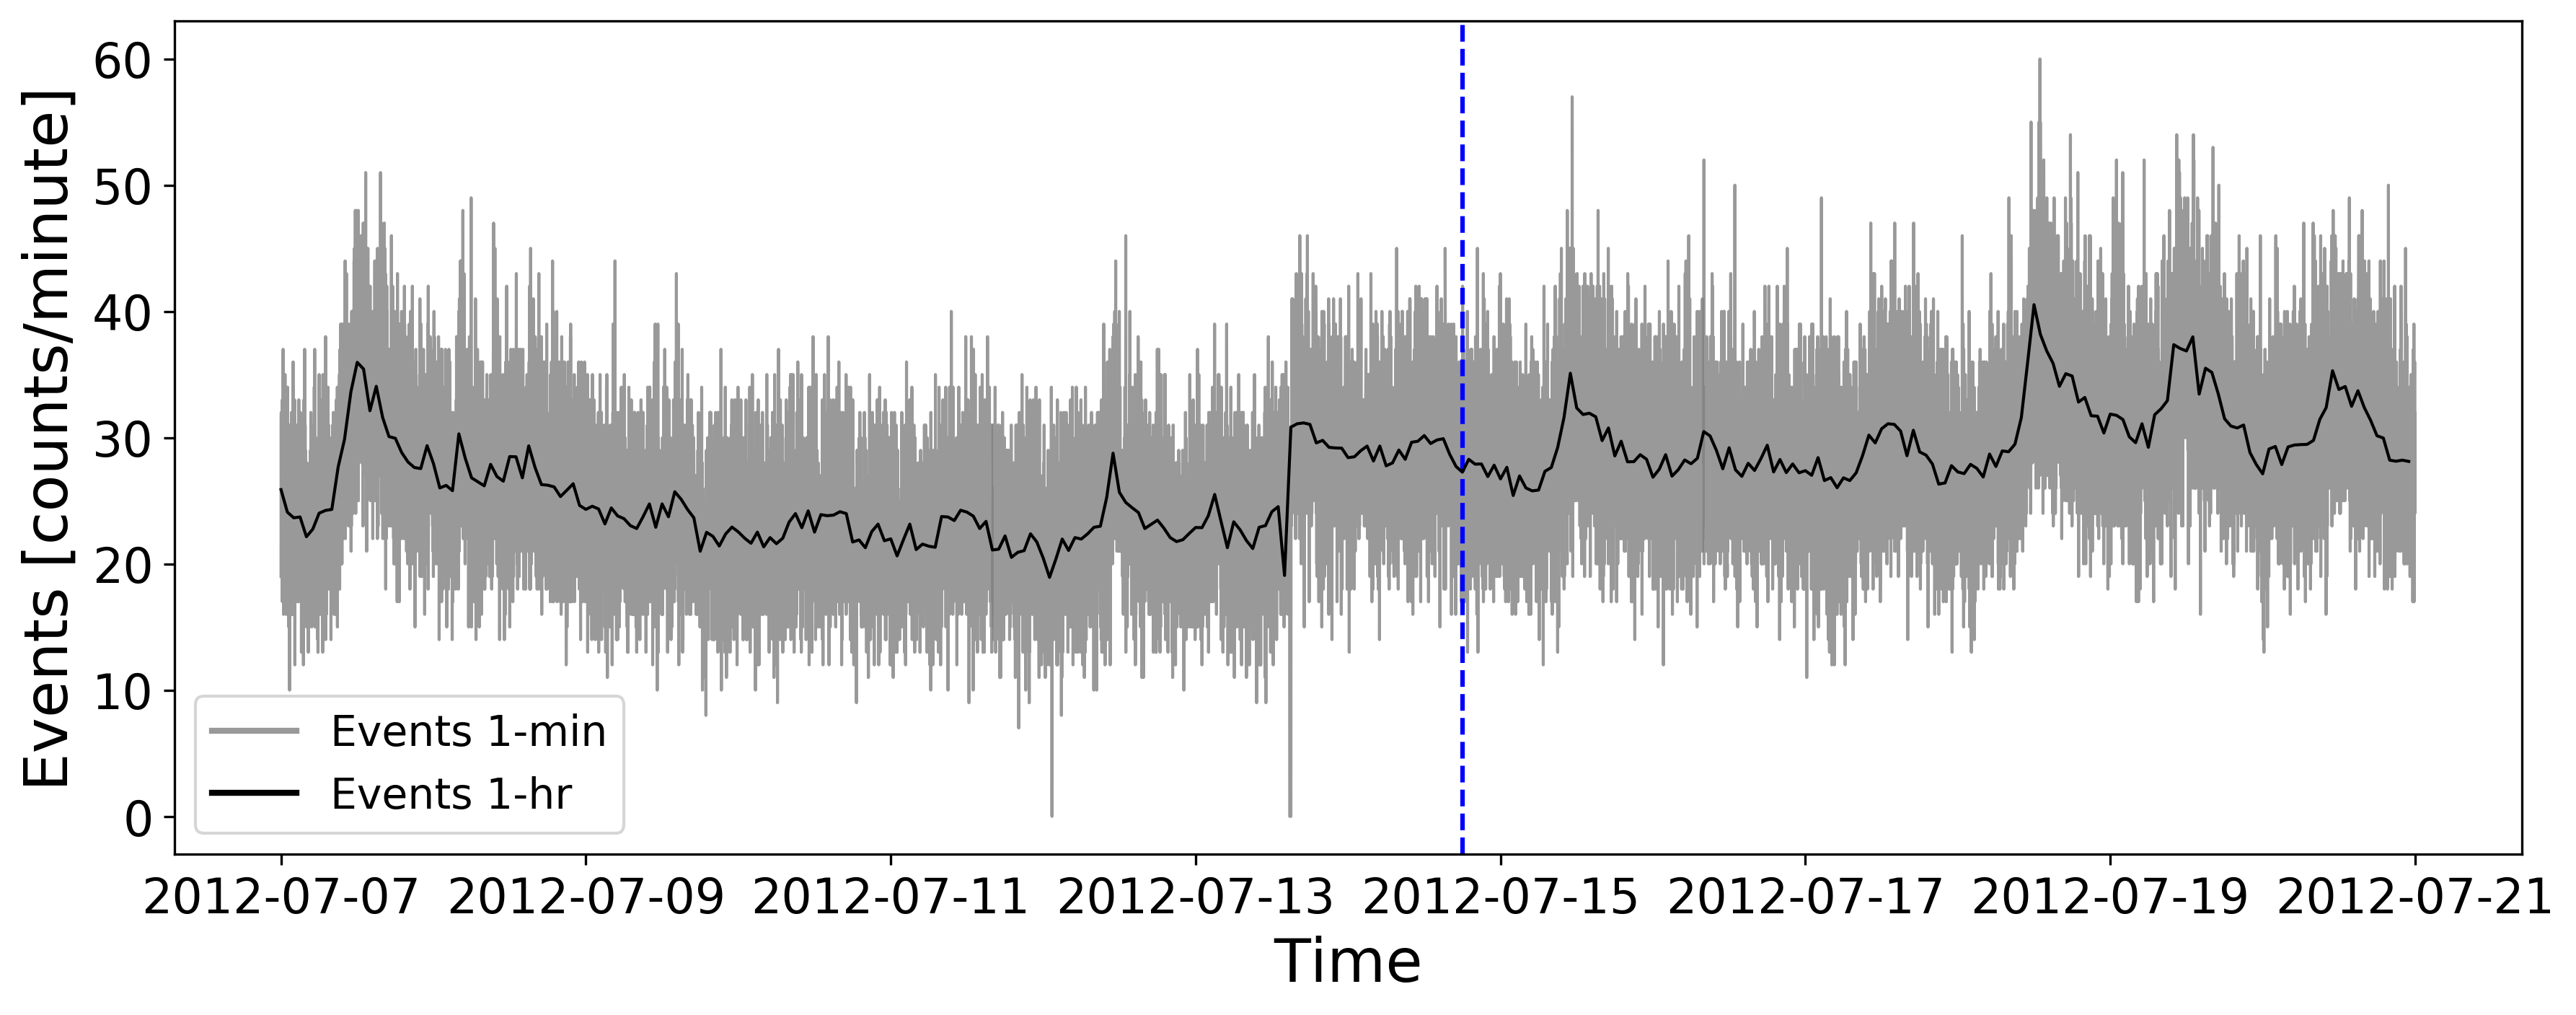
\includegraphics[width=0.48\columnwidth]{FD_201207_8001.png}
		\label{fig:FD_201207_8001}}
	
	\caption{HiSPARC data for stations 501 and 8001 around the epoch of the FD in July 2012. The plot shows the minute-averaged and hourly-averaged trigger events between detectors within the station. The vertical blue-dashed line shows the approximate onset-time of the FD.}
	\label{fig:FD_201207}
\end{figure}



Figure~\ref{fig:FD_201412}...

\begin{figure}[ht]
	\centering
	\subfloat[HS 501 (Nikhef)]{
		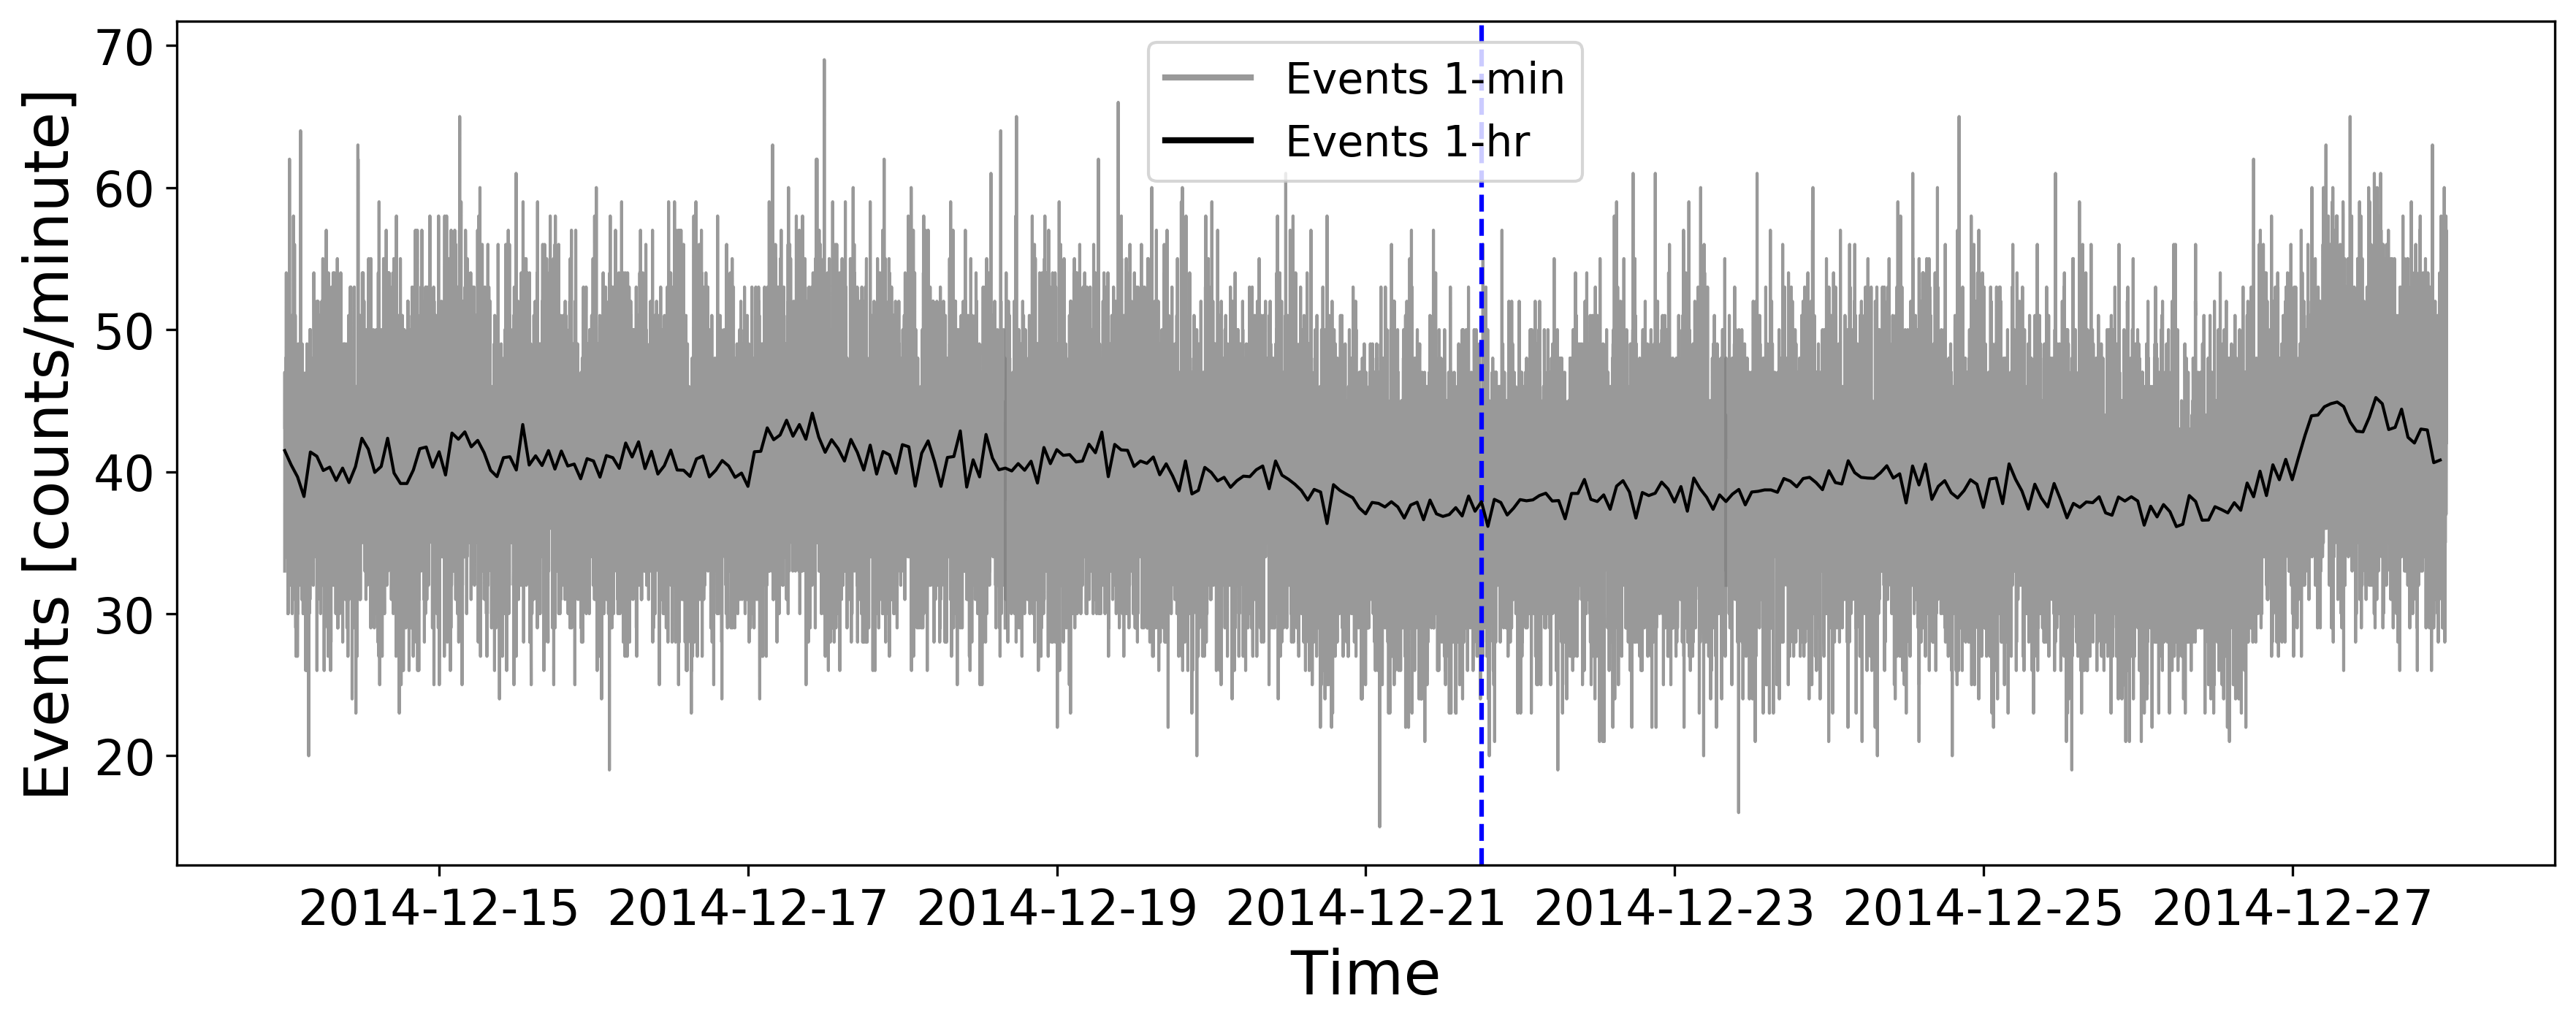
\includegraphics[width=0.48\columnwidth]{FD_201412_501.png}
		\label{fig:FD_201412_501}}
	%\qquad
	\subfloat[HS 203 (College Hageveld)]{
		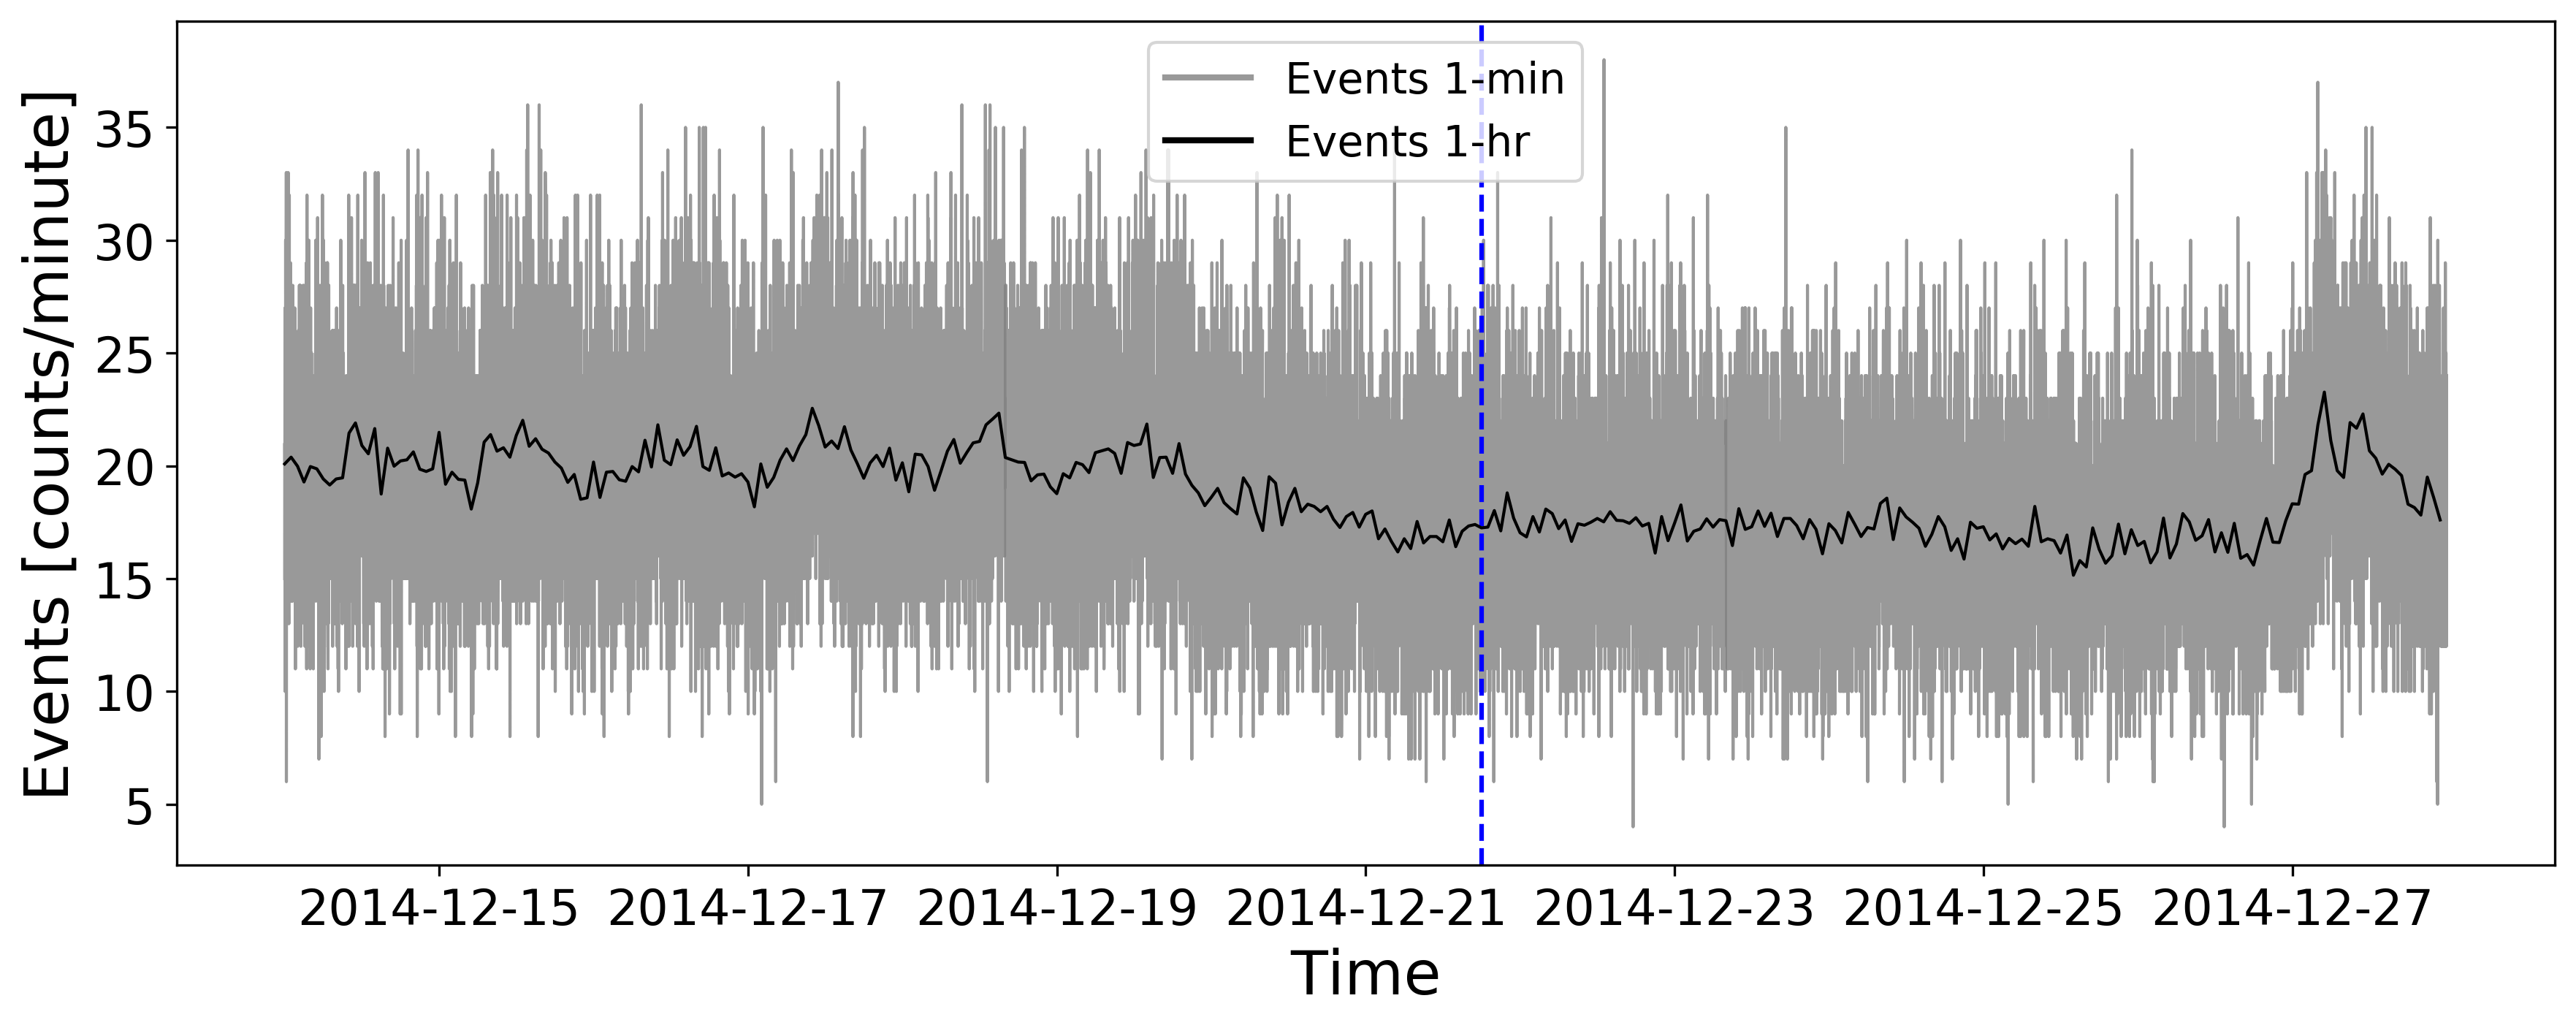
\includegraphics[width=0.48\columnwidth]{FD_201412_203.png}
		\label{fig:FD_201412_203}} \\
	
	\qquad
	
	\subfloat[HS 3001 (Leiden)]{
		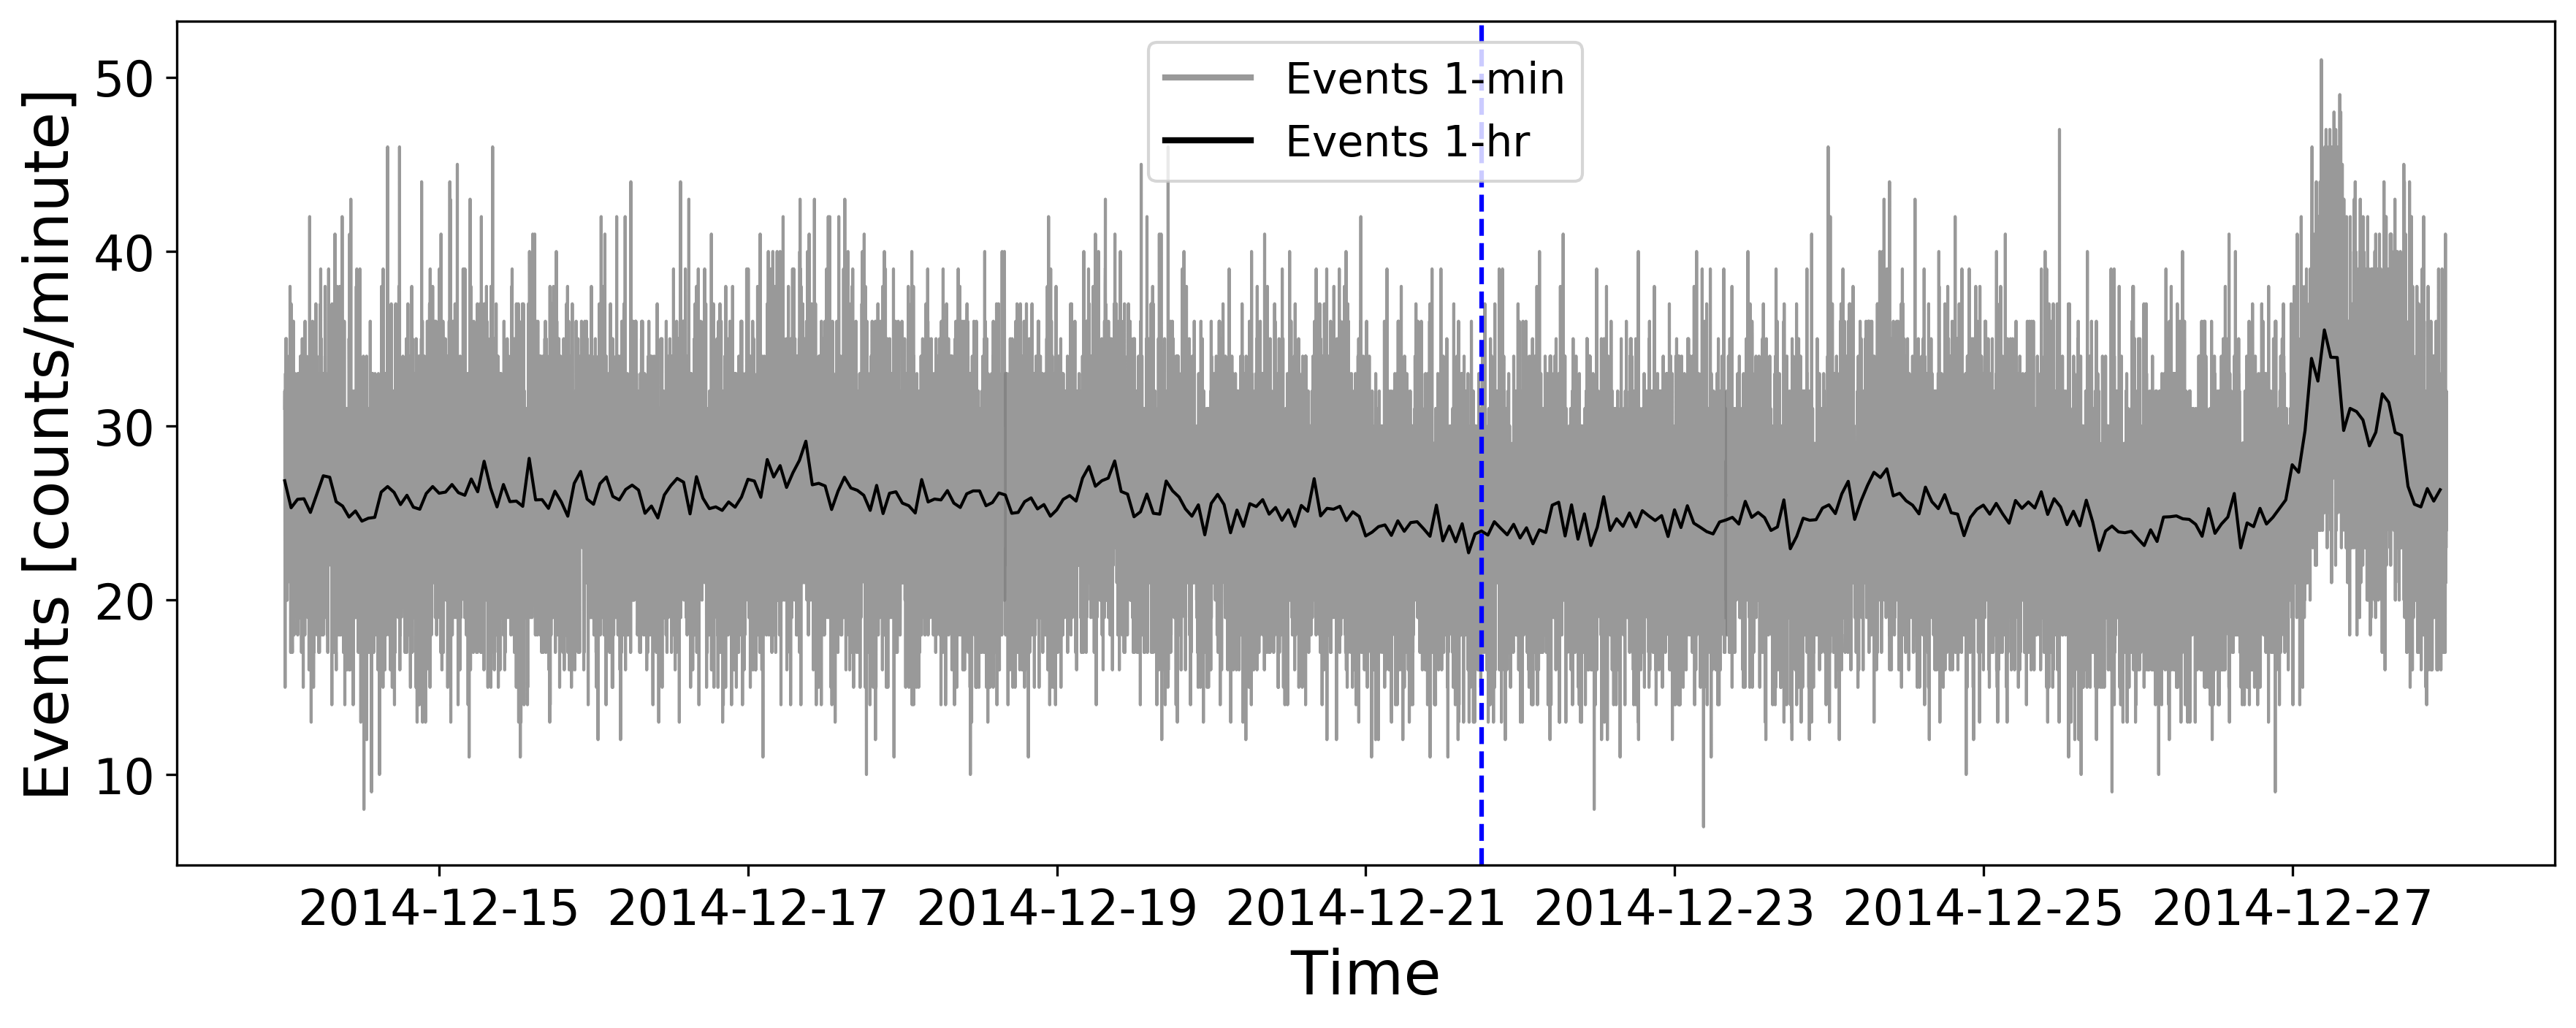
\includegraphics[width=0.48\columnwidth]{FD_201412_3001.png}
		\label{fig:FD_201412_3001}}
	%\qquad
	\subfloat[HS 14001 (Birmingham University)]{
		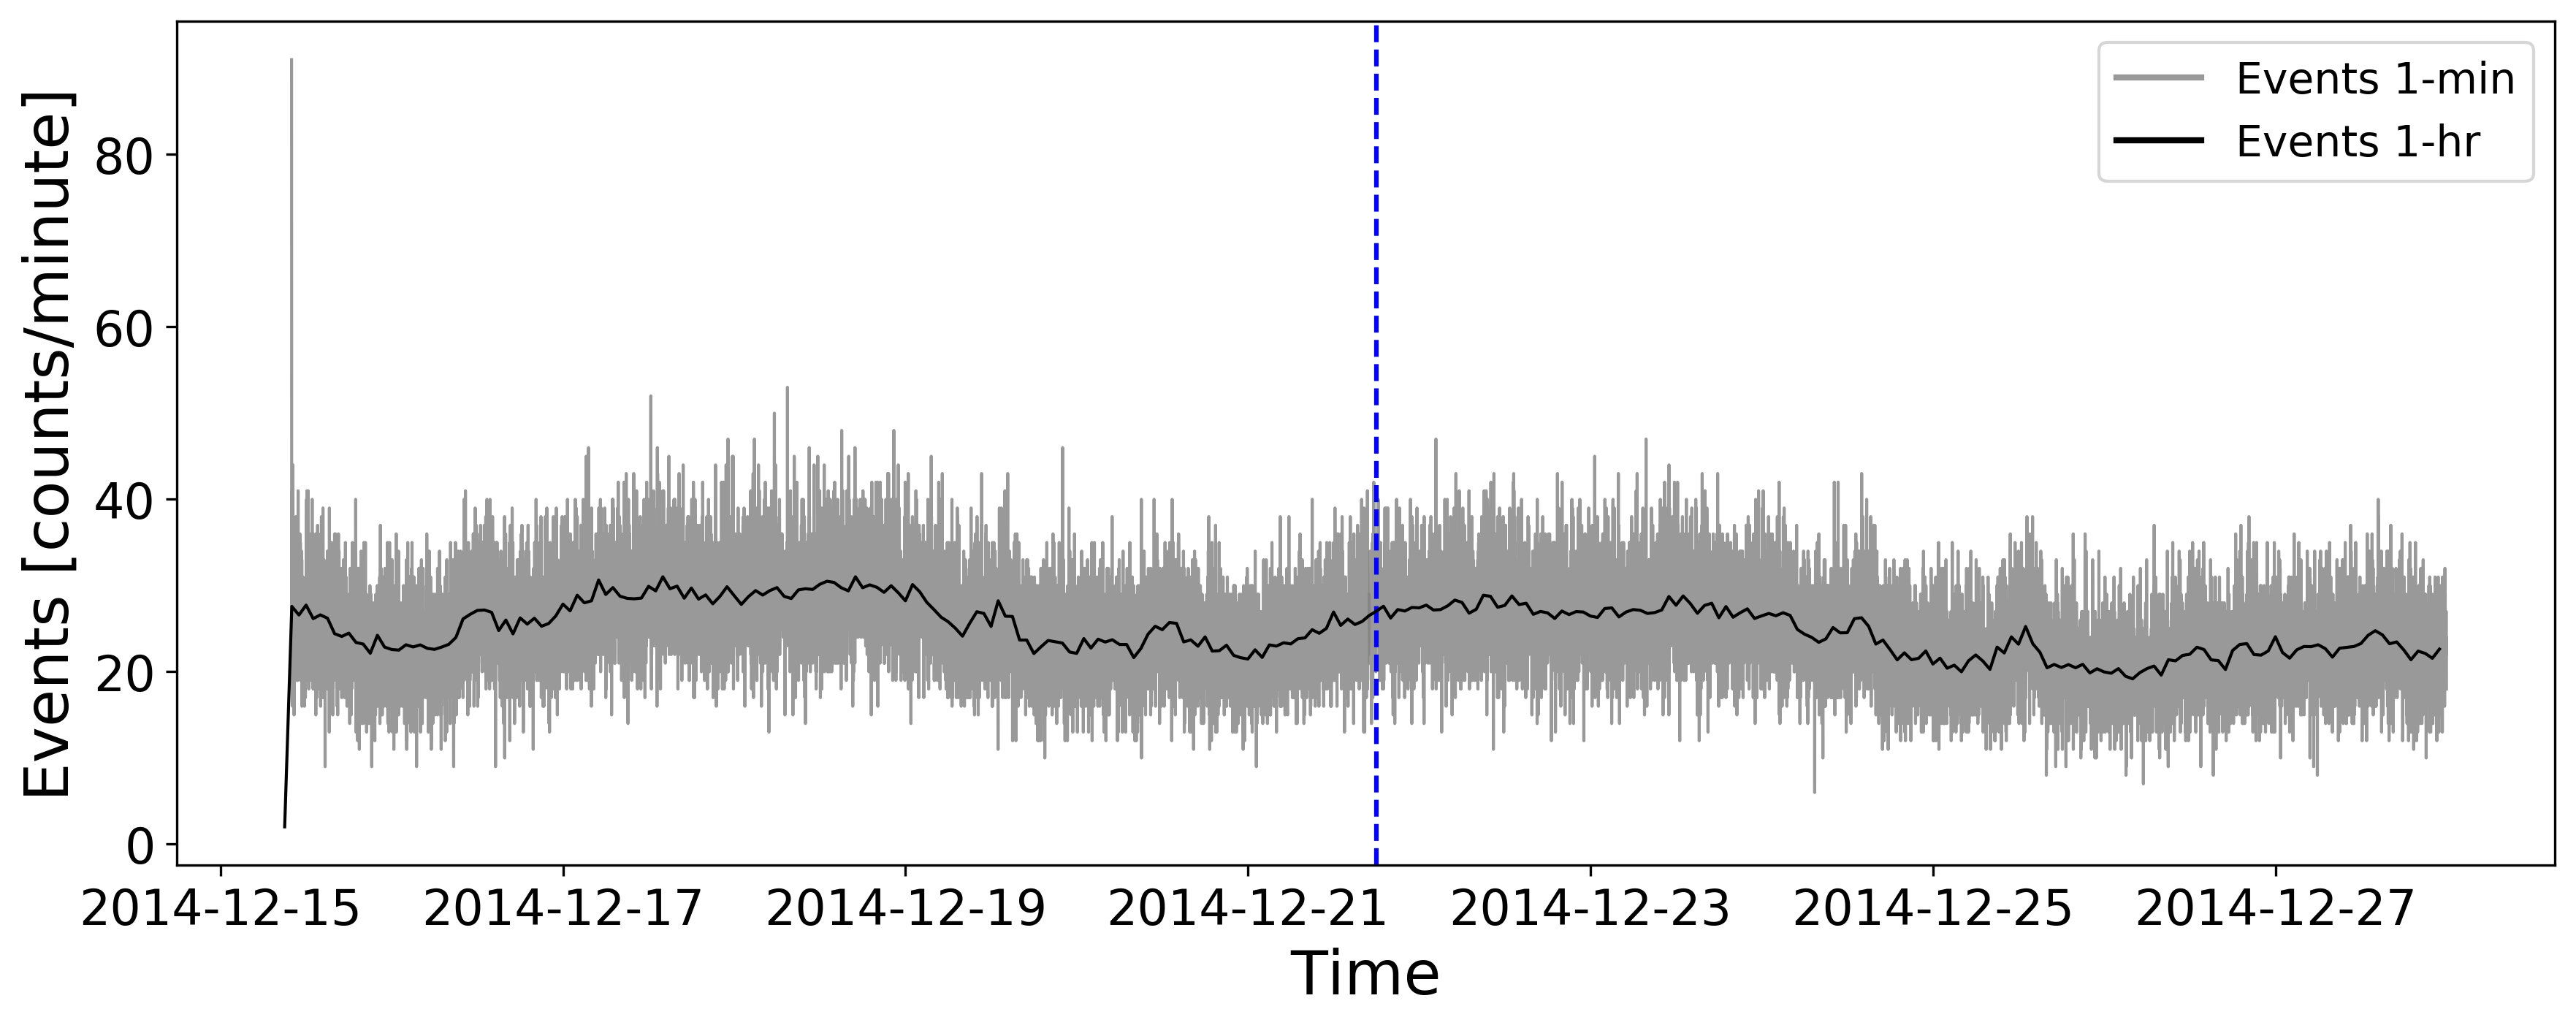
\includegraphics[width=0.48\columnwidth]{FD_201412_14001.png}
		\label{fig:FD_201412_14001}}
	
	\caption{HiSPARC data for 4 stations around the epoch of the FD in December 2014. The plot shows the minute-averaged and hourly-averaged trigger events between detectors within the station. The vertical blue-dashed line shows the approximate onset-time of the FD.}
	\label{fig:FD_201412}
\end{figure}



Figure~\ref{fig:FD_GLE72}...

\begin{figure}[ht]
	\centering
	\subfloat[HS 501 (Nikhef)]{
		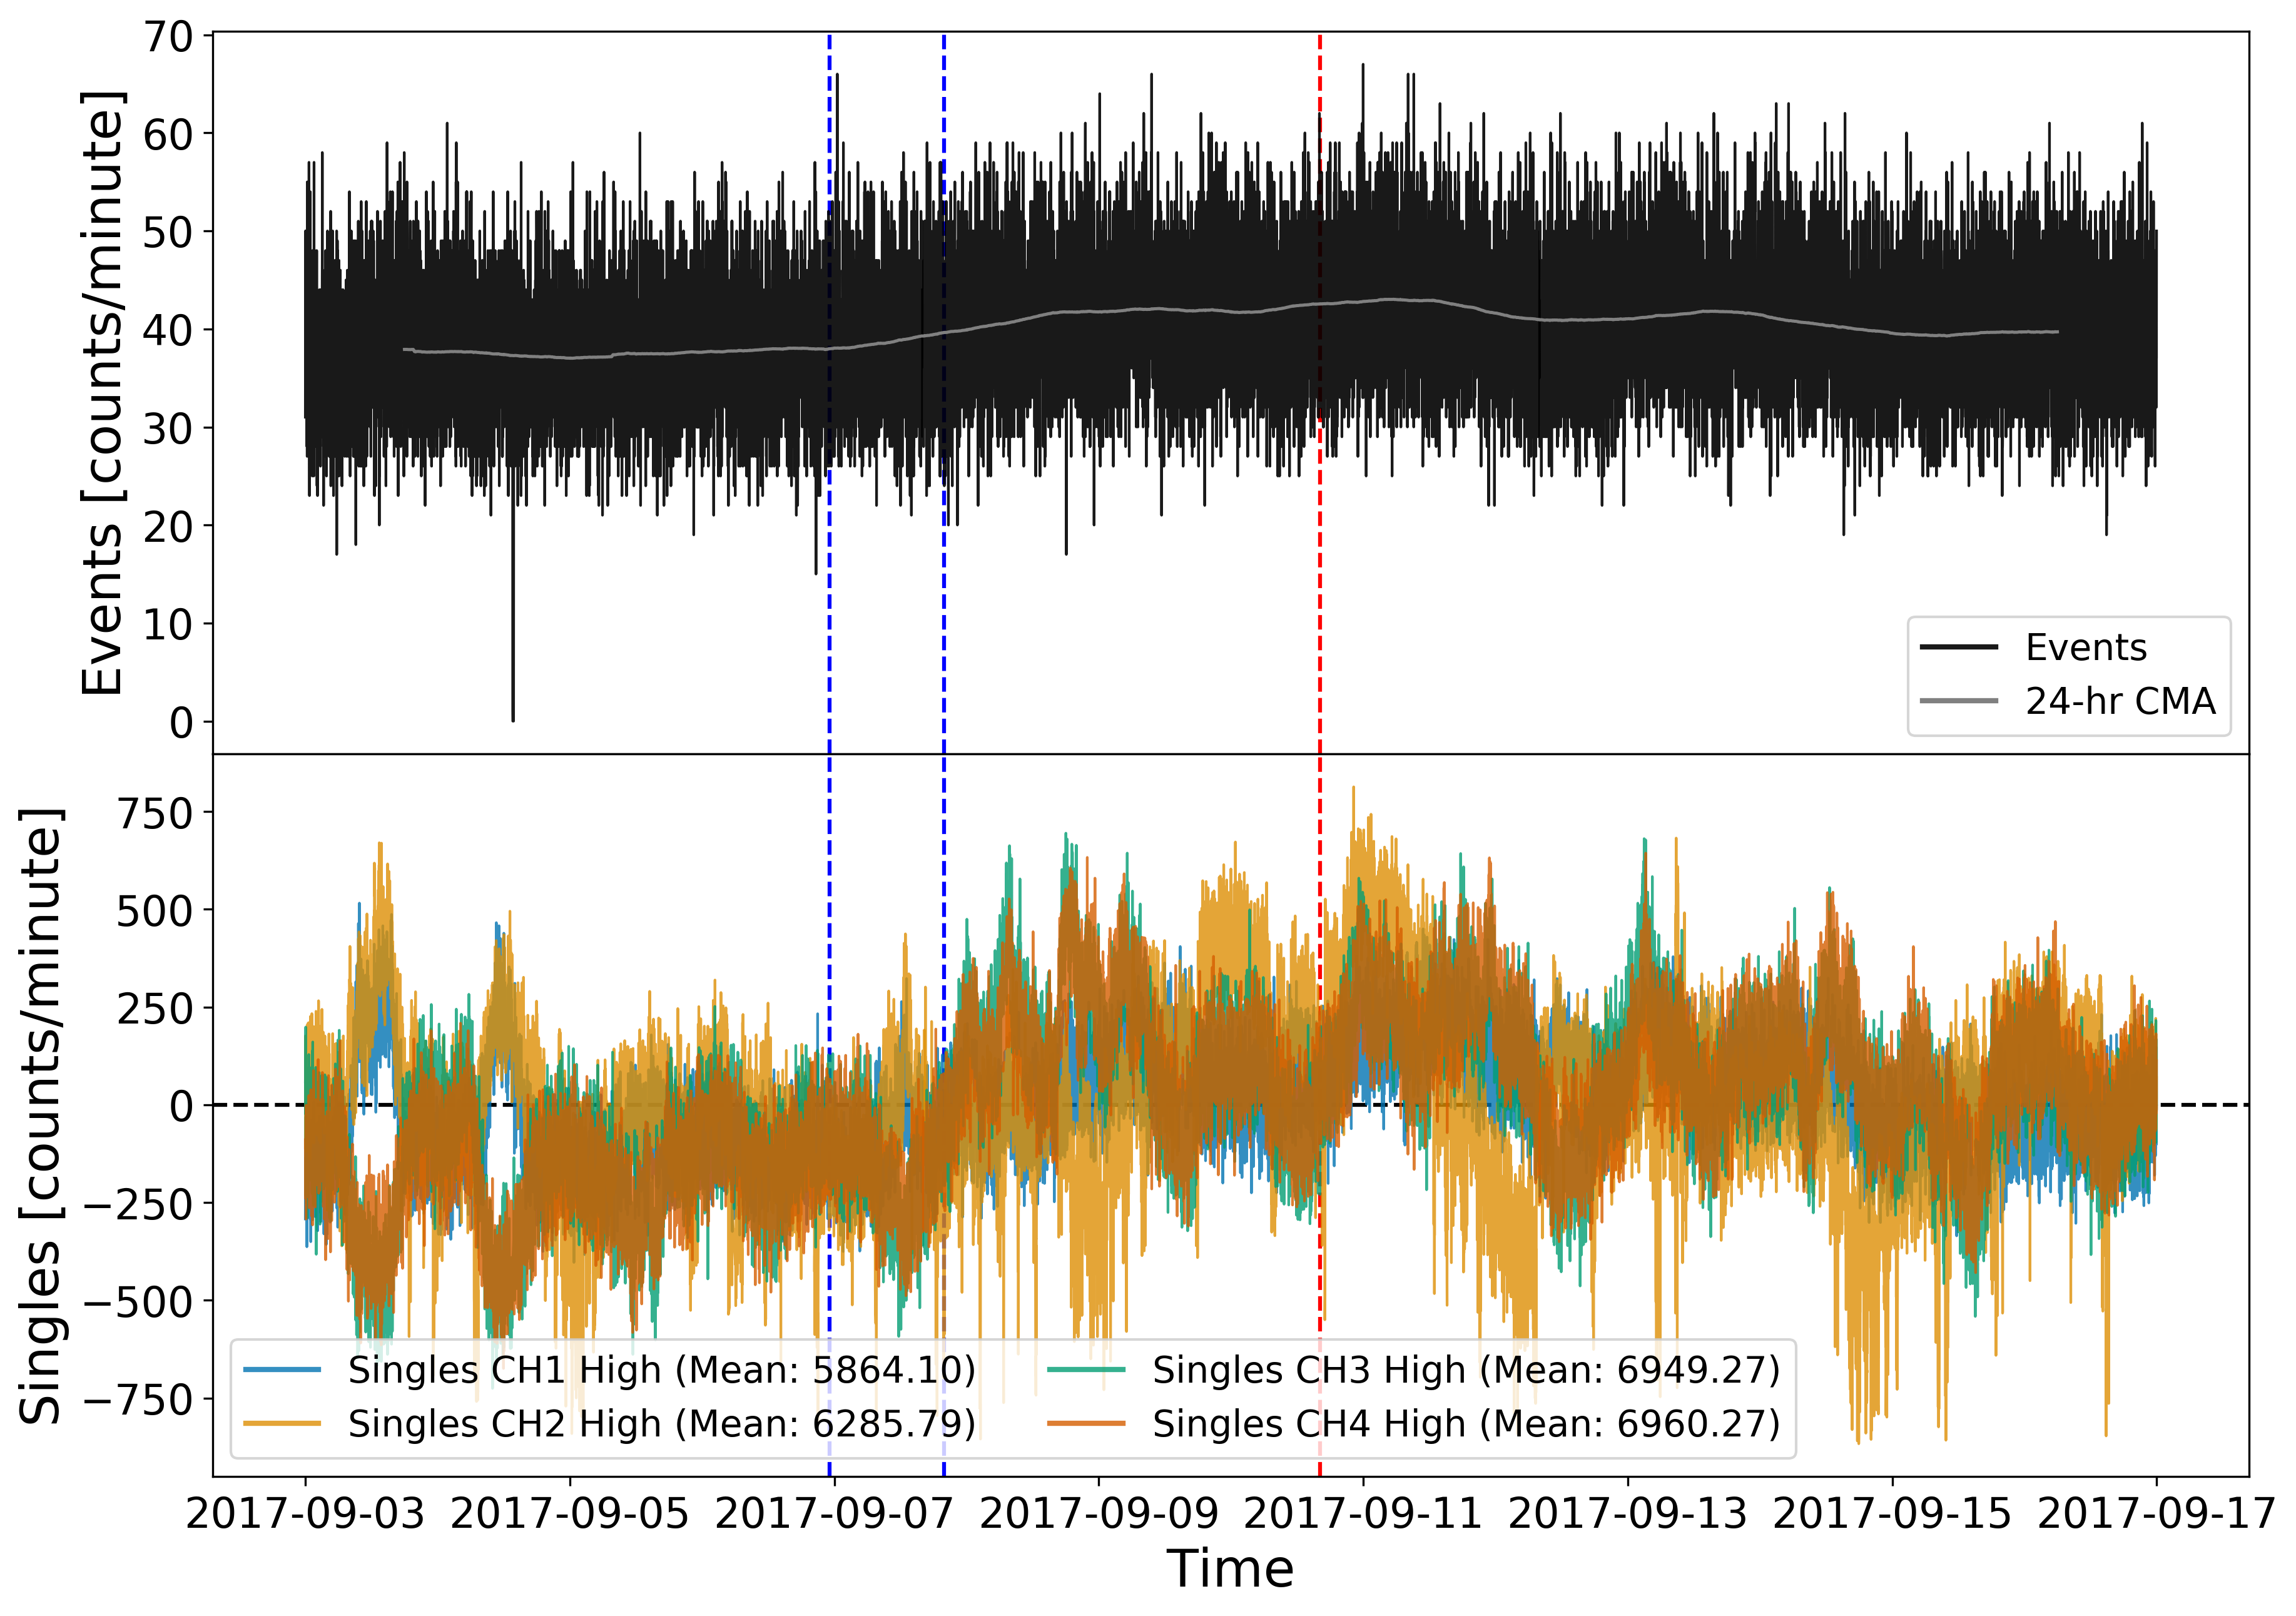
\includegraphics[width=0.48\columnwidth]{FD_GLE72_501.png}
		\label{fig:FD_GLE72_501}}
	%\qquad
	\subfloat[HS 203 (College Hageveld)]{
		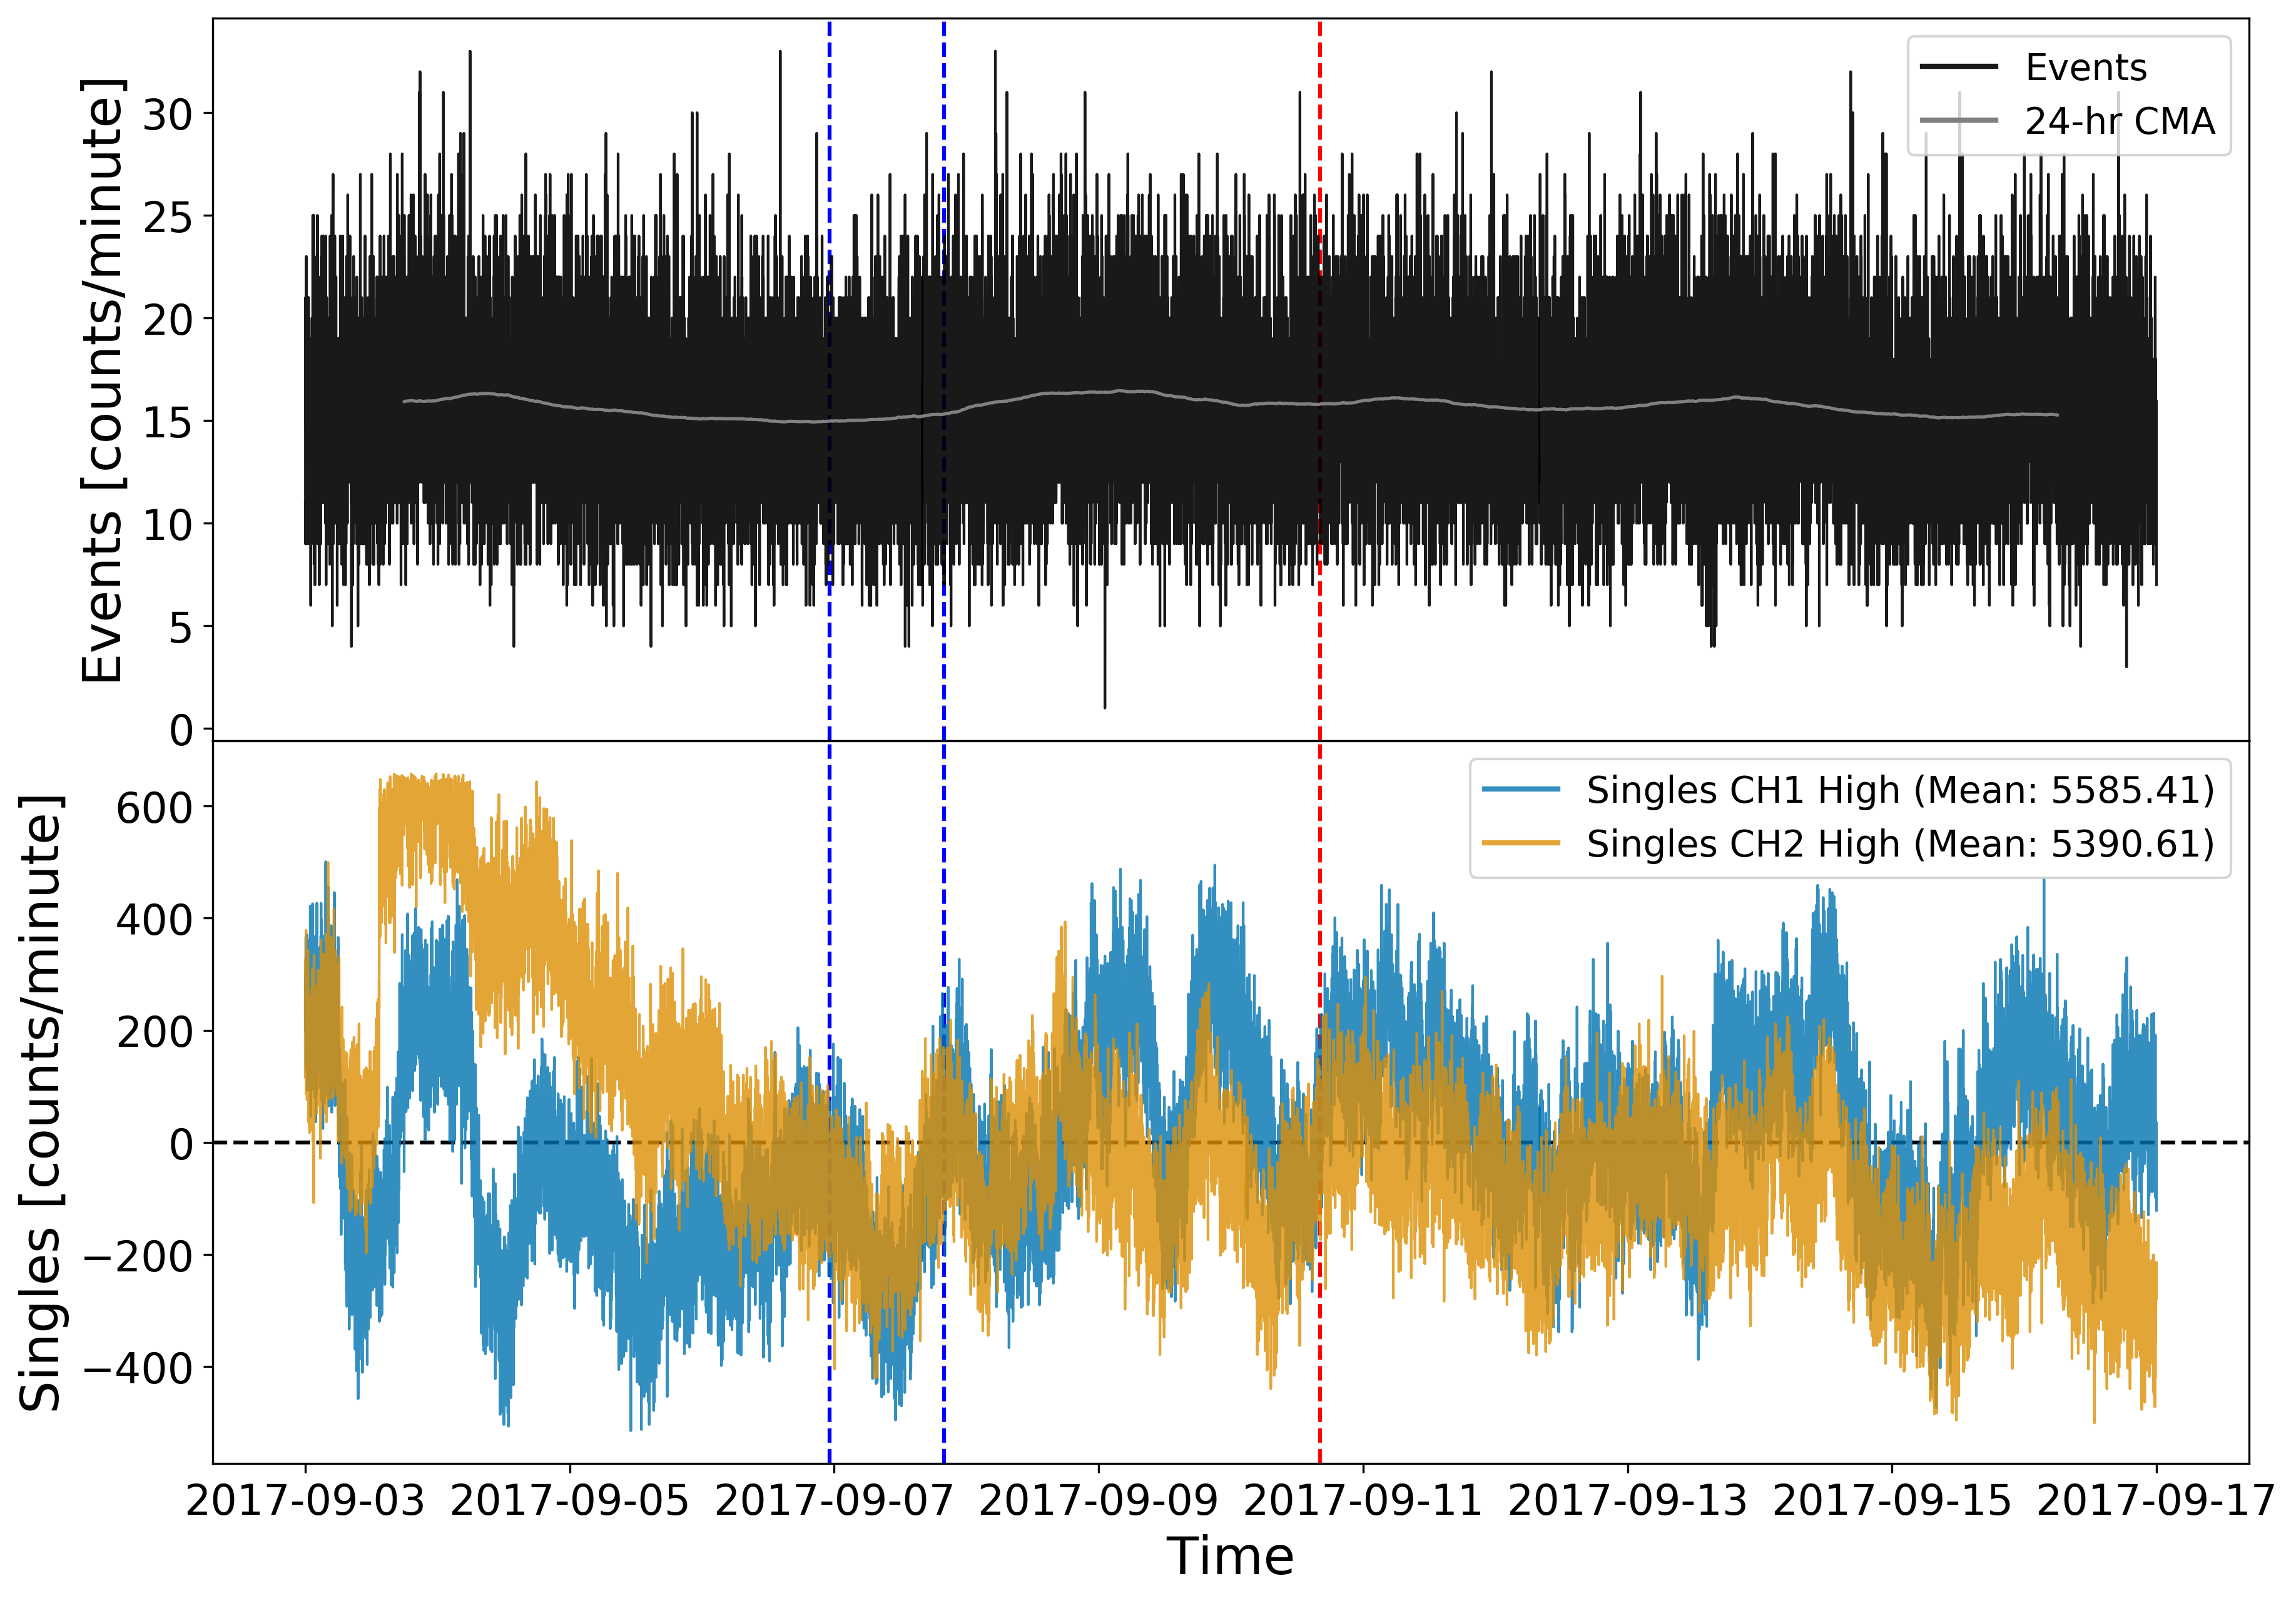
\includegraphics[width=0.48\columnwidth]{FD_GLE72_203.png}
		\label{fig:FD_GLE72_203}} \\
	
	\qquad
	
	\subfloat[HS 8001 (Eindhoven)]{
		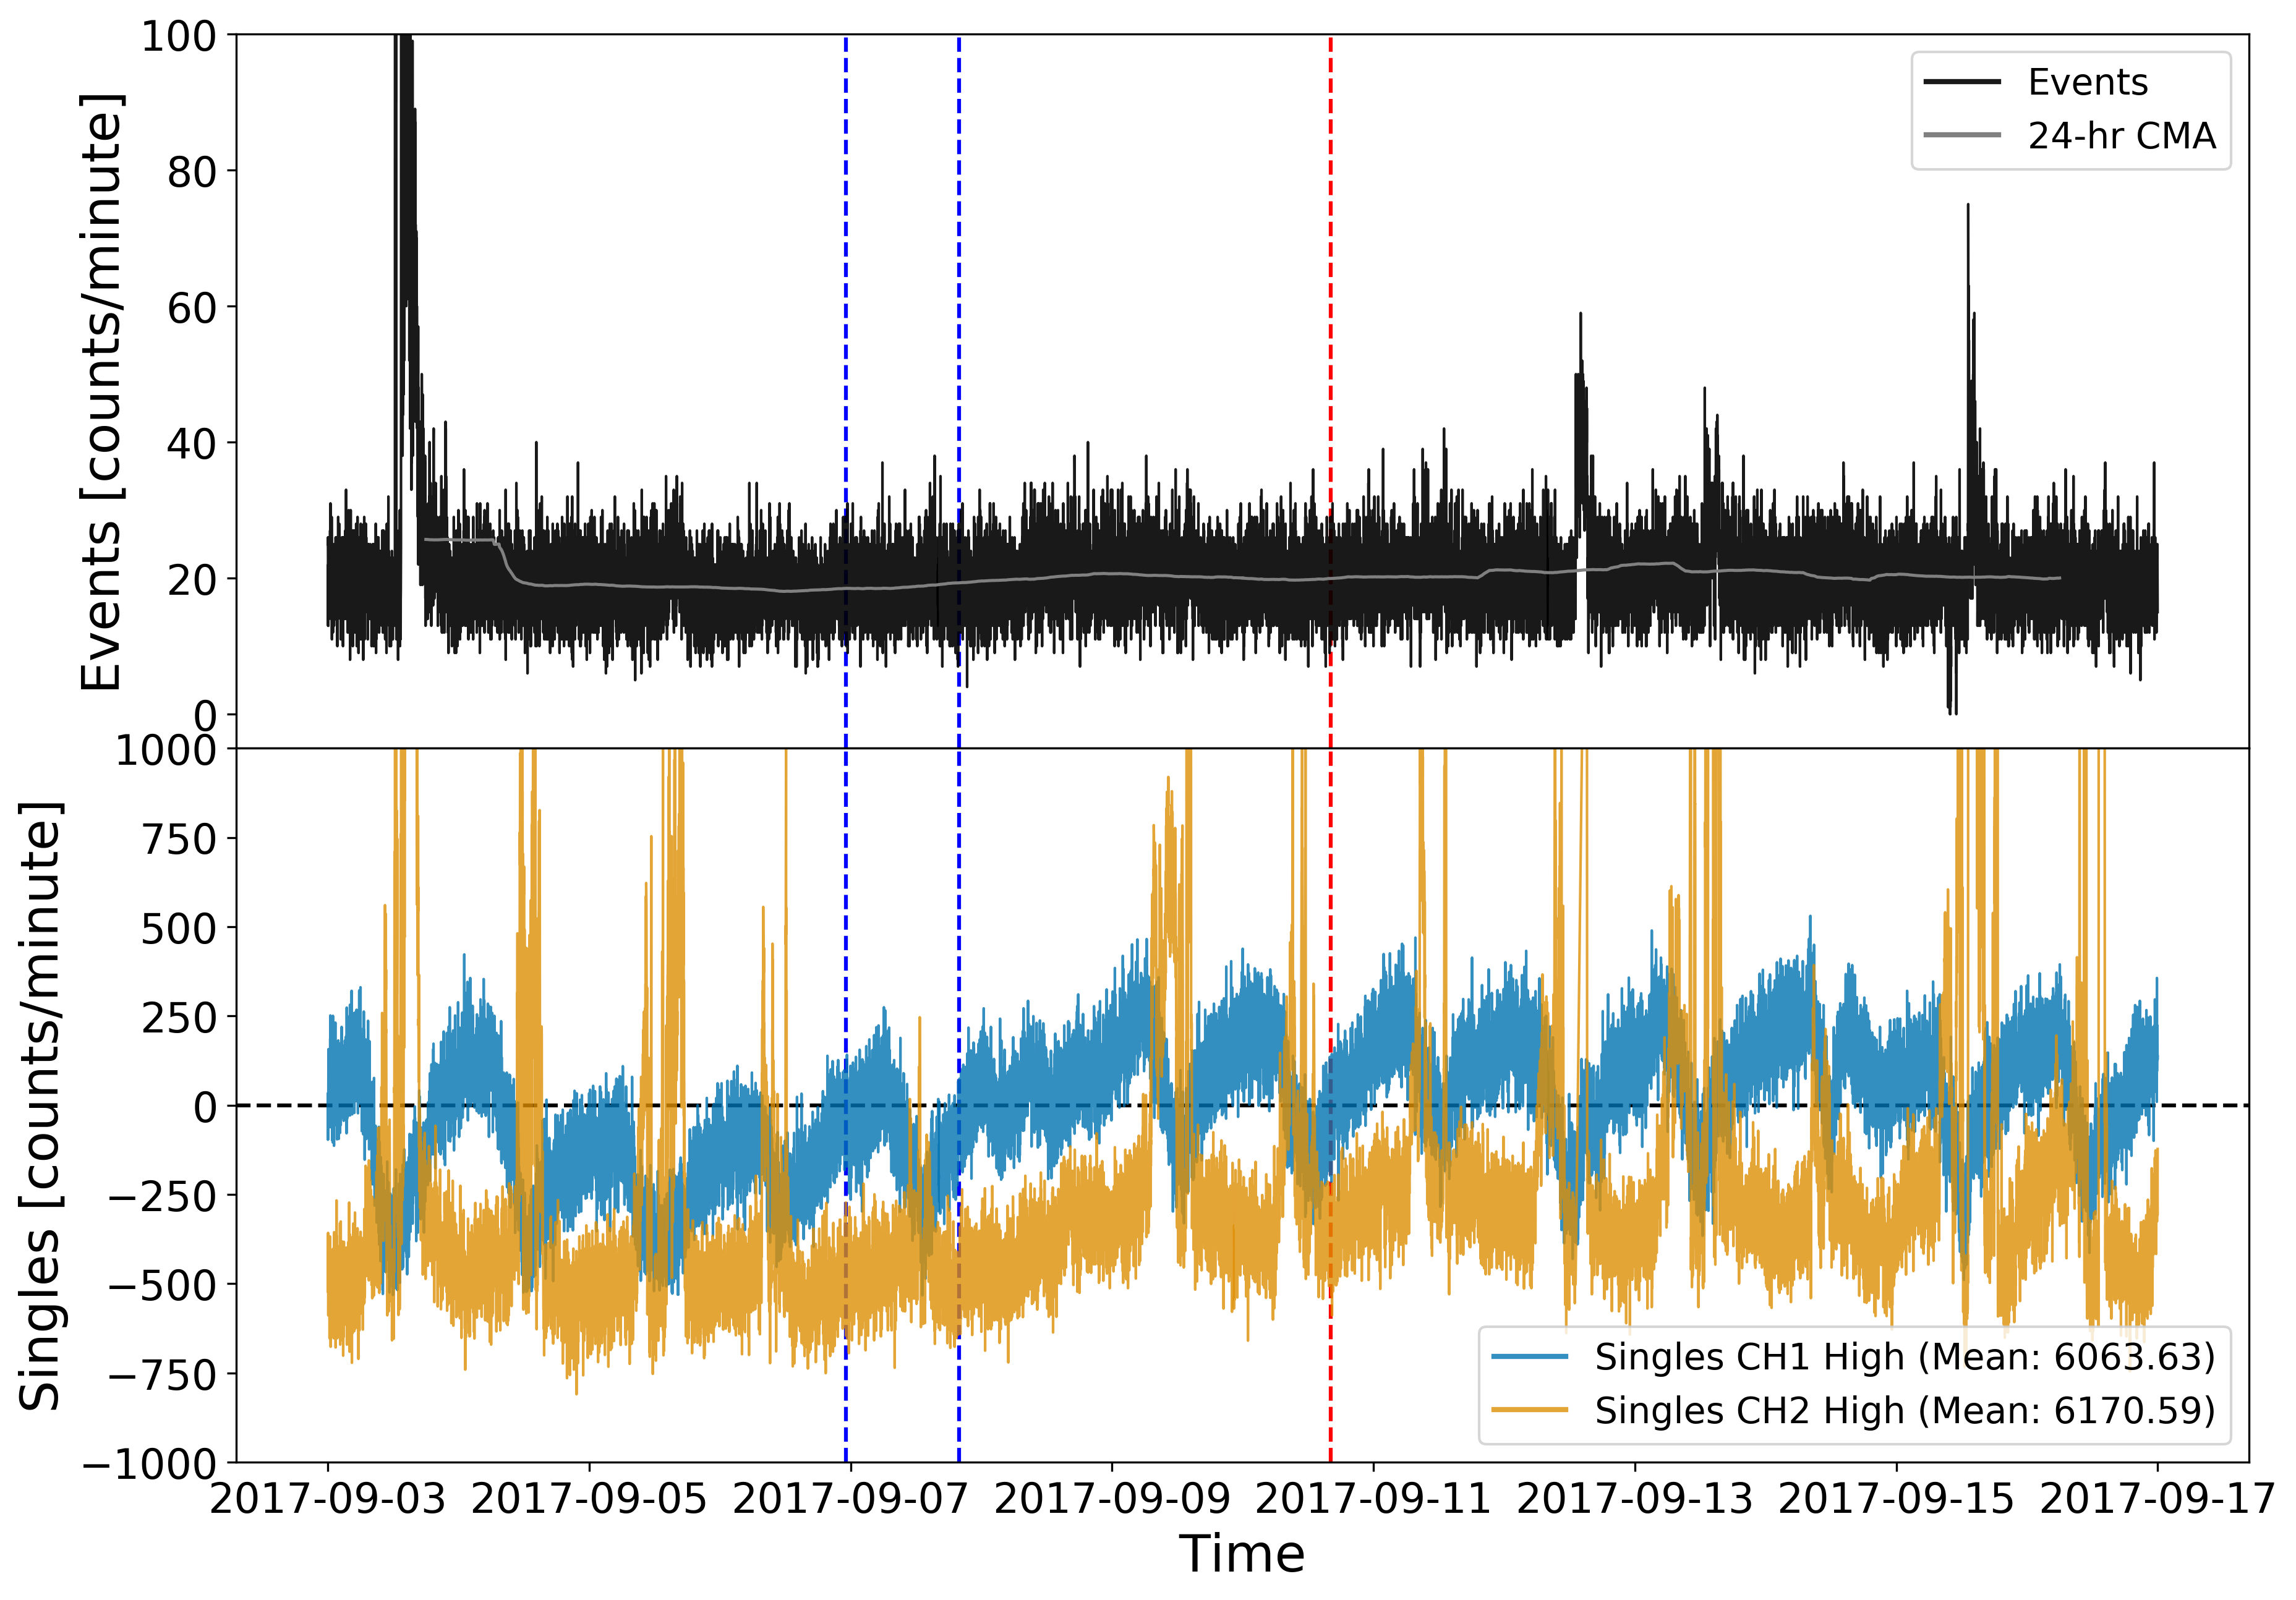
\includegraphics[width=0.48\columnwidth]{FD_GLE72_8001.png}
		\label{fig:FD_GLE72_8001}}
	%\qquad
	\subfloat[HS 14001 (Birmingham University)]{
		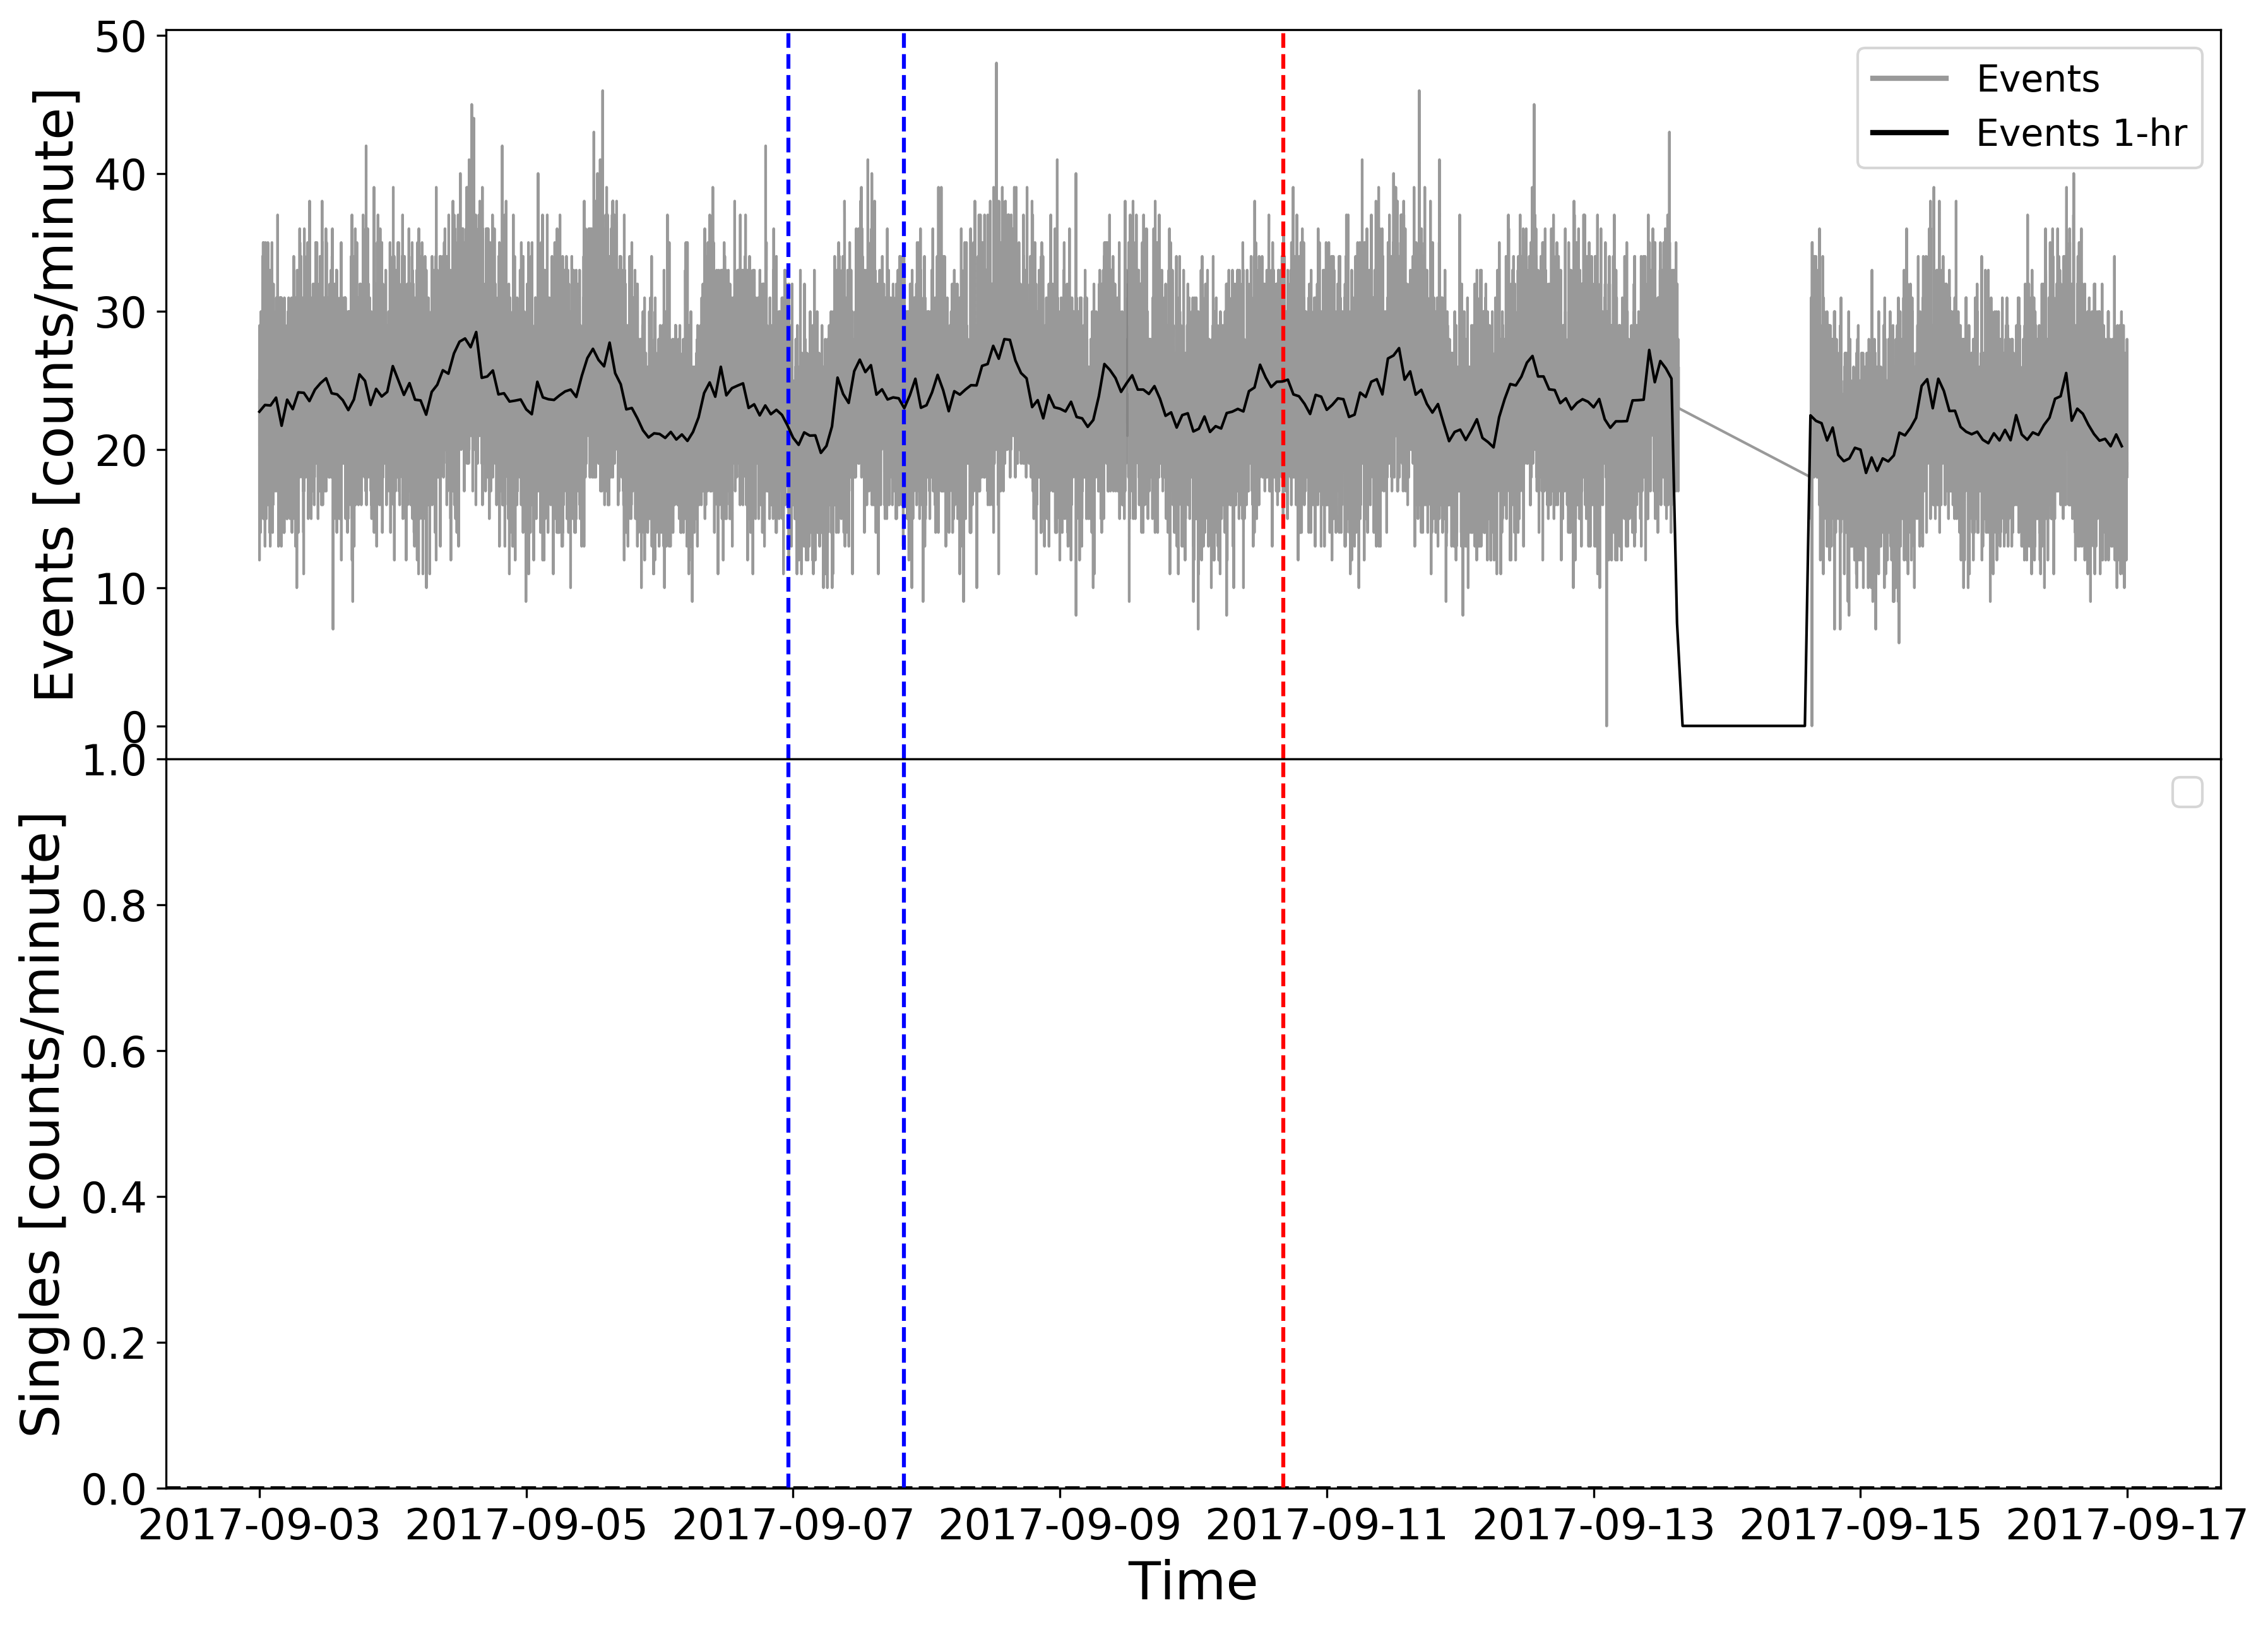
\includegraphics[width=0.48\columnwidth]{FD_GLE72_14001.png}
		\label{fig:FD_GLE72_14001}}
	
	\caption{HiSPARC data for [n] stations around the epoch in which there were several FDs close to the onset of GLE 72. The top panel of each subplot shows the minute-averaged trigger events between detectors within the station, while the bottom panel shows the mean-shifted, minute-averaged counts by each individual detector in the station. The vertical blue-dashed lines show the approximate onset-times of the two FDs observed around this epoch and the red-dashed line depicts the approximate onset time of the GLE.}
	\label{fig:FD_GLE72}
\end{figure}

... no clear FDs seen...



%%%%%%%%%%%%%%%%%%%%%%%%%%%%%%%%%%%%%%%%%%%%%%%%%%%%%%%%%%%%%%%%%%%%%
%%%%%%%%%%%%%%%%%%%%%%%%%%%%%%%%%%%%%%%%%%%%%%%%%%%%%%%%%%%%%%%%%%%%%
\section{Air Shower Simulations}\label{sec:CORSIKA}

In order to understand the footprint of air showers produced by PCRs, simulations of air showers were performed for a range of primary proton and $\alpha$-particle energies.

To simulate the CR air shower development, we employ CORSIKA ({\bf CO}smic {\bf R}ay {\bf SI}mulations for {\bf KA}scade), a Monte Carlo programme providing detailed simulations of the evolution of air showers initiated by cosmic rays particles through the atmosphere \citep{heck_extensive_2017}. The particles in the CORSIKA simulations are tracked through the atmosphere until they undergo interactions with atmospheric nuclei, decay due to their instability, or reach the ground level defined as the end of the simulation.

Proton and $\alpha$-particle initiated air showers were generated with energies ranging from $10^{9}$ to $10^{20}$~eV, and $4\times10^{9}$ to $10^{20}$~eV, respectively. In total $\sim 230000$ proton-initiated showers were simulated and $\sim 180000$ $\alpha$-particle-initiated air showers were simulated. The list of simulated air shower PCRs is shown in Table~\ref{tab:CORSIKA_sims}. For high energy, inelastic hadronic interactions within CORSIKA the QGSJET-II [REF] model was selected. Interactions of hadrons with energies below 80 GeV are simulated using GHEISHA [REF], which allowed for the simulation of PCRs in the regime of SCRs. In addition to these hadronic interactions, electromagnetic interactions within the CORSIKA simulations were described by the EGS4 [REF] model. Furthermore CORSIKA has a minimum muon energy limit that can be simulated of 10 MeV.

\begin{table}
	\begin{center}
	\caption{PCRs simulated using CORSIKA.}
	\label{tab:CORSIKA_sims}
	\begin{tabular}{l r l r | l r l r}
		\hline
		\multicolumn{4}{c}{\bf Protons}  & \multicolumn{4}{c}{\textbf{ $\bm{\alpha}$-Particles}}         \\
		    &    &    &    &    &    &    &    \\
		{\bf E$\bm{_{\mathrm{PCR}}}$ (eV)} & {\bf N$\bm{_{\mathrm{sims}}}$} & {\bf E$\bm{_{\mathrm{PCR}}}$ (eV)} & {\bf N$\bm{_{\mathrm{sims}}}$} & {\bf E$\bm{_{\mathrm{PCR}}}$ (eV)} & {\bf N$\bm{_{\mathrm{sims}}}$} & {\bf E$\bm{_{\mathrm{PCR}}}$ (eV)} & {\bf N$\bm{_{\mathrm{sims}}}$} \\
		\hline
		1.00E+09    & 10000   & 2.98E+12    & 1000    & 4.00E+09    & 10000   & 1.00E+13    & 1000    \\
		1.27E+09    & 10000   & 3.79E+12    & 1000    & 4.28E+09    & 10000   & 1.78E+13    & 100     \\
		1.62E+09    & 10000   & 4.83E+12    & 1000    & 5.46E+09    & 10000   & 3.16E+13    & 100     \\
		2.07E+09    & 10000   & 6.16E+12    & 1000    & 6.95E+09    & 10000   & 5.62E+13    & 100     \\
		2.64E+09    & 10000   & 7.85E+12    & 1000    & 8.86E+09    & 10000   & 1.00E+14    & 100     \\
		3.36E+09    & 10000   & 1.00E+13    & 1000    & 1.00E+10    & 10000   & 1.78E+14    & 50      \\
		4.28E+09    & 10000   & 1.78E+13    & 100     & 1.13E+10    & 10000   & 3.16E+14    & 50      \\
		5.46E+09    & 10000   & 3.16E+13    & 100     & 1.44E+10    & 10000   & 5.62E+14    & 50      \\
		6.95E+09    & 10000   & 5.62E+13    & 100     & 1.83E+10    & 10000   & 1.00E+15    & 10      \\
		8.86E+09    & 10000   & 1.00E+14    & 100     & 2.34E+10    & 10000   & 1.78E+15    & 10      \\
		1.00E+10    & 10000   & 1.78E+14    & 50      & 2.98E+10    & 10000   & 3.16E+15    & 10      \\
		1.13E+10    & 10000   & 3.16E+14    & 50      & 3.79E+10    & 10000   & 5.62E+15    & 10      \\
		1.44E+10    & 10000   & 5.62E+14    & 50      & 4.83E+10    & 10000   & 1.00E+16    & 10      \\
		1.83E+10    & 10000   & 1.00E+15    & 10      & 6.16E+10    & 10000   & 1.78E+16    & 10      \\
		2.34E+10    & 10000   & 1.78E+15    & 10      & 7.85E+10    & 10000   & 3.16E+16    & 10      \\
		2.98E+10    & 10000   & 3.16E+15    & 10      & 1.00E+11    & 10000   & 5.62E+16    & 10      \\
		3.79E+10    & 10000   & 5.62E+15    & 10      & 1.27E+11    & 1000    & 1.00E+17    & 10      \\
		4.83E+10    & 10000   & 1.00E+16    & 10      & 1.62E+11    & 1000    & 1.78E+17    & 10      \\
		6.16E+10    & 10000   & 1.78E+16    & 10      & 2.07E+11    & 1000    & 3.16E+17    & 10      \\
		7.85E+10    & 10000   & 3.16E+16    & 10      & 2.64E+11    & 1000    & 5.62E+17    & 10      \\
		1.00E+11    & 10000   & 5.62E+16    & 10      & 3.36E+11    & 1000    & 1.00E+18    & 10      \\
		1.27E+11    & 1000    & 1.00E+17    & 10      & 4.28E+11    & 1000    & 1.78E+18    & 10      \\
		1.62E+11    & 1000    & 1.78E+17    & 10      & 5.46E+11    & 1000    & 3.16E+18    & 10      \\
		2.07E+11    & 1000    & 3.16E+17    & 10      & 6.95E+11    & 1000    & 5.62E+18    & 10      \\
		2.64E+11    & 1000    & 5.62E+17    & 10      & 8.86E+11    & 1000    & 1.00E+19    & 10      \\
		3.36E+11    & 1000    & 1.00E+18    & 10      & 1.13E+12    & 1000    & 1.78E+19    & 10      \\
		4.28E+11    & 1000    & 1.78E+18    & 10      & 1.44E+12    & 1000    & 3.16E+19    & 10      \\
		5.46E+11    & 1000    & 3.16E+18    & 10      & 1.83E+12    & 1000    & 5.62E+19    & 10      \\
		6.95E+11    & 1000    & 5.62E+18    & 10      & 2.34E+12    & 1000    & 1.00E+20    & 10      \\
		8.86E+11    & 1000    & 1.00E+19    & 10      & 2.98E+12    & 1000    &             &         \\
		1.13E+12    & 1000    & 1.78E+19    & 10      & 3.79E+12    & 1000    &             &         \\
		1.44E+12    & 1000    & 3.16E+19    & 10      & 4.83E+12    & 1000    &             &         \\
		1.83E+12    & 1000    & 5.62E+19    & 10      & 6.16E+12    & 1000    &             &         \\
		2.34E+12    & 1000    & 1.00E+20    & 10      & 7.85E+12    & 1000    &             &         \\   
		\hline
	\end{tabular}
	\end{center}
\end{table}

There are several other user-definable setting within CORSIKA which are explained in-depth in the CORSIKA user's guide \citep{heck_extensive_2017}. The settings chosen within these simulation are breifly discussed below. Simulation thinning was enable in CORSIKA to reduce computation time and reduce the output file size. The observation level at which point the simulation cease was set at 100 m above sea level (compared to the $\sim 50$ m typical of the stations, however this difference is negligible for the air shower development.) The pre-defined central European atmosphere in October was used for all simulations, and western-European magnetic field was used as calculated with the \textit{Geomag} programme [REF]: B$_{\mathrm{x}}=18.799$~$\mu$T and B$_{\mathrm{z}}=44.980$~$\mu$T.


%%%%%%%%%%%%%%%%%%%%%%%%%%%%%%%%%%%%%%%%%%%%%%%%%%%%%%%%%%%%%%%%%%%%%
\subsection{Air Shower Footprints}\label{sec:CORSIKA_footprint}

The average footprint of muons at ground level was acquired from the output CORSIKA simulations. This was achieved by simply taking the distributino of the muons at ground level at the end of the simulation as a function of their distance from the shower core for each individual simulation realisation. For a given PCR energy the average air shower footprint distribution is calculated by combining the individual simulation realisations.

%[Discuss how distance between the HiSPARC station 2d/4d detectors will impact the ability to view certain PCR energies, and sets an lower limit on the energies observable in the standard trigger mode]

\begin{figure}
	\centering
	\subfloat[Proton initiated air shower. \label{fig:p_footprint}]{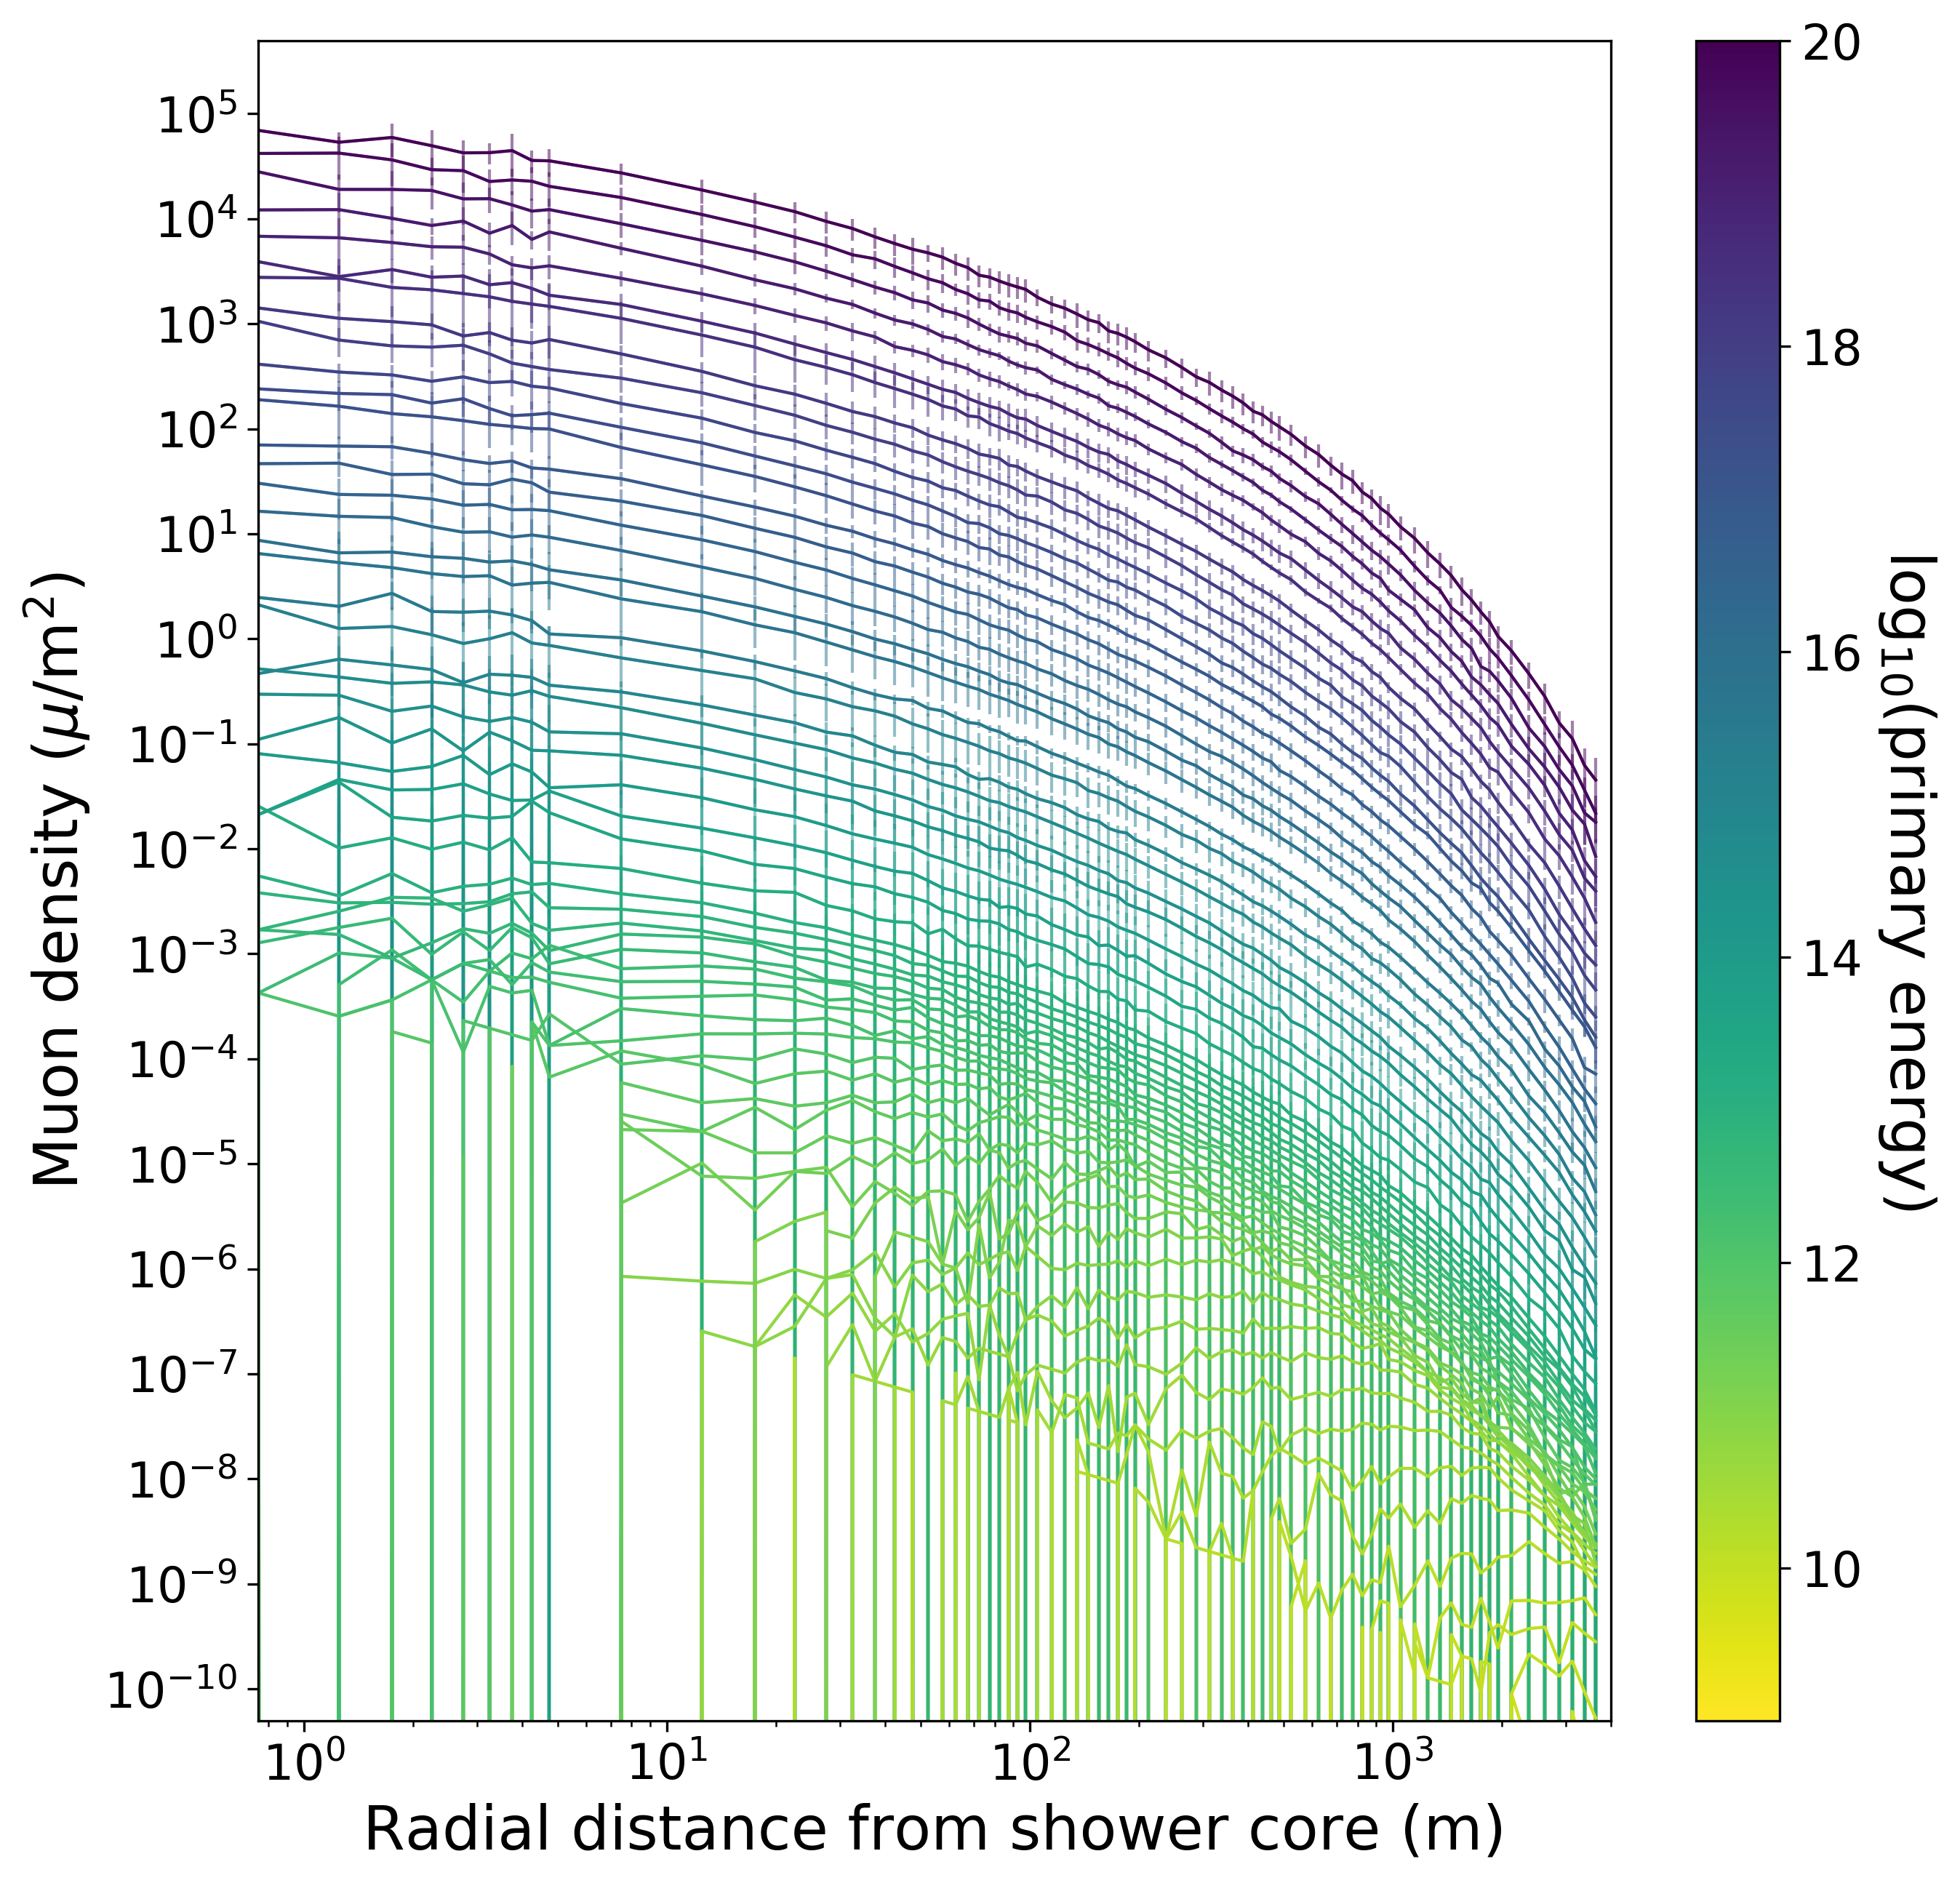
\includegraphics[width=0.47\columnwidth]{proton_footprint.png}} 
	\qquad
	\subfloat[$\alpha$-particle initiated air shower. \label{fig:a_footprint}]{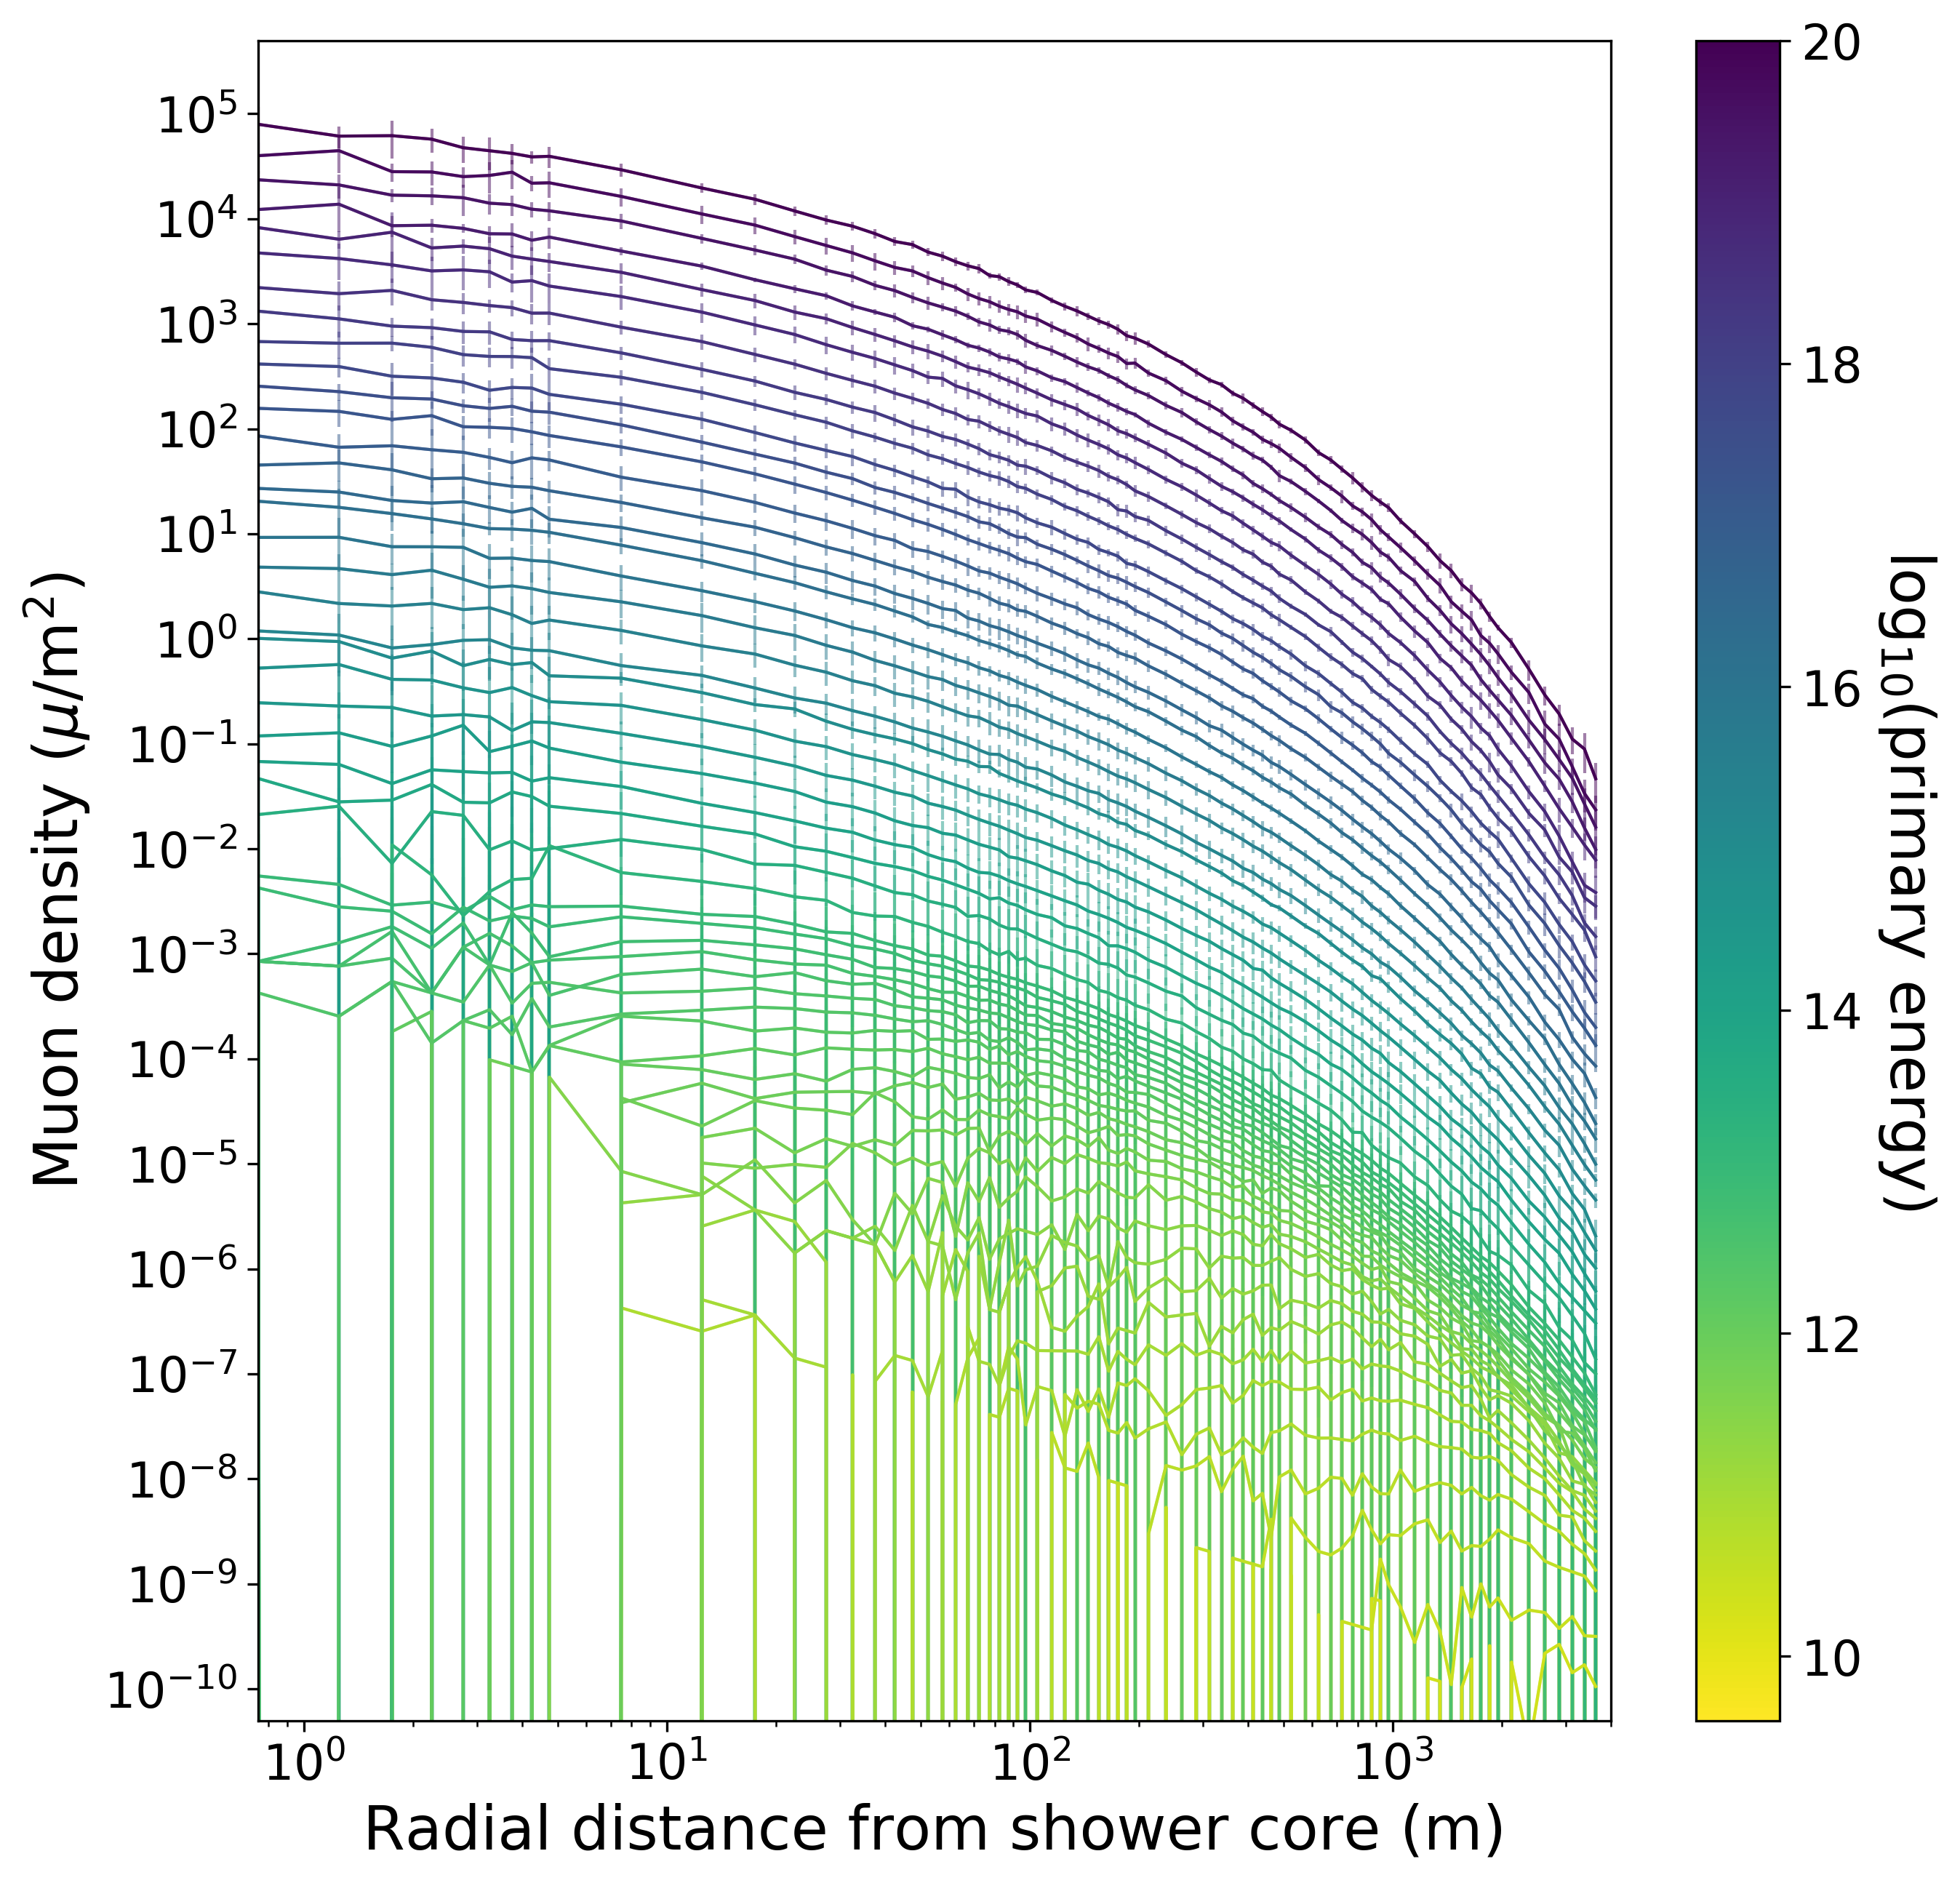
\includegraphics[width=0.47\columnwidth]{alpha_footprint.png}}
	\caption{Mean muon density footprints for (a) proton-initiated air showers and (b) $\alpha$-particle-initiated air showers with intial PCR trajectories with zenith angles $\theta=0^{\circ}$ and various PCR energies. The error bars given represent 1$\sigma$.} \label{fig:shower_footprints}
\end{figure}

The interpretation of Figure~\ref{fig:shower_footprints} can provide an understanding of the minimum energy of PCRs observable by the different stations within the HiSPARC network. The typical separation between the detectors in a HiSPARC station is $\sim 10$~m, however the separation between detectors can be up to as much as 20~m or as low as a couple of metres. This analysis of the air shower footprint shows the variation in PCR energy sampled varies marginally over this range of distances and suggests that HiSPARC stations will typical observe PCR with an energy of $\sim 10^{14}-10^{15}$~eV to meet the required trigger conditions.

%\begin{table}
%	\begin{center}
%		\caption{HS station minimum observable PCR energy}
%		\label{tab:footprints}
%		\begin{tabular}{l c c c}
%		\hline
%		{Station ID} & {Average separation (m)} & {Proton E$_{\mathrm{min}}$} & {$\alpha$-particle E$_{\mathrm{min}}$} \\
%		\hline
%		{501} & {11.2} & {} & {} \\
%		{14001} & {9.1} & {} & {} \\
%		{} & {} & {} & {} \\
%		\hline
%\end{tabular}
%\end{center}
%\end{table}


\subsection{Muon Flux}\label{sec:CORSIKA_flux}

From the air shower simulations it is possible to gain an estimate of the muon flux at groud-level based on the number of 

\begin{figure}
	\centering
	\subfloat[Proton initiated air shower. \label{fig:p_muons}]{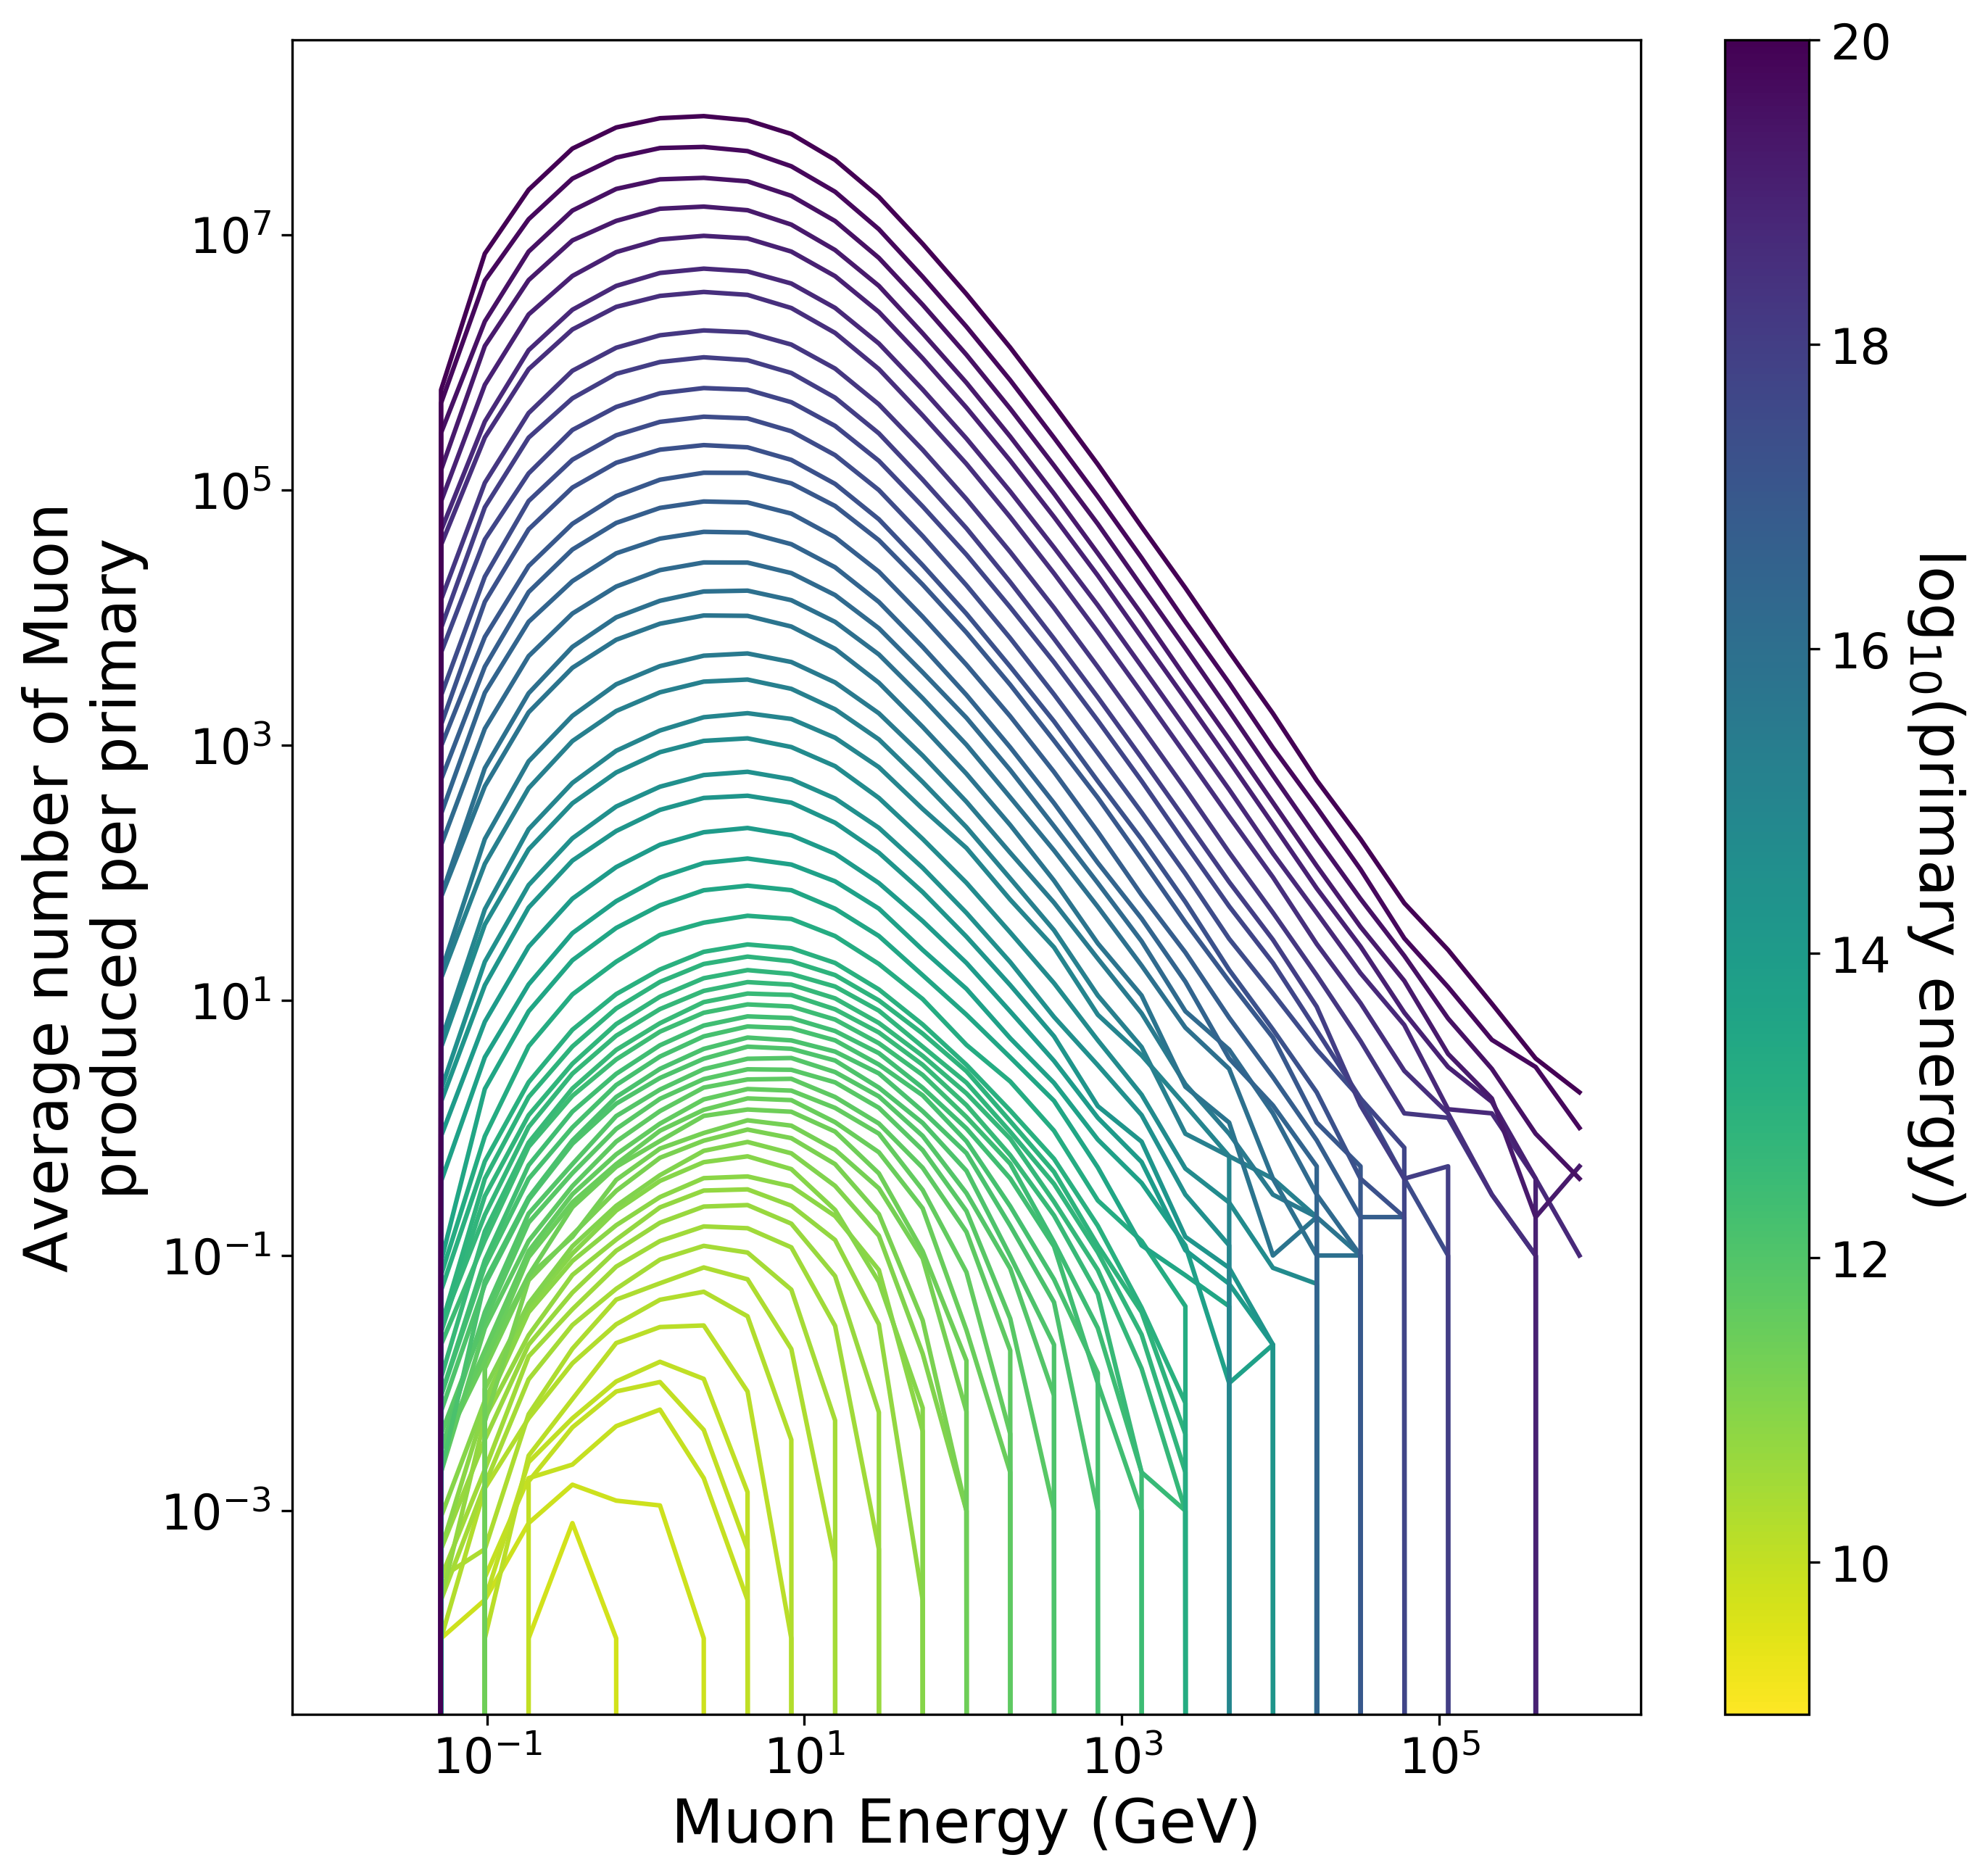
\includegraphics[width=0.47\columnwidth]{proton_muon_number.png}} 
	\qquad
	\subfloat[$\alpha$-particle initiated air shower. \label{fig:a_muons}]{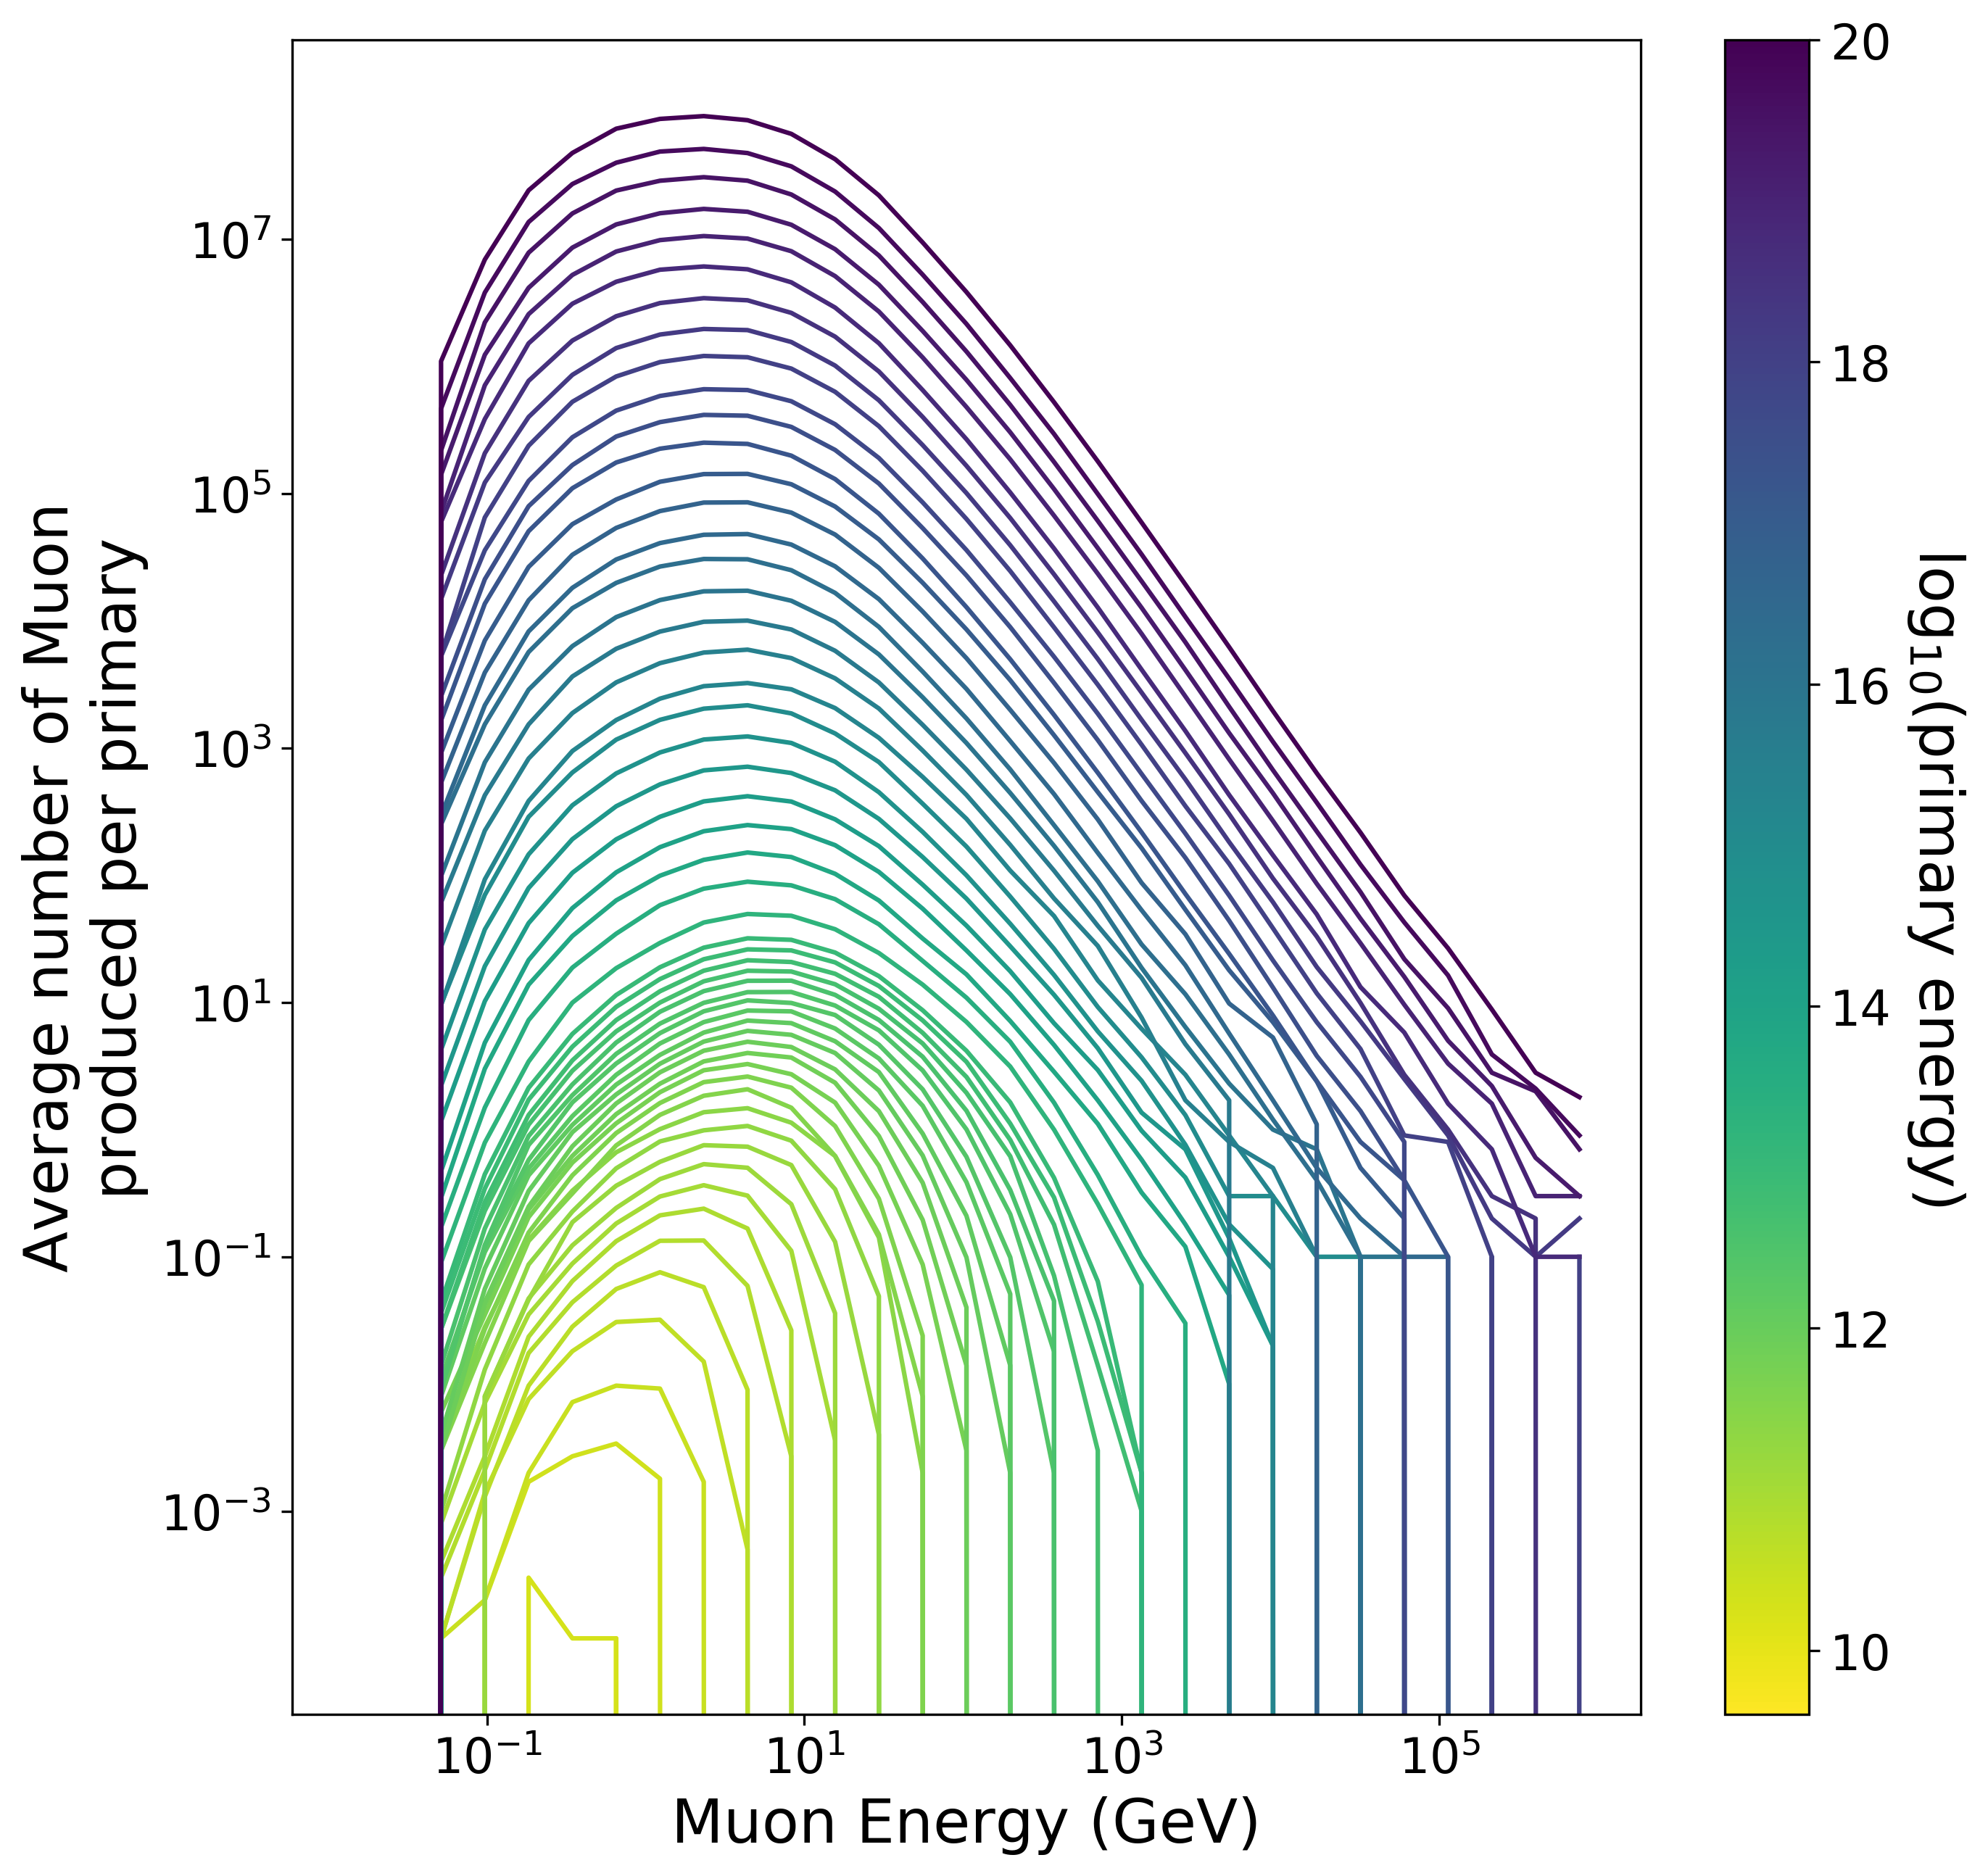
\includegraphics[width=0.47\columnwidth]{alpha_muon_number.png}}
	\caption{Mean number of muons produced at ground level by the PCR for (a) proton-initiated air showers and (b) $\alpha$-particle-initiated air showers, for various PCR energy. The uncertainty bars given represent 1$\sigma$.}
	\label{fig:shower_muons}
\end{figure}



%%%%%%%%%%%%%%%%%%%%%%%%%%%%%%%%%%%%%%%%%%%%%%%%%%%%%%%%%%%%%%%%%%%%%
%%%%%%%%%%%%%%%%%%%%%%%%%%%%%%%%%%%%%%%%%%%%%%%%%%%%%%%%%%%%%%%%%%%%%
\section{Standardisation of HiSPARC Data}\label{sec:HS_standardisation}

%%%%%%%%%%%%%%%%%%%%%%%%%%%%%%%%%%%%%%%%%%%%%%%%%%%%%%%%%%%%%%%%%%%%%
\subsection{Motivation}
- HiSPARC stations are individually managed and guidlines aren't stringent
- Variability between stations exists and also apparently between detectors within a station (i.e. see singles during GLE 72)

%%%%%%%%%%%%%%%%%%%%%%%%%%%%%%%%%%%%%%%%%%%%%%%%%%%%%%%%%%%%%%%%%%%%%
\subsection{Barometric Correction}\label{sec:HS_P_corr}

It is understood that observations made by ground-based CR detectors are susceptible to atmospheric conditions. Atmospheric pressure effects the CR travel path due to the expansion and contraction of the atmosphere with varying pressure; hence the CR counts are observed to be negatively correlated to atmospheric pressure as shown for both NMs and MDs in Figure~\ref{fig:CR_V_P}. A correction for this barometric effect is routinely applied as part of the data calibration for all NM stations within the NMDB NEST, but there is no such process in the HiSPARC network.


\begin{figure}[ht]
	\centering
	\subfloat[NM Station]{
		\includegraphics[width=0.48\columnwidth]{SOPO_CRvP.png}
		\label{fig:SOPO_CRvP}}
	%\qquad
	\subfloat[HS 501 (Nikhef)]{
		\includegraphics[width=0.48\columnwidth]{501_CRvP.png}
		\label{fig:HS_501_CRvP}} \\
	
	\caption{...}
	\label{fig:CR_V_P}
\end{figure}


The method of correcting for the barometric effect is discussed widely in the literature regarding NMs and is shown to depend on the barometric coefficient. Assuming the cosmic ray flux variation, absent of the atmospheric effects, is reaonably stable, then a simple corrected can be made. The CR variations ($N$) that depend on the local atmospheric pressure are described by equation~(\ref{eq:presscorr1}), where $\Delta N$ is the change in count rate, $\beta$ is the barometric coefficient, and $\Delta P = P - P_0$ is the deviation in pressure from the average ($P_0$) in the given time-period \citep{paschalis_online_2013}:

\begin{equation}
\Delta N = - \beta \, N \, \Delta P
\label{eq:presscorr1}
\end{equation}

Through the integration of equation~(\ref{eq:presscorr1}), the solution shows the dependence of cosmic ray intensity on pressure as given in equation~(\ref{eq:presscorr2}). 

\begin{equation}
N = N_{0} \, e^{-\beta \, \Delta P}
\label{eq:presscorr2}
\end{equation}

Therefore by taking the logarithm of equation~(\ref{eq:presscorr2}), one can obtain the barometric coefficient by fitting the straight line given by equation~(\ref{eq:presscorr3}) to the observed data, where $N_0$ may be assumed as the mean count rate over the given time-period of observations considered.

\begin{equation}
\mathrm{ln} \left( \frac{N}{N_0} \right) = - \beta \, \Delta P
\label{eq:presscorr3}
\end{equation}

A demonstration of the barometric correction method of fitting a straight line to the data described by equation~(\ref{eq:presscorr3}) is shown for both a NM and a HiSPARC station in Figure~\ref{fig:barometric_fit}.

\begin{figure}[ht]
	\centering
	\subfloat[SOPO NM Station]{
		\includegraphics[width=0.48\columnwidth]{SOPO_beta.png}
		\label{fig:SOPO_beta}}
	%\qquad
	\subfloat[HS 501 (Nikhef)]{
		\includegraphics[width=0.48\columnwidth]{501_beta.png}
		\label{fig:HS_501_beta}} \\
	
	\caption{The barometric coefficient calculation: (a) during November 2017 for the South Pole (SOPO) NM station, (b) during November 2019 for HiSPARC station 501 at Nikhef.}
	\label{fig:barometric_fit}
\end{figure}


An online barometric coefficient tool is available which allows user to perform the barometric correction for a given station over a user-defiend epoch (\url{http://cosray.phys.uoa.gr/index.php/data/nm-barometric-coefficient}). Using this tool, it was possible to provide a comparison between the method used in this work to that of the online NM barometric correction tool which is used for the correction of the NMDB stations. This is provided in Figure~\ref{fig:NM_beta_variation} for monthly corrections throughout 2017 for the NM station at the South Pole (SOPO).

\begin{figure}[ht]
	\centering
	\includegraphics[width=0.65\columnwidth]{SOPO_beta_2017.png}
	\caption{A comparison between the monthly barometric coefficient computed in this work and using the online barometric coefficient tool throughout the year 2017 for the SOPO NM station.}
	\label{fig:NM_beta_variation}
\end{figure}


Figure~\ref{fig:NM_beta_variation} shows a close agreement between the barometric coefficient calculated in this work and those acquired from the online tool for the SOPO NM. This was also true for other stations tested (APTY and ROME), thus providing confidence that the method used in this work was suitable for application on the HiSPARC data. The barometric correction was perfoemed on the stations where sufficient pressure data and count rates exist, and were re-investigated to determine whether the space weather events were observed in the HiSPARC data. These results are provided in Section \ref{sec:HS_obs_Pcorr}.



%%%%%%%%%%%%%%%%%%%%%%%%%%%%%%%%%%%%%%%%%%%%%%%%%%%%%%%%%%%%%%%%%%%%%
\subsection{Temperature Correction}\label{sec:HS_T_corr}

It has been discussed in the literature that the effect of atmospheric temperature on muon intensity has to be treated differently to the pressure effect \citep{berkova_temperature_2011}, as the temperature influences both the creation and disintegration processes for muons, such that there is a positive effect and a negative effect on muon intensity as a consequence of temperature variations \citep{mendoncca_temperature_2016}. 

The positive effect is related to pion decay and its dependence on temperature variation. The higher the temperature, the lower the atmospheric pion absorption, which implies a higher generation rate of muons \citep{mendoncca_temperature_2016}.

The negative effect corresponds to the decrease of muon intensity at ground level as the muon average path length varies with temperature. Due to the heating and the expansion of the atmosphere during summer periods muons are produced higher in the atmosphere; hence the muon propagation path increases meaning more atmosphere for muons to traverse before reaching the ground, and an increased decay probability and ionisation losses \citep{savic_pressure_2015, mendoncca_temperature_2016}.

Due to the difference in decay probability, the negative effects dominate for low energy muons (i.e. those detected by ground-level MDs), and the positive effect dominates for high energy muons (i.e. those detected by underground MDs) \citep{berkova_temperature_2011}; therefore it is expected that the negative effect should dominate for the HiSPARC network. Temperature effects are also observed by NMs; however the effect is less significant than for MDs hence temperature corrections are not widely applied for NMs \citep{mendoncca_temperature_2016}.

This is in contradiction with the observations of diurnal variation with the HiSPARC detector, as one can quite clearly see that the HiSPARC stations register higher count rates during local noon.

Several methods of correcting for the negative temperature effect are summarised by \cite{berkova_temperature_2011} which utilise different measures of atmospheric temperature when performing the temperature correction. \cite{mendoncca_temperature_2016} provides a comparative summary of these methods applied to correct for atmospheric temperature variations observed by GMDN detectors. The methods discussed here however are typically applied over long timescales of years with low temporal resolution rather than to account for short timescale variations with periods of less than a day; hence the suitability of these methods is uncertain.

\cite{mendoncca_temperature_2016} concludes that correcting for temperature using the atmospheric mass weighted temperature is one of the most suitable methods for the GMDN as it allows for the highest correlation between long-term CR variations and temperature. The mass weighted method is an approximation for integrating over the vertical atmospheric temperature as is given in Eq. (\ref{eq:tempcorr}):

\begin{equation}
\left( \frac{\Delta N}{N} \right)_T = \, \bar{\alpha}  \int^{h_0}_{0}  \, \delta \, T(h) \, dh = \sum_{i=0}^{n} \frac{x(h_i) - x(h_{i+1})}{x(h_0)} T(h_i)  = \alpha_{\mathrm{MSS}} \delta T_{\mathrm{MSS}}
\label{eq:tempcorr}
\end{equation}

where $h_0$ is the closest to ground altitude; $\delta T_{\mathrm{MSS}}$ is the deviation of the mass weighted atmospheric temperature; $T(h_i)$ is the temperature in degrees kelvin observed at the altitude $h_i$; $x(h_ i)$ is the atmospheric depth at the altitude $h_i$ which is given by Eq. \ref{eq:atmos_depth}:

\begin{equation}
x(h) = \int^{\infty}_{h}  \, \rho (h) \, dh  \, \rho (h) = \frac{P(h)}{T(h)} \frac{M_{mol}}{R} 
\label{eq:atmos_depth}
\end{equation}

where $P(h)$ is the atmospheric pressure profile as a function of depth; $T(h)$ is the atmospheric temperature; $\rho(h)$ is the air density at a given altitude $h$; $M_{mol}$ is the molar mass of air; $R$ is the universal gas constant.

The temperature correction is therefore used in a formalism the same as Eq. (\ref{eq:presscorr3}), replacing replacing $\beta$ for $\alpha$ and $\Delta P$ for $\Delta T$.

In addition it is discussed by \cite{berkova_temperature_2011} and \cite{mendoncca_temperature_2016} that the effective generation level temperature is a suitable assumption for this purpose. This method is based on the assumption that muons are mostly generated at a certain isobaric level, taken as 100 mbar, and therefore the temperature at 100 mbar in the atmospheric pressure profile is used, $T_{\mathrm{100 \, mbar}}$.

As discussed above, \cite{mendoncca_temperature_2016} provide this as a method for correcting for the long-term variation in atmospheric temperature which varies seasonally rather than to correct for diurnal variations; therefore it is unsure how relevant this method of atmospheric temperature correction will be to the diurnal variations observed in the HiSPARC data.



 

%%%%%%%%%%%%%%%%%%%%%%%%%%%%%%%%%%%%%%%%%%%%%%%%%%%%%%%%%%%%%%%%%%%%%
%%%%%%%%%%%%%%%%%%%%%%%%%%%%%%%%%%%%%%%%%%%%%%%%%%%%%%%%%%%%%%%%%%%%%
\section{HiSPARC Observations After Pressure Corrections}\label{sec:HS_obs_Pcorr}


%%%%%%%%%%%%%%%%%%%%%%%%%%%%%%%%%%%%%%%%%%%%%%%%%%%%%%%%%%%%%%%%%%%%%
\subsection{Pressure Corrected Observations of Ground Level Enhancements}


\begin{figure}[ht]
	\centering
	\subfloat[...]{
		\includegraphics[width=0.48\columnwidth]{GLE71_3001_Pcorr.png}
		\label{fig:GLE71_3001_Pcorr}}
	%\qquad
	\subfloat[...]{
		\includegraphics[width=0.48\columnwidth]{GLE71_8001_Pcorr.png}
		\label{fig:GLE71_8001_Pcorr}} \\
	
	
	\caption{Pressure corrected HiSPARC data for 2 stations around the epoch of GLE 71. The top panel of each subplot shows the minute-averaged trigger events between detectors within the station, while the bottom panel shows the mean-shifted, minute-averaged counts by each individual detector in the station. The vertical red, dashed line depicts the approximate onset time of the GLE.}
	\label{fig:GLE_71_Pcorr}
\end{figure}


\begin{figure}[ht]
	\centering
	\subfloat[HS 501 (Nikhef)]{
		\includegraphics[width=0.48\columnwidth]{GLE72_501_Pcorr.png}
		\label{fig:GLE72_501_Pcorr}}
	%\qquad
	\subfloat[HS 203 (College Hageveld)]{
		\includegraphics[width=0.48\columnwidth]{GLE72_203_Pcorr.png}
		\label{fig:GLE72_203_Pcorr}} \\
	
	
	\caption{Pressure corrected HiSPARC data for 2 stations around the epoch of GLE 72. The top panel of each subplot shows the minute-averaged trigger events between detectors within the station, while the bottom panel shows the mean-shifted, minute-averaged counts by each individual detector in the station. The vertical red, dashed line depicts the approximate onset time of the GLE.}
	\label{fig:GLE_72_Pcorr}
\end{figure}


%%%%%%%%%%%%%%%%%%%%%%%%%%%%%%%%%%%%%%%%%%%%%%%%%%%%%%%%%%%%%%%%%%%%%
\subsection{Pressure Corrected Observations of Forbush Decreases}



\begin{figure}[ht]
	\centering
	\includegraphics[width=0.65\columnwidth]{FD_201207_8001_Pcorr.png}
	\caption{...}
	\label{fig:FD_201207_8001_Pcorr}
\end{figure}



\begin{figure}[ht]
	\centering
	\includegraphics[width=0.65\columnwidth]{FD_201412_501_Pcorr.png}
	\caption{...}
	\label{fig:FD_201412_501_Pcorr}
\end{figure}



\begin{figure}[ht]
	\centering
	\subfloat[HS 501 (Nikhef)]{
		\includegraphics[width=0.48\columnwidth]{FD_GLE72_501_Pcorr.png}
		\label{fig:FD_GLE72_501_Pcorr}}
	%\qquad
	\subfloat[HS 203 (College Hageveld)]{
		\includegraphics[width=0.48\columnwidth]{FD_GLE72_203_Pcorr.png}
		\label{fig:FD_GLE72_203_Pcorr}} \\
	
	
	\caption{Pressure corrected HiSPARC data for [n] stations around the epoch in which there were several FDs close to the onset of GLE 72. The top panel of each subplot shows the minute-averaged trigger events between detectors within the station, while the bottom panel shows the mean-shifted, minute-averaged counts by each individual detector in the station. The vertical blue-dashed lines show the approximate onset-times of the two FDs observed around this epoch and the red-dashed line depicts the approximate onset time of the GLE.}
	\label{fig:FD_GLE72_Pcorr}
\end{figure}



%%%%%%%%%%%%%%%%%%%%%%%%%%%%%%%%%%%%%%%%%%%%%%%%%%%%%%%%%%%%%%%%%%%%%
%%%%%%%%%%%%%%%%%%%%%%%%%%%%%%%%%%%%%%%%%%%%%%%%%%%%%%%%%%%%%%%%%%%%%
\section{Discussion}\label{sec:HS_discussion}

Throughout this chapter the feasibility of using the HiSPARC network of muon detectors has been analysed. This has involved performing cosmic ray air shower simluations using CORSIKA and performing backwards

%HiSPARC 14008
\chapter{HiSPARC Station 14008}\label{chap:HiSPARC_14008}

%%%%%%%%%%%%%%%%%%%%%%%%%%%%%%%%%%%%%%%%%%%%%%%%%%%%%%%%%%%%%%%%%%%%%
%%%%%%%%%%%%%%%%%%%%%%%%%%%%%%%%%%%%%%%%%%%%%%%%%%%%%%%%%%%%%%%%%%%%%
\section{Introduction}\label{sec:HS_14008_intro}


%... [on daily variations (DV)] Dr. Rolf Butikofer (in a reply from Danislav Sapundjiev, dasapund@meteo.be) said:
%
%\textit{"The daily cosmic ray variation near Earth is caused by the anisotropy of the cosmic ray intensity in the interplanetary space. Cosmic ray particles follow the field lines of the interplanetary magnetic field when they travel towards the interior of the heliosphere. Because of the rotation of the Earth, the angle between the asymptotic cone of acceptance of various energies at the location of ground-based cosmic ray detectors (neutron monitors) and the direction of the interplanetary magnetic field varies with a time period of 24 hours. As a consequence cosmic ray detectors look in different directions in the course of a day and observe therefore a diurnal variation. The daily variations of neutron monitors is mainly seen by high latitude stations which have asymptotic directions at low energies (rigidities) near the equator."}



It was shown in Chapter~\ref{chap:HiSPARC}, using data acquired by the \gls{hisparc} network, that in its original configuration, \gls{hisparc} was not adequate for observing space weather events. In part, we showed that this was due to the low-magnitude of the increase in the expected muon flux during such events. Also relevant was the current configuration's bias towards higher energy \glspl{cr} and the sensitivity of the detectors to variations in meteorological conditions.

To some extent, it was possible to eliminate the variation in \glspl{cr} due to meteorological variations in the \gls{hisparc} data; however, it was shown to not always be effective, as different detectors in the \gls{hisparc} network displayed different responses to pressure and temperature variation and the correlation between atmospheric temperature and \gls{cr} count was weaker than the counterpart for pressure.

Thermal fluctuations in the atmosphere induce thermal noise in the \glspl{pmt} and although the temperature inside the \gls{hisparc} roof boxes has not been measured, it is suspected that the \glspl{pmt} can get quite hot, in particular when the roof boxes are in direct sunlight. We reported in Chapter~\ref{chap:HiSPARC} that the singles data represented our best possibility of observing lower-energy \glspl{pcr}; however, these data are most susceptible to the induced thermal noise as the temperature of the \gls{pmt} changes. Without measuring this temperature directly, a complete correction of this effect in the existing \gls{hisparc} data was not possible.

In this chapter we describe an alternative configuration of \gls{hisparc} station, which was devised and tested, to minimise these limiting effects. An instance of thermal noise in a single \gls{pmt} will be random, and uncorrelated with an instance of thermal noise in another \gls{pmt}. To exploit this, we stacked two detectors on top of each other and put them in coincidence to measure a single muon which traverses both scintillators, hence inducing signals in both \glspl{pmt}.




%%%%%%%%%%%%%%%%%%%%%%%%%%%%%%%%%%%%%%%%%%%%%%%%%%%%%%%%%%%%%%%%%%%%%
%%%%%%%%%%%%%%%%%%%%%%%%%%%%%%%%%%%%%%%%%%%%%%%%%%%%%%%%%%%%%%%%%%%%%
\section{Aims}\label{sec:HS_14008_aims}

The principal aim of building a new \gls{hisparc} station was to investigate whether an alternative configuration of a \gls{hisparc} station could minimise atmospheric variations in the data. In addition, we aimed to demonstrate a configuration that allowed for the observation of space weather events.

We aimed to set up a new detector, perform the relevant atmospheric corrections, where necessary, and review the noise properties of the detector. Furthermore, we also aimed to perform simulations of \glspl{gle} of varying physical properties to understand what magnitude of \gls{gle} could be observed with the new set-up. This would help us to understand how likely it was to observe the any space weather events with the alternative \gls{hisparc} station configuration.



%%%%%%%%%%%%%%%%%%%%%%%%%%%%%%%%%%%%%%%%%%%%%%%%%%%%%%%%%%%%%%%%%%%%%
%%%%%%%%%%%%%%%%%%%%%%%%%%%%%%%%%%%%%%%%%%%%%%%%%%%%%%%%%%%%%%%%%%%%%
\section{HiSPARC Station 14008 Set-up}\label{sec:HiSPARC_14008}


%%%%%%%%%%%%%%%%%%%%%%%%%%%%%%%%%%%%%%%%%%%%%%%%%%%%%%%%%%%%%%%%%%%%%
\subsection{Configuration}

The new configuration, of \gls{hisparc} station 14008, is shown in Figure~\ref{fig:14008_config}; it is composed of two detectors stacked on top of each other, both inside one roof box, and the signals from the \glspl{pmt} are put in coincidence. This configuration is advantageous over the single-scintillator, single-\gls{pmt} \gls{hisparc} set-up, as it allows the measurement of single muons that traverse both scintillators. 


\begin{figure}[ht!]
	\center
	\includegraphics[width=0.75\columnwidth]{14008_config.png}
	\caption{Schematic diagram of the HiSPARC station 14008 detector set-up within the roof box.}
	\label{fig:14008_config}
\end{figure}

We showed in Chapter~\ref{chap:HiSPARC} that the existing \gls{hisparc} design, requiring coincident triggers between detectors spaced tens of metres apart, biased the observations to higher \gls{pcr} energies and single muons from lower energy \glspl{pcr} could not be counted. Previously, we could only count single muons in the singles rates, but we have shown that the data were inconsistent between stations and it was difficult to disentangle the effects of temperature, \gls{pmt} noise, and the diurnal effect in the data. This stacked-configuration design reduces the energy bias in the events data, as it no longer requires the large footprint \glspl{as} to trigger multiple detectors, and provides a signal with fewer sources of noise than the singles rates, as it relies on the coincidence of two \glspl{pmt} therefore minimising thermal fluctuations.

To protect the scintillators and \glspl{pmt}, we sandwiched a layer of high density ($\rho = 38-40$~kg~m$^{-3}$, \citet{efoam_sf38_2017}) foam, of thickness $\Delta x = 50$~mm, between the scintillators, as can be in Figure~\ref{fig:14008_config} and Figure~\ref{fig:14008_detectors}. Upon the completed assembly of the detectors, they were placed within the roof box on the roof of the Poynting Physics building on the University of Birmingham campus (see Fig.~\ref{fig:HS_14008_setup}).


\begin{figure}[ht!]
	\centering
	\subfloat[Scintillators inside roof box]{
		\includegraphics[width=0.48\columnwidth]{detectors_in_box.jpg}
		\label{fig:14008_detectors}}
	%\qquad
	\subfloat[Complete detector on the roof]{
		\includegraphics[width=0.48\columnwidth]{ski_box_rescaled.jpg}
		\label{fig:14008_ski_box}} \\
	
	\caption{HiSPARC 14008 assembly and configuration. (a) Shows the stacked arrangement of the scintillators within the roof box, between layers of protective foam. (b) Shows the complete detector on the roof of the Poynting building on the University of Birmingham campus.}
	\label{fig:HS_14008_setup}
\end{figure}


Propagating charged particles lose energy in matter. Derived from the Bethe-Bloch formula \citep{bethe_bremsformel_1932, ziegler_stopping_1999}; we can estimate the amount of energy lost by a particle in a material as:
%
\begin{equation}
\Delta E = \Delta x \, S \, \rho \, \cos(\theta) \, ,
\label{eq:energy_loss}
\end{equation}
%
where $\Delta x$ is the thickness of the material, $S$ is the stopping power of the material, $\rho$ is the density of the material, and $\theta$ is the angle the particle travels through the material from the perpendicular direction.

Each of the plastic scintillators has a thickness of $\Delta x \, = \, 2.0$~cm, and density, $\rho \, = \, 1.03$~g~cm$^{-3}$ \citep{montanus_observability_2017}. The stopping power of the scintillator for a minimum ionising particle is $S \sim 2$~MeV~g$^{-1}$~cm$^{2}$ \citep{fokkema_hisparc_2012, montanus_observability_2017}. The energy loss of a vertically incident muon in a single detector is therefore $\Delta E \sim 4$~MeV. \cite{van_dam_hisparc_2020} states the most probable energy loss of a vertically incident muon in a single scintillator is approximately $3.51$~MeV.

Assuming a similar stopping power as above for the foam \citep{groom_muon_2001, montanus_observability_2017}, the muons will lose an additional $\sim 0.4$~MeV. In the complete configuration, as a muon traverses two scintillators and the foam, the estimated lower limit on the energy loss by muons in the detector is $\sim 7.4$~MeV. This new lower limit does not significantly change the values of the predicted \gls{gle} magnitudes in Section~\ref{sec:MAIRE_flux}.

The standard \gls{hisparc} station set-up is such that the \glspl{pmt} are connected to the \gls{hisparc} electronics box for data acquisition. In the standard \gls{hisparc} station configuration, the trigger rate of events is $\sim$1~Hz. In this stacked configuration the trigger rate is significantly higher, $\sim$80~Hz; hence the data produced is the equivalent of approximately half of the existing \gls{hisparc} network. The \gls{hisparc} servers could not cope with such a large quantity of data, therefore we had to reduce the data acquired by the \gls{hisparc} box; however, we did not want to lose the original count rate of the stacked detectors. To acquire the data in this set-up, we used a \gls{nim} crate, as shown in Figure~\ref{fig:14008_NIM}, and a Raspberry Pi was used to store the data, which is discussed in Section~\ref{sec:HS14008_data_acqusition}.

\begin{figure}[ht!]
	\centering
	\includegraphics[width=\columnwidth]{14008_nim_config.png}
	\caption{Schematic diagram of the HiSPARC 14008 station NIM crate configuration. Black-outlined boxes indicate the NIM crate modules, while red-outlined boxes depict HiSPARC hardware modules. Black arrows depict a NIM signal; green arrows show a TTL signal; blue arrows depict the analogue signal from the PMTs. The PMT signals are split and half of the signal interfaces directly with the HiSPARC electronics box and half the signal is passed through the NIM crate for processing.}
	\label{fig:14008_NIM}
\end{figure}

The data acquisition is discussed in Section~\ref{sec:HS14008_data_acqusition}, but here we discuss the configuration of the \gls{nim} crate set-up. The analogue signals from the \glspl{pmt} are split using a passive, equal-split resistive splitter such that half the signal is passed to the \gls{hisparc} electronics box and half the signal is passed through the \gls{nim} crate. The analogue signal which is passed through the \gls{nim} crate goes first into a discriminator module (CAEN model N845) to only record signals that have an amplitude greater than the trigger threshold. Due to the equal-balance resistive splitter the \gls{pmt} signal is reduced in amplitude by a factor of 2; we used a discriminator threshold of $-35$~mV, i.e. half of the \gls{hisparc} high threshold.
% SPLITTER: Zin = Z0 = R +(R+Z0)/2 --> R1 = Z0/3

The discriminator outputs two \gls{nim} signals which are connected to the first coincidence module (LeCroy model 622). This records every coincidence between the two \glspl{pmt} and the output from this module is directed to a \gls{nim} quad counter/timer module (ORTEC model 974). One channel of the \gls{nim} counter records the original coincidence counts from the first coincidence module.

A second terminal in the coincidence module was used to record a reduced count rate. This used a pulse timer (CAEN model 2255B) to create a gate signal with a duty cycle of $\sim 1\%$ (gate width = $45.0 \, \upmu\mathrm{s}$; period = $4.86$~ms). The coincidence between the original coincidence signal and the pulse timer gate ensures that the original count rate is reduced by a factor of $\sim$100. This was a sufficient reduction in the data for the \gls{hisparc} servers to cope with. One output from this coincidence module is passed to the \gls{nim} counter, where it counts the reduced coincidences. The second output from the coincidence module is directed through a \gls{nim}-to-\gls{ttl} converter and the output from this is used as an external trigger signal for the acquisition of data by the \gls{hisparc} electronics box. This trigger was used to acquire the counts directly from the \glspl{pmt} in the normal \gls{hisparc} manner.%, but with a reduced frequency by a factor of $\sim100$.

The use of these \gls{nim} modules introduces delays in the signal. Each of the \gls{nim} modules introduces a \gls{nim}-standard, typical input-output delay of $\sim$9.5~ns \citep{lecroy_lecroy_1996, caen_technical_2011}. In Table~\ref{tab:HS_14008_delays} we outline the delays that are introduced from the outputs of the \glspl{pmt} to being registered at different end-points.

\vspace{1em}

\begin{table}[ht!]
	\begin{center}
		\caption{Delays in the signals through different paths in the NIM set-up. The paths all start from the output of the PMTs, and are either direct or pass though the NIM crate before reaching their final end interface, therefore the path column is formatted as: start -- direct/NIM path -- end.}
		\label{tab:HS_14008_delays}
		\begin{tabular}{l c }
			\hline 
			{\bf Path} & {\bf Delay [ns]} \\ 
			\hline 
			PMT -- direct -- HiSPARC Box &  16 \\ 
			PMT -- NIM -- Ext. Trigger HiSPARC Box & 52 \\ 
			PMT -- NIM -- Counter (Reduced) & 37 \\ 
			PMT -- NIM -- Counter (Full) & 29 \\ 
			\hline 
		\end{tabular} 
	\end{center}
\end{table}

%\begin{table}[ht!]
%	\begin{center}
%		\caption{... NIM crate delays...}
%		\label{tab:HS_14008_nim_delays}
%		\begin{tabular}{l c }
%			\hline 
%			{\bf NIM Module} & {\bf I/O Delay [ns]} \\ 
%			\hline 
%			CAEN N845 &  9.5 \\ 
%			LeCroy 622 & 9.5 \\ 
%			ORTEC 974 & 9.5 \\ %but this delay doesn't count in the combined delays as we don't wait for it!
%			\hline 
%		\end{tabular} 
%	\end{center}
%\end{table}

From Table~\ref{tab:HS_14008_delays} we see there is a delay of $\sim36$~ns between the direct signal to the \gls{hisparc} electronics box and the external trigger from the \gls{nim} crate. There is also an $\sim8$~ns delay in between the full count and the reduced count. However, the delays introduced into the system are not actually a problem for counting muons with the \gls{hisparc} electronics box or the \gls{nim} counter. In the case of the \gls{hisparc} electronics box the effect of the delays is mitigated by the low muon count rate and the wide pre- and post-trigger windows of the \gls{hisparc} data acquisition software (discussed in Section~\ref{sec:intro_HS_DAQ}). The \gls{hisparc} data acquisition software uses pre-trigger ($1\,\upmu\mathrm{s}$), coincidence ($1.5\,\upmu\mathrm{s}$) and post-trigger ($3.5\,\upmu\mathrm{s}$) windows \citep{fokkema_hisparc_2012}. This means that the signals coming from our \gls{nim} setup, with a maximum delay of less than 60~ns, will be easily captured within the $1\,\upmu\mathrm{s}$ pre-trigger window and thus counted. Using the \gls{nim} counter, as discussed in Section~\ref{sec:HS14008_data_acqusition}, we measure all counts in time intervals of 10-seconds, therefore a delay of $\sim$8~ns does not impede our ability to count the events during the cadences.


%%%%%%%%%%%%%%%%%%%%%%%%%%%%%%%%%%%%%%%%%%%%%%%%%%%%%%%%%%%%%%%%%%%%%
\subsection{Calibration}

When setting up the HiSPARC station, it was required to set several operating parameters for the detectors and the HiSPARC electronics box. One such setting was the \gls{pmt} operating \gls{hv}. Each of the detector \glspl{pmt} needs to be powered with a high enough operating voltage to provide an amplified signal, but not too high such as to over-amplify the noise.

In general, the \glspl{pmt} have an advised operating voltage of around 700~V \citep{fokkema_hisparc_2019}; however, best practise is to operate the \gls{pmt} at the plateau region, whereby the counts/voltage no longer increases. As can be seen from Figure~\ref{fig:PMT_cal}, neither of the \glspl{pmt} have clear plateau regions, hence there was no obvious \gls{pmt} set point.

The HiSPARC installation manual does, however, suggest to tune the \gls{pmt} voltages such that the singles rates for each detector meet the following criteria: singles rate of 100--130~Hz for signal above the high trigger threshold, and singles rate of $<$400~Hz for signal above the low trigger threshold \citep{fokkema_hisparc_2019}.

In order to calibrate the \glspl{pmt} to the correct level, we measured the singles rates above the high and low thresholds as a function of \gls{pmt} operating voltage, as is shown in Figure~\ref{fig:PMT_cal}. The \gls{hv} calibration plot shows the different performances one can get from different \glspl{pmt}, therefore it was necessary to treat each \gls{pmt} individually when calibrating.

\begin{figure}[ht!]
	\centering
	\includegraphics[width=0.8\columnwidth]{both_PMTs_post_NIM.pdf}
	\caption{Voltage calibration curve for the PMTs of station 14008. The upper, red-dashed line indicates the upper limit for the low threshold singles rate (400 Hz), and the lower 2, black-dashed lines indicate the upper and lower bounds for the high threshold singles rate (100--130 Hz).}
	\label{fig:PMT_cal}
\end{figure}

Initially the station was set-up supplying \gls{pmt}1 and \gls{pmt}2 $\sim$725~V and $\sim$790~V, respectively, based on the calibration in Figure~\ref{fig:PMT_cal}. However, after some time the rates had drifted, perhaps due to early life-time variations in the \gls{pmt} operations. After a re-calibration, since the end of 2019 the station has been consistently operating with \gls{pmt}1 and \gls{pmt}2 voltages of $725$~V and $851$~V, respectively.




%%%%%%%%%%%%%%%%%%%%%%%%%%%%%%%%%%%%%%%%%%%%%%%%%%%%%%%%%%%%%%%%%%%%%
\subsection{Monitoring Temperature}

In Chapter~\ref{chap:HiSPARC}, we suspected that the singles count rates were affected by the temperature of the \gls{pmt} within the \gls{hisparc} roof-boxes. Some of the existing \gls{hisparc} stations monitored local atmospheric temperature, however none measured the temperature of the \gls{pmt} inside the roof box. When building this new \gls{hisparc} station, a temperature sensor was placed into the roof box which allowed us to monitor the temperature of the \gls{pmt} more accurately. %; therefore the temperature of the PMT itself is unknown, and thus we cannot account for the thermal noise

Figure~\ref{fig:temperature_sensor_circuit} shows the circuit diagram for the temperature sensor and Figure~\ref{fig:temperature_sensor_in_box} shows the sensor inside the roof box. We used the DS18B20 temperature sensor with the one-wire telemetry protocol, which used a single wire to transmit the temperature readings to the microcontroller---a Raspberry Pi 4 (see Section~\ref{sec:HS14008_data_acqusition}). Three wires were used for the operation of the DS18B20: constant current voltage, ground, and data. The temperature was read on a 10-second cadence and recorded in degrees Celsius with a precision of $0.001^{\circ}$~C. 

\begin{figure}[htb!]
	\centering
	\subfloat[Circuit diagram]{
		\includegraphics[width=0.6\columnwidth]{HS_14008_temp_circuit.png}
		\label{fig:temperature_sensor_circuit}}
	
	%\qquad
	\subfloat[Sensor within roof box]{
		\includegraphics[width=0.55\columnwidth]{temperture_sensor_rescaled.jpg}
		\label{fig:temperature_sensor_in_box}} \\
	
	\caption{(a) Schematic diagram of the DS18B20 temperature sensor circuit, whereby the voltage drain (VDD), ground (GND), and data (DQ) pins connect directly to the voltage supply (+V), ground, and input/output (GPIO) pins of the Raspberry Pi board. (b) Shows the temperature sensor within the roof box, located by the PMTs. The temperature sensor is soldered into the circuit board seen in the top-middle of the image.}
	\vspace{2em}
	\label{fig:temperature_sensor}
\end{figure}


%%%%%%%%%%%%%%%%%%%%%%%%%%%%%%%%%%%%%%%%%%%%%%%%%%%%%%%%%%%%%%%%%%%%%
\subsection{Data Acquisition}
\label{sec:HS14008_data_acqusition}

The new \gls{hisparc} station uses two methods of data acquisition. The singles data and reduced coincidences data (events) are acquired using the typical \gls{hisparc} data acquisition software, but the original coincidences, reduced coincidences, and the temperature data are all acquired by a Raspberry Pi 4. This was done as it allowed us to store the original coincidences data without overloading the \gls{hisparc} servers. A schematic diagram showing the interfaces between the Raspberry Pi and the other hardware is shown in Figure~\ref{fig:14008_RP4}.

\begin{figure}[ht!]
	\center
	\includegraphics[width=0.8\columnwidth]{14008_data_acq_config.png}
	\caption{Schematic diagram of the HiSPARC station 14008 data acquisition interfaces. Red lines depict a 5~V signal; black lines show ground connection; blue lines depict the 1-wire protocol signal.}
	\label{fig:14008_RP4}
\end{figure}


The Raspberry Pi 4 was used to control the data acquisition by running continuous Python scripts; one for \gls{cr} counts and another for the temperature data. The scripts configured the hardware and output the coincidences and temperature data to local files on the Raspberry Pi. The coincidences and temperature data are both recorded on a 10-second cadence.

The Python scripts were written such that each new day generates a separate file for the coincidences data and temperature data. Within the coincidence files there are no headers and the data begins from line 1. The files contain four columns and the data stored in each column is listed in Table~\ref{tab:HS_14008_coincidences_data}.

\vspace{1em}

\begin{table}[ht!]
	\begin{center}
		\caption{Variables stored in the coincidences files of the HiSPARC 14008 instrument.}
		\label{tab:HS_14008_coincidences_data}
		\begin{tabular}{cp{0.2\linewidth} lp{0.35\linewidth} cp{0.3\linewidth} cp{0.35\linewidth}}
			\hline 
			{\bf Column} & {\bf Item} & {\bf Unit} & {\bf Type} \\ 
			\hline 
			\multirow{2}*{0} & \multirow{2}*{Time Stamp} & YYYY\_MM\_DD & \multirow{2}*{String}  \\ 
			  &  & HH:MM:SS.ffffff & \\ 
			1 & Time*  & Decisecond & Integer, eight digits, zero padded \\ 
			2 & Cumulative Reduced Count* & Counts & Integer, eight digits, zero padded \\ 
			3 & Cumulative Full Count* & Counts & Integer, eight digits, zero padded \\ 
			\hline 
		\end{tabular} 
	\end{center}
	* Since restart
\end{table}

The \gls{nim} counter records the cumulative coincidences count, therefore the reduced and full data stored are also cumulative and thus when reading the data, one must ensure that the difference is calculated between timestamps. In the event of hardware or software failure, or a reboot of the Raspberry Pi, when the Python script re-runs the \gls{nim} counter restarts all values from 0. When reading a file, one must ensure that checks are in place to handle any restarts from zero appropriately, such that no negative counts are calculated from one timestamp to the next during a restart.

Within the temperature files, there are also no headers and the data begins from line 1. The columns in the data files are outlined in Table~\ref{tab:HS_14008_temperature_data}.

\vspace{1em}

\begin{table}[ht!]
	\begin{center}
		\caption{Variables stored in the temperature files of the HiSPARC 14008 instrument.}
		\label{tab:HS_14008_temperature_data}
		\begin{tabular}{c l l l}
			\hline 
			{\bf Column} & {\bf Item} & {\bf Unit} & {\bf Type} \\ 
			\hline 
			\multirow{2}*{0} & \multirow{2}*{Time Stamp} & YYYY\_MM\_DD & \multirow{2}*{String}  \\ 
			  &  & HH:MM:SS.ffffff & \\ 
			1 & Temperature & $^\circ$C & Floating point \\ 
			\hline 
		\end{tabular} 
	\end{center}
\end{table}


The coincidences and temperature data are stored locally, but they are also stored on the University of Birmingham Particle Physics servers as a back-up\footnote{Disk location: /disk/moose/general/epesv001/datadisk/147.188.46.117\_hisparc\_pi/}. Access to the data is not necessarily open-to-all, and to request access, one should contact the System Administrator for the Particle Physics Group Computing Facilities.

The reduced coincidences data are also acquired using the \gls{hisparc} data acquisition software and are stored on the \gls{hisparc} servers. The \gls{hisparc} servers record this data as `events' and the data can be accessed using the methods described in Section~\ref{sec:HS_data}.


%[What is the width of the signals generated by the NIM crate? Is it more or less than the approx. 25ns FWHM of the pulses..? Then relate that to: "The pulse width, Tw, is important only insofar as it determines the maximum rate of pulses that may be represented by the pulse train, since pulses which occur more frequently than 1/Tw cannot be resolved"...]

Data acquisition for station 14008 first began in March 2019. At this early stage of development, data were only acquired using the \gls{hisparc} servers and not the \gls{nim} crate. The use of the \gls{nim} crate started in mid-September 2019, but it was not until mid-January 2020 that the temperature data were first acquired. The availability of data was interrupted during early months of 2020 due to the COVID-19 pandemic affecting our ability to perform crucial work on the station. It is therefore recommended to only use data after August 2020, when both coincidences and temperature data are regularly available.%, are regularly available.



%%%%%%%%%%%%%%%%%%%%%%%%%%%%%%%%%%%%%%%%%%%%%%%%%%%%%%%%%%%%%%%%%%%%%
\subsection{Monitoring Pressure}

As explained in the previous chapter, it was necessary to account for the barometric effect on the muon count rate, for both the singles data and coincidences data. To monitor the pressure, a nearby meteorological station was used, which is part of the \gls{midas} database, and acquired from the \gls{stfc} and \gls{nerc} \gls{ceda} archive.

The \gls{midas} station used is the nearest pressure monitor to the \gls{hisparc} and provides a robust measure of the local atmospheric pressure. The station is located in Coleshill, Warwickshire (ID: 19187), nearby Birmingham International Airport, $\sim 20$~km from the \gls{hisparc} detectors. The pressure is measured at the \gls{midas} station level and a correction for altitude should be small. 

The pressure data are recorded on a 1-hour cadence in units of hPa, with a precision of 0.1~hPa. The time variation of pressure is slow; hence, we linearly interpolated the data to provide a 1-minute sample.


%%%%%%%%%%%%%%%%%%%%%%%%%%%%%%%%%%%%%%%%%%%%%%%%%%%%%%%%%%%%%%%%%%%%%
%%%%%%%%%%%%%%%%%%%%%%%%%%%%%%%%%%%%%%%%%%%%%%%%%%%%%%%%%%%%%%%%%%%%%
\section{Methodology}\label{sec:HS_14008_methods}

\subsection{Atmospheric Corrections}

After considerate review of the methods for temperature correction, the method discussed and used in Chapter~\ref{chap:HiSPARC} was used here, i.e. using a linear relationship between \glspl{cr} and temperature:

\begin{equation}
\mathrm{ln} \left( \frac{N}{N_0} \right) = - \alpha \, \Delta T \, ,
\label{eq:tempcorr_14008}
\end{equation}
%
where $N$ is a single measurement; $N_0$ may be considered as the mean count rate over the given time-period of observations; $\Delta T = T - T_0$ is the deviation in temperature from the average ($T_0$) in the given time-period; and $\alpha$ is the temperature coefficient. However, the method was tweaked slightly. The steps for correcting for the effect of temperature were:

\begin{itemize}
	\item{To remove any long-term temperature trends over a month of data, the \gls{cr} and temperature data were smoothed using a 24-hr moving mean. Using the linear relationship between the smoothed \glspl{cr} and temperature (defined by equation~(\ref{eq:tempcorr_14008}), where the $N$ and $T$ are the smoothed data), the long-term temperature relationship was fitted and corrected in the data.}

	\item{After correcting for the long-term temperature relationship, for each day the temperature correction was applied again to remove the daily variations (i.e. using equation~(\ref{eq:tempcorr_14008}), where the $N$ denotes the de-trended \gls{cr} data and $T$ denotes the raw temperature data; the de-trended \gls{cr} and raw temperature data were smoothed again using a 24-hr moving mean for $N_0$ and $T_0$). The temperature relationship was fitted and corrected in the data, day-by-day.}
\end{itemize}


The above procedure was adopted because during the initial temperature corrections, it was found that without removing the long-term temperature relationship there was still some long-term covariance between the temperature and the \gls{cr} count. In addition, we found that the previous correction procedure induced jumps in the data between days; this method of using smoothed data for the values of $N_0$ and $T_0$ ensured that there was a smooth transition in the corrected data between days.

Using the theory outlined in Section~\ref{sec:HS_P_corr} we were able to perform the barometric correction of the singles data and coincidences data, whereby a linear fit was made using the model defined by equation~(\ref{eq:presscorr3}). Similarly, the barometric correction was performed over durations of 1-month at a time.

For reasons discussed in Section~\ref{sec:HS_14008_atmospheric_correction} the temperature correction was, in practice, only applied to the singles data. When correcting the atmospheric effects on the singles data, the temperature correction was performed first and was followed by the pressure correction.



\subsection{Observation Statistics}\label{sec:HS_14008_method_obs}

The probability distribution of the number of \gls{cr} counts in a fixed interval of time follows the Poisson distribution, defined by:
%
\begin{equation}
P(k; \, \lambda) = \frac{\lambda^k \, e^{-\lambda}}{k!} \, ,
\label{eq:poisson_PDF}
\end{equation}
%
where $k$ is the number of events, which is always an integer, and $\lambda$ is the mean value of the number of events per interval, i.e. the expected number \citep{lista_statistical_2016}. Under the Poisson distribution, the mean and the variance are both equal to $\lambda$. For a large value of $\lambda$, the Poisson distribution can be approximated by a Gaussian distribution having mean, $\lambda$, and standard deviation, $\sqrt{\lambda}$ \citep{lista_statistical_2016}.

The Poisson distribution is also additive such that if two variables, $n_1$ and $n_2$, follow Poisson distributions, with mean values $\lambda_1$ and $\lambda_2$, respectively, then the sum also follows a Poisson distribution:
%
\begin{equation}
P(n; \, \lambda_1, \lambda_2) = P(n; \, \lambda_1 + \lambda_2) \, ,
%\sum_{min}^{max} P(k; \, \lambda) P(k; \, \lambda) =
%p. 40 in Lista, L. (2016) 
\label{eq:poisson_additive_PDF}
\end{equation}
%
where $n = n_1 + n_2$ \citep{lista_statistical_2016}.

Using this information, it was possible to use a Monte Carlo sampling algorithm to determine the mean level and noise of the \gls{hisparc} 14008 station's data. We sampled the posterior using the \textsc{PyMC3} No-U-Turn Sampler (NUTS) extension to a Hamiltonian Monte Carlo (HMC) sampling algorithm \citep{salvatier_probabilistic_2016} with a Poisson distribution likelihood function. For the mean count rate we used a prior of $\mathcal{U}(3000,6000)$~counts/min and for the noise rate we used a prior of $\mathcal{U}(0.0,5.0)$~counts/min. In both instances, after a burn in of 2000 iterations, we used 5000 iterations on 4 chains to explore the posterior parameter space. Convergence was interrogated using the Gelman-Rubin $\widehat{R}$ diagnostic factor \citep{gelman_inference_1992}, using the criteria that chains did not converge if $\widehat{R} > 1.01$.

In addition, with this knowledge artificial data were created, to simulate the detector's response to space weather events as a further study of the capabilities of the new station configuration. The artificial data were generated using the method discussed in Appendix~\ref{app:GLE_sims}, to simulate the mean count rate and noise properties of the station. It was possible to inject \glspl{gle} into the artificial data with differing properties, to determine the likelihood of observing such events.

During the analysis of simulated data, we used a series of statistical tests to determine whether we could observe the injected \glspl{gle}. We used the fact that count data obey a Poisson distribution to compute the probability of statistically significant spikes in the data. The Poisson cumulative distribution function is given by:
%
\begin{equation}
F(k; \, \lambda) = \sum_{i=0}^{k}  \frac{\lambda^i \, e^{-\lambda}}{i!} \, .
\label{eq:poisson_CDF}
\end{equation}


Using this expression, the probability that a time interval observes $k$ or more events, by chance, given the mean level, $\lambda$, is therefore given by: 
%
\begin{equation}
p(k) = 1 \, - \, F(k-1; \, \lambda) \, .
\label{eq:poisson_SF}
\end{equation}

If $k\gg\lambda$ then $p(k)\to0$. The probability that we fail to observe a cadence with $k$ or more events is: $1 \, - \, p(k)$; thus the probability of failing to observe any time interval with $k$ or more events in $N$-cadences is $[1 \, - \, p(k)]^N$. Therefore, the probability to find at least one event at or above $k$ in N-cadences, by chance, is:
%
\begin{equation}
p_N = 1\, - \, [1 \, - \, p(k)]^N \, ,
\label{eq:poisson_p_N}
\end{equation}
%
where a low value for $p_N$ indicates that the observed event is very unlikely to be a statistical fluctuation, and therefore a potential detection.

This can be generalised using the cumulative binomial distribution \citep{basu_asteroseismic_2017}. The probability of finding at least $r$ occurrences in $N$-cadences, by chance, at or above $k$, given the mean level, $\lambda$, is given by equation~(\ref{eq:poisson_binom_CDF}), which is equal to equation~(\ref{eq:poisson_p_N}) when $r=1$,
%
\begin{equation}
p[r; p(k), N] = \sum_{r=r}^{N} \binom{N}{r} \, p(k)^r \, [1 \, - \, p(k)]^{N-r} \, .
\label{eq:poisson_binom_CDF}
\end{equation}

By applying equation~(\ref{eq:poisson_binom_CDF}) to the data, we were able to test whether there were any significant events against a certain probability threshold. Again, a low value for $p[r; p(\lambda), N]$ indicates that the event is very unlikely to happen by chance alone, and therefore a potential detection. The chosen probability threshold during all tests was 10\%, i.e., this corresponds to a 10\% chance of observing an excessive measurement as a statistical fluctuation.

The choice of $N$ in this binomial test varies the required measurement threshold \citep{basu_asteroseismic_2017}. In the tests performed we chose a value of $N=720$ (i.e. $\sim2$~hours for measurements with a 10-second cadence). This value of $N$ was chosen as it is approximately the average \gls{fwhm} for \glspl{gle} \citep{strauss_pulse_2017}. In a 48-hour window, observing with a cadence of 10-seconds, we have $n=17280$ total points; however, using $N=720$ gives $n/N\approx24$ independent time-windows to test. On average, we would therefore expect to measure approximately $0.1 \times 24 \simeq 2.4$ points exceeding the threshold due to statistical fluctuations. These represent unwanted, false-positive detections, but allow us to judge whether there is any potential significance in a given data set, depending on how the number of excessive measurements compares to this level. Furthermore, a space weather event, such as a \gls{gle} will produce excess events clustered in time; whilst false-alarm events will be randomly distributed.


Another frequentist test that was used makes use of the assumption that the Poisson distribution tends towards a Gaussian distribution when the mean value is sufficiently large. An excess in counts, compared to the mean value, can be quantified as:
%s = x - mu
%z = s / std
%
\begin{equation}
s = k - \lambda \, ,
\label{eq:poisson_excess}
\end{equation}
%
where $s$ is the excess in the signal, $k$ is the measured signal and $\lambda$ is the expected value, or background signal \citep{lista_statistical_2016}. The significance can then be approximated by:
%
\begin{equation}
Z = \frac{s}{\sigma} \, ,
\label{eq:poisson_significance}
\end{equation}
%
where $\sigma$ is the expected standard deviation, which for a Poisson distribution is $\sqrt{\lambda}$. In this work we used both $Z = 3$ and $Z = 5$ significance levels to determine the existence of excess signals.

%As a further test we also analysed re-sampled versions of the artificial data. This allowed us to reduce the Poisson noise, with the ambition of reducing the noise such to allow us to observe lower amplitude space weather events. 
We also ran the statistics tests on 1-minute and 5-minutes averages of the artificial data. The statistics tests were run with the same underlying principles; however, instead of using the Poisson cumulative distribution in equation~(\ref{eq:poisson_SF}), we instead used the Gaussian cumulative distribution for the averaged data with mean, $\mu = \lambda$, and standard deviation, $\sigma = \sqrt{\lambda/n}$, where $n$ represents the number of data points used in the average. %Similarly, using the Gaussian distribution with mean, $\mu = \lambda$, and  standard deviation, $\sigma = \sqrt{\lambda/n}$, in equation~(\ref{eq:poisson_significance}).



%%%%%%%%%%%%%%%%%%%%%%%%%%%%%%%%%%%%%%%%%%%%%%%%%%%%%%%%%%%%%%%%%%%%%
%%%%%%%%%%%%%%%%%%%%%%%%%%%%%%%%%%%%%%%%%%%%%%%%%%%%%%%%%%%%%%%%%%%%%
\section{Atmospheric Corrections}\label{sec:HS_14008_atmospheric_correction}

%%%%%%%%%%%%%%%%%%%%%%%%%%%%%%%%%%%%%%%%%%%%%%%%%%%%%%%%%%%%%%%%%%%%%

\subsection{Temperature Correction}\label{sec:HS_14008_T_corr}

Using the method outlined in Section~\ref{sec:HS_14008_methods} we applied the temperature correction. The temperature correction was first applied between the coincidences data and the temperature measured inside the roof box. The typical relationship between the data and the temperature is shown for a single day in Figure~\ref{fig:14008_coincidences_v_T_corr}.

\begin{figure}[ht!]
	\centering
	\subfloat[Coincidences versus temperature]{
		\includegraphics[width=0.48\columnwidth]{coincidences_v_T.pdf}
		\label{fig:HS_14008_coincidences_v_T}}
	%\qquad
	\subfloat[Correlation of coincidences and temperature]{
		\includegraphics[width=0.48\columnwidth]{fit_coincidences_v_T.pdf}
		\label{fig:HS_14008_coincidences_alpha}} \\
	
	\caption{The relationship between the original coincidences data and the temperature within the roof box over a single day. (a) Shows the comparison between coincidences data (orange) and temperature data (blue), where the units of time on the x-axis are, MM-DD HH; (b) shows the correlation between the coincidences counts and temperature, and the fitted line to calculate the correction coefficient.}
	\label{fig:14008_coincidences_v_T_corr}
\end{figure}

We see from Figure~\ref{fig:14008_coincidences_v_T_corr} that there is a weak correlation between the temperature within the roof box and the \gls{cr} counts. Noting the common adage: ``correlation does not necessarily imply causation", we do not expect that the relationship between the coincidences and the temperature is causal. For this relationship to be causal, we require the increase in temperature of the \glspl{pmt} to cause an increase in count rate in the coincidences. We show later in Section~\ref{sec:HS_14008_observations} that the \gls{pmt} thermal noise, which has a strong diurnal component, does not bleed through into the noise on the coincidences data. The weak correlation is a consequence of the rotation of the Earth meaning detectors look in
different directions over the course of a day with a rise in temperature and \gls{cr} counts at local noon \citep{parker_theory_1964, mishra_study_2007, mishra_cosmic_2008}. There is an increase in temperature around local noon as the Sun is overhead of the station, and the variation in the \gls{cr} anisotropy in the interplanetary space causes a diurnal variation which is maximal when the detector is aligned with the Sun. We concluded that it was therefore not necessary to correct the coincidences data for the effects of temperature.


It was necessary to correct the singles data for the effects of temperature; this was one of the main reasons for introducing the measure of temperature within the roof box. One can see the relationship between the singles rates and the temperature in Figure~\ref{fig:HS_14008_temperature_vs_CR}.

\begin{figure}[ht!]
	\centering
	\includegraphics[width=0.7\columnwidth]{HS_14008_CR_v_T_sept2020.pdf}
	\caption{The relationship between the singles data (blue and orange lines) and the temperature within the roof box (black line). The units of time on the x-axis are, YYYY-MM-DD.}
	\label{fig:HS_14008_temperature_vs_CR}
\end{figure}


Figure~\ref{fig:HS_14008_temperature_vs_CR} shows a strong relationship between the temperature inside the roof box (i.e. effectively the temperature of the \glspl{pmt}) and the singles count rates. As expected, the \glspl{pmt} were sensitive to thermal variations, which induced thermal noise, and here we can see this is well-demonstrated. We showed in Chapter~\ref{chap:HiSPARC} that the atmospheric temperature was useful for correcting for the temperature variations in the singles rates, but not completely effective. The reason was because the temperature within the roof box is not the same as the atmospheric temperature. The typical relationship between the singles data and temperature of the \gls{pmt} is shown for a single day in Figure~\ref{fig:14008_CR_V_T_corr}.

\begin{figure}[ht!]
	\centering
	\subfloat[Comparison of singles and temperature]{
		\includegraphics[width=0.48\columnwidth]{CR_v_T.pdf}
		\label{fig:HS_14008_CRvT}}
	%\qquad
	\subfloat[Correlation of singles and temperature]{
		\includegraphics[width=0.48\columnwidth]{fit_CR_v_T.pdf}
		\label{fig:HS_14008_alpha}} \\
	
	\caption{The relationship between the singles data and the temperature within the roof box over a single day. (a) Shows the comparison between singles data (orange) and temperature data (blue), where the units of time on the x-axis are: MM-DD HH; (b) shows the correlation between the singles counts and temperature, and the fitted line to calculate the correction coefficient.}
	\label{fig:14008_CR_V_T_corr}
\end{figure}

The relationship between the singles data and the temperature inside the roof box is much stronger than the relationship between the atmospheric temperature and singles data, which was shown in Chapter~\ref{chap:HiSPARC}. The temperature correction was applied using the linear fit between the singles data and the temperature inside the roof box. For comparison, and to show the success of this method at removing the temperature variation in the singles data, an example of the raw and corrected singles data are shown in together in Figure~\ref{fig:HS_14008_corrected_singles}. 

\begin{figure}[ht!]
	\centering
	\includegraphics[width=0.6\columnwidth]{raw_vs_corrected_singles.pdf}
	\caption{The singles data before (orange line) and after (blue line) the temperature correction process. The hourly resampled data are over-plotted to highlight the main variation in the data. The units of time on the x-axis are, YYYY-MM-DD.}
	\label{fig:HS_14008_corrected_singles}
\end{figure}

In Figure~\ref{fig:HS_14008_corrected_singles} we see that the large, diurnal excursions are adequately removed from the singles data after this correction. This method of temperature correction was routinely applied to the singles data. %However, the corrected data were not stored on the \gls{hisparc} servers.


An additional benefit of the temperature monitor in the box of station 14008 was that it was also suitable for providing an estimate of the temperature inside the roof-boxes of the detectors that make up \gls{hisparc} station 14001; hence the temperatures of those \glspl{pmt}. Both station 14001 and station 14008 are located on the roof of Poynting physics building at University of Birmingham, therefore they are exposed to the same meteorological conditions and it is likely that the temperature inside one box is similar to the temperature inside each box. Figure~\ref{fig:HS_14008_14001_vs_T} shows a comparison between the singles of the two stations, and the temperature within the box of station 14008.


\begin{figure}[ht!]
	\centering
	\includegraphics[width=0.9\columnwidth]{HS_14008_vs_14001_and_temp.pdf}
	\caption{Comparison between HiSPARC station 14001 singles data and the singles data and temperature measured by station 14008. Black line: the temperature within the roof box of station 14008; dashed, blue line: HiSPARC station 14008 singles data; solid, orange, green, red, and purple lines: HiSPARC station 14001 singles data. The units of time on the x-axis are, YYYY-MM-DD.}
	\label{fig:HS_14008_14001_vs_T}
\end{figure}

In Figure~\ref{fig:HS_14008_14001_vs_T} we see a good agreement between the singles acquired by both stations. Therefore, it is possible to also use this temperature data to correct for the effects of thermal fluctuations in the singles rates of \gls{hisparc} station 14001.



%%%%%%%%%%%%%%%%%%%%%%%%%%%%%%%%%%%%%%%%%%%%%%%%%%%%%%%%%%%%%%%%%%%%%
%%%%%%%%%%%%%%%%%%%%%%%%%%%%%%%%%%%%%%%%%%%%%%%%%%%%%%%%%%%%%%%%%%%%%
\subsection{Barometric Correction}\label{sec:HS_14008_P_corr}


Using the method outlined in Section~\ref{sec:HS_14008_methods} we were able to perform the barometric correction between the interpolated pressure data and coincidences and singles data. Figure~\ref{fig:14008_CR_V_P_corr} shows a comparison plot of the smoothed coincidences and atmospheric pressure data sets.


\begin{figure}[ht!]
	\centering
	\subfloat[Comparison between coincidences and pressure]{
		\includegraphics[width=0.48\columnwidth]{CR_v_P.pdf}
		\label{fig:HS_14008_CRvP}}
	%\qquad
	\subfloat[Correlation between coincidences and pressure]{
		\includegraphics[width=0.48\columnwidth]{fit_CR_v_P.pdf}
		\label{fig:HS_14008_beta}} \\
	
	\caption{The relationship between the smoothed, original coincidences data and the atmospheric pressure. (a) Shows the comparison between coincidences data (orange) and pressure data (blue), both with a 12-hour box-bar smoothing applied, to highlight the relationship and the units of time on the x-axis are: YYYY-MM-DD; (b) shows the correlation between the coincidences counts and pressure and the fitted line to calculate the correction coefficient.}
	\label{fig:14008_CR_V_P_corr}
\end{figure}



As expected, Figure~\ref{fig:14008_CR_V_P_corr} shows the strong negative correlation between \gls{cr} counts and atmospheric pressure. We were able to fit the linear model to the observed data, and the negative barometric coefficient was used to correct the data. For comparison, and to show the success of this method at removing the pressure variation, the raw and corrected coincidences data are shown in Figure~\ref{fig:HS_14008_corrected_coincidences}. It is clear from Figure~\ref{fig:HS_14008_corrected_coincidences} that the large excursions are adequately removed from the data after the correction.


\begin{figure}[htbp!]
	\centering
	\includegraphics[width=0.7\columnwidth]{raw_vs_corrected_coincidences.pdf}
	\caption{Showing the coincidences data before (orange line) and after (blue line) the barometric correction. The hourly resampled data are over-plotted to highlight the main variation in the data.}
	\label{fig:HS_14008_corrected_coincidences}
\end{figure}


This method of barometric correction was routinely applied to coincidences data and singles data, to remove the barometric effect from the data acquired in this configuration. %However, these data were not stored on the Raspberry Pi or local servers.



%%%%%%%%%%%%%%%%%%%%%%%%%%%%%%%%%%%%%%%%%%%%%%%%%%%%%%%%%%%%%%%%%%%%%
\section{Results}\label{sec:HS_14008_results}

%%%%%%%%%%%%%%%%%%%%%%%%%%%%%%%%%%%%%%%%%%%%%%%%%%%%%%%%%%%%%%%%%%%%%
%%%%%%%%%%%%%%%%%%%%%%%%%%%%%%%%%%%%%%%%%%%%%%%%%%%%%%%%%%%%%%%%%%%%%
\subsection{Observations}\label{sec:HS_14008_observations}

From the \gls{corsika} air shower simulations performed in Chapter~\ref{chap:HiSPARC}, we predicted an approximate ground level muon rate passing through a single \gls{hisparc} detector of $\sim$85~$\upmu/\mathrm{s}$ (for non-vertical, i.e. $70^\circ$ acceptance cone simulations), and $160 \, \upmu/\mathrm{s}$ (for vertical simulations). These rates were comparable to the generally accepted, average ground level muon flux on the order of $\sim 70 \, \mathrm{m}^{-2}\,\mathrm{s}^{-1}\,\mathrm{sr}^{-1}$ \citep{cecchini_cosmic_2000, blackmore_terrestrial_2015, pereira_ground-level_2021, particle_data_group_review_2020}.

%(do this by integrating under curve, using 70-degree half-angle cone for solid angle, and area of 0.5m2)
% i.e. in python doing doing:
% where df contains the alpha and proton diff fluxes
% v = scipy.integrate.simps(df_a_v[1]+df_p_v[1], df_a_v.index.values)
% sr = 4*np.pi*(np.sin(np.deg2rad(70/2)))**2
% area = 0.5
% rate_v = v*sr*area

In Figure~\ref{fig:corrected_coinciences} we show the corrected, original coincidence data which appears to have a mean count rate of $\sim80 \, \upmu/\mathrm{s}$. In this plot we can see the diurnal effect. The diurnal effect measured here induced a variation in the \gls{cr} count between $\sim$1--2~\%, which is larger than the $\sim0.5~\%$ diurnal variation, discussed in the literature \citep{mishra_study_2007, mishra_cosmic_2008, dubey_cosmic_2016, thomas_decadal_2017}, but is significantly lower than the variation observed in the standard \gls{hisparc} events and singles data in Chapter~\ref{chap:HiSPARC}. For any given epoch, the diurnal effect can be removed, if necessary, by subtracting a smoothed time series.%, which is also shown in Figure~\ref{fig:corrected_coinciences}.

\begin{figure}[ht!]
	\centering
	%\includegraphics[width=\columnwidth]{many_day_diurnal_effect_timeseries.pdf}
	\includegraphics[width=\columnwidth]{diurnal_timeseries.pdf}
	\caption{Time series of coincidences data, corrected for atmospheric pressure. The blue line shows the corrected data displaying the diurnal variation with peaks at around midday. The orange line shows the data smoothed using a 6-hour box-car. The units of time on the x-axis are, MM-DD HH.}
	\label{fig:corrected_coinciences}
\end{figure}


As the counts follow a Poisson distribution we sampled the data using the {\verb pymc3 } \gls{nuts} extension to a \gls{hmc} sampling algorithm \citep{salvatier_probabilistic_2016} with a Poisson distribution likelihood function. This allowed us to determine the mean count rate and convergence was interrogated using the Gelman-Rubin $\widehat{R}$ diagnostic factor \citep{gelman_inference_1992} using the criteria that chains did not converge if $\widehat{R} > 1.01$. 

%The distribution of the random coincidences is shown in Figure~\ref{fig:poisson_coinciences_dist}.
%
%
%\begin{figure}[ht!]
%	\centering
%	\includegraphics[width=0.9\columnwidth]{fitted_poisson.pdf}
%	\caption{Distribution of ... and Poisson distribution of the random coincidences, along with the median posterior fitted mean of the sample...}
%	\label{fig:poisson_coinciences_dist}
%\end{figure}


The median value of the posterior distribution for the mean value of the Poisson distribution of these coincidence data was $4797\pm2$~counts/min, where the uncertainties represent the $68~\%$ credible intervals either side of the median. We therefore have a count rate of $\sim80~\upmu/\mathrm{s}$ in this stacked detector configuration. This agrees remarkably well with the predicted value from the non-vertical simulations in Chapter~\ref{chap:HiSPARC}, which represents a good approximation of the true muon flux at ground level. With a count rate of $\sim$80~$\upmu/\mathrm{s}$, the Poisson noise is a rate of $\sim$9$~\upmu/\mathrm{s}$, which represents $\sim$11~\% of the signal.


These observations have used the original coincidences data, to determine the mean count rate. These data are stored only locally, but we also acquire the reduced count rates which are stored locally and separately on the \gls{hisparc} servers. The reduced coincidences data sent to the \gls{hisparc} servers use the \gls{nim} gate signal as a trigger which reduces the count rate by a factor of $\sim$100. The data stored locally were acquired slightly differently. As discussed in Section~\ref{sec:HS14008_data_acqusition}, the reduced counts (stored locally by the Python script) used the \gls{nim} counter to measure the rate of the external trigger signal (i.e. coincidences between the \gls{nim} gate signal, and the coincidences between the two \glspl{pmt}). The \gls{hisparc} events data use the trigger to read the events directly from the \glspl{pmt}. Due to the delays in the signal in the \gls{nim} crate configuration, we investigated both data sets to ensure that they did not differ. In Figure~\ref{fig:reduced_coincidences} we show a comparison between the reduced coincidences data stored locally and those recorded as events data in the \gls{hisparc} server.

%\begin{figure}[ht!]
%	\centering
%	\includegraphics[width=\columnwidth]{reduced_coinc.pdf}
%	\caption{Comparison of the reduced coincidences stored locally and as events data in the HiSPARC server (left); }
%	\label{fig:reduced_coincidences}
%\end{figure}

\begin{figure}[ht!]
	\centering
	\subfloat[Time series of reduced coincidences]{
		\includegraphics[width=0.52\columnwidth]{reduced_events_vs_coinc.pdf}
		\label{fig:rc1}}
	%\qquad
	\subfloat[Distribution of the ratio of original-to-reduced coincidences]{
		\includegraphics[width=0.44\columnwidth]{coinc_reduction_factor.pdf}
		\label{fig:rc2}} \\
	
	\caption{(a) Comparison of the reduced coincidences stored locally (orange) and as events data in the HiSPARC server (blue), where the units of time on the x-axis are, YYYY-MM-DD. (b) Distribution of the ratio of the original and reduced coincidence rates.}
	\label{fig:reduced_coincidences}
\end{figure}

The mean value of the Poisson distribution of reduced coincidences data is $\sim$44~counts/min ($\sim$0.73~$\upmu/\mathrm{s}$), which is a reduction by a factor of $\sim$110 from the original coincidences data. We can see from Figure~\ref{fig:reduced_coincidences} that both the data stored locally (reduced coincidences) and the data sent to the \gls{hisparc} server (events) are in agreement, with only the realisation of the noise being different between the data. The \gls{hisparc} data acquisition software features a pre-trigger window (duration: $1 \, \upmu\mathrm{s}$), coincidence window (duration: $1.5 \, \upmu\mathrm{s}$), and a post-trigger window (duration: $3.5 \, \upmu\mathrm{s}$). The duration of these coincidence windows means that the small delays from the \gls{nim} modules does not affect the ability of the data acquisition software to record the data from the external trigger. This verifies that the locally stored reduced coincidences data and the events data stored in the \gls{hisparc} server are measuring the same signal, with a count rate of count rate of $\sim 0.73~\upmu/\mathrm{s}$.


To understand the noise properties of this new configuration we investigated the random noise which is induced by random, spurious counts between both \glspl{pmt} which do not coincide with the passage of a muon. This was achieved by adding a delay in the signal between the two \glspl{pmt}, to ensure any coincident triggers were not due to true coincidences from the passage of a muon. By adding additional cables to the output from one \gls{pmt}, a delay of $\sim$120~ns was added between the two signals. The \gls{fwhm} of a typical pulse from the \glspl{pmt} is $\sim$25~ns, and the total duration from beginning-to-end is on the order of 100~ns \citep{van_dam_hisparc_2020}, therefore the $\sim$120~ns delay was sufficient to remove true coincidences from the observations.

The delay was added between the two PMTs for around a week and the time series of the coincidences is shown in Figure~\ref{fig:random_coinciences}. We can see that the noise is nominally $\sim 1$~count/minute.

\begin{figure}[ht!]
	\centering
	\includegraphics[width=0.9\columnwidth]{random_noise_timeseries.pdf}
	\caption{Time series of spurious coincidences data measured over five days. The units of time on the x-axis are, YYYY-MM-DD.}
	\label{fig:random_coinciences}
\end{figure}

We know the noise must follow a Poisson distribution, therefore we aimed to quantify the mean value of the spurious noise. The noise was sampled to determine the mean of the Poisson distribution using the {\verb pymc3 } \gls{nuts} extension to a \gls{hmc} sampling algorithm \citep{salvatier_probabilistic_2016}. Convergence was interrogated using the Gelman-Rubin $\widehat{R}$ diagnostic \citep{gelman_inference_1992} factor using the criteria that chains did not converge if $\widehat{R} > 1.01$. The distribution of the random coincidences is shown in Figure~\ref{fig:random_coinciences_dist}.

\begin{figure}[ht!]
	\centering
	\includegraphics[width=0.8\columnwidth]{random_noise_fitted_poisson.pdf}
	\caption{Distribution plot of the random coincidences data (hatched bars), and probability mass function of a Poisson distribution with mean equal to the median value of the posterior distribution after sampling (blue bars). Blue error bars represent the $68 \%$ credible intervals either side of the median.}
	\label{fig:random_coinciences_dist}
\end{figure}

The median value of the sampled posterior of the mean value of the Poisson distribution of random coincidence is $0.259 \pm 0.006$~counts/min, where the uncertainties represent the $68 \%$ credible intervals either side of the median. This represents a low level of noise; under this Poisson likelihood function the probability of no noise is $\sim 77 \%$, 1~count/minute is $\sim 20 \%$, and over 2~counts/minute is $< 3 \%$.

It is also important to note that in Figure~\ref{fig:random_coinciences}, there is no obvious diurnal pattern in the signal. This shows that as the \gls{pmt} thermal noise increases around midday, which we see manifesting in the singles data, the increased thermal noise does not manifest in the spurious coincidences between both \glspl{pmt}. This is important as it highlights that in this stacked detector configuration we have maximised our ability to observe single muons whilst reducing the effects of diurnal, thermally induced noise, which motivated not correcting for the weak correlation between the temperature of the \glspl{pmt} and the coincidences data.



%%%%%%%%%%%%%%%%%%%%%%%%%%%%%%%%%%%%%%%%%%%%%%%%%%%%%%%%%%%%%%%%%%%%%
%%%%%%%%%%%%%%%%%%%%%%%%%%%%%%%%%%%%%%%%%%%%%%%%%%%%%%%%%%%%%%%%%%%%%
\subsection{Comparison with Neutron Monitors}\label{sec:HS_14008_vs_Kiel}

It is useful to compare the data from this new \gls{hisparc} station to an existing \gls{nm} detector in the \gls{gnmn} \citep{mishev_current_2020}, as \glspl{nm} are one of the most widely used sources of data for monitoring space weather. Unfortunately, there were no space weather events from the beginning of \gls{hisparc} station 14008 operation to the time of writing; however, we still show a comparison to a nearby \gls{nm} station. %as this can highlight whether any confirmed space weather events using the \gls{gnmn} have been observed with this new instrument.

The Kiel \gls{nm} station, in Germany, used in Chapter~\ref{chap:HiSPARC} had suffered difficulties with data consistency during this epoch, therefore another station was used in the analysis here. We chose to analyse the \gls{nm} count rate at Dourbes, which is located in Belgium and \textit{is} the nearest \gls{nm} to the \gls{hisparc} network, at $\sim$525~km away from station 14008 in Birmingham. The properties of the Dourbes station are: $R_C$=3.18~GV, Altitude=225~m, Latitude=$50.10^{\circ}$N, Longitude=$4.59^{\circ}$E \citep{nmdb_nmdb_nodate}. In Figure~\ref{fig:14008_vs_DRBS}, a comparison is shown between the corrected \gls{hisparc} coincidences data and the Dourbes \gls{nm} station during November 2020.

\begin{figure}[ht!]
	\centering
	\subfloat[HS 14008 vs Dourbes (offset)]{
		\includegraphics[width=0.48\columnwidth]{HS14008_vs_DRBS.pdf}
		\label{fig:14008vsDRBS_1}}
	%\qquad
	\subfloat[HS 14008 vs Dourbes (overlay)]{
		\includegraphics[width=0.48\columnwidth]{HS14008_vs_DRBS_overlay.pdf}
		\label{fig:14008vsDRBS_2}} \\

	
	\caption{A comparison between the corrected HiSPARC station 14008 coincidences data (blue) and the pressure corrected neutron monitor data measured at the Dourbes NM station, Belgium. (a) Shows the two data sets offset and (b) overlayed hourly-averaged data, showing the similarities between the two data sets. Units of time on the x-axis are, YYYY-MM-DD.}
	\label{fig:14008_vs_DRBS}
\end{figure}


The plots in Figure~\ref{fig:14008_vs_DRBS} show a good visual agreement between the two detectors. Despite a good visual agreement, the Pearson correlation coefficient was $\rho \sim 0.08$, highlighting that there was no correlation between the two stations, at the 2-minute level. When resampling the data to 1-hour and 1-day the correlation increased to $\rho \sim 0.40$ and $\rho \sim 0.41$, respectively. This showed a weak, low frequency correlation between the two stations. This weak correlation showed the two stations monitor approximately the same background \gls{cr} signal, which is relatively flat as the solar activity is low, therefore contributions from \glspl{scr} are low. At the 2-minute level, the near-zero correlation demonstrates that the variations in the two signals are dominated by noise and there was no covarying signal.

This comparative analysis should be continually monitored, and particularly used as a reference when any space weather events are recorded with the \gls{gnmn}. As it is the closest \gls{nm} to the \gls{hisparc} 14008 detector in Birmingham, it is useful to continue using the Dourbes \gls{nm} station, but also to incorporate the use of data from the Kiel \gls{nm} station, when issues with data quality are resolved. Near the maximum of Solar Cycle 25, expected 2023--2026, and likely to arrive in 2025 \citep{mcintosh_overlapping_2020, pesnell_lessons_2020}, we would expect the correlation to grow as the number of \glspl{sep} increases. It is therefore important that this configuration of \gls{hisparc} detector is maintained until at least 2026, to ensure a complete study is performed when solar activity and space weather activity is high.


%%%%%%%%%%%%%%%%%%%%%%%%%%%%%%%%%%%%%%%%%%%%%%%%%%%%%%%%%%%%%%%%%%%%%
\subsection{Single Station Space Weather Uses}\label{sec:HS_14008_single_sims}

Simulations of artificial data were performed to determine the magnitude of \glspl{gle} that may be observed in this new station configuration, as described in Section~\ref{sec:HS_14008_method_obs}. We have shown the \gls{hisparc} 14008 station has a background, mean count rate, $\lambda\sim80~\upmu/\mathrm{s}$, and a noise of $\sigma\sim0.26~\upmu/\mathrm{min}$ (i.e. $\sim0.004~\upmu/\mathrm{s}$). These were used as inputs to the simulations, where \glspl{gle} were simulated with amplitudes of: $1.0\%$--$5.0\%$, in intervals of $0.5\%$. In addition, we simulated \glspl{gle} with amplitudes of: $7.5\%$ and $10.0\%$. The artificial data were created using the method in Appendix~\ref{app:GLE_sims} and the statistics tests performed on the resultant data.

Running several iterations, it was possible to analyse the statistics for each amplitude of \gls{gle}, compared to the background signal/mean count rate of the detector, without a \gls{gle}. An example of the output from the statistical tests on a single iteration is shown in Figure~\ref{fig:simulated_data_stats}, for a $10 \%$ \gls{gle} magnitude. Table~\ref{tab:HS_14008_sims_zeros} shows the average number of measurements exceeding the various thresholds by chance for simulations without any injected \glspl{gle}.


\begin{figure}[ht!]
	\centering
	\includegraphics[width=0.9\columnwidth]{simulated_data_stats.pdf}
	\caption{Single realisation of a simulation with a $10\%$ \gls{gle} magnitude. Top panel shows the raw, artificial data from the simulation, with a 10-second cadence. Middle panel shows the number of measurements exceeding the $Z=3$ and $Z=5$ thresholds. The $Z=3$ and $Z=5$ thresholds are depicted as dotted and dashed lines, respectively. Bottom panel shows the number of points exceeding the $p = 10 \%$ threshold in the binomial test, where a low probability value indicates a high chance the measurement is not statistical fluctuation. The dashed line shows the $p = 10 \%$ threshold.}
	\label{fig:simulated_data_stats}
\end{figure}

\vspace{1em}

\begin{table}[ht!]
	\begin{center}
		\caption{Median number of excessive measurements in the artificial data with no injected GLEs. The values were acquired from 1000 iterations of simulated data, performing each of the three statistical tests: binomial, $Z=3$, and $Z=5$, for the 10-s cadence data and averaging over 1-minute and 5-minutes. All uncertainties correspond to the 68\% credible intervals either side of the median.}
		\label{tab:HS_14008_sims_zeros}
		\begin{tabular}{c c c c}
			\hline 
			{} & \multicolumn{3}{c}{\bf No. excessive measurements} \\ 
			{\bf Data cadence} & {\bf Binomial} & {\bf $\mathbf{Z=3}$} & {\bf $\mathbf{Z=5}$}  \\ 
			\hline 
			10-second & $2^{+2}_{-1}$ & $27^{+6}_{-5}$ & $0 \pm 0$ \\ 
			1-minute & $0^{+1}_{-0}$ & $4 \pm 2$ & $0 \pm 0$ \\ 
			5-minute & $0 \pm 0$ & $1 \pm 1$ & $0 \pm 0$ \\ 
			\hline 
		\end{tabular} 
	\end{center}
\end{table}
%
%10-second & $2^{+2}_{-1}$ & $27^{+6}_{-5}$ & $0 \pm 0$ \\ 
%1-minute & $2^{+1}_{-2}$ & $4 \pm 2$ & $0 \pm 0$ \\ 
%5-minute & $1 \pm 1$ & $1 \pm 1$ & $0 \pm 0$ \\ 
%
\vspace{1em}

Table~\ref{tab:HS_14008_sims_zeros} shows what one sees (on average) by chance, with no \glspl{gle} present. In the case of the binomial test on the raw, 10-second cadence data, we found there was a 10\% chance of observing $2^{+2}_{-1}$ or more measurements over the threshold, by chance, when using $N=720$ points in equation~(\ref{eq:poisson_binom_CDF}) (i.e. $\sim$2~hours). In Section~\ref{sec:HS_14008_method_obs}, we showed, on average, we would expect to measure approximately 2.4 points exceeding the threshold due to statistical fluctuations, in a 48-hour period; therefore the value in Table~\ref{tab:HS_14008_sims_zeros} agrees with the expected number. In the event of a \gls{gle}, we could claim a significant observation using the binomial threshold if we observed over $\sim$12 measurements (i.e. as there is a probability of $\sim8.5\times10^{-7}$ to observe random instances across the 24 independent realisations, which is comparable with the 5$\sigma$ level). In particular, with the binomial test, we expect measurements of a \gls{gle} to give several excessive points close together, at the time of the \gls{gle}, and not scattered over the 48-hour period. %This value of $N$ was chosen as it is approximately the average \gls{fwhm} for \glspl{gle} \citep{strauss_pulse_2017}. In a 48-hour window, observing with a cadence of 10-seconds, we have $n=17280$ total points; however, using $N=720$ gives $n/N\approx24$ independent time-windows to test. 

These results therefore allow us to judge whether there is any potential significance in a given data set, depending on how the number of measurements exceeding the thresholds compares to the values in Table~\ref{tab:HS_14008_sims_zeros}. For example, in Figure~\ref{fig:simulated_data_stats}, there were 43 points exceeding the $10 \%$ binomial limit, and 154 and 3 points above the $Z=3$ and $Z=5$ limits, respectively. This indicated the existence of significance in the data, in which a \gls{gle} was injected with a magnitude of 10\%. On closer inspection one can see the grouping of the number of points exceeding each of the thresholds where the event occurred, at $\sim$5~hours. 

%With artificial data, we used the values in Table~\ref{tab:HS_14008_sims_zeros} to determine whether there existed a possible event in the data, and closer inspection of the statistics tests verified or excluded the existence of a true event. We ran several iterations of these tests to build up a picture of the \gls{gle} magnitudes we could expect to observe.

With artificial data, over a given two-day period, we can say that any epoch with a number of excessive points greater than these values can be treated as statistically of interest. We expect that any measurements which exceed the $Z=5$ threshold should clearly be treated as a significant event claim, as within two days of artificial background data, we observed no random fluctuations in the noise exceeding this level. In addition, we see that there is a large difference in the number of measurements exceeding the $Z=3$ threshold between the raw, 10-s data to 5-minute averaged data. We can be confident of claiming a statistically compatible or significant event if the number of excessive measurements exceeds 3- or 5-$\sigma$. %Finally, in the case of the binomial test, the average number of statistically significant fluctuations in the noise exceeding the $10 \%$ threshold is in the range $\sim 2-4$ in two days of data.

%The results in Table~\ref{tab:HS_14008_sims_zeros} provide the expected number of statistically significant fluctuations in the noise for each test method applied to the raw and resampled data. For a particular two day observation, we can say that any epoch with statistically significant peaks in excess of these values can be treated as statistically significant, and likely that there was a space weather event. We expect that any measurements which exceed the $Z=5$ should clearly be treated as a significant event claim, as within two days of artificial background data, we observed no random fluctuations in the noise exceeding this level. In addition, we see that there is a large difference in the number of measurements exceeding the $Z=3$ threshold between the raw, 10-s data to 5-minute averaged data. We can be confident of observing a true event if the number of significant measurements exceeds $\sim 33$, $\sim 6$, and $\sim 2$, for the raw data, 1-minute averaged data, and 5-minute averaged data, respectively. Finally, in the case of the binomial test, the average number of statistically significant fluctuations in the noise exceeding the $10 \%$ threshold is in the range $\sim 2-4$ in two days of data. We expect that the binomial method is a good measure of the existence of a true event, due to the consistency of the sensitivity, regardless of averaging over the data. 


For each \gls{gle} magnitude we ran 1000 iterations of the simulations and were able to average over the number of excessive measurements for a given \gls{gle} magnitude. In each simulation, the rise and decay times of the \glspl{gle} were randomly sampled (see Appendix~\ref{app:GLE_sims}). This was done for the raw, 10-s cadence data and further simulations were performed for 1-minute averaging and 5-minute averaging. To summarise the results of all the simulations, Figure~\ref{fig:single_HS14008_sims} shows the average number of cadences with excessive measurements against the simulated \gls{gle} magnitude for the 10-s cadence observations, 1-minute and 5-minute averages. The horizontal, dashed lines show the median number of points due to statistical fluctuations, i.e. without an injected \gls{gle}, and the horizontal, dotted lines represent the $68 \%$ credible intervals either side of the median. Each point shows the median number of excessive observations for different \gls{gle} magnitudes, also with error bars representing the $68 \%$ credible intervals either side of the median.


\begin{figure}[!htbp!]
	\centering
	\subfloat[10-s cadence simulation]{
		\includegraphics[width=0.48\columnwidth]{HS_14008_sims_plot_0rebin.pdf}
		\label{fig:single_sims_0min_rebin}}
	%\qquad
	\subfloat[1-minute averaging]{
		\includegraphics[width=0.48\columnwidth]{HS_14008_sims_plot_1rebin.pdf}
		\label{fig:single_sims_1min_rebin}} \\
	%\qquad
	\subfloat[5-minute averaging]{
		\includegraphics[width=0.48\columnwidth]{HS_14008_sims_plot_5rebin.pdf}
		\label{fig:single_sims_5min_rebin}} \\
	
	\caption{Summary plots showing the number of excessive measurements using the binomial- and Z-tests on the simulations of artificial data with varying magnitudes of GLEs injected. (a) Shows the results for the 10-s cadence data; (b) 1-minute averaged data; (c) 5-minute averaged data. In each plot, the top panel shows the number of significant points exceeding the binomial $p = 10 \%$ threshold, the middle panel shows the number of points exceeding the Z=3 threshold, and the bottom panel shows the number of points exceeding the Z=5 threshold. In each panel the dashed, horizontal lines show the median values of the tests without an injected GLE, and the horizontal, dotted lines represent the $68 \%$ credible intervals either side of the median. For each simulated GLE magnitude the point represents the median values and the error bars represent the $68 \%$ credible intervals either side of the median.}
	\label{fig:single_HS14008_sims}
\end{figure}

We see from Figure~\ref{fig:single_HS14008_sims} that in the case where no averaging of data was performed, using the $Z=3$ significance level, we begin to be able to differentiate the increase in the number of excessive measurements from simply statistical fluctuations for a \gls{gle} with magnitude of $>3.0$--$3.5~\%$. However, in the $Z=3$ test we cannot claim to have observed a statistically significant event (i.e. to $5\sigma$) until a \gls{gle} with magnitude of $\lesssim4.0$--$5.0~\%$. Using the binomial test, we expect to be able to differentiate the increase in the number of significant measurements for a \gls{gle} with magnitude of $>4.5$--$5.0~\%$. To be able to see the results clearly, we only show the results for \gls{gle} magnitudes of up to $5~\%$, and in Figure~\ref{fig:single_sims_0min_rebin}, we see using the $Z=5$ significance level, there are no excessive measurements. In our complete analysis, we investigated \gls{gle} magnitudes up to $10~\%$, and determined that at the $Z=5$ significance level we can differentiate the increase in the number of excessive events for \gls{gle} magnitude of $\geq7.5~\%$. These limiting magnitudes are larger than typical magnitudes of \glspl{gle} predicted in Section~\ref{sec:MAIRE_flux}, hence showing that despite reducing non-\gls{cr} variations in the data, we are only capable of detecting the largest \glspl{gle} in the raw data acquired in this configuration.

When averaging the data over 1-minute and 5-minute intervals, our ability to detect lower-magnitude \glspl{gle} improved. We can differentiate \glspl{gle} from statistical fluctuations for magnitudes of $2.0$--$2.5~\%$ and $\sim1.5~\%$, for 1-minute and 5-minute averaging, respectively. Similarly, at the $Z=5$ significance level this improved to $4.5$--$5.0~\%$ and $2.5$--$3.0~\%$, respectively. Finally, using the binomial test, we expect to be able to differentiate the increase in the number of excessive measurements for a \gls{gle} with magnitude of $\sim2.5~\%$ and $\sim1.5~\%$, respectively.

We also note that with an increasing \gls{gle} magnitude we observe a larger spread in the average number of excessive points. This arises due to the random sampling of \gls{gle} properties, i.e. randomly sampling the rise and decay times. A \gls{gle} with a longer decay time generally results in a higher number of excessive points, compared to a \gls{gle} with a shorter decay time. This effect can be amplified when the magnitude of the \gls{gle} increases as the signal is more statistically significant. Therefore, we see an increase in the confidence intervals for larger \gls{gle} magnitudes in Figure~\ref{fig:single_HS14008_sims}.


This shows that through averaging the data, we expect, with a single detector, that we should be able to detect a \gls{gle} which induces an increase in the muon count rate on the order of $1.5$--$2~\%$. Weighing the benefits of the increased sensitivity against the timescales observable, we recommend making use of the 1-minute averaged data rather than 5-minutes, as the durations of some space weather events can be short-lived, which makes it advantageous to not to average over an ephemeral signal; however, there is added benefit in also analysing the 5-minute averaged data, so a combination of all would be useful. In particular, the interactive \gls{gle} database tends to show data averaged over 5-minutes \citep{usoskin_database_2016}.

Overall, based on the values predicted in Section~\ref{sec:MAIRE_flux}, we believe that it would have been possible to observe the increase in the muon count rate due to \gls{gle} 42, 43, and 45 with this new configuration. We have shown with the raw data we should be able to differentiate a \gls{gle} with magnitude $>3.0$--$3.5~\%$ (i.e. \gls{gle} 42) and when averaging the data into 5-minute bins, we expect to be able to observe \glspl{gle} with magnitudes $> 1.5 \%$  (i.e. \gls{gle} 43 and 45). 


%%%%%%%%%%%%%%%%%%%%%%%%%%%%%%%%%%%%%%%%%%%%%%%%%%%%%%%%%%%%%%%%%%%%%
\subsection{Multiple Station Space Weather Uses}\label{sec:HS_14008_multi_sims}


Many ground-based \gls{cr} detectors typically exist as part of a network, which work together to increase their combined sensitivity. With an increasing number of stations in a network, observing the same events, the combined sensitivity increases by a factor of $\sqrt{N}$, where $N$ is the number of stations in the network, due to the reduction in the Gaussian noise (although, of course, this is limited by the physical limitations of the detectors). However, it is also possible to use other methods to increase the sensitivity of the network and claim observations.

In this section we again use simulations of artificial data (see Appendix~\ref{app:GLE_sims} for details) to determine the magnitude of \glspl{gle} that may be observed with a network of detectors using this configuration. One overarching assumption in this multi-station analysis was that the detectors are all geographically close, such that all the stations are triggered by the \gls{gle} at the same time, or the delay between the signals measured by individual detectors is negligible. We know this assumption is acceptable, based on the coincidental triggering of stations located across the world in the \gls{gnmn} \citep{mishev_current_2020}. In addition, we assumed that all the stations had similar observing properties, as defined earlier. These assumptions are further supported if, for instance, we assume that we upgrade the \gls{hisparc} stations closest to the University of Birmingham. There are another five operational stations in Birmingham which are located within a radius of $<6$~km from this new configuration, and a sixth station within a radius of $\sim$15~km from University of Birmingham. With the exception of the existing University of Birmingham station 14001, which is a 4-detector station, each of the other stations in the Birmingham node have 2-detectors. This means that there are in total an additional 14 individual detectors in the Birmingham node which could be modified into this new configuration.

For each \gls{gle} magnitude we ran 1000 iterations of the simulations and were able to average over the number of excessive measurements for a given \gls{gle} magnitude. The \glspl{gle} were simulated with amplitudes of: $1.0\%$--$5.0\%$; the start times, rise and decay times were all randomly sampled. This was done for 2-, 5-, and 10-stations. In each case we were able to perform the statistics tests on the mean of the data from all stations simulated. Table~\ref{tab:HS_14008_multi_sims_zeros} shows the average number of measurements exceeding the various thresholds for simulations without an injected \gls{gle}.

\vspace{1em}

\begin{table}[ht!]
	\begin{center}
		\caption{Median number of excessive measurements in the mean of the artificial data for multiple stations, with no injected GLEs. The values were acquired from 1000 iterations of simulated data, performing each of the three statistical tests: binomial, $Z=3$, and $Z=5$, with 1, 2, 5, and 10 stations. All uncertainties correspond to the 68\% credible intervals either side of the median.}
		\label{tab:HS_14008_multi_sims_zeros}
		\begin{tabular}{c c c c}
			\hline 
			{} & \multicolumn{3}{c}{\bf No. excessive measurements} \\ 
			{\bf No. stations} & {\bf Binomial} & {\bf $\mathbf{Z=3}$} & {\bf $\mathbf{Z=5}$}  \\ 
			\hline 
			1 & $ 2^{+2}_{-1} $ & $ 27^{+6}_{-5} $ & $ 0 \pm 0 $ \\ 
			2 & $ 3^{+3}_{-2} $ & $ 26^{+26}_{-13} $ & $ 0 \pm 0 $ \\ 
			5 & $ 2^{+4}_{-2} $ & $ 24^{+30}_{-14} $ & $ 0 \pm 0 $ \\ 
			10 & $ 2^{+3}_{-2} $ & $ 24^{+32}_{-15} $ & $ 0 \pm 0 $ \\ 
			\hline 
		\end{tabular} 
	\end{center}
\end{table}
%
%1 & $ 2^{+2}_{-1} $ & $ 27^{+6}_{-5} $ & $ 0 \pm 0 $ \\ 
%2 & $ 2^{+3}_{-1} $ & $ 26^{+22}_{-14} $ & $ 0 \pm 0 $ \\ 
%5 & $ 2^{+4}_{-2} $ & $ 25^{+23}_{-15} $ & $ 0 \pm 0 $ \\ 
%10 & $ 2^{+3}_{-2} $ & $ 25^{+32}_{-16} $ & $ 0 \pm 0 $ \\ 
%

To summarise the results of all the simulations, Figure~\ref{fig:multi_HS14008_sims} shows the average number of excessive measurements against the simulated \gls{gle} magnitude for the 10-s cadence observations, for 1, 2, 5, and 10 stations. % The horizontal, dashed lines shows the median number of statistical fluctuations, i.e. the data in Table~\ref{tab:HS_14008_multi_sims_zeros}; the horizontal, dotted lines represent the $68 \%$ credible intervals. Each point shows the median number of excessive measurements for different \gls{gle} magnitudes, with error bars representing the $68 \%$ credible intervals.


\begin{figure}[!htbp!]
	\centering
	\subfloat[1 station]{
		\includegraphics[width=0.48\columnwidth]{HS_14008_sims_plot_1stn.pdf}
		\label{fig:multi_sims_1stn}}
	%\qquad
	\subfloat[2 stations]{
		\includegraphics[width=0.48\columnwidth]{HS_14008_sims_plot_2stn.pdf}
		\label{fig:multi_sims_2stn}} \\
	%\qquad
	\subfloat[5 stations]{
		\includegraphics[width=0.48\columnwidth]{HS_14008_sims_plot_5stn.pdf}
		\label{fig:multi_sims_5stn}} 
		%\qquad
	\subfloat[10 stations]{
		\includegraphics[width=0.48\columnwidth]{HS_14008_sims_plot_10stn.pdf}
		\label{fig:multi_sims_10stn}} \\
	
	\caption{Summary plots showing the number of excessive measurements using the binomial- and Z-tests on the simulations of artificial data with varying magnitudes of GLEs injected. (a) Shows the results for a single station; (b) 2 stations; (c) 5 stations; (d) 10 stations. In each plot, the top panel shows the number of excessive points exceeding the binomial $p = 10 \%$ threshold, the middle panel shows the number of points exceeding the Z=3 threshold, and the bottom panel shows the number of points exceeding the Z=5 threshold. In each panel the dashed, horizontal lines show the median values of the tests without an injected GLE, and the horizontal, dotted lines represent the $68 \%$ credible intervals either side of the median. For each simulated GLE magnitude the point represents the median values and the error bars represent the $68 \%$ credible intervals either side of the median.}
	\label{fig:multi_HS14008_sims}
\end{figure}

We see from Figure~\ref{fig:multi_HS14008_sims} that our ability to differentiate the number of excessive measurements for a \gls{gle} improves with a larger number of stations used. For a single station, using the binomial $10 \%$ threshold, we expect to be able to differentiate the increase in the number of excessive measurements for a \gls{gle} with magnitude of $>4.0$--5.0~\%. Increasing the number of stations to 5 and 10 improved the observable \gls{gle} magnitude to $\sim$3.0--4.0~\% and $\sim$2.0--3.0~\%, respectively. In the case of combining 2 stations, we do not see an improvement due to an exasperation of statistical fluctuations. This shows a greater number of stations is necessary.

For a single station above the $Z=3$ significance level, we have shown we are able to differentiate the increase in the number of excessive measurements for a \gls{gle} with magnitude of $\sim$3.0--4.0~\%; however, increasing the number of stations to 2, 5, and 10 did not improve our ability to ability to observe lower magnitude events. Finally, we see using the $Z=5$ significance level, there were no significant observations for magnitudes $\leq 5\%$ when only using a single station. In the multiple station analysis, we see that for 2, 5, and 10 stations this improved and the observable \gls{gle} magnitude reduced to $\sim$5.0~\%, $\sim$4.0--5.0~\%, and $\sim$3.0--4.0~\%, respectively. 

Despite improving the sensitivity with an increasing number of stations, these limiting magnitudes are larger than typical increase in muon count rate due to \glspl{gle} that were shown in Section~\ref{sec:MAIRE_flux}. This again shows that despite reducing non-\gls{cr} variations in the data, we are only capable of detecting the largest \glspl{gle} in the raw data acquired in this configuration when directly interrogating the data.

As in Section~\ref{sec:HS_14008_single_sims}, we again observe that increasing \gls{gle} magnitude increases the spread in the average number of excessive points. This again arises due to the random sampling of \gls{gle} properties, i.e. the rise and decay times, in the simulations leading to an increase in the confidence intervals for larger \gls{gle} magnitudes in Figure~\ref{fig:multi_HS14008_sims}.


In addition to this analysis, we performed cross-correlation analyses between the stations simulated. This also relied on the assumption that the signal registered at each station has minimal delay, such that the peak of the \gls{ccf} is at a time shift of zero. This analysis was performed for simulations of 2-, 5-, and 10-stations, with varying lengths of the \gls{gle} rise and decay. The resultant \gls{ccf} plots are shown in Figure~\ref{fig:HS_14008_2pc_sim_CCFs}, for a $2 \%$ magnitude \gls{gle}. The individual realisations of the \glspl{ccf}, from combinations of pairs of stations, are plotted as black lines, while the red line shows the mean of the realisations.


\begin{figure}[ht!]
	\centering
	\includegraphics[width=\columnwidth]{HS_14008_sims_CCF_2pc_plot.png}
	\caption{Cross-correlation analyses between 2, 5, and 10 stations for a $2\%$ GLE magnitude with varying rise and decay times. The columns show the results for constant decay times, varying the number of stations, and vice versa for the rows. Black lines show the individual realisations of the CCFs, while the red line shows the mean of all the realisations. Finally, the dashed, horizontal lines depict a correlation of zero.}
	\label{fig:HS_14008_2pc_sim_CCFs}
\end{figure}

As the simulated data all experienced the \gls{gle} at the same time, there was a clear peak in the \gls{ccf} at a time shift of zero hours, as expected, showing a strong asymmetry in the \gls{ccf} around a zero-hour time shift. Assuming that a local network of stations using this configuration also experiences minimal delay between stations, we would expect to observe a similar \gls{ccf} plot, allowing us to claim the detection of a \gls{gle} in each station. Figure~\ref{fig:HS_14008_2pc_sim_CCFs} shows a strong dependence of the length of the \gls{gle} decay on the shape of the \gls{ccf}, with a longer decay providing a clearer, broader \gls{ccf} signal. The average decay time of \glspl{gle} as measured by \citet{strauss_pulse_2017} is $1.8^{+1.9}_{-1.3}$~hours, therefore few \glspl{gle} have decay times $\geq 5$~hours. We should therefore expect that a `typical' \gls{gle} with a similar magnitude would induce a \gls{ccf} with a shape line the first or second columns, i.e. 1.0--2.5~hours. 

We see from Figure~\ref{fig:HS_14008_2pc_sim_CCFs} that increasing the number of stations means we can average over the \glspl{ccf} which results in a less-noisy \gls{ccf}, shown by the red line. In the individual realisations of the \glspl{ccf} (black lines) there is not a significant benefit at this level of \gls{gle} in increasing from 2 to 5 or 10 stations. However, the benefit of an increased number of stations is that we are able to reduce the noise on the combined \gls{ccf} signal. This is advantageous as it allows us to more clearly detect the correlated signals between 5 and 10 stations, versus with only 2 stations. For the simulation using two stations and a decay time of 1~hour in Figure~\ref{fig:HS_14008_2pc_sim_CCFs}, it is difficult to determine a peak near zero-hour time shift, but increasing to 5 and 10 stations shows the benefit, as in the mean \gls{ccf} we then see the peak at a zero-hour time shift. 

This analysis was repeated for simulations of a $1~\%$ \gls{gle}, to investigate whether the increased number of stations allow us to observe \glspl{gle} with such a low magnitude. The results are shown in Figure~\ref{fig:HS_14008_1pc_sim_CCFs}.


\begin{figure}[ht!]
	\centering
	\includegraphics[width=\columnwidth]{HS_14008_sims_CCF_1pc_plot.png}
	\caption{Cross-correlation analyses between 2, 5, and 10 stations for a $1 \%$ GLE magnitude with varying rise and decay times. The columns show the results for constant decay times, varying the number of stations, and vice versa for the rows. Black lines show the individual realisations of the CCFs, while the red line shows the mean of all the realisations. Finally, the dashed, horizontal lines depict a correlation of zero.}
	\label{fig:HS_14008_1pc_sim_CCFs}
\end{figure}


With a $1~\%$ \gls{gle} magnitude it becomes even harder to determine the zero-hour peak. For the simulations with a decay time of 1~hour in Figure~\ref{fig:HS_14008_1pc_sim_CCFs}, it is difficult to determine any peak near zero-hour time shift for the case with 2 and 5 stations and it becomes only slightly visible when increasing to 10 stations. On the other hand, for a decay time of 7.5~hours we can clearly see the \gls{ccf} shape with a peak at zero hours in all cases, i.e. using 2-, 5-, and 10- stations, but we know the average \gls{gle} decay time is closer to 2~hours \citep{strauss_pulse_2017}. At the 2.5~hour decay scale we see the peak in both the 5- and 10-station \glspl{ccf} is observable. Figure~\ref{fig:HS_14008_1pc_sim_CCFs} therefore shows us that at the $1~\%$ \gls{gle} scale, we should sensibly increase the network to 5- or 10-stations to ensure the best chance of observing the cross-correlation in the mean \gls{ccf}.

We generally expect the magnitude of the muon increase due to \glspl{gle} is on the order of or less than $\sim$1~\%, based on the results shown in Section~\ref{sec:MAIRE_flux}. We have shown that we do not expect to observe \glspl{gle} with a single \gls{hisparc} \gls{md}.  We therefore recommend here that any upgrades to form a network should ideally use 10 stations and no fewer than 5 stations, in order to be able to resolve the cross-correlation between the stations. % In addition, the average decay time of \glspl{gle}, as measured by \citet{strauss_pulse_2017}, is $1.8^{+1.9}_{-1.3}$~hours.


%%%%%%%%%%%%%%%%%%%%%%%%%%%%%%%%%%%%%%%%%%%%%%%%%%%%%%%%%%%%%%%%%%%%%
%%%%%%%%%%%%%%%%%%%%%%%%%%%%%%%%%%%%%%%%%%%%%%%%%%%%%%%%%%%%%%%%%%%%%
\section{Conclusions}\label{sec:HS_14008_conclusion}

In this chapter we have presented a new \gls{hisparc} station configuration and investigated its performance for use monitoring space weather events. We have outlined the set-up of the new station, from the configuration of the scintillators, calibration of the \glspl{pmt}, processing of the \gls{pmt} signals using a series of \gls{nim} modules, and the acquisition of data using a Raspberry Pi. We have also outlined how we acquire atmospheric pressure data and the temperature measured within the roof box. Both measurements were used to correct for effects on the acquired \gls{cr} data.

The station was configured to collect two types of coincidence data: (i) the full coincidence counts between the two \glspl{pmt}; (ii) a reduced coincidence count, which is between the original coincidences and a gate signal. The reduced count rate was necessary to not overload the \gls{hisparc} servers.

The removal of the atmospheric effects was routinely performed on the acquired singles and coincidences data. We showed for the coincidences data it was only necessary to correct for the effects of pressure. The configuration of the station uses the coincident signal from two separate \glspl{pmt} and we showed there was only a weak correlation with temperature which was likely due to the diurnal \gls{cr} anisotropy rather than temperature. This was further supported in our investigation of the spurious counts, when investigating the noise in the coincidences data, which did not show a diurnal signal. The temperature correction was however still necessary for singles data and we demonstrated the success of this method. In both data it was necessary to correct for atmospheric pressure, which we showed was successful when using pressure data measured  $\sim$20~km from this \gls{hisparc} station.

After atmospheric corrections, we analysed the coincidences data by using a Poisson likelihood function to determine the posterior distribution for the mean of the count rate. In addition, it was demonstrated by adding a large delay between the two \glspl{pmt} that we were able to quantify the noise (spurious counts) in the coincidences data, caused by random coincidences between the two \glspl{pmt}. As discussed above, this noise did not show any diurnal variation, meaning the diurnal temperature effects in the singles data did not bleed through into the coincidences data. Through the analysis of the original and reduced coincidences data, we were able to quantify the reduction factor, which was as expected from the duty cycle of the gate signal and we showed that there is agreement between the reduced data stored locally and that stored on the \gls{hisparc} servers, with only differences being realisations of the Poisson noise.

A further study was conducted to understand the magnitudes of \glspl{gle} that should be observable with this new configuration. This used simulation of artificial data and we were able to perform statistical tests, comparing the number of statistically significant measurements in 2~days of data with \glspl{gle} of varying magnitude. We showed this method was suitable for claiming observations of \glspl{gle} and showed that through averaging the data over 1- and 5-minutes, we can reduce the noise to observe lower \gls{gle} magnitudes.

Expanding on this, we also performed analyses using artificial data with multiple stations. This was done to examine whether upgrading to a network of several \gls{hisparc} stations in this configuration would improve our ability to observe low-magnitude \glspl{gle}. We performed statistical tests on the mean signal between the stations and also performed cross correlation analyses. We demonstrated that there exists a strong dependence on the decay time of the \gls{gle} on the shape of the \gls{ccf} signal, but increasing the number of stations allowed us to observe the correlation.


We leave the reader with the following points:

\begin{enumerate}
	\item{A new configuration of \gls{hisparc} detector has been implemented, which is more relevant for space weather applications, as it overcomes the bias towards higher energy \glspl{pcr} that the \gls{hisparc} experiment intends to observe. It also reduces the atmosphere induced diurnal effects.}%, which are difficult to correct in the data from the existing \gls{hisparc} stations.}

	\item{The mean count rate in this configuration is $\sim$80~$\upmu/\mathrm{s}$ and the noise from spurious counts is of about $0.0043\pm0.0002~\upmu/\mathrm{s}$. This noise is small and negligible compared to the Poisson noise of $\sim$9~$\upmu/\mathrm{s}$, which represents $\sim$11~\% of the signal. The reduced coincidences data has a count rate which is lower by a factor of approximately 110, and the reduced counts data has been shown to be in agreement for the data stored locally and that stored in the \gls{hisparc} servers.}
	
	\item{There exists a good visual agreement between the data monitored by this station and a local \gls{nm} station, Dourbes, in Belgium. The data from this station and from the Dourbes \gls{nm} station should be continually compared to monitor this relationship, as it will be instrumental when or if a space weather event occurs in the next Solar Cycle.}
	
	\item{Simulations of artificial data demonstrated that with the raw, 10-s cadence observations we should expect to be able to detect \glspl{gle} with this configuration with a magnitude of $\gtrsim3$--4~\%. Through averaging the data into 1- or 5-minute bins, we reduce the noise and improve the sensitivity to observe \glspl{gle} with magnitudes $\gtrsim1.5$--2.0~\%. This is in line with some of the predicted \gls{gle} magnitudes from Chapter~\ref{chap:HiSPARC}.}
	
	\item{Through simulating the performance of a network of detectors in this configuration we showed that we can improve the sensitivity, to observe \glspl{gle} on the order of $\sim$1~\%, through analysing the cross-correlation of nearby stations. However, we note that there is a strong dependence on decay time of the \glspl{gle}. We recommend that any upgrades to form a network should ideally use 10 stations and no fewer than 5 stations.}
	
	\item{It is important that this configuration of \gls{hisparc} detector is maintained until at least 2026, to ensure a complete study is performed to at least the maximum of Solar Cycle 25.}
\end{enumerate}

%  A P P E N D I C E S
\appendix
\def\chaptername{Appendix}
\begin{singlespace}
% Include any appendix files without their .tex extensions
% No, I have no idea why.
%\include{appendix}
\end{singlespace}


%  R E F E R E N C E S
\addcontentsline{toc}{chapter}{Bibliography}
\begin{singlespace}
{\small
\bibliographystyle{mnras}
% Include the bibliography file without its .bib extension
\bibliography{library}
}
\end{singlespace}
\end{document}